% !Mode:: "Tex:UTF-8"
\documentclass[10pt,a4paper]{article}\usepackage[]{graphicx}\usepackage[]{color}
%% maxwidth is the original width if it is less than linewidth
%% otherwise use linewidth (to make sure the graphics do not exceed the margin)
\makeatletter
\def\maxwidth{ %
  \ifdim\Gin@nat@width>\linewidth
    \linewidth
  \else
    \Gin@nat@width
  \fi
}
\makeatother

\definecolor{fgcolor}{rgb}{0.345, 0.345, 0.345}
\newcommand{\hlnum}[1]{\textcolor[rgb]{0.686,0.059,0.569}{#1}}%
\newcommand{\hlstr}[1]{\textcolor[rgb]{0.192,0.494,0.8}{#1}}%
\newcommand{\hlcom}[1]{\textcolor[rgb]{0.678,0.584,0.686}{\textit{#1}}}%
\newcommand{\hlopt}[1]{\textcolor[rgb]{0,0,0}{#1}}%
\newcommand{\hlstd}[1]{\textcolor[rgb]{0.345,0.345,0.345}{#1}}%
\newcommand{\hlkwa}[1]{\textcolor[rgb]{0.161,0.373,0.58}{\textbf{#1}}}%
\newcommand{\hlkwb}[1]{\textcolor[rgb]{0.69,0.353,0.396}{#1}}%
\newcommand{\hlkwc}[1]{\textcolor[rgb]{0.333,0.667,0.333}{#1}}%
\newcommand{\hlkwd}[1]{\textcolor[rgb]{0.737,0.353,0.396}{\textbf{#1}}}%

\usepackage{framed}
\makeatletter
\newenvironment{kframe}{%
 \def\at@end@of@kframe{}%
 \ifinner\ifhmode%
  \def\at@end@of@kframe{\end{minipage}}%
  \begin{minipage}{\columnwidth}%
 \fi\fi%
 \def\FrameCommand##1{\hskip\@totalleftmargin \hskip-\fboxsep
 \colorbox{shadecolor}{##1}\hskip-\fboxsep
     % There is no \\@totalrightmargin, so:
     \hskip-\linewidth \hskip-\@totalleftmargin \hskip\columnwidth}%
 \MakeFramed {\advance\hsize-\width
   \@totalleftmargin\z@ \linewidth\hsize
   \@setminipage}}%
 {\par\unskip\endMakeFramed%
 \at@end@of@kframe}
\makeatother

\definecolor{shadecolor}{rgb}{.97, .97, .97}
\definecolor{messagecolor}{rgb}{0, 0, 0}
\definecolor{warningcolor}{rgb}{1, 0, 1}
\definecolor{errorcolor}{rgb}{1, 0, 0}
\newenvironment{knitrout}{}{} % an empty environment to be redefined in TeX

\let\hlesc\hlstd \let\hlpps\hlstd \let\hllin\hlstd \let\hlslc\hlcom \let\hlppc\hlcom
\usepackage{alltt}
\usepackage{etoolbox}
\newtoggle{color}
%\togglefalse{color}
\toggletrue{color}
\usepackage{makeidx}
\newcommand{\idioma}{spanish}
\newcommand{\opcionesIdioma}{,es-nodecimaldot,es-tabla}
% !Mode:: "Tex:UTF-8"
%%%%%%%%%%%%%%%%%%%%%Carga de Packages
%%poner \newcommand{\idioma}{spanish} o \newcommand{\idioma}{english} en el documento
\usepackage{pdfsync}
\usepackage{srcltx}
\usepackage[\idioma\opcionesIdioma]{babel}
\usepackage[utf8x]{inputenc}
\usepackage[T1]{fontenc}
\usepackage{graphicx}
\graphicspath{{/users/fernando/figuras/}{./}{./figuras/}{/fernando/figuras/}{/fernando/figuras/jpg/}}
\usepackage{multicol}
\usepackage{epsfig}
%\usepackage{oberdiek}
\usepackage{listingsutf8}
\lstset{inputencoding=utf8/latin1}
%\lstset{extendedchars=true}
\lstset{ %
  language=R,                     % the language of the code
  basicstyle=\ttfamily\small,       % the size of the fonts that are used for the code
  numbers=left,                   % where to put the line-numbers
  numberstyle=\tiny\color{gray},  % the style that is used for the line-numbers
  stepnumber=1,                   % the step between two line-numbers. If it's 1, each line
                                  % will be numbered
  numbersep=5pt,                  % how far the line-numbers are from the code
  backgroundcolor=\color{white},  % choose the background color. You must add \usepackage{color}
  showspaces=false,               % show spaces adding particular underscores
  showstringspaces=false,         % underline spaces within strings
  showtabs=false,                 % show tabs within strings adding particular underscores
  frame=single,                   % adds a frame around the code
  rulecolor=\color{black},        % if not set, the frame-color may be changed on line-breaks within not-black text (e.g. commens (green here))
  tabsize=2,                      % sets default tabsize to 2 spaces
  %captionpos=,                   % sets the caption-position to bottom
  breaklines=true,                % sets automatic line breaking
  breakatwhitespace=false,        % sets if automatic breaks should only happen at whitespace
  %title=\lstname,                 % show the filename of files included with \lstinputlisting;
                                  % also try caption instead of title
  keywordstyle=\color{black},      % keyword style
  commentstyle=\color{Brown},   % comment style
  stringstyle=\color{black},      % string literal style
  escapeinside={\%*}{*)},         % if you want to add a comment within your code
  morekeywords={*,...},            % if you want to add more keywords to the set
  lineskip={-2.5pt} % single line spacing
}
%\usepackage{algorithm}
\usepackage{amsmath}
\usepackage{amsfonts}
\usepackage{amssymb}
\usepackage{amsthm}
\usepackage{fancybox}
\usepackage{fancyvrb}
\usepackage{rotating}
\usepackage{keystroke}
\usepackage{array}
\input{xy}
\xyoption{all}
%\usepackage[dvipsnames,usenames]{color}
\usepackage[usenames,dvipsnames,svgnames,table]{xcolor}
\usepackage{colortbl}
\usepackage{comment}
\excludecomment{spanish}
\excludecomment{english}
\includecomment{\idioma}

%\usepackage{noweb}
%\usepackage{clrscode}
\usepackage{eurosym}
\usepackage{wasysym}
\usepackage{multirow}
%\usepackage{margins}
\usepackage{lscape}
\usepackage{longtable}
\usepackage[normalem]{ulem}
\usepackage{xr-hyper}

%%NUEVO
\newcolumntype{C}{{\centering\arraybackslash}m{20mm}}
\newcommand{\centercell}[1]{\multicolumn{1}{c}{#1}}
\newcommand{\colHead}[1]{\centercell{\bfseries#1}}

\excludecomment{ocultar}


% Matriz (par‚ntesis)
\def\matr#1#2{\left(\begin{array}{#1}#2\end{array}\right)}
% Determinante (barras)
\def\deter#1#2{\left|\begin{array}{#1}#2\end{array}\right|}
% Sistema de ecuaciones. (llave a la izda.)
\def\seq#1#2{\left\{\begin{array}{#1}#2\end{array}\right.}
% Ecuaci\'on de varias lineas (sin llave a la izda.)
\def\evl#1#2{\begin{array}{#1}#2\end{array}}

%%%%%%%%%%%%%%%%%%%%%%%%%%%%%%%%%%%%%%%%%%%%%%
%%%%%%%%%%%%%%%%%%%%%%%%%%%%%%%%%%%%%%%%%%%%%%
%%%%%%%%%%%%%%%%% M\'{a}rgenes %%%%%%%%%%%%%%%%
%
%
%\parindent=0mm
%
%\textwidth=160mm
%\textheight=220mm
%\hoffset=-20mm
%\voffset=-15mm
%\parskip=0mm
\marginparsep=3mm
\marginparwidth=25mm
%
%%%%%%%%%%%%%%%%%%%%%%%%%%%% Contadores para listas de problemas
%\newcommand{\adc}{\addtocounter{enumi}{1}}
\newcommand{\adc}{\stepcounter{enumi}}
\newcommand{\adci}{\stepcounter{enumii}}
\newcommand{\xadc}{\addtocounter{xcounter}{1}}
\newcommand{\be}{\begin{enumerate}}
\newcommand{\ee}{\end{enumerate}}
\newcommand{\bi}{\begin{itemize}}
\newcommand{\ei}{\end{itemize}}
\newcounter{xcounter}


\newcommand{\nin}{{\noindent}}

%\newcounter{prob}{}
%\def\pr{\addtocounter{prob}{1}(\theprob)\ }
%\def\pr2{\addtocounter{prob}{2}(\theprob)\ }

%%%%%%%%%%%%%%%%%%%%%%%%%%%Fin de demostraciones, ejemplos, etc.
\newcommand{\fin}{$\square$}
%%%%%%%%%%%%%%%%%%%%%%%%%%Notaci\'{o}n matem\'{a}ticas generales
%\newcommand{\suc}[1]{\{#1_n\}}
%\newcommand{\sucn}[1]{\{#1_n\}_{n\in\mathbb{N}}}
%\newcommand{\ser}[1]{\sum #1_n}
%\newcommand{\sern}[1]{\sum_{n\geq 1} #1_n}
%\newcommand{\limn}{\lim_{n\rightarrow\infty}}
%\newcommand{\limnd}{\displaystyle\lim_{n\rightarrow\infty}}
%\newcommand{\mf}[1]{\mathbf{#1}}
%\newcommand{\mb}[1]{\mathbb{#1}}
%\newcommand{\D}[1]{\Dv_{\mf{#1}}}
%\newcommand{\bsigma}{\pmb{\sigma}}
%\newcommand{\bPhi}{\pmb{\Phi}}
%\newcommand{\vol}{\operatorname{vol}}
%\newcommand{\ldbr}{[\hspace{-1.5pt}[}
%\newcommand{\rdbr}{]\hspace{-1.5pt}]}
%\newcommand{\fpws}[2]{{#1}\ldbr{#2}\rdbr}
%\newcommand{\leftPui}{<\hspace{-3pt}<}
%\newcommand{\rightPui}{\hspace{-3pt}}
%\newcommand{\Pui}[2]{{#1}\hspace{-6pt}\leftPui{#2}\rightPui}
%\newcommand{\pdd}[2]{\dfrac{\partial{#1}}{\partial{#2}}}
%%%%%%%%%%Conjuntos de n\'{u}meros
\newcommand{\N}{\mathbb{N}} %conjunto de n\'{u}meros naturales
\newcommand{\Z}{\mathbb{Z}} %conjunto de n\'{u}meros enteros
\newcommand{\R}{\mathbb{R}} %conjunto de n\'{u}meros reales
\newcommand{\C}{\mathbb{C}} %conjunto de n\'{u}meros complejos
\newcommand{\Q}{\mathbb{Q}} %conjunto de n\'{u}meros racionales
\newcommand{\EP}{\mathbb{P}} %espacios proyectivos
\newcommand{\K}{\mathbb{K}} %cuerpo gen\'{e}rico
\newcommand{\A}{\mathbb{A}} %espacios afines

%%%%%%%%%%Estadistica
\newcommand{\MEAN}{\mathrm{E}}
\newcommand{\Var}{\mathrm{Var}}
\newcommand{\Cov}{\mathrm{Cov}}


%%%%%%%%%%Funciones
\def\arcsen{\operatorname{arcsen}}
\def\arctg{\operatorname{arctg}}
\def\argCosh{\operatorname{argCosh}}
\def\argSenh{\operatorname{argSenh}}
\def\argTgh{\operatorname{argTgh}}
\def\cosec{\operatorname{cosec}}
\def\Cosh{\operatorname{Cosh}}
\def\cotg{\operatorname{cotg}}
\def\Dv{\operatorname{D}}
\def\discrim{\operatorname{discrim}}
\def\dive{\operatorname{div}}
\def\dom{\operatorname{dom}}
\def\Ext{\operatorname{Ext}}
\def\Fr{\operatorname{Fr}}
\def\dder#1#2{\dfrac{d #1}{d #2} } %derivada en estilo display
\def\gr{\operatorname{gr}}
\def\grad{\operatorname{grad}}
\def\Imag{\operatorname{Im}}
\def\mcm{\operatorname{mcm}}
\def\rang{\operatorname{rang}}
\def\rot{\operatorname{rot}}
\def\sen{\operatorname{sen}}
\def\Senh{\operatorname{Senh}}
\def\sgn{\operatorname{sgn}}
\def\sig{\operatorname{sig}}
\def\tg{\operatorname{tg}}
\def\Tgh{\operatorname{Tgh}}
\def\E{\operatorname{E}}
\def\VAR{\operatorname{VAR}}
\newcommand{\margWeb}[2]{\noindent{#2}\marginpar[\hspace{-18mm}\link{#1}{WEB}]{\hspace*{-18mm}\link{#1}{WEB}}}

%%%%%%%%%%%%%%%%%%%%%%\'{A}lgebra conmutativa.
\def\multideg{\operatorname{multideg}} %multidegree of a polynomial
\def\LT{\operatorname{lt}} %leading term of a polynomial
\def\LC{\operatorname{lc}} %leading coefficient of a polynomial
\def\LM{\operatorname{lm}} %leading monomial of a polynomial
\def\Mexp{\mathbb{Z}^n_{\geq 0}} %set of multiexponents of monomials
\def\set#1{\left\{{#1}\right\}}
\newcommand{\vlist}[2]{\mbox{${#1}_{1},\ldots,{#1}_{#2}$}}
\def\deg{\operatorname{deg}} %grado de un polinomio
\def\cp{\operatorname{cp}} %coeficiente principal de un polinomio
\def\CP{\operatorname{cp}} %coeficiente principal de un polinomio
\def\set#1{\left\{{#1}\right\}} %llaves de conjunto
\newcommand{\V}{{\bf V}} %variedad de un conjunto de polinomios
\newcommand{\I}{{\bf I}} %ideal de un conjunto
\newcommand{\MCD}{\operatorname{mcd}} %m\'{a}ximo com\'{u}n divisor
\newcommand{\MCM}{\operatorname{mcm}} %m\'{\i}nimo com\'{u}n m\'{u}ltiplo
\newcommand{\LCM}{\operatorname{lcm}} %least common multiple
\newcommand{\GCD}{\operatorname{gcd}} %greatest common divisor
\newcommand{\Ker}{\operatorname{Ker}} %N\'{u}cleo
\newcommand{\IM}{\operatorname{IM}} %Imagen
\newcommand{\Rad}{\operatorname{Rad}} %radical de un ideal
\newcommand{\Jac}{\operatorname{Jac}} %radical de Jacobson de un anillo
\newcommand{\Ann}{\operatorname{Ann}} %anulador de un ideal
\newcommand{\Res}{\operatorname{Res}} %resultante de polinomios
\newcommand{\Mult}{\operatorname{mult}} %multiplicidad
\newcommand{\Gen}{\operatorname{Gen}} %g\'{e}nero
\newcommand{\Card}{\operatorname{Card}} %cardinal
\newcommand{\ord}{\operatorname{ord}} %orden
\newcommand{\prim}{\operatorname{prim}} %parte primitiva
\newcommand{\NP}{\operatorname{NP}} %NP idea
\newcommand{\cont}{\operatorname{cont}} %parte primitva
\newcommand{\pp}{\operatorname{pp}} %parte primitva
\newcommand{\PP}{\mathop{\mathrm{PP}}\nolimits}
\newcommand{\Int}{\operatorname{Int}}
\newcommand{\Ind}{\operatorname{index}}
\newcommand{\Lcoeff}{\operatorname{lc}} %leading coefficient of a polynomial
\newcommand{\Sqf}{\operatorname{Sqf}} %square free part of a polynomial

\def\pd#1#2{\frac{\partial #1}{\partial #2}} %derivada parcial
\def\mult{\text{mult}} %multiplicity
\def\Sing{\text{Sing}} %multiplicity
\def\Cl#1{\overline{#1}} %cierre topol\'{o}gico
\def\fobox#1{\begin{center}\fbox{$\displaystyle #1 $}\end{center}}

%\newcommand{\Ext}{\operatorname{Ext}}

%%%%%%%%%%%%%%%%%%%%%%%%
%% unpunto mayor que cdot, pero menor que bullet
\newcommand{\sbt}{\,\begin{picture}(-1,1)(-1,-3)\circle*{3}\end{picture}\ }

%%%%%%%%%%%%%%%%%%%%%%%%S\'{\i}mbolos rodeados de un c\'{\i}rculo
\def\circled#1{\xymatrix{*+[o][F]{#1}}}

%%%%%%%%%%%%%%%%%%%Geometr\'{\i}a
\newcommand{\CH}{{\cal CH}} %%cierre convexo

%%%%%%%%%%%%%%%%%%%%Tipos de letra especiales
%%Caligr\'{a}ficas
\newcommand{\cA}{{\cal A}}
\newcommand{\cB}{{\cal B}}
\newcommand{\cC}{{\cal C}}
\newcommand{\cD}{{\cal D}}
\newcommand{\cE}{{\cal E}}
\newcommand{\cF}{{\cal F}}
\newcommand{\cG}{{\cal G}}
\newcommand{\cH}{{\cal H}}
\newcommand{\cI}{{\cal I}}
\newcommand{\cJ}{{\cal J}}
\newcommand{\cK}{{\cal K}}
\newcommand{\cL}{{\cal L}}
\newcommand{\cM}{{\cal M}}
\newcommand{\cN}{{\cal N}}
\newcommand{\cO}{{\cal O}}
\newcommand{\cP}{{\cal P}}
\newcommand{\cQ}{{\cal Q}}
\newcommand{\cR}{{\cal R}}
\newcommand{\cS}{{\cal S}}
\newcommand{\cT}{{\cal T}}
\newcommand{\cU}{{\cal U}}
\newcommand{\cV}{{\cal V}}
\newcommand{\cW}{{\cal W}}
\newcommand{\cX}{{\cal X}}
\newcommand{\cY}{{\cal Y}}
\newcommand{\cZ}{{\cal Z}}

%%%%%%%%%%%%%%%%%%%%%%%%%%Notaci\'{o}n matem\'{a}ticas generales
\newcommand{\sucn}[1]{\{#1_n\}_{n\in\mathbb{N}}}
\newcommand{\ser}[1]{\sum #1_n}
\newcommand{\sern}[1]{\sum_{n\geq 1} #1_n}
\newcommand{\limn}{\lim_{n\rightarrow\infty}}
\newcommand{\mf}[1]{\mathbf{#1}}
\newcommand{\mb}[1]{\mathbb{#1}}
\newcommand{\D}[1]{\Dv_{\mf{#1}}}
\newcommand{\bsigma}{\pmb{\sigma}}
\newcommand{\bPhi}{\pmb{\Phi}}
\newcommand{\vol}{\operatorname{vol}}
\newcommand{\ldbr}{[\hspace{-1.5pt}[}
\newcommand{\rdbr}{]\hspace{-1.5pt}]}
\newcommand{\fpws}[2]{{#1}\ldbr{#2}\rdbr}
\newcommand{\leftPui}{<\hspace{-3pt}<}
\newcommand{\rightPui}{\hspace{-3pt}}
\newcommand{\Pui}[2]{{#1}\hspace{-6pt}\leftPui{#2}\rightPui}
\newcommand{\pdd}[2]{\dfrac{\partial{#1}}{\partial{#2}}}


%\newcounter{contEnlace}

%\newcommand{\pendiente}{\textcolor{purple}{PENDIENTE: }}
%\newcommand{\link}[2]{\textcolor{blue}{{\href{#1}{#2}}}}


\iftoggle{color}{%
  % color version
  \newcommand{\pendiente}{\textcolor{red}{PENDIENTE: }}
  \newcommand{\link}[2]{\textcolor{blue}{{\href{#1}{#2}}}}
  \newcommand{\fichero}[2]{\textattachfile{#1}{\textcolor{blue}{#2}}}
  \newcommand{\otrofichero}[2]{\textattachfile{./datos/#1}{\textcolor{blue}{#2}}}
}{%
  % b/w version
  \newcommand{\pendiente}{\textcolor{black}{\underline{PENDIENTE:} }}
  \newcommand{\link}[2]{\textcolor{black}{{\href{#1}{\underline{#2}}}}}
  \newcommand{\fichero}[2]{\textattachfile{#1}{\textcolor{black}{\underline{#2}}}}
  \newcommand{\otrofichero}[2]{\textattachfile{./datos/#1}{\textcolor{black}{\underline{#2}}}}
}



%{\textcolor{blue}{{\href{#1}{#2}}}}

%%%%%%%%%%%%%%%%%%COLORES

\DefineNamedColor{named}{Brown}{cmyk}{0,0.81,1,0.60}
\definecolor{Gris050}{gray}{0.50}
\definecolor{Gris025}{gray}{0.75}
\definecolor{Gris010}{gray}{0.90}


%%%%%%%%%%%%%%%%%%%%%Package Algorithms
%\begin{spanish}
%\renewcommand{\algorithmicrequire}{{precondici\'{o}n:}}
%\renewcommand{\algorithmicensure}{{postcondici\'{o}n:}}
%\renewcommand{\algorithmicend}{{fin}}
%\renewcommand{\algorithmicif}{{si}}
% \renewcommand{\algorithmicthen}{{entonces}}
% \renewcommand{\algorithmicelse}{{si no}}
% \renewcommand{\algorithmicelsif}{\algorithmicelse\ \algorithmicif}
% \renewcommand{\algorithmicendif}{\algorithmicend\ \algorithmicif}
% \renewcommand{\algorithmicfor}{{para}}
% \renewcommand{\algorithmicforall}{{para todo}}
% \renewcommand{\algorithmicdo}{{hacer}}
% \renewcommand{\algorithmicendfor}{\algorithmicend\ \algorithmicfor}
% \renewcommand{\algorithmicwhile}{{mientras}}
% \renewcommand{\algorithmicendwhile}{\algorithmicend\ \algorithmicwhile}
% \renewcommand{\algorithmicrepeat}{{repetir}}
% \renewcommand{\algorithmicuntil}{{hasta}}
% \end{spanish}

%%%%%%%%%%%%%%%%%%%%%%%%%%%%%%%%%%Package Amsthm
\begin{spanish}
%\theoremstyle{definition}% default
\theoremstyle{plain}
\newtheorem{thm}{Teorema}[section]
\newtheorem{teo}{Teorema}[section]
\newtheorem{teorema}{Teorema}[section]
\newtheorem{lem}[thm]{Lema}
\newtheorem{lema}[thm]{Lema}
\newtheorem{prop}[thm]{Proposici\'{o}n}
\newtheorem{proposicion}[thm]{Proposici\'{o}n}
\newtheorem{cor}[thm]{Corolario}
\newtheorem{corolario}[thm]{Corolario}
\newtheorem*{KL}{Klein's Lemma}
%\theoremstyle{definition}
\newtheorem{defn}[thm]{Definici\'{o}n}
\newtheorem{definicion}[thm]{Definici\'{o}n}
\newtheorem{conj}[thm]{Conjetura}
\newtheorem{conjetura}[thm]{Conjetura}
\newtheorem{definicionInformal}[thm]{Definición Informal}
\newtheorem{exmp}[thm]{Ejemplo}
\newtheorem{ejemplo}[thm]{Ejemplo}
\newtheorem{Ejemplo}[thm]{Ejemplo}
\newtheorem{ejem}[thm]{Ejemplo}
\newtheorem{ejercicio}{Ejercicio}
%\theoremstyle{remark}
\newtheorem*{rem}{Observaci\'{o}n}
\newtheorem{observacion}[thm]{Observaci\'{o}n}
\newtheorem*{note}{Nota}
\newtheorem{nota}[thm]{Nota}
\newtheorem{case}[thm]{Caso}
\newtheorem{caso}[thm]{Caso}
\newtheorem{regla}[thm]{Regla}

\theoremstyle{remark}
\newtheorem{enlace}{$\bullet$ }
\end{spanish}

\begin{english}
\theoremstyle{plain}% default
%\theoremstyle{definition}
\newtheorem{thm}{Theorem}[section]
\newtheorem{lem}[thm]{Lemma}
\newtheorem{prop}[thm]{Proposition}
\newtheorem{cor}[thm]{Corollary}
\newtheorem*{KL}{Klein's Lemma}
\newtheorem{defn}[thm]{Definition}
\newtheorem{conj}[thm]{Conjecture}
\newtheorem{exmp}[thm]{Example}
\theoremstyle{remark}
\newtheorem*{rem}{Remark}
\newtheorem*{note}{Note}
\newtheorem{case}{Case}
\end{english}

%%%%%%%%%%%%%%%Package Listings
%\lstset{showstringspaces=false}
%\newcommand{\PAS}[1]{\lstinline@#1@}
%\newcommand{\CPP}[1]{\lstinline@#1@}


%%%%%%%%%%%%Estilo para bibliograf\'{\i}a

%\bibliographystyle{plain}

%%%%%%%%%%%%Mis anotaciones
\newcommand{\Pendiente}[1]{\textcolor{red}{Pendiente: #1}}
%\newcommand{\Pendiente}{\textcolor{purple}{Pendiente: }}

\newcommand{\fernando}[1]{\textcolor{red}{Fernando: #1}}

%%%%%%%%%%%%%%%% Enlace al indice
%\renewcommand{\chaptermark}[1]{\markboth{\chaptername\ \thechapter.#1 \ref{index}}{}}

%%%%%%%%%%%%%%%%%%Traducci\'{o}n de clrscode
%\renewcommand{\For}{\textbf{Para} }
%\renewcommand{\To}{\textbf{hasta} }
%\renewcommand{\By}{\textbf{incremento} }
%\renewcommand{\Downto}{\textbf{downto} }
%\renewcommand{\While}{\textbf{mientras} }
%\renewcommand{\Repeat}{\textbf{repetir}\\\addtocounter{indent}{1}}
%\renewcommand{\Until}{\kill\addtocounter{indent}{-1}\liprint\\\textbf{hasta que}\hspace*{-0.7em}\'}
%\renewcommand{\If}{\textbf{si} }
%\renewcommand{\Then}{\\textbf{entonces}\hspace{13mm}\\addtocounter{indent}{1}}
%\renewcommand{\Else}{\kill\addtocounter{indent}{-1}\liprint\\textbf{sino}\\addtocounter{indent}{1}}
%\renewcommand{\End}{\addtocounter{indent}{-1}}
%\renewcommand{\ElseIf}{\kill\addtocounter{indent}{-1}\liprint\textbf{sino si} }
%\renewcommand{\ElseNoIf}{\kill\addtocounter{indent}{-1}\liprint\textbf{si no}\addtocounter{indent}{1}}
%\renewcommand{\Do}{\\\textbf{hacer}\hspace*{-0.7em}\'\addtocounter{indent}{1}}
%\renewcommand{\Return}{\textbf{devolver} }
%\renewcommand{\Comment}{$\hspace*{-0.075em}\rhd$ }
%\renewcommand{\RComment}{\`\Comment}
%\renewcommand{\Goto}{\textbf{Ir a} }
%\renewcommand{\Error}{\textbf{error} }


%%%%%%%%%%%%%%%%%%%%%%%%%%%%%%%%%%%%%%%%%%%%%%%%%%%%%%%%%%%%%%%
%Cabecera para ejercicios
%\documentclass[11pt]{article}
%\newcommand{\idioma}{spanish}
%\input definiciones
%
%\textwidth=160mm \textheight=240mm \hoffset=-20mm \voffset=-30mm
%%\parskip=0mm
%%\marginparsep=-25mm \evensidemargin=82pt\evensidemargin=44pt
%
%
%\includecomment{solucion}
%%\excludecomment{solucion}

%%Compatibilidad con documentos antiguos
\newcounter{prob}{}
\def\pr{\noindent\addtocounter{prob}{1}(\theprob)\ }
\def\bepro{ \setcounter{prob}{0}}

%%Compatibilidad con documentos antiguos
% \def\ojo#1{
% \noindent$\btr$#1
% \marginpar[
% {GeoGebra}]
% {GeoGebra}}

% \def\atencion#1{\noindent #1
% \marginpar[
% {\includegraphics*[scale=1,width=1.2cm,keepaspectratio=true]{./datos/hipoizda}}]
% {\includegraphics*[scale=1,width=1.2cm,keepaspectratio=true]{./datos/hipodcha}}}


\def\Rlogo#1{\noindent #1
\marginpar[
{\includegraphics*[scale=1,width=1.5cm,keepaspectratio=true]{./datos/Rlogo.jpg}}]
{\includegraphics*[scale=1,width=1.5cm,keepaspectratio=true]{./datos/Rlogo.jpg}}}

\def\calcLogo#1{#1}

%\def\calcLogo#1{\noindent #1
%\marginpar[
%{\includegraphics*[scale=1,width=1.2cm,keepaspectratio=true]{./datos/LogoHojaCalculo.png}}]
%{\includegraphics*[scale=1,width=1.2cm,keepaspectratio=true]{./datos/LogoHojaCalculo.png}}}


\def\ninja#1{\noindent #1
\marginpar[ {\includegraphics*[scale=1,width=1.2cm,keepaspectratio=true]{../fig/ninja_desk.png}}]
{\includegraphics*[scale=1,width=1.2cm,keepaspectratio=true]{../fig/ninja_desk.png}}}

\def\buda#1{\noindent #1
\marginpar[ {\includegraphics*[scale=1,width=1.2cm,keepaspectratio=true]{../fig/Computer-Buddha.png}}]
{\includegraphics*[scale=1,width=1.2cm,keepaspectratio=true]{../fig/Computer-Buddha.png}}}


\def\puffin#1{\noindent #1
\marginpar[ {\includegraphics*[scale=1,width=1.2cm,keepaspectratio=true]{../fig/frailecillo3.png}}]
{\includegraphics*[scale=1,width=1.2cm,keepaspectratio=true]{../fig/frailecillo3-dcha.png}}}


\def\atencion{
\marginpar[
{\includegraphics*[scale=1,width=2cm,keepaspectratio=true]{./datos/hipoizda}}]
{\includegraphics*[scale=1,width=2cm,keepaspectratio=true]{./datos/hipodcha}}}


\def\ojo#1{
\noindent #1
\marginpar[
{\includegraphics*[scale=1,width=1.5cm,keepaspectratio=true]{./datos/hipoojoi}}]
{\includegraphics*[scale=1,width=1.5cm,keepaspectratio=true]{./datos/hipoojod}}}

\def\ojo2{
\marginpar[
{\includegraphics*[scale=1,width=1.5cm,keepaspectratio=true]{./datos/hipoojoi}}]
{\includegraphics*[scale=1,width=1.5cm,keepaspectratio=true]{./datos/hipoojod}}}


\def\lio#1{
\noindent$\btr$#1
\marginpar{\includegraphics*[scale=1,width=1.1cm,keepaspectratio=true]{./datos/hipolio}}}

\def\cuentas{
\marginpar{\includegraphics*[scale=1,width=1.3cm,keepaspectratio=true]{./datos/hipocuen}}}

\def\pensar{
\marginpar{\includegraphics*[scale=1,width=1.5cm,keepaspectratio=true]{./datos/hipopens}}}

\def\facil{
\marginpar{\includegraphics*[scale=1,width=2cm,keepaspectratio=true]{./datos/hipofcil}}}



\newcommand{\WikipediaLogo}{\marginpar{\includegraphics*[scale=1,width=1.2cm,keepaspectratio=true]{./datos/LogoWikipedia}}}
\newcommand{\MoodleLogo}{\marginpar{\includegraphics*[scale=1,width=1.2cm,keepaspectratio=true]{./datos/MoodleLogo}}}
\newcommand{\WirisGeoGebraLogo}{\marginpar{\includegraphics*[scale=1,width=1.2cm,keepaspectratio=true]{./datos/WirisGeoGebraLogo}}}
\newcommand{\WirisLogo}{\marginpar{\includegraphics*[scale=1,width=1.2cm,keepaspectratio=true]{./datos/WirisLogo}}}
\newcommand{\GeoGebraLogo}{\marginpar{\includegraphics*[scale=1,width=1.2cm,keepaspectratio=true]{./datos/GeoGebra-Logo}}}


\newcommand{\enObras}[1]{\includegraphics*[scale=1,width=0.5cm,keepaspectratio=true]{./datos/obras.png}\textcolor{blue}{#1}}



\newcommand{\GeoGebra}[2]{\noindent #1
\marginpar[{\link{#2}{\small Moodle}\\\includegraphics*[scale=1,width=1.2cm,keepaspectratio=true]{./datos/MoodleLogo}}]{\link{#2}{\small Moodle}\\\includegraphics*[scale=1,width=1.2cm,keepaspectratio=true]{./datos/MoodleLogo}}}

\newcommand{\Moodle}[2]{\noindent #1
\marginpar[{\link{#2}{\small Moodle}\\\includegraphics*[scale=1,width=1.2cm,keepaspectratio=true]{./datos/MoodleLogo}}]{\link{#2}{\small Moodle}\\\includegraphics*[scale=1,width=1.2cm,keepaspectratio=true]{./datos/MoodleLogo}}}

\newcommand{\Wikipedia}[2]{\noindent #1
\marginpar[{\link{#2}{\small Wikipedia}\\\includegraphics*[scale=1,width=1.2cm,keepaspectratio=true]{./datos/LogoWikipedia}}]{\link{#2}{\small Wikipedia}\\\includegraphics*[scale=1,width=1.2cm,keepaspectratio=true]{./datos/LogoWikipedia}}}


\newcommand{\pder}[2]{\frac{\partial #1}{\partial #2}}

%%%%%%%%%%%%%%%%%%%%%%%%%%%%%%%%%%%%%%%%%%%%%%
%%%%%%%%%%%%%%%%%%%%%%%%%%%%%%%%%%%%%%%%%%%%%%%
%%%%%%%%%%%%%%%%%% M\'{a}rgenes %%%%%%%%%%%%%%%%
%%
%%
%%\parindent=0mm
%%
%\textwidth=160mm \textheight=220mm \hoffset=-20mm \voffset=-15mm
%\parskip=0mm
%\marginparsep=-25mm
%%
%%%%%%%%%%%%%%%%%%%%%%%%%%%%% Contadores para listas de problemas
%%\newcommand{\adc}{\addtocounter{enumi}{1}}
%\newcommand{\adc}{\stepcounter{enumi}}
%\newcommand{\adci}{\stepcounter{enumii}}
%\newcommand{\xadc}{\addtocounter{xcounter}{1}}
%\newcommand{\be}{\begin{enumerate}}
%\newcommand{\ee}{\end{enumerate}}
%\newcommand{\bi}{\begin{itemize}}
%\newcommand{\ei}{\end{itemize}}
%\newcounter{xcounter}
%\newcounter{probl}
%\setcounter{probl}{0}
%\newcommand{\pro}{\addtocounter{probl}{1}}
%\newcommand{\pr}{{\pro}{(\theprobl.)}}
%%%%%%%%%%%%%%%%%%%%%%%%%%%%Fin de demostraciones, ejemplos, etc.
%\newcommand{\fin}{$\square$}
%%%%%%%%%%%%%%%%%%%%%%%%%%%Notaci\'{o}n matem\'{a}ticas generales
%\newcommand{\suc}[1]{\{#1_n\}}
%\newcommand{\sucn}[1]{\{#1_n\}_{n\in\mathbb{N}}}
%\newcommand{\ser}[1]{\sum #1_n}
%\newcommand{\sern}[1]{\sum_{n\geq 1} #1_n}
%\newcommand{\limn}{\lim_{n\rightarrow\infty}}
%\newcommand{\mf}[1]{\mathbf{#1}}
%\newcommand{\mb}[1]{\mathbb{#1}}
%\newcommand{\D}[1]{\Dv_{\mf{#1}}}
%\newcommand{\bsigma}{\pmb{\sigma}}
%\newcommand{\bPhi}{\pmb{\Phi}}
%\newcommand{\vol}{\operatorname{vol}}
%\newcommand{\ldbr}{[\hspace{-1.5pt}[}
%\newcommand{\rdbr}{]\hspace{-1.5pt}]}
%\newcommand{\fpws}[2]{{#1}\ldbr{#2}\rdbr}
%\newcommand{\leftPui}{<\hspace{-3pt}<}
%\newcommand{\rightPui}{\hspace{-3pt}}
%\newcommand{\Pui}[2]{{#1}\hspace{-6pt}\leftPui{#2}\rightPui}
%\newcommand{\pdd}[2]{\dfrac{\partial{#1}}{\partial{#2}}}
%%%%%%%%%%%Conjuntos de n\'{u}meros
%\newcommand{\N}{\mathbb{N}} %conjunto de n\'{u}meros naturales
%\newcommand{\Z}{\mathbb{Z}} %conjunto de n\'{u}meros enteros
%\newcommand{\R}{\mathbb{R}} %conjunto de n\'{u}meros reales
%\newcommand{\C}{\mathbb{C}} %conjunto de n\'{u}meros complejos
%\newcommand{\Q}{\mathbb{Q}} %conjunto de n\'{u}meros racionales
%\newcommand{\EP}{\mathbb{P}} %espacios proyectivos
%\newcommand{\K}{\mathbb{K}} %cuerpo gen\'{e}rico
%\newcommand{\A}{\mathbb{A}} %espacios afines
%%%%%%%%%%%Funciones
%\def\arcsen{\operatorname{arcsen}}
%\def\arctg{\operatorname{arctg}}
%\def\argCosh{\operatorname{argCosh}}
%\def\argSenh{\operatorname{argSenh}}
%\def\argTgh{\operatorname{argTgh}}
%\def\cosec{\operatorname{cosec}}
%\def\Cosh{\operatorname{Cosh}}
%\def\cotg{\operatorname{cotg}}
%\def\Dv{\operatorname{D}}
%\def\discrim{\operatorname{discrim}}
%\def\dive{\operatorname{div}}
%\def\dom{\operatorname{dom}}
%\def\Ext{\operatorname{Ext}}
%\def\Fr{\operatorname{Fr}}
%\def\gr{\operatorname{gr}}
%\def\grad{\operatorname{grad}}
%\def\Imag{\operatorname{Im}}
%\def\mcm{\operatorname{mcm}}
%\def\rang{\operatorname{rang}}
%\def\rot{\operatorname{rot}}
%\def\sen{\operatorname{sen}}
%\def\Senh{\operatorname{Senh}}
%\def\sgn{\operatorname{sgn}}
%\def\sig{\operatorname{sig}}
%\def\tg{\operatorname{tg}}
%\def\Tgh{\operatorname{Tgh}}
%\def\E{\operatorname{E}}
%\def\VAR{\operatorname{VAR}}
%
%%%%%%%%%%%%%%%%%%%%%%%\'{A}lgebra conmutativa.
%\def\multideg{\operatorname{multideg}} %multidegree of a polynomial
%\def\LT{\operatorname{lt}} %leading term of a polynomial
%\def\LC{\operatorname{lc}} %leading coefficient of a polynomial
%\def\LM{\operatorname{lm}} %leading monomial of a polynomial
%\def\Mexp{\mathbb{Z}^n_{\geq 0}} %set of multiexponents of monomials
%\def\set#1{\left\{{#1}\right\}}
%\newcommand{\vlist}[2]{\mbox{${#1}_{1},\ldots,{#1}_{#2}$}}
%\def\deg{\operatorname{deg}} %grado de un polinomio
%\def\cp{\operatorname{cp}} %coeficiente principal de un polinomio
%\def\CP{\operatorname{cp}} %coeficiente principal de un polinomio
%\def\set#1{\left\{{#1}\right\}} %llaves de conjunto
%\newcommand{\V}{{\bf V}} %variedad de un conjunto de polinomios
%\newcommand{\I}{{\bf I}} %ideal de un conjunto
%\newcommand{\MCD}{\operatorname{mcd}} %m\'{a}ximo com\'{u}n divisor
%\newcommand{\MCM}{\operatorname{mcm}} %m\'{\i}nimo com\'{u}n m\'{u}ltiplo
%\newcommand{\LCM}{\operatorname{lcm}} %least common multiple
%\newcommand{\GCD}{\operatorname{gcd}} %greatest common divisor
%\newcommand{\Ker}{\operatorname{Ker}} %N\'{u}cleo
%\newcommand{\IM}{\operatorname{IM}} %Imagen
%\newcommand{\Rad}{\operatorname{Rad}} %radical de un ideal
%\newcommand{\Jac}{\operatorname{Jac}} %radical de Jacobson de un anillo
%\newcommand{\Ann}{\operatorname{Ann}} %anulador de un ideal
%\newcommand{\Res}{\operatorname{Res}} %resultante de polinomios
%\newcommand{\Mult}{\operatorname{mult}} %multiplicidad
%\newcommand{\Gen}{\operatorname{Gen}} %g\'{e}nero
%\newcommand{\Card}{\operatorname{Card}} %cardinal
%\newcommand{\ord}{\operatorname{ord}} %orden
%\newcommand{\prim}{\operatorname{prim}} %parte primitiva
%\newcommand{\NP}{\operatorname{NP}} %NP idea
%\newcommand{\cont}{\operatorname{cont}} %parte primitva
%\newcommand{\pp}{\operatorname{pp}} %parte primitva
%\newcommand{\PP}{\mathop{\mathrm{PP}}\nolimits}
%\newcommand{\Int}{\operatorname{Int}}
%\newcommand{\Ind}{\operatorname{index}}
%\newcommand{\Lcoeff}{\operatorname{lc}} %leading coefficient of a polynomial
%\newcommand{\Sqf}{\operatorname{Sqf}} %square free part of a polynomial
%
%\def\pd#1#2{\frac{\partial #1}{\partial #2}} %derivada parcial
%\def\mult{\text{mult}} %multiplicity
%\def\Sing{\text{Sing}} %multiplicity
%\def\Cl#1{\overline{#1}} %cierre topol\'{o}gico
%
%%\newcommand{\Ext}{\operatorname{Ext}}
%
%%%%%%%%%%%%%%%%%%%%%%%%%S\'{\i}mbolos rodeados de un c\'{\i}rculo
%\def\circled#1{\xymatrix{*+[o][F]{#1}}}
%
%%%%%%%%%%%%%%%%%%%%Geometr\'{\i}a
%\newcommand{\CH}{{\cal CH}} %%cierre convexo
%
%%%%%%%%%%%%%%%%%%%%%Tipos de letra especiales
%%%Caligr\'{a}ficas
%\newcommand{\cA}{{\cal A}}
%\newcommand{\cB}{{\cal B}}
%\newcommand{\cC}{{\cal C}}
%\newcommand{\cD}{{\cal D}}
%\newcommand{\cE}{{\cal E}}
%\newcommand{\cF}{{\cal F}}
%\newcommand{\cG}{{\cal G}}
%\newcommand{\cH}{{\cal H}}
%\newcommand{\cI}{{\cal I}}
%\newcommand{\cJ}{{\cal J}}
%\newcommand{\cK}{{\cal K}}
%\newcommand{\cL}{{\cal L}}
%\newcommand{\cM}{{\cal M}}
%\newcommand{\cN}{{\cal N}}
%\newcommand{\cO}{{\cal O}}
%\newcommand{\cP}{{\cal P}}
%\newcommand{\cQ}{{\cal Q}}
%\newcommand{\cR}{{\cal R}}
%\newcommand{\cS}{{\cal S}}
%\newcommand{\cT}{{\cal T}}
%\newcommand{\cU}{{\cal U}}
%\newcommand{\cV}{{\cal V}}
%\newcommand{\cW}{{\cal W}}
%\newcommand{\cX}{{\cal X}}
%\newcommand{\cY}{{\cal Y}}
%\newcommand{\cZ}{{\cal Z}}
%
%
%%%%%%%%%%%%%%%%%%%COLORES
%
%\DefineNamedColor{named}{Brown}{cmyk}{0,0.81,1,0.60}
%\definecolor{Gris050}{gray}{0.50}
%\definecolor{Gris025}{gray}{0.50}
%
%
%%\theoremstyle{plain}
%%\newtheorem{thm}{Teorema}[section]
%%%\newtheorem{teo}{Teorema}[section]
%%\newtheorem{lem}[thm]{Lema}
%%\newtheorem{prop}[thm]{Proposici\'{o}n}
%%\newtheorem{cor}[thm]{Corolario}
%%\newtheorem*{KL}{Klein's Lemma}
%%%\theoremstyle{definition}
%%\newtheorem{defn}[thm]{Definici\'{o}n}
%%\newtheorem{conj}[thm]{Conjetura}
%%\newtheorem{exmp}[thm]{Ejemplo}
%%\newtheorem{ejem}[thm]{Ejemplo}
%%\theoremstyle{remark}
%%\newtheorem*{rem}{Observaci\'{o}n}
%%\newtheorem*{note}{Nota}
%%\newtheorem{case}{Caso}
%%\newtheorem{regla}[thm]{Regla}
%
%\theoremstyle{plain}
%\newtheorem{thm}{Teorema}%[subsection]
%%\newtheorem{teo}{Teorema}[section]
%%\newtheorem{teorema}{Teorema}[section]
%\newtheorem{lem}[thm]{Lema}
%\newtheorem{lema}[thm]{Lema}
%\newtheorem{prop}[thm]{Proposici\'{o}n}
%\newtheorem{proposicion}[thm]{Proposici\'{o}n}
%\newtheorem{cor}[thm]{Corolario}
%\newtheorem{corolario}[thm]{Corolario}
%\newtheorem*{KL}{Klein's Lemma}
%%\theoremstyle{definition}
%\newtheorem{defn}[thm]{Definici\'{o}n}
%\newtheorem{definicion}[thm]{Definici\'{o}n}
%\newtheorem{conj}[thm]{Conjetura}
%\newtheorem{conjetura}[thm]{Conjetura}
%\newtheorem{exmp}[thm]{Ejemplo}
%\newtheorem{ejemplo}[thm]{Ejemplo}
%\newtheorem{ejem}[thm]{Ejemplo}
%\newtheorem{ejercicio}[thm]{Ejemplo}
%\theoremstyle{remark}
%\newtheorem*{rem}{Observaci\'{o}n}
%\newtheorem*{observacion}{Observaci\'{o}n}
%\newtheorem*{note}{Nota}
%\newtheorem*{nota}{Nota}
%\newtheorem{case}{Caso}
%\newtheorem{caso}{Caso}
%\newtheorem{regla}[thm]{Regla}
%
%%%%%%%%%%%%%Estilo para bibliograf\'{\i}a
%
%\bibliographystyle{plain}
%
%%%%%%%%%%%%%Mis anotaciones
%\newcommand{\Pendiente}{\textcolor{blue}{Pendiente: }}

\renewcommand{\listtablename}{Indice de tablas}
\renewcommand{\tablename}{Tabla}


%%%%%%%%%%%%%%%%%%%%%%%%%%%%%%%%%%%%%%%%%%%%%%%%%%%
\def\indexCond#1{
\ifnumcomp{\value{chapter}}{<}{3}{
        \index{#1}
    }
    {
        \index{#1}%% nothing is done
    }
}


\usepackage[pageanchor=true]{hyperref}
\makeindex

\usepackage{pdfpages}

%\input{sahp}
\includecomment{com}
%\excludecomment{com}
%\usepackage[dvips]{hyperref}
%\usepackage{pstricks}
\usepackage{attachfile}



\textwidth=150mm \textheight=260mm
\hoffset=-1cm
\voffset=-25mm
%\textwidth=160mm \textheight=240mm \hoffset=-20mm \voffset=-20mm \parskip=0mm \marginparsep=-25mm

\setlength{\parindent}{0pt}
\newcounter {cont01}
\newcounter{EjercicioI}

\externaldocument[curso-]{../CursoIntroduccionEstadistica/000-CursoEstadistica}
\externaldocument[tut01-]{Tutorial-01-py}



\IfFileExists{upquote.sty}{\usepackage{upquote}}{}
\begin{document}
\includecomment{pdf}
%\excludecomment{pdf}
%\includecomment{dvi}
\excludecomment{dvi}
%\includecomment{com}
\excludecomment{com}

\paragraph{\link{http://www.postdata-statistics.com/}{PostData}\hspace{6.3cm}Curso de Introducción a la Estadística\\[2mm]} \noindent\hrule

\setcounter{section}{0}
\section*{\hspace{-0.1cm}\fbox{\colorbox{Gris025}{
\begin{minipage}{14.5cm}
Tutorial 02: Estadística descriptiva con Python.
\end{minipage}
}}}

Atención:
{\small
\begin{itemize}
  \item Este documento pdf lleva adjuntos algunos de los ficheros de datos necesarios. Y está pensado para trabajar con él directamente en tu ordenador. Al usarlo en la pantalla, si es necesario, puedes aumentar alguna de las figuras para ver los detalles. Antes de imprimirlo, piensa si es necesario. Los árboles y nosotros te lo agradeceremos.
  \item Fecha: \today. Si este fichero tiene más de un año, puede resultar obsoleto. Busca si existe una versión más reciente.
\end{itemize}


%\subsection*{\fbox{1. Ejemplos preliminares }}
{\small
\setcounter{tocdepth}{1}
\tableofcontents
}
}

\section{Primer contacto con Python.}
\label{tut02:sec:PrimerContactoPython}

Vamos a empezar arrancando Spyder, como aprendimos a hacer en el Tutorial-00 (recuerda que si usas Anaconda debes arrancar primero el Launcher). Al hacerlo te encontraras con una ventana como esta:

\begin{center}
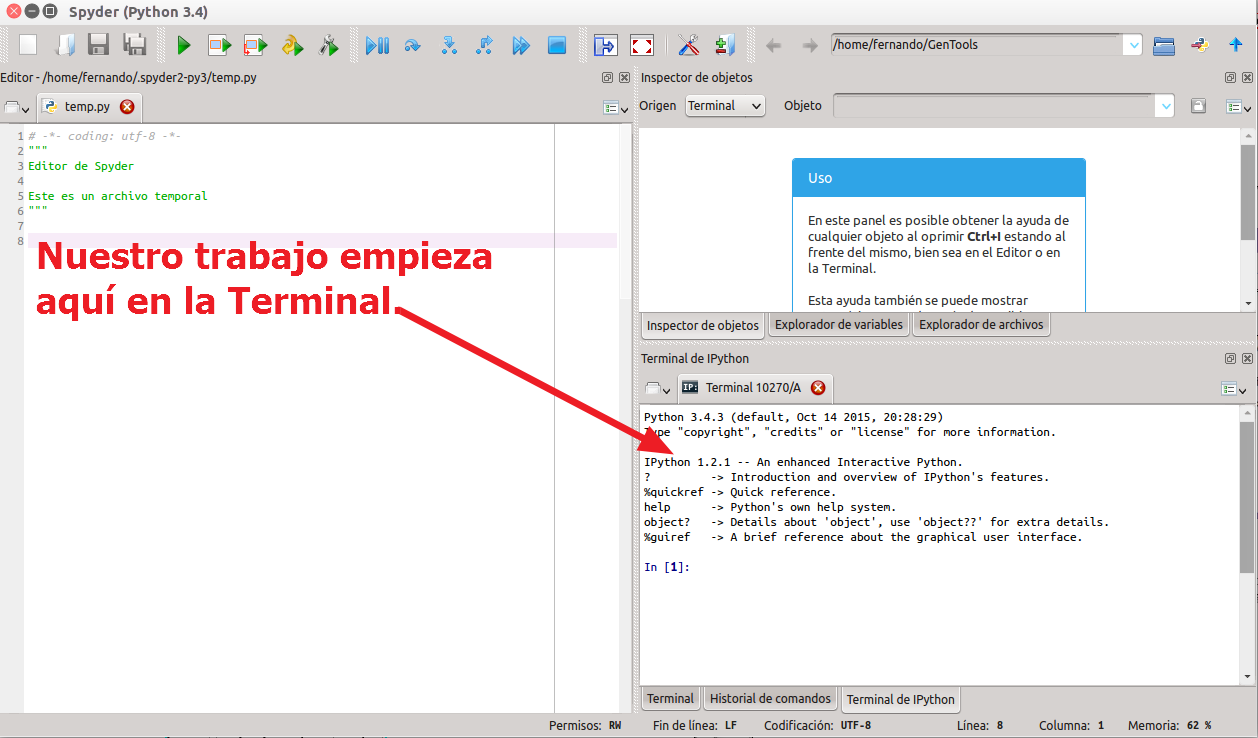
\includegraphics[width=10cm]{../fig/Tut-02-py-01-a-SpyderLinux.png}
\end{center}

La versión de Spyder que aparece en esa figura es la de Linux (Ubuntu), pero si usas otro sistema la ventana será muy parecida. Esas es una de las primeras ventajas de Spyder: una vez que un programador se acostumbra a usarlo, si tiene que cambiar de sistema operativo la adaptación resulta más fácil. 

Nuestro trabajo va a empezar, como hemos indicado en la figura, en el panel de Spyder llamado {\em Terminal}. Las primeras líneas muestran información sobre la versión de Python que estamos usando, y sugieren algunas formas de obtener ayuda. Más adelante volveremos sobre algunas de ellas. Por el momento, la línea que más nos interesa es la última, en la que aparece:
\begin{knitrout}
\definecolor{shadecolor}{rgb}{0.969, 0.969, 0.969}\color{fgcolor}\begin{kframe}
\begin{alltt}
In [1]:
\end{alltt}
\end{kframe}
\end{knitrout}
El símbolo {\tt In [1]:} es el {\tt prompt} de IPython. La palabra {\tt In} indica que Python está esperando que teclees un comando ({\em entrada de comandos}) y el {\tt [1]} indica que este será el primer comando de nuestra sesión de trabajo en IPython. Haz click con el ratón a la derecha de esa línea, hasta que veas el cursor parpadeando. En ese momento Python está esperando para empezar a dialogar con nosotros. Empecemos: rueba a teclear {\tt 2 + 3} y pulsar {\em Enter}. El resultado será el que se muestra en el rectángulo gris justo aquí debajo:

\begin{knitrout}
\definecolor{shadecolor}{rgb}{0.969, 0.969, 0.969}\color{fgcolor}\begin{kframe}
\begin{alltt}
In [1]: 2 + 3
Out[1]: 5

In [2]:
\end{alltt}
\end{kframe}
\end{knitrout}
Como ves, Python ha contestado inmediatamente debajo de la primera línea de entrada, añadiendo una {\em línea de salida:}
\begin{knitrout}
\definecolor{shadecolor}{rgb}{0.969, 0.969, 0.969}\color{fgcolor}\begin{kframe}
\begin{alltt}
\hlstd{Out[}\hlnum{1}\hlstd{]}\hlopt{:} \hlnum{5}
\end{alltt}
\end{kframe}
\end{knitrout}
con el resultado de la suma y el mismo número entre corchetes. Más adelante aprenderemos la utilidad de estos números. Además, y para que podamos seguir trabajando, IPython muestra la siguiente línea de entrada 
\begin{knitrout}
\definecolor{shadecolor}{rgb}{0.969, 0.969, 0.969}\color{fgcolor}\begin{kframe}
\begin{alltt}
In [2]:  
\end{alltt}
\end{kframe}
\end{knitrout}
en la que el cursor parpadea, a la espera de nuestra siguiente instrucción.

Por cierto, los espacios en blanco entre los números y el símbolo de operación {\tt +} son irrelevantes. Se obtiene lo mismo si usas {\tt 2+3} en lugar de {\tt 2 + 3}.  Una de las ventajas de  esta propiedad de los espacios es que podemos usarla para hacer más legible el código que escribimos. Más adelante veremos otros casos en  los que, por contra, los espacios son fundamentales. Pero no te preocupes, es fácil aprender a distinguir esos casos.

Aparte de sumas podemos hacer, naturalmente, multiplicaciones y divisiones. Prueba a ejecutar la instrucción del siguiente rectángulo gris. Puedes copiar y pegar directamente desde aquí a la consola de IPython:
\begin{knitrout}
\definecolor{shadecolor}{rgb}{0.969, 0.969, 0.969}\color{fgcolor}\begin{kframe}
\begin{alltt}
\hlnum{6} \hlopt{*} \hlnum{5}
\end{alltt}
\end{kframe}
\end{knitrout}
Python usa el asterisco para representar la multiplicación, así que el resultado es 30. De la misma forma, Python usa la barra {\tt /} para indicar la división. Compruébalo ejecutando:
\begin{knitrout}
\definecolor{shadecolor}{rgb}{0.969, 0.969, 0.969}\color{fgcolor}\begin{kframe}
\begin{alltt}
\hlnum{16} \hlopt{/} \hlnum{5}
\end{alltt}
\end{kframe}
\end{knitrout}
El resultado {\tt 3.2} de la división muestra la forma en la que Python escribe los decimales, con punto separando la parte entera y la parte decimal. Puesto que estamos usando la versión 3 de Python, el resultado de una divsión hecha con {\tt /} es siempre un número decimal. Prueba la siguiente operación:
\begin{knitrout}
\definecolor{shadecolor}{rgb}{0.969, 0.969, 0.969}\color{fgcolor}\begin{kframe}
\begin{alltt}
\hlnum{16} \hlopt{/} \hlnum{4}
\end{alltt}
\end{kframe}
\end{knitrout}
Si alguna vez tienes que usar la versión 2 de Python descubrirás que allí la división usando {\tt /} es un poco más complicada. Por el momento, seguiremos adelante sin preocuparnos de esto. Más adelante daremos más detalles.

Vamos a elevar un número al cubo. En muchos lenguajes de programación las potencias se indican con el símbolo \verb#^# (el acento circunflejo). Pero Python utiliza dos asteriscos: {\tt **}. Prueba a ejecutar esta operación:

\begin{knitrout}
\definecolor{shadecolor}{rgb}{0.969, 0.969, 0.969}\color{fgcolor}\begin{kframe}
\begin{alltt}
\hlnum{3}\hlopt{**}\hlnum{2}
\end{alltt}
\end{kframe}
\end{knitrout}
Por cierto y aunque esto es una manía personal, fíjate en que en todos los casos hemos usado espacios entre el operador y los números (operandos), salvo precisamente en este último caso de la potencia. La razón para trabajar así es porque creo que de esa forma el código resulta más legible.

\subsubsection*{División entera: resto y cociente.}

En alguna ocasión tendremos necesidad de calcular el cociente y el resto de una división entera. Por ejemplo, para convertir un tiempo en segundos al formato minutos-segundos. En Python 3 el cociente se obtiene con {\tt //} y el resto con \verb#%#. Así, un experimento que dura 475 segundos, expresado en el formato minutos-segundos dura:
\begin{knitrout}
\definecolor{shadecolor}{rgb}{0.969, 0.969, 0.969}\color{fgcolor}\begin{kframe}
\begin{alltt}
In [3]: 475 // 60
Out[3]: 7

In [4]: 475 % 60
Out[4]: 55
\end{alltt}
\end{kframe}
\end{knitrout}
Es decir, que el experimento dura 55 minutos y 7 segundos. 


\subsubsection*{Sobre la numeración del prompt de Python en estos tutoriales.}

Es posible que te haya sorprendido ver el prompt 
\begin{knitrout}
\definecolor{shadecolor}{rgb}{0.969, 0.969, 0.969}\color{fgcolor}\begin{kframe}
\begin{alltt}
In [3]:
\end{alltt}
\end{kframe}
\end{knitrout}
en el fragmento anterior de código. Si has ido ejecutando cada uno de los fragmentos de código que hemos visto hasta ahora tú debes estar viendo números mayores que 3. Pero el número concreto que aparece en la terminal no es importante y, desde luego, no influye en la respuesta de Python. Así que queremos aprovechar este momento para señalar, antes de seguir adelante, que no debes preocuparte si los números de línea en nuestros ejemplos no coinciden con los que aparecen en tu terminal de Python.   

\subsubsection*{Detalles adicionales sobre la terminal de Python en Spyder.}

En raras ocasiones la terminal no responde, o se queda en blanco sin que veamos el prompt, etc. En esos casos te recomiendo que abras una nueva terminal, pulsando {\tt Ctrl + T} (en Mac OS X, usa 
\includegraphics[height=0.3cm]{../fig/Tuts-SimboloComandoMac.png} {\tt + T}) o haciendo click con el botón derecho del ratón en la parte superior de la pestaña de la terminal, como ilustra esta figura, y seleccionando la ocpión correspondiente. No olvides cerrar la antigua terminal antes de seguir trabajando. 
\begin{center}
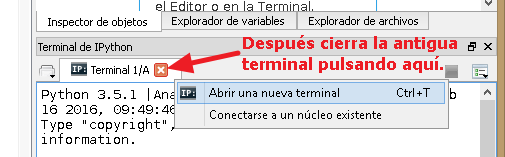
\includegraphics[height=3cm]{../fig/Tut-02-py-26-SpyderAbrirNuevaTerminal.png}
\end{center}
Otro problema que puede estar empezando a aparecer en tu trabajo es el tamaño de la terminal de Python en Spyder. Puesto que Spyder reparte el espacio de su ventana entre varios paneles, puede que el panel de terminal te resulte demasiado pequeño para ser cómodo (especialmente si trabajas en un ordenador portátil con una pantalla no demasiado grande). Y aunque puedes desplazarte arriba y abajo en el terminal con las flechas de desplazamiento del teclado (o con la rueda del ratón) hay un remedio más sencillo y cómodo. Haz clic con el ratón en este icono de la barra de herramientas de Spyder:
\begin{center}

\includegraphics[height=1cm]{../fig/Tut-02-py-19-IconoMaximizarPanel.png}
\end{center}
Al hacerlo verás que el panel de la terminal se expande hasta llenar caso toda la ventana de Spyder. 
\begin{center}
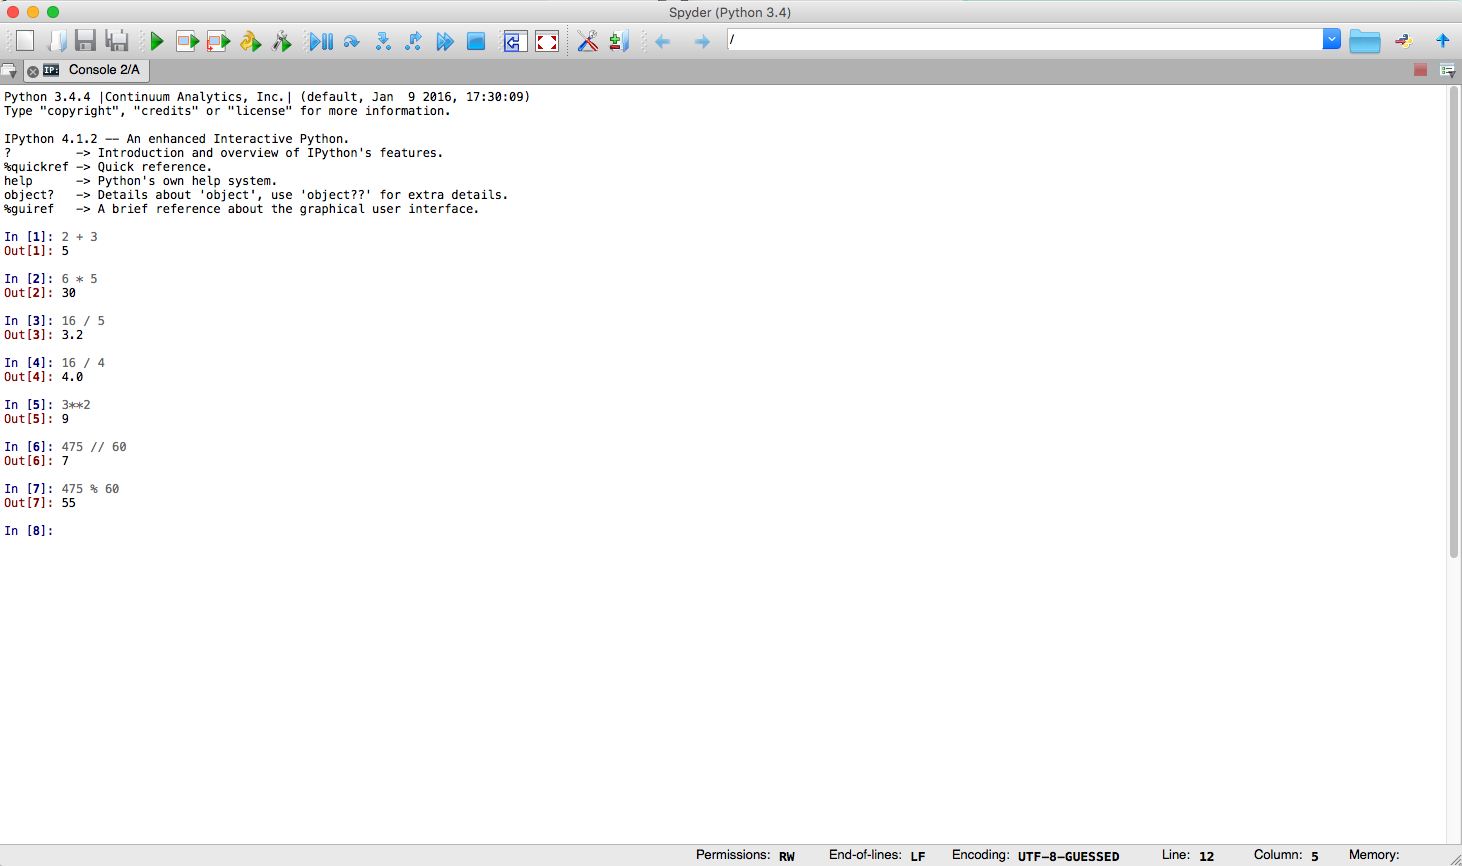
\includegraphics[width=12cm]{../fig/Tut-02-py-20-PanelTerminalMaximizado.png}
\end{center}


El proceso es reversible: otro click en el mismo icono y vuelves a la situación anterior. Y además, aunque por el momento no los estamos usando, puedes aplicar la misma idea a los otros paneles de Spyder. 




\subsection{Funciones matemáticas y módulos de Python.}
\label{tut02:subsec:FuncionesMatematicasModulosPython}

Aparte de las cuatro operaciones aritméticas básicas, las calculadoras científicas de mano incluyen funciones como la raíz cuadrada, logaritmos, funciones trigonométricas, etc. En Python, por supuesto, también podemos calcular esas funciones. Pero antes de hacerlo tenemos que aprender algo sobre el sistema de módulos de Python.

Siendo un lenguaje de programación de {\em propósito general} (es decir, no especializado en una tarea muy concreta), Python se puede utilizar para una gran cantidad de cosas distintas, cada una con sus necesidades específicas. Los programadores de Python han desarrollado muchísimas herramientas orientadas al cálculo científico, pero también a operaciones financieras, gestión de servidores web y sistemas, trabajo con bases de datos, etc. Si cada vez que usamos Python tuviéramos que instalar todo ese código estaríamos desperdiciando una enorme cantidad de recursos y haciendo que el resultado fuera poco eficiente. Al fin y al cabo el usuario que quiere utilizar Python para Genómica no necesitará, seguramente, las funciones financieras más especializadas de Python (al menos, no a la vez). Por eso, como sucede en otros lenguajes, Python está organizado en una estructura modular, de manera que en cada momento podemos disponer de aquellas partes del código de Python que necesitamos. Concretamente, el código se organiza en {\sf módulos} que puedes imaginar como cajas de herramientas. Y cuando queremos utilizar una herramienta concreta debemos indicárselo a Python pidiéndole que {\sf importe} el módulo que contiene esa herramienta.

Veamos un ejemplo. Muchas funciones matemáticas, como la raíz cuadrada y otras que mencionábamos antes, están guardadas en un módulo (caja de herramientas) llamado {\tt math}. La función raíz cuadrada se llama {\tt sqrt} (del inglés {\em square root}).  Para importar la función {\tt sqrt} del módulo {\tt math} en Python usamos este comando:
\begin{knitrout}
\definecolor{shadecolor}{rgb}{0.969, 0.969, 0.969}\color{fgcolor}\begin{kframe}
\begin{alltt}
from math import sqrt
\end{alltt}
\end{kframe}
\end{knitrout}
Cuando lo ejecutes aparentemente no pasará nada, verás algo como lo que se muestra a continuación. Recuerda que los números entre corchetes pueden ser distintos en la terminal de IPython (y que esta observación vale para todos los fragmentos de código que aparezcan a partir de ahora en los tutoriales):
\begin{knitrout}
\definecolor{shadecolor}{rgb}{0.969, 0.969, 0.969}\color{fgcolor}\begin{kframe}
\begin{alltt}
In [5]: from math import sqrt

In [6]:
\end{alltt}
\end{kframe}
\end{knitrout}
Hemos incluido la sugiente línea de entrada para que veas que debajo de {\tt In[5]} no hay un {\tt Out[5]},  no existe la correspondiente línea de salida. Pero aún así la instrucción ha hecho efecto: esa instrucción es nuestra forma de decir, en lenguaje Python, {\em ``saca la herramienta {\tt sqrt} de la caja {\tt math}''}. Una vez hecho esto, podemos usar la herramienta para, por ejemplo, calcular la ráiz cuadrada de 9 o cualquier otra. Compruébalo ejecutando esta operación:
\begin{knitrout}
\definecolor{shadecolor}{rgb}{0.969, 0.969, 0.969}\color{fgcolor}\begin{kframe}
\begin{alltt}
\hlkwd{sqrt}\hlstd{(}\hlnum{9}\hlstd{)}
\end{alltt}
\end{kframe}
\end{knitrout}
y también esta:
\begin{knitrout}
\definecolor{shadecolor}{rgb}{0.969, 0.969, 0.969}\color{fgcolor}\begin{kframe}
\begin{alltt}
\hlkwd{sqrt}\hlstd{(}\hlnum{17}\hlstd{)}
\end{alltt}
\end{kframe}
\end{knitrout}
Como ves, la función se ejecuta o {\sf invoca} colocando su argumento entre paréntesis. El módulo {\tt math} contiene muchas otras funciones además de la raíz cuadrada. Por ejemplo, las funciones trigonométricas seno, coseno y tangente que se representan, respectivamente mediante  {\tt sin}, {\tt cos} y {\tt tan}. Por defecto, esas funciones asumen que los ángulos se miden en radianes. Por su parte, el logaritmo natural (o neperiano) de base $e$ se llama en Python {\tt log} y la exponencial (para calcular $e$ elevado a un número) se llama  {\tt exp}.

Pero, además de funciones, a menudo los módulos de Python contienen otro tipo de {\em objetos}. Por ejemplo, el módulo {\tt math} contiene valores aproximados de las constantes matemáticas $\pi$ y $e$, entre otras.

Recuerda que para usar estas herramientas las debemos empezar por importarlas. Para hacer más cómodo nuestro trabajo, podemos importar varias funciones de una vez:
\begin{knitrout}
\definecolor{shadecolor}{rgb}{0.969, 0.969, 0.969}\color{fgcolor}\begin{kframe}
\begin{alltt}
from math import sin, cos, tan, log, exp, pi, e
\end{alltt}
\end{kframe}
\end{knitrout}
Una vez hecho esto podemos empezar a usar las funciones. Por ejemplo, en trigonometría elemental hemos aprendido que:
$$\sin\left(\dfrac{\pi}{4}\right) = \dfrac{\sqrt{2}}{2}\approx 0.7071$$
Vamos a calcular con Python este número de dos formas. Ejecuta primero esta versión :
\begin{knitrout}
\definecolor{shadecolor}{rgb}{0.969, 0.969, 0.969}\color{fgcolor}\begin{kframe}
\begin{alltt}
\hlkwd{sin}\hlstd{(pi}\hlopt{/}\hlnum{4}\hlstd{)}
\end{alltt}
\end{kframe}
\end{knitrout}
cuyo resultado es:
\begin{knitrout}
\definecolor{shadecolor}{rgb}{0.969, 0.969, 0.969}\color{fgcolor}\begin{kframe}
\begin{verbatim}
0.7071067811865475
\end{verbatim}
\end{kframe}
\end{knitrout}
Y después ejecuta:
\begin{knitrout}
\definecolor{shadecolor}{rgb}{0.969, 0.969, 0.969}\color{fgcolor}\begin{kframe}
\begin{alltt}
\hlkwd{sqrt}\hlstd{(}\hlnum{2}\hlstd{)}\hlopt{/}\hlnum{2}
\end{alltt}
\end{kframe}
\end{knitrout}
cuyo resultado es:
\begin{knitrout}
\definecolor{shadecolor}{rgb}{0.969, 0.969, 0.969}\color{fgcolor}\begin{kframe}
\begin{verbatim}
0.7071067811865476
\end{verbatim}
\end{kframe}
\end{knitrout}
¡Fíjate en que las últimas cifras son distintas! Eso nos debe servir de recordatorio de que los cálculos que estamos realizando son {\em aproximaciones numéricas}, no valores exactos.

Enseguida vamos a seguir avanzando hacia la Estadística. Pero antes vamos a hacer un ejercicio y, tomando como punto de partida los resultados del ejercicio, nos detendremos un poco en algunos aspectos técnicos relacionados con el módulo {\tt math} y el uso de funciones, aspectos que nos resultarán muy útiles más adelante.

\begin{ejercicio}
\label{tut02:ejercicio01}
\quad\\
En este ejercicio vamos a utilizar las líneas de  código que aparecen a continuación. Copia o teclea cada línea en el prompt (¡practica las dos maneras!), una por una, y ejecútalas, pulsando {\tt Entrar} tras copiar o teclear cada línea. Trata de adivinar el resultado de cada operación antes de ejecutar el código:
\begin{knitrout}
\definecolor{shadecolor}{rgb}{0.969, 0.969, 0.969}\color{fgcolor}\begin{kframe}
\begin{alltt}
2 + 3
15 - 7
4 * 6
13 / 5
13 // 5
13 % 5
1 / 3 + 1 / 5
\hlkwd{sqrt}(25)
\hlkwd{sqrt}(26)
\hlkwd{sin}(pi)
\hlkwd{sin}(3.14)
\end{alltt}
\end{kframe}
\end{knitrout}
\qed
%Solución en la página \pageref{tut02:ejercicio01:sol}.
\end{ejercicio}

\subsubsection*{Prioridad de los operadores.}


Fíjate en que en el ejercicio anterior Python ha interpretado el símbolo
\begin{knitrout}
\definecolor{shadecolor}{rgb}{0.969, 0.969, 0.969}\color{fgcolor}\begin{kframe}
\begin{alltt}
\hlnum{1} \hlopt{/} \hlnum{3} \hlopt{+} \hlnum{1} \hlopt{/} \hlnum{5}
\end{alltt}
\end{kframe}
\end{knitrout}
como la operación
\[\dfrac{1}{3} + \dfrac{1}{5},\]
en lugar de darle otras interpretaciones posibles como, por ejemplo:
\[\dfrac{1}{\left(\dfrac{3 + 1}{5}\right)}.\]
Para hacer esa interpretación Python ha aplicado una serie de reglas, de lo que se conoce como {\sf prioridad de operadores}, y que dicen en que orden se realizan las operaciones, según el tipo de operador. No queremos entretenernos con esto ahora, pero podemos hacer un resumen básico diciendo que en operaciones como las que hemos visto:
\begin{enumerate}
\item Primero se calculan los valores de las funciones.
\item A continuación se evalúan productos y cocientes.
\item Finalmente se evalúan sumas y restas.
\item Dentro de cada uno de los pasos anteriores, siempre se avalúan las operaciones  por orden de izquierda a derecha.
\end{enumerate}
En caso de duda, o si necesitas alterar ese orden de las operaciones, siempre puedes (y a menudo, debes) usar paréntesis para despejar la posible ambigüedad. Por ejemplo, para distinguir entre las dos interpretaciones que hemos dado, puedes escribir:
\begin{knitrout}
\definecolor{shadecolor}{rgb}{0.969, 0.969, 0.969}\color{fgcolor}\begin{kframe}
\begin{alltt}
\hlstd{(}\hlnum{1} \hlopt{/} \hlnum{3}\hlstd{)} \hlopt{+} \hlstd{(}\hlnum{1} \hlopt{/} \hlnum{5}\hlstd{)}
\end{alltt}
\end{kframe}
\end{knitrout}
o, por el contrario,
\begin{knitrout}
\definecolor{shadecolor}{rgb}{0.969, 0.969, 0.969}\color{fgcolor}\begin{kframe}
\begin{alltt}
\hlnum{1} \hlopt{/} \hlstd{((}\hlnum{3}\hlopt{+}\hlnum{1}\hlstd{)} \hlopt{/} \hlnum{5}\hlstd{)}
\end{alltt}
\end{kframe}
\end{knitrout}
Un uso prudente de paréntesis y espacios en las operaciones es una marca característica del buen hacer, cuando se escribe código en un ordenador.

\begin{ejercicio}
\label{tut02:ejercicio02}
\quad\\
Ejecuta esas dos operaciones para comprobar que obtienes los resultados esperados.
Solución en la página \pageref{tut02:ejercicio02:sol}.
\qed
\end{ejercicio}


\subsubsection*{Notación científica.}
\label{tut02:subsubsec:notacionCientifica}

El resultado del cálculo de {\tt sin(pi)} en el ejercicio anterior es {\tt 1.2246467991473532e-16}. La notación que se usa en la respuesta es la forma típica de traducir la notación científica a los lenguajes de ordenador y calculadoras. Ese símbolo representa al número:
\[
1.2246467991473532\cdot 10^{−16},
\]
de manera que el número $−16$, que sigue a la letra e en esta representación, es el exponente de 10 (también llamado {\sf orden de magnitud}), mientras que el número $1.2246467991473532$ se denomina a veces {\sf mantisa}. Puedes leer más sobre la notación científica en este artículo de la Wikipedia:
\begin{center}
      \link{http://es.wikipedia.org/wiki/Notaci\%C3\%B3n\_cient\%C3\%ADfica}{http://es.wikipedia.org/wiki/Notación\_científica}
\end{center}
En cualquier caso, el exponente {\tt -16} nos indica que se trata de un número extremadamente cercano a $0$. Recuerda que este resultado es una {\em aproximación} al valor exacto de $\sin(\pi)$, que es $0$. El propio símbolo {\tt pi} de Python representa una aproximación y no debes confundirlo con el valor exacto de $\pi$ en Matemáticas. Fíjate además en que si usas $3.14$ como aproximación de $\pi$ (como hemos hecho en el ejercicio), la respuesta, aunque pequeña, es todavía del orden de milésimas.

\subsubsection*{Errores en Python.}
\label{tut02:subsubsec:ErroresPython}

Al trabajar con Python, como con cualquier otro lenguaje de programacion, la aparición de errores es inevitable. Así que es conveniente saber lo que ocurre cuando le pedimos a Python una operación para la que no tiene respuesta. Por ejemplo, mira lo que sucede al ejecutar el siguiente código, que trata de dividir por cero:
\begin{knitrout}
\definecolor{shadecolor}{rgb}{0.969, 0.969, 0.969}\color{fgcolor}\begin{kframe}
\begin{alltt}
In [11]: 3 / 0
---------------------------------------------------------------------------
ZeroDivisionError                         \hlkwd{Traceback} (most recent call last)
<ipython-input-11-2b706ee9dd8e> in <module>()
----> 1 3 / 0

ZeroDivisionError: division by zero

In [12]:
\end{alltt}
\end{kframe}
\end{knitrout}
En este caso hemos mostrado todo el contenido de la consola desde la línea de entrada que produce el error, el consiguiente mensaje de error de Python y la siguiente línea de entrada de esa sesión. Como ves, Al hacerlo contesta con un mensaje de error que contiene una descripción más o menos detallada del tipo de error que se ha producido, en este caso {\tt ZeroDivisionError}, y del punto concreto donde ha ocurrido el error (lo cual será muy útil cuando empecemos a escribir fragmentos de código más largos).

Veamos otros ejemplos de errores en el siguiente ejercicio.
\begin{ejercicio}
\label{tut02:ejercicio03}
\quad\\
Ejecuta consecutivamente estos comandos de Python, que producirán cada uno distintos tipos de errores, y fíjate en esos errores:
\begin{knitrout}
\definecolor{shadecolor}{rgb}{0.969, 0.969, 0.969}\color{fgcolor}\begin{kframe}
\begin{alltt}
\hlkwd{log}\hlstd{(}\hlopt{-}\hlnum{1}\hlstd{)}
\end{alltt}
\end{kframe}
\end{knitrout}
\begin{knitrout}
\definecolor{shadecolor}{rgb}{0.969, 0.969, 0.969}\color{fgcolor}\begin{kframe}
\begin{alltt}
4/*3
\end{alltt}
\end{kframe}
\end{knitrout}
\begin{knitrout}
\definecolor{shadecolor}{rgb}{0.969, 0.969, 0.969}\color{fgcolor}\begin{kframe}
\begin{alltt}
\hlkwd{ln}\hlstd{(}\hlnum{7}\hlstd{)}
\end{alltt}
\end{kframe}
\end{knitrout}
%Solución en la página \pageref{tut02:ejercicio03:sol}.
\qed
\end{ejercicio}

\subsubsection*{Ayuda con Python.}
\label{tut02:subsubsec:ayudaPython}

¿Cómo se llaman las funciones de Python que calculan el arcotangente o el logaritmo en base 10? La respuesta a esta y a muchas otras preguntas está en Internet, y los buscadores son nuestros mejores aliados. Si hacemos la pregunta correcta, a menudo la primera respuesta de un buscador contendrá la información necesaria. Ten en cuenta que muchos de esos recursos están en inglés.

En cualquier caso, existen algunos recursos sobre Python que es bueno conocer. El principal de ellos es la página oficial del lenguaje, situada en:
\begin{center}
\link{https://www.python.org/}{https://www.python.org/}
\end{center}
y que contiene la documentación sobre los módulos oficiales con Python, tanto en la versión 2 como la 3. Por ejemplo, el módulo {\tt math}, para la versión 3 de Python, está documentado en:
\begin{center}
\link{https://docs.python.org/3/library/math.html}{https://docs.python.org/3/library/math.html}
\end{center}

\begin{ejercicio}
\label{tut02:ejercicio04}
\quad\\
Busca la respuesta a la pregunta que hemos dejado pendiente: ¿cómo se llaman las funciones de Python que calculan el arcotangente o el logaritmo en base 10?
%Solución en la página \pageref{tut02:ejercicio04:sol}.
\qed
\end{ejercicio}

Otro recurso interesante son los foros (en inglés) de
\begin{center}
\link{http://www.stackoverflow.com}{www.stackoverflow.com}
\end{center}
No se trata de un foro más, donde cualquiera, con más o menos conocimientos puede opinar lo primero que se le ocurra. Es una comunidad con ciertas reglas y costumbres. Pero los usuarios que responden a las preguntas de esos foros son a menudo algunos de los mayores expertos del tema en concreto y las preguntas y respuestas son visibles para todos, pertenezcan o no a la comunidad y aparecen a menudo en los primeros lugares al usar un buscador. Precisamente por eso los mencionamos: si tu pregunta ya ha sido respondida en {\em stackoverflow}, seguramente la respuesta será muy detallada; abrumadoramente detallada en ocasiones. La comunidad de usuarios no está exenta de la inclinación natural de los humanos a pavonearse. Pero en cualquier caso, suelen ser discusiones interesantes de leer. Y tal vez con el tiempo tus preguntas lleguen a ser tan buenas que merezcan una discusión a fondo en stackoverflow. Aunque la comunidad de {\em stackoverflow} se centra en la programación, existen comunidades similares para otros temas. Por ejemplo {\em Biostars} para Genómica, {\em Cross Validated} para Estadística y Análisis de Datos, etc. 

Finalmente, el propio Spyder nos puede proporcionar ayuda. Pero es mejor esperar a aprender un poco más sobre Python antes de usarla.

\subsection{Más formas de importar funciones.}
\label{tut02:subsec:MasFormasImportarFunciones}

Recuerda que hemos visto que para usar funciones del módulo {\tt math} tienes que usar una instrucción como:
\begin{knitrout}
\definecolor{shadecolor}{rgb}{0.969, 0.969, 0.969}\color{fgcolor}\begin{kframe}
\begin{alltt}
from math import sqrt, sin, cos, tan, log, exp, pi, e
\end{alltt}
\end{kframe}
\end{knitrout}

Es posible que te estés preguntando: "¿si voy a usar muchas funciones matemáticas tengo que importarlas escribiendo uno a uno el nombre de cada una de ellas?". Para evitar eso, que más adelante resultaría muy incómodo, Python proporciona varias formas alternativas de importar funciones desde un módulo.

En primer lugar, podemos decirle a Python que queremos importar {\em todas} las funciones de un módulo. Por ejemplo, para importar todas las funciones del módulo {\tt math} usaríamos:
\begin{knitrout}
\definecolor{shadecolor}{rgb}{0.969, 0.969, 0.969}\color{fgcolor}\begin{kframe}
\begin{alltt}
import math
\end{alltt}
\end{kframe}
\end{knitrout}
El módulo {\tt math} contiene una función llamada {\tt sinh}, que sirve para calcular el seno hiperbólico de un número. No te preocupes si no sabes qué es y para qué sirve, es sólo un ejemplo; si te pica la curiosidad puedes ver su definición en la Wikipedia:
\begin{center}
\link{https://es.wikipedia.org/wiki/Seno_hiperbólico}{https://es.wikipedia.org/wiki/Seno\_hiperbólico}.
\end{center}
La función seno hiperbólico cumple:
$$\sinh(0) = 0$$
Así que, dado que supuestamente  hemos importado todas las funciones del módulo {\tt math}, deberíamos poder ejecutar este código y obtener 0 como respuesta (al menos aproximadamente).
Sin embargo si ejecutas ese código verás que Python te espeta un mensaje de error inesperado:
\begin{knitrout}
\definecolor{shadecolor}{rgb}{0.969, 0.969, 0.969}\color{fgcolor}\begin{kframe}
\begin{alltt}
In [10]: import math

In [11]: \hlkwd{sinh}(0)
---------------------------------------------------------------------------
NameError                                 \hlkwd{Traceback} (most recent call last)
<ipython-input-11-f6b21eaa19a1> in <module>()
----> 1 \hlkwd{sinh}(0)

NameError: name \hlstr{'sinh'} is not defined
\end{alltt}
\end{kframe}
\end{knitrout}
Como ves, Python dice que {\tt name 'sinh' is not defined}. ¿Cómo es posible? Esto se debe a que la comodidad de importar todas las funciones del módulo {\tt math} a la vez tiene un precio. Al usar {\tt import math} Python en efecto ha importado todas las funciones, pero para saber de qué módulo proceden ha añadido el prefijo {\tt math} seguido de un punto al nombre de cada una de esas funciones. Así que la forma correcta de usar la función es:
\begin{knitrout}
\definecolor{shadecolor}{rgb}{0.969, 0.969, 0.969}\color{fgcolor}\begin{kframe}
\begin{alltt}
\hlstd{In [}\hlnum{12}\hlstd{]}\hlopt{:} \hlkwd{math.sinh}\hlstd{(}\hlnum{0}\hlstd{)}
\hlstd{Out[}\hlnum{12}\hlstd{]}\hlopt{:} \hlnum{0.0}
\end{alltt}
\end{kframe}
\end{knitrout}
que, como ves, ahora sí produce el resultado esperado.

\subsubsection*{Importar módulos sin prefijo. Posibles conflictos de nombre.}
\label{tut02:subsubsec:ImportarModulosSinPrefijo}

Ahora es posible que pienses que, puestas así las cosas, no hemos ganado mucho importando todas las funciones de {\tt math} a la vez. La supuesta comodidad queda en parte eclipsada por la necesidad de escribir ese prefijo {\tt math} delante de cada aparición de una función del módulo.

Creemos que es conveniente que comprendas el problema que se plantea para los desarrolladores de Python, y el compromiso que han tenido que adoptar para evitar errores imprevisibles: pronto vamos a aprender a escribir nuestras propias funciones. Y estos prefijos son necesarios para evitar conflictos entre funciones de distintos módulos que tienen el mismo nombre.

En cualquier caso, cuando estamos muy seguros de lo que hacemos podemos usar una forma distinta de importación:
\begin{knitrout}
\definecolor{shadecolor}{rgb}{0.969, 0.969, 0.969}\color{fgcolor}\begin{kframe}
\begin{alltt}
from math import *
\end{alltt}
\end{kframe}
\end{knitrout}
Esta forma de importar te recordará a la primera que hemos visto, pero ahora el asterisco juega el papel de {\em comodín}, de manera que lo que estamos diciéndole a Python es que importe todas las funciones del módulo {\tt math}, usando directamente los nombres de esas funciones, sin prefijos. Ahora puedes probar a ejecutar directamente:
\begin{knitrout}
\definecolor{shadecolor}{rgb}{0.969, 0.969, 0.969}\color{fgcolor}\begin{kframe}
\begin{alltt}
\hlkwd{sinh}\hlstd{(}\hlnum{0}\hlstd{)}
\end{alltt}
\end{kframe}
\end{knitrout}
y comprobarás que no hay errores.

\subsubsection*{Números complejos como ejemplo de conflicto de nombres.}
\label{tut02:subsubsec:NumerosComplejosConflictoNombres}

Los conflictos de nombre a los que hemos aludido antes no son un fenómeno raro. Para que veas un ejemplo sencillo vamos a usar otro módulo de Python llamado {\tt cmath} que contiene funciones para trabajar con números complejos. Podrías cargar todas las funciones de ese módulo como hemos hecho con las de {\tt math}:
\begin{knitrout}
\definecolor{shadecolor}{rgb}{0.969, 0.969, 0.969}\color{fgcolor}\begin{kframe}
\begin{alltt}
from cmath import *
\end{alltt}
\end{kframe}
\end{knitrout}
Y ahora, supongamos que quieres volver a calcular la misma raíz cuadrada $\sqrt{9}$ que vimos como primer ejemplo. ¿Qué sucede?:
\begin{knitrout}
\definecolor{shadecolor}{rgb}{0.969, 0.969, 0.969}\color{fgcolor}\begin{kframe}
\begin{alltt}
In [13]: from cmath import *

In [14]: \hlkwd{sqrt}(9)
Out[14]: (3+0j)
\end{alltt}
\end{kframe}
\end{knitrout}
La respuesta es un número complejo. No queremos entrar en detalles sobre los números complejos, porque no vamos a necesitarlos en el resto del curso. Estamos simplemente mostrando un ejemplo de cómo pueden aparecer los conflictos de nombres en cuanto se combinan varios módulos de Python, Si sabes algo sobre números complejos, lo único que debemos aclarar es que Python usa $j$ para representar la unidad imaginaria (es decir, $j^2 = -1$), la misma cantidad que a menudo se representa en los libros de matemáticas mediante $i$ (la notación $j$ es más frecuente en Física e Ingeniería).

¿Por qué ha ocurrido esto? Pues porque ambos módulos {\tt math} y {\tt cmath} tiene funciones llamadas {\tt sqrt} pero que son {\em distintas}: la de {\tt math} sirve para calcular la raíz cuadrada positiva de un número real positivo, mientras que la de {\tt cmath} calcula una raíz cuadrada de cualquier número complejo, pero la respuesta es {\em siempre} un número complejo, independientemente de que el número de partida sea real o no. Y puesto que hemos importado {\tt cmath} después de importar {\tt math}, la función {\tt sqrt} de {\tt cmath} ha remplazado a la función {\tt sqrt} de {\tt math}. Y lo que es peor, en casos como este Python no nos avisa de que una función ha remplazado a otra (otros lenguajes de programación, como R, al menos lanzan una advertencia en situaciones similares).


\begin{ejercicio}
\label{tut02:ejercicio05}
\quad\\
Vamos a comprobar el hecho de que el último módulo importado reemplaza a las anteriores funciones del mismo nombre. Vuelve a importar {\tt math} usando el método del asterisco y repite el cálculo de {\tt sqrt(9)}. ¿Qué sucede ahora?
%Solución en la página \pageref{tut02:ejercicio05:sol}.
\qed
\end{ejercicio}

Como ilustra este ejemplo, la opción de importar las funciones de un módulo usando el asterisco es a menudo demasiado arriesgada y puede producir errores difíciles de diagnosticar cuando el código en Python sea más complejo que los ejemplos básicos que estamos viendo. Especialmente cuando el código tiene más de un autor, que es la situación más habitual en el trabajo habitual. Por esa razón usar el asterisco para importar se considera una {\sf mala práctica} al programar en Python. ¡No lo hagas! Y por si te lo has preguntado, ocurre algo análogo si usas:
\begin{knitrout}
\definecolor{shadecolor}{rgb}{0.969, 0.969, 0.969}\color{fgcolor}\begin{kframe}
\begin{alltt}
from math import sqrt
\end{alltt}
\end{kframe}
\end{knitrout}
y después
\begin{knitrout}
\definecolor{shadecolor}{rgb}{0.969, 0.969, 0.969}\color{fgcolor}\begin{kframe}
\begin{alltt}
from cmath import sqrt
\end{alltt}
\end{kframe}
\end{knitrout}
La segunda función importada reemplaza a la anterior. Tenemos que resignarnos, por tanto, a utilizar los prefijos de los módulos. Es decir que tenemos que hacer:
\begin{knitrout}
\definecolor{shadecolor}{rgb}{0.969, 0.969, 0.969}\color{fgcolor}\begin{kframe}
\begin{alltt}
import math
\end{alltt}
\end{kframe}
\end{knitrout}
Y ahora usar la función raíz cuadrada mediante:
\begin{knitrout}
\definecolor{shadecolor}{rgb}{0.969, 0.969, 0.969}\color{fgcolor}\begin{kframe}
\begin{alltt}
\hlkwd{math.sqrt}\hlstd{(}\hlnum{9}\hlstd{)}
\end{alltt}
\end{kframe}
\end{knitrout}
Si queremos usar la raíz cuadrada de un número complejo hacemos:
\begin{knitrout}
\definecolor{shadecolor}{rgb}{0.969, 0.969, 0.969}\color{fgcolor}\begin{kframe}
\begin{alltt}
import cmath
\end{alltt}
\end{kframe}
\end{knitrout}
y ahora podemos calcular con:
\begin{knitrout}
\definecolor{shadecolor}{rgb}{0.969, 0.969, 0.969}\color{fgcolor}\begin{kframe}
\begin{alltt}
\hlkwd{cmath.sqrt}\hlstd{(}\hlnum{9}\hlstd{)}
\end{alltt}
\end{kframe}
\end{knitrout}
Esto no afecta a la otra función {\tt sqrt}, la de {\tt math}, que sigue funcionando sin problemas. Veámoslo en una secuencia de comandos de IPython:
\begin{knitrout}
\definecolor{shadecolor}{rgb}{0.969, 0.969, 0.969}\color{fgcolor}\begin{kframe}
\begin{alltt}
In [18]: import math

In [19]: \hlkwd{math.sqrt}(9)
Out[19]: 3.0

In [20]: import cmath

In [21]: \hlkwd{cmath.sqrt}(9)
Out[21]: (3+0j)

In [22]: \hlkwd{math.sqrt}(9)
Out[22]: 3.0
\end{alltt}
\end{kframe}
\end{knitrout}
Como ves, la segunda llamada a {\tt math.sqrt(9)} no se ve afectada por la función de {\tt cmath}.

Esta forma de trabajar elimina los conflictos de nombre entre módulos, pero puede resultar especialmente molesta con módulos de nombres largos. Por ejemplo, un poco más abajo aprenderemos a usar el módulo {\tt matplotlib} para dibujar algunas gráficas. Sería bastante molesto tener que escribir el prefijo {\tt matplotlib} cada vez que queremos usar una función de ese módulo. Para aliviar al menos parcialmente esa incomodidad Python nos permite usar un {\em alias}, normalmente una abreviatura, para importar un módulo. Por ejemplo, para importar {\tt matplotlib} usaríamos:
\begin{knitrout}
\definecolor{shadecolor}{rgb}{0.969, 0.969, 0.969}\color{fgcolor}\begin{kframe}
\begin{alltt}
import matplotlib as mp
\end{alltt}
\end{kframe}
\end{knitrout}
y entonces en lugar de usar {\tt matplotlib} como prefijo para las funciones de ese módulo basta con usar {\tt mp}. Aunque {\tt math} y {\tt cmath} son nombres de módulo relativamente cortos, vamos a usar alias aún más cortos para que nos sirvan de ejemplo de cómo funciona esta idea. LA secuencia anterior de comandos de IPython quedaría así:
\begin{knitrout}
\definecolor{shadecolor}{rgb}{0.969, 0.969, 0.969}\color{fgcolor}\begin{kframe}
\begin{alltt}
In [23]: import math as m

In [24]: \hlkwd{m.sqrt}(9)
Out[24]: 3.0

In [25]: import cmath as c

In [26]: \hlkwd{c.sqrt}(9)
Out[26]: (3+0j)

In [27]: \hlkwd{m.sqrt}(9)
Out[27]: 3.0
\end{alltt}
\end{kframe}
\end{knitrout}
Como ves, de esta forma el esfuerzo necesario para evitar conflictos es considerablemente menor.

\subsection{Algunos detalles adicionales sobre IPython.}
\label{tut02:subsec:AlgunosDetallesAdicionalesIPython}

Ya hemos dicho antes que Python es un lenguaje con una comunidad de usuarios muy amplia y que se usa de modos muy diversos, para tareas muy distintas. Eso se traduce en la existencia de multitud de herramientas distintas, cada una con sus pros y sus contras, adaptadas a esa gran diversidad del ecosistema Python. Y en particular, existen varias terminales posibles para trabajar con Python (en inglés se usa {\em shell} para referirse a la terminal). Nuestro contacto con la terminal hasta ahora se reduce a pensar en ella como un panel de Spyder que usamos para hablar con Python. Esa idea es en general correcta, pero queremos añadirle dos matices:
\begin{itemize}
  \item En primer lugar, hay terminales que {\em viven} fuera de Spyder. Muchos programadores prefieren usar una terminal independiente, conectada con otras herramientas que les gustan más. Cuando tengas experiencia podrás decidir lo qué quieres hacer.
  \item Sin salir de Spyder, puedes utilizar más de una consola o más de un tipo de consola (se abrirían como pestañas del panel que contiene a la terminal).
\end{itemize}
La terminal de comandos que estamos usando es un tipo especial de terminal, llamada {\sf IPython}. Este tipo de terminal añade algunas herramientas muy útiles al lenguaje Python básico. En este apartado vamos a empezar a ver algunas de ellas.

Si al llegar a este punto sentes una cierta confusión entre Python, IPython, Spyder, etc., no te preocupes. Es normal cuando te encuentras de golpe con muchos términos nuevos. Sigue adelante con las instrucciones que te proporcionamos y con la práctica todo irá quedando más claro.

\subsubsection*{Limpiando la memoria de Python.}
\label{tut02:subsubsec:limpiandoMemoriaPython}

Al llegar a a este punto hemos importado los módulos {\tt math} y {\tt cmath} de varias maneras y probablemente empieza a ser difícil seguirles el rastro. Y eso, al igual que ocurría con los conflictos de nombre, puede causarnos problemas en el resto de la sesión. A veces, al trabajar con con IPython, te encontrarás en una situación como esta en la que quieres hacer {\em tabla rasa} y pedirle a Python que olvide todos los pasos previos para poder empezar a trabajar sin preocuparte de ese tipo de conflictos. Afortunadamente, existe un mecanismo para hacer esto. Basta con ejecutar este comando especial:
\begin{knitrout}
\definecolor{shadecolor}{rgb}{0.969, 0.969, 0.969}\color{fgcolor}\begin{kframe}
\begin{alltt}
%reset
\end{alltt}
\end{kframe}
\end{knitrout}
Al hacerlo, IPython nos pedirá que confirmemos esa decisión. Al fin y al cabo, estaremos borrando (casi) todo el trabajo previo de esa sesión. {\bf Es muy importante entender esto.} Algunas sesiones de trabajo pueden contener cálculos muy valiosos, que tardan horas en ejecutarse, y en ese caso hacer un reset puede suponer perder todo ese trabajo. Asegúrate siempre de que realmente quieres hacer esto.  

Una vez hechas las advertencias pertinentes, adelante. Y no te preocupes, a pesar de esas advertencias enseguida vamos a enseñarte un remedio para posibles despistes.

\begin{ejercicio}
\label{tut02:ejercicio06}
\quad\\
\begin{enumerate}
\item Ejecuta el comando
\begin{knitrout}
\definecolor{shadecolor}{rgb}{0.969, 0.969, 0.969}\color{fgcolor}\begin{kframe}
\begin{alltt}
%reset
\end{alltt}
\end{kframe}
\end{knitrout}
\item Prueba a ejecutar alguna de las operaciones que hemos hecho antes. Por ejemplo:
\begin{knitrout}
\definecolor{shadecolor}{rgb}{0.969, 0.969, 0.969}\color{fgcolor}\begin{kframe}
\begin{alltt}
\hlkwd{m.sqrt}\hlstd{(}\hlnum{9}\hlstd{)}
\end{alltt}
\end{kframe}
\end{knitrout}
O también
\begin{knitrout}
\definecolor{shadecolor}{rgb}{0.969, 0.969, 0.969}\color{fgcolor}\begin{kframe}
\begin{alltt}
\hlkwd{math.sqrt}\hlstd{(}\hlnum{9}\hlstd{)}
\end{alltt}
\end{kframe}
\end{knitrout}
O incluso
\begin{knitrout}
\definecolor{shadecolor}{rgb}{0.969, 0.969, 0.969}\color{fgcolor}\begin{kframe}
\begin{alltt}
\hlkwd{sqrt}\hlstd{(}\hlnum{9}\hlstd{)}
\end{alltt}
\end{kframe}
\end{knitrout}
¿Qué sucede?
\end{enumerate}
%Solución en la página \pageref{tut02:ejercicio06:sol}.
\qed
\end{ejercicio}

Una observación, antes de seguir adelante. Los comandos que empiezan por \verb#%#,
como \verb#%reset#
se denominan {\sf comandos mágicos}. No son comandos de Python, sino de IPython y sólo sirven dentro de una terminal de IPython\footnote{ Y que los expertos nos perdonen esta simplificación. Ya veremos que en realidad sí se pueden usar fuera de la terminal.}. Más adelante volveremos sobre esto y entenderás mejor los matices de esa diferencia entre comandos mágicos y los comandos ordinarios de Python.

\subsubsection*{El historial de comandos y el tabulador para completar código.}
\label{tut02:subsubsec:historialComandosTabuladorCompletarCodigo}

Al ejecutar el comando mágico \verb#%reset#
hemos borrado, como decíamos, casi toda la memoria de nuestra sesión de trabajo con Python. Pero aunque Python no recuerde nada, IPython sí recuerda algo que puede ser muy útil y valioso para nosotros: nuestro {\sf historial de comandos}.  Para verlo, sitúate en el prompt de la terminal de IPython y pulsa varias veces la tecla de la flecha hacia arriba en tu teclado. Al hacerlo verás como van desfilando, una tras otra, las últimas instrucciones que has tecleado en IPython, empezando por las más recientes.
Y si pulsas la tecla de la flecha hacia abajo recorrerás esa lista en sentido inverso. En cualquier punto del recorrido puedes pararte y si lo deseas puedes hacer alguna modificación del comando que usaste anteriormente. Después puedes ejecutar el comando resultante (lo hayas modificado o no). Probemos esto:
\begin{ejercicio}
\label{tut02:ejercicio07}
\quad\\
Antes hemos usado Python para comprobar que:
$$\sin\left(\dfrac{\pi}{4}\right) = \dfrac{\sqrt{2}}{2}\approx 0.7071$$
Usa las flechas del teclado hasta localizar los comandos que usamos y modifícalos para comprobar estas otras identidades trigonométricas:
\[
\begin{array}{lll}
\sin\left(\dfrac{\pi}{3}\right) = \dfrac{\sqrt{3}}{2},&&
\cos\left(\dfrac{\pi}{3}\right) = \dfrac{1}{2},\\[3mm]
\sin\left(\dfrac{\pi}{6}\right) = \dfrac{1}{2},&&
\cos\left(\dfrac{\pi}{6}\right) = \dfrac{\sqrt{3}}{2}.
\end{array}
\]
%Solución en la página \pageref{tut02:ejercicio07:sol}.
\qed
\end{ejercicio}

Esta forma de navegar por el historial de comandos es muy cómoda cuando tienes que repetir un comando varias veces (quizá con pequeñas variaciones) o cuando se produce un error y debemos hacer correcciones. Además, Spyder nos proporciona una herramienta de seguridad adicional que complementa al historial de comandos de IPython y que nos puede sacar de más de un apuro. Si devuelves el panel de la terminal a su tamaño original (recuerda, con el icono 
\includegraphics[height=0.25cm]{../fig/Tut-02-py-19-IconoMaximizarPanel.png} de la barra superior de Spyder) verás que debajo de ese panel aparece una pestaña denominada 
{\sf History Log}. Haz click con el ratón sobre ella y verás que un nuevo panel ocupa el espacio de la terminal (a la qu epeudes volver con la pestaña denominada {\sf IPython console}). El panel  History Log muestra nuestro {\em historial de comandos} de esta y otras sesiones previas (las fechas y horas de comienzo de cada sesión aparecen como comentarios). La siguiente figura muestra el panel History Log de Spyder (la versión para Mac en este caso) en el que puedes ver algunos de los últimos comandos que han ejecutado en esa sesión (terminando con un \verb&%reset&).

\begin{center}
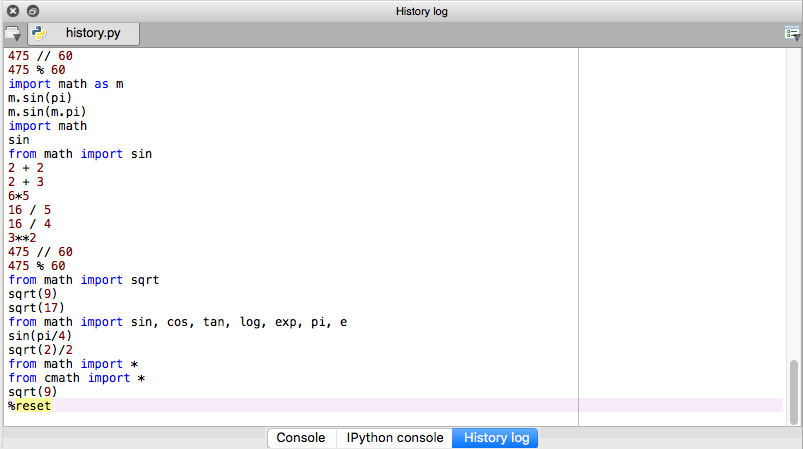
\includegraphics[width=14cm]{../fig/Tut-02-py-21-PanelHistoryLog.png}
\end{center}

Una posibilidad, si quieres poner a salvo tu trabajo, es copiar el contenido de esta ventana (al menos la parte que te interesa proteger) y pegarlo en un documento del editor de texto ({\em Bloc de Notas} o similar). Puedes guardar ese documento como copia de respaldo de tu trabajo. Pero pronto, antes del final de este tutorial, te mostraremos una manera mejor de hacer esto. Así que lo mejor es que pienses en el {\em History Log} como un último recurso a utilizar para situaciones imprevistas. Aparte de eso yo lo uso para hacer copia/pega de comandos, combinándolo con el historial de comandos.

\subsubsection*{Limpieza visual de la consola de IPython.}
\label{tut02:subsubsec:limpiezaVisualConsolaIPython}

Regresemos a la terminal. Hay otro comando mágico que tal vez quieras usar a veces al trabajar con IPython. Se trata del comando \verb#%clear#.
Su efecto se entiende mejor comparando las siguientes dos imágenes. En la de la izquierda estamos en medio de una sesión de trabajo con IPython, en la que hemos introducido diversos comandos, hemos cometido errores, etc. Y estamos justo a punto de ejecutar  \verb#%clear#.
A la derecha se muestra el resultado después de ejecutarlo:
\begin{center}
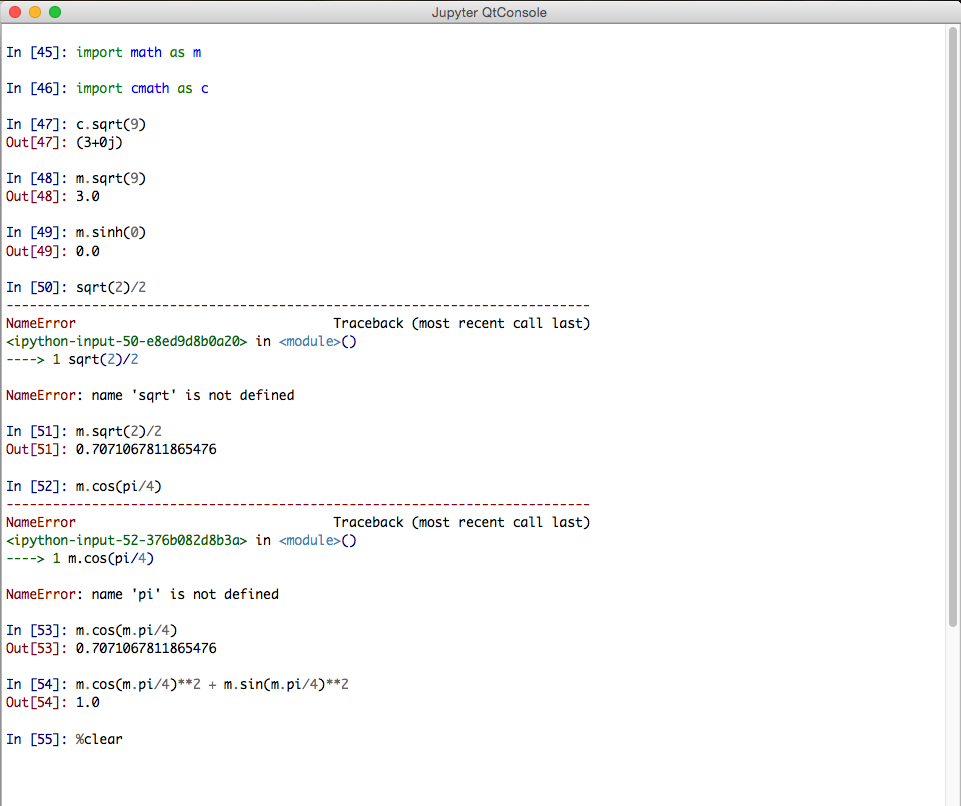
\includegraphics[width=7.3cm]{../fig/Tut-02-py-02a.png}\quad
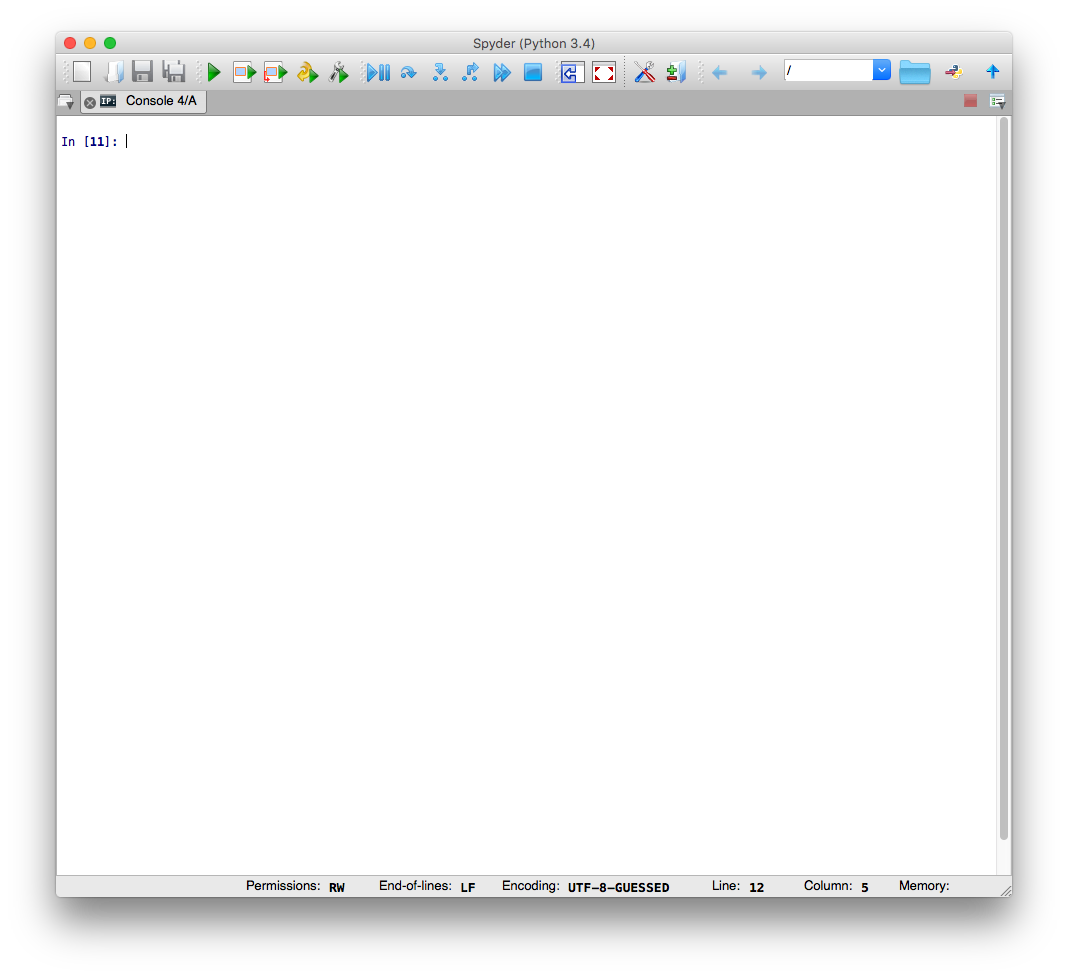
\includegraphics[width=7.3cm]{../fig/Tut-02-py-02b.png}
\end{center}
Como ves,  \verb#%clear#
limpia el contenido del panel con la terminal de IPython. A diferencia de  \verb#%reset#,
la memoria de Python no se ve afectada. Y tampoco se elimina el historial de comandos, el efecto es puramente visual. Pero a menudo nos resulta cómodo {\em ``despejar``} la pantalla para poder trabajar con más claridad.

\section{Variables y listas en Python.}
\label{tut02:sec:variablesListasPython}

En la sección previa hemos usado Python como una calculadora. Pero, para ir más allá, tenemos que disponer de {\sf estructuras de datos}. Ese término describe, en Computación, las herramientas que nos permiten almacenar y procesar información. Las estructuras de datos más básicas de Python son las {\sf variables} y las {\sf listas}. En este y en próximos tutoriales nos iremos encontrando con otras estructuras de datos: conjuntos, diccionarios, tuplas, matrices, dataframes, entre otras.

\subsection{Variables en Python.}
\label{tut02:subsec:variablesPython}

Te recomendamos que antes de seguir adelante hagas una limpieza completa en la terminal de IPython. Puedes usar los comandos mágicos \verb#%reset# y \verb#%clear#  
o, si lo prefieres, puedes simplemente cerrar Spyder y volver a abrirlo (en Anaconda no hace falta que cierres el Launcher, basta con Spyder).

Una {\sf variable} en Python es un símbolo o nombre que usamos para referirnos a un objeto. Por ejemplo, ejecuta este código:
\begin{knitrout}
\definecolor{shadecolor}{rgb}{0.969, 0.969, 0.969}\color{fgcolor}\begin{kframe}
\begin{alltt}
\hlstd{a} \hlkwb{=} \hlnum{2}
\end{alltt}
\end{kframe}
\end{knitrout}
Aparentemente no ha sucedido nada. En la consola de IPython no hay respuesta: no aparece inmediatamente una línea de salida (que empezaría por {\tt Out}). Pero a partir de ese momento Python ha {\sf asignado} el valor 2 al símbolo {\tt a}. Así que si, por ejemplo, ejecutas
\begin{knitrout}
\definecolor{shadecolor}{rgb}{0.969, 0.969, 0.969}\color{fgcolor}\begin{kframe}
\begin{alltt}
\hlstd{a} \hlopt{+} \hlnum{1}
\end{alltt}
\end{kframe}
\end{knitrout}
ahora sí que verás una línea de salida con el resultado que imaginas. La secuencia completa es esta:
\begin{knitrout}
\definecolor{shadecolor}{rgb}{0.969, 0.969, 0.969}\color{fgcolor}\begin{kframe}
\begin{alltt}
\hlstd{In [}\hlnum{1}\hlstd{]}\hlopt{:} \hlstd{a} \hlkwb{=} \hlnum{2}

\hlstd{In [}\hlnum{2}\hlstd{]}\hlopt{:} \hlstd{a} \hlopt{+} \hlnum{1}
\hlstd{Out[}\hlnum{2}\hlstd{]}\hlopt{:} \hlnum{3}
\end{alltt}
\end{kframe}
\end{knitrout}
Podemos crear una variable con una instrucción muy sencilla, como {\tt a = 2}, pero también como resultado de efectuar en el lado derecho una operación mucho más complicada. Por ejemplo, después de importar el módulo {\tt math} con el alias {\tt m} vamos a usar una variable {\tt V} para calcular el volumen de una esfera de radio $r=10cm$. Recuerda que el volumen viene dado por:
\[V = \dfrac{4}{3}\pi r^3.\]
Así que usamos estos comandos:
\begin{knitrout}
\definecolor{shadecolor}{rgb}{0.969, 0.969, 0.969}\color{fgcolor}\begin{kframe}
\begin{alltt}
In [4]: import math as m

In [5]: V = (4 / 3) * m.pi * 10**3
\end{alltt}
\end{kframe}
\end{knitrout}
Eso está muy bien, pero ¿cuánto vale {\tt V}? Hay dos formas de ver ese valor. En IPython lo más rápido es escribir el nombre de la variable y ejecutarlo como una instrucción:
\begin{knitrout}
\definecolor{shadecolor}{rgb}{0.969, 0.969, 0.969}\color{fgcolor}\begin{kframe}
\begin{alltt}
\hlstd{In [}\hlnum{6}\hlstd{]}\hlopt{:} \hlstd{V}
\hlstd{Out[}\hlnum{6}\hlstd{]}\hlopt{:} \hlnum{4188.790204786391}
\end{alltt}
\end{kframe}
\end{knitrout}
Pero también podemos usar la función {\tt print} así:
\begin{knitrout}
\definecolor{shadecolor}{rgb}{0.969, 0.969, 0.969}\color{fgcolor}\begin{kframe}
\begin{alltt}
\hlstd{In [}\hlnum{7}\hlstd{]}\hlopt{:} \hlkwd{print}\hlstd{(V)}
\hlnum{4188.790204786391}
\end{alltt}
\end{kframe}
\end{knitrout}
En este caso no hay diferencia y eso puede llevarte a pensar que el primer método nos ahorra trabajo. Y en efecto así es, siempre que busquemos una respuesta rápida, en casos sencillos y mientras estamos trabajando en IPython. Pero a medida que avancemos por los tutoriales pronto tendras ocasión de aprender más sobre {\tt print} y verás que en muchos casos es una opción mejor y en otros, sencillamente, es la única forma de llegar a la información que queremos. Un comentario más, antes de que se nos olvide: no hemos necesitado importar {\tt print} desde ningún  módulo porque es una de las funciones básicas de Python, que están disponibles {\em siempre} en cualquier sesión de trabajo.

\paragraph{Advertencia sobre Python 2:} ya dijimos en el Tutorial-00 que avisaríamos al lector cuando nos encontráramos con diferencas importantes entre Python 2 y Python 3. Pues bien, el funcionamiento de la función {\tt print} en Python 2 es distinto del que estamos mostrando aquí. Por ejemplo, en Python 2 la función no usa paréntesis. Así que es correcto escribir:
\begin{knitrout}
\definecolor{shadecolor}{rgb}{0.969, 0.969, 0.969}\color{fgcolor}\begin{kframe}
\begin{alltt}
print 2 + 3
\end{alltt}
\end{kframe}
\end{knitrout}
mientras que en Python 3 esto produciría un mensaje de error. Si vas a usar Python 2 es {\bf imprescindible} que aprendas bien esas diferencias en el uso de {\tt print}. Aquí no vamos a profundizar más allá de esta advertencia, porque como ya hemos advertido sólo vamos a usar Python 3. 

\subsubsection*{Asignaciones.}
\label{tut02:subsubsec:asignaciones}

Las instrucciones de Python como
\begin{knitrout}
\definecolor{shadecolor}{rgb}{0.969, 0.969, 0.969}\color{fgcolor}\begin{kframe}
\begin{alltt}
\hlstd{a} \hlkwb{=} \hlnum{2}
\end{alltt}
\end{kframe}
\end{knitrout}
o como
\begin{knitrout}
\definecolor{shadecolor}{rgb}{0.969, 0.969, 0.969}\color{fgcolor}\begin{kframe}
\begin{alltt}
\hlstd{V} \hlkwb{=} \hlstd{(}\hlnum{4} \hlopt{/} \hlnum{3}\hlstd{)} \hlopt{*} \hlstd{m.pi} \hlopt{*} \hlnum{10}\hlopt{**}\hlnum{3}
\end{alltt}
\end{kframe}
\end{knitrout}
que tienen la estructura:
\begin{knitrout}
\definecolor{shadecolor}{rgb}{0.969, 0.969, 0.969}\color{fgcolor}\begin{kframe}
\begin{alltt}
\hlstd{variable} \hlkwb{=} \hlstd{expresion}
\end{alltt}
\end{kframe}
\end{knitrout}
se llaman {\sf asignaciones} y decimos que se asigna el resultado de la expresión de la derecha a la variable que aparece a la izquierda. Lo más importante que hay que recordar sobre las asignaciones es que el valor que se asigna reemplaza a cualquier valor que hubiera almacenado en la variable previamente. Así, por ejemplo, si hacemos
\begin{knitrout}
\definecolor{shadecolor}{rgb}{0.969, 0.969, 0.969}\color{fgcolor}\begin{kframe}
\begin{alltt}
\hlstd{a} \hlkwb{=} \hlnum{2}
\end{alltt}
\end{kframe}
\end{knitrout}
y después
\begin{knitrout}
\definecolor{shadecolor}{rgb}{0.969, 0.969, 0.969}\color{fgcolor}\begin{kframe}
\begin{alltt}
\hlstd{a} \hlkwb{=} \hlnum{3}
\end{alltt}
\end{kframe}
\end{knitrout}
el valor {\tt 2} que inicialmente estaba asignado a la variable {\tt a} se pierde. Si no se tiene en cuenta esto es fácil cometer errores al sobrescribir valores.

\begin{ejercicio}
\label{tut02:ejercicio08}
\quad\\
¿Cuánto valen las variables {\tt a}, {\tt b} y {\tt c} al ejecutar estos comandos uno tras otro? Haz una tabla con tres columnas tituladas {\tt a}, {\tt b} y {\tt c} y anota el valor de las variables en cada paso.
\begin{knitrout}
\definecolor{shadecolor}{rgb}{0.969, 0.969, 0.969}\color{fgcolor}\begin{kframe}
\begin{alltt}
\hlstd{a} \hlkwb{=} \hlnum{2}
\hlstd{b} \hlkwb{=} \hlnum{3}
\hlstd{c} \hlkwb{=} \hlstd{a} \hlopt{+} \hlstd{b}
\hlstd{a} \hlkwb{=} \hlstd{b} \hlopt{*} \hlstd{c}
\hlstd{b} \hlkwb{=} \hlstd{(c} \hlopt{-} \hlstd{a)}\hlopt{^}\hlnum{2}
\hlstd{c} \hlkwb{=} \hlstd{a} \hlopt{*} \hlstd{b}
\end{alltt}
\end{kframe}
\end{knitrout}
Como has podido ver, al ejecutar esas asignaciones Python no produce ningún valor como resultado. ¿Se te ocurre alguna forma de comprobar los resultados que has escrito en la tabla?
%Solución en la página \pageref{tut02:ejercicio08:sol}.
\qed
\end{ejercicio}

\subsubsection*{Copiando bloques de código a IPython.}
\label{tut02:subsubsec:copiandoBloquesCodigoIPython}

Hasta ahora se supone que para trabjar en la consola de IPython has ido o copiando y pegando uno a uno o tecleando los comandos de Python que te sugeríamos. Pero cuando aparezcan fragmentos de código más largos en estos tutoriales en algún momento esa operación de copiar y pegar una a una las líneas de código resultará molesta. Hay una forma más rápida de trabajar que te permite copiar bloques enteros de código. Para practicarlo, selecciona estas cuatro líneas de código (asegúrate de que las tienes seleccionadas todas)
\begin{knitrout}
\definecolor{shadecolor}{rgb}{0.969, 0.969, 0.969}\color{fgcolor}\begin{kframe}
\begin{alltt}
\hlstd{a} \hlkwb{=} \hlnum{2}
\hlstd{b} \hlkwb{=} \hlnum{3}
\hlstd{c} \hlkwb{=} \hlstd{a} \hlopt{+} \hlstd{b}
\hlkwd{print}\hlstd{(a, b, c)}
\end{alltt}
\end{kframe}
\end{knitrout}
cópialas y pégalas en la consola de IPython. Deberías ver algo como esto:
\begin{knitrout}
\definecolor{shadecolor}{rgb}{0.969, 0.969, 0.969}\color{fgcolor}\begin{kframe}
\begin{alltt}
\hlstd{In [}\hlnum{1}\hlstd{]}\hlopt{:} \hlstd{a} \hlkwb{=} \hlnum{2}
   \hlstd{...}\hlopt{:} \hlstd{b} \hlkwb{=} \hlnum{3}
   \hlstd{...}\hlopt{:} \hlstd{c} \hlkwb{=} \hlstd{a} \hlopt{+} \hlstd{b}
   \hlstd{...}\hlopt{:} \hlkwd{print}\hlstd{(a, b, c)}
\end{alltt}
\end{kframe}
\end{knitrout}
con el cursor parpadeando tras el último paréntesis de la cuarta fila. {\bf ¡Esto es importante para lo que sigue!} Si el cursor no está situado en esa posición asegúrate de usar las flechas del teclado para llevarlo hasta ahí. 

Si el pegado no ha ido bien y el texto que has obtenido no es lo que esperabas es mejor que esperes un poco más, hasta que aprendamos a usar el editor de código de Spyder. ¡La culpa, en estos casos, no es de Spyder! Depende, entre otras cosas, del programa que uses para leer el pdf de este tutorial. En esta figura puedes ver un ejemplo de un pegado que ha ido mal, porque los saltos de líneas no se han conservado al pegar:
\begin{center}
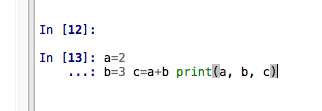
\includegraphics[width=6cm]{../fig/Tut-02-py-22-BloqueCodigoMalPegado.png}
\end{center}
Puedes desplazarte dentro de ese bloque de texto con las flechas de cursor y pulsar Enter en las posiciones en las que quieres que aparezcan saltos de línea. Pero cuando nos vemos obligados a hacer esto, arreglando {\em a mano} el código, las ventajas del copia/pega por bloques empiezan a difuminarse. 

En cualquier caso, una vez que hayas conseguido que el bloque de código aparezca correctamente y suponiendo que el cursor está situado en la última posición de la última línea de ese bloque, pulsa {\em Enter}. Aparecerá una línea en blanco más porque IPython te está dando la oportunidad de añadir más instrucciones.
\begin{knitrout}
\definecolor{shadecolor}{rgb}{0.969, 0.969, 0.969}\color{fgcolor}\begin{kframe}
\begin{alltt}
In [1]: a = 2
   ...: b = 3
   ...: c = a + b
   ...: \hlkwd{print}(a, b, c)
   ...:
\end{alltt}
\end{kframe}
\end{knitrout}
Pero como no es el caso y  no queremos añadir nada, pulsamos {\em Enter} una vez más y, ahora sí, IPython le envía a Python ese bloque de instrucciones una tras otra, Python las ejecuta y el resultado en pantalla es:
\begin{knitrout}
\definecolor{shadecolor}{rgb}{0.969, 0.969, 0.969}\color{fgcolor}\begin{kframe}
\begin{alltt}
In [1]: a = 2
   ...: b = 3
   ...: c = a + b
   ...: \hlkwd{print}(a, b, c)
   ...:
2 3 5

In [2]:
\end{alltt}
\end{kframe}
\end{knitrout}
Además de aprender a trabajar con bloques de código, hemos aprovechado este fragmento de código para ilustrar otra forma de usar la función {\tt print} para mostrar a la vez los valores de varias variables. Es posible que a la vista de esto quieras volver sobre el ejercicio \ref{tut02:ejercicio08} (pág. \pageref{tut02:ejercicio08}).

\subsubsection*{Nombres de las variables y palabras reservadas.}
\label{tut02:subsubsec:nombresVariablesPalabrasReservadas}
Aunque hasta ahora hemos usado letras como nombres de las variables, puedes utilizar nombres más descriptivos. Y muchas veces es una buena idea hacerlo. Por ejemplo,  puede que hace una semana hayas escrito estas instrucciones para resolver un problema:
\begin{verbatim}
a = 2
b = 3
c = a / b
\end{verbatim}
Pero si las vuelves a ver, pasada una semana, es muy probable que no recuerdes qué era lo que estabas tratando de conseguir al hacer esto. En cambio, al ver estas instrucciones:
\begin{verbatim}
espacio = 2
tiempo = 3
velocidad = espacio / tiempo
\end{verbatim}
es mucho más fácil reconocer el objetivo que persiguen. A lo largo de los tutoriales del curso vamos a insistir muchas veces en la necesidad de que el código esté bien {\em organizado}, y esté bien {\em documentado}. Un primer paso en esa dirección es tratar de elegir nombres descriptivos para las variables. En Python las reglas para los nombres de variables son muy flexibles: esencialmente, que empiecen por una letra y no contengan espacios ni caracteres especiales, como {\tt ?}, {\tt +}, paréntesis, etcétera. Tampoco puedes usar la ñ ni letras acentuadas\footnote{En general, también se desaconseja usar cualquiera de esos caracteres en los nombres de ficheros, carpetas, etc. Para algunos sistemas operativos no supone ningún problema, pero en otros casos puede crearte auténticos quebraderos de cabeza. Es el precio que pagamos por usar una tecnología pensada para el juego de caracteres del idioma inglés.}. Pero puedes usar un guión bajo \verb#_# como parte del nombre y a veces se hace para hacer más legibles las variables. Por ejemplo:
\begin{knitrout}
\definecolor{shadecolor}{rgb}{0.969, 0.969, 0.969}\color{fgcolor}\begin{kframe}
\begin{alltt}
\hlstd{temp_final}
\end{alltt}
\end{kframe}
\end{knitrout}
para representar la temperatura final de un proceso. Pero cuidado con los excesos. Es cierto que puedes usar nombres de variables arbitrariamente largos.  Pero si usas como nombre:
\begin{knitrout}
\definecolor{shadecolor}{rgb}{0.969, 0.969, 0.969}\color{fgcolor}\begin{kframe}
\begin{alltt}
\hlstd{Estavariablealmacenaelresultadodelaoperaciontaninteresantequeacabamosdehacer}
\end{alltt}
\end{kframe}
\end{knitrout}
tu trabajo resultará ilegible. Como siempre, se necesita un equilibrio, y con la práctica encontrarás el tuyo (consejo zen gratuito del tutorial de hoy). Para empezar, es una buena idea combinar mayúsculas y minúsculas en los nombres de las variables. Volviendo al ejemplo de la temperatura final de un proceso, el nombre {\tt temperaturafinalproceso} es menos legible y más largo que {\tt tempFinal}. Es mucho más fácil, por otra parte, que te equivoques tecleando el primero de esos nombres.

Otro aspecto que debes tener en cuenta al elegir nombres para tus variables es que no debes usar como  nombres aquellos símbolos que forman parte del propio lenguaje Python. Por ejemplo, hemos visto que en Python las palabras {\tt sqrt, import, math, from, print} se usan como parte de las instrucciones del lenguaje. Es habitual referirse a estas palabras como {\sf palabras reservadas} del lenguaje. En algunos lenguajes de programación esas palabras están de hecho reservadas y si tratas de usarlas como nombre de variable se producirá un error. Pero Python es más tolerante y te permite usar algunas de esas palabras como nombre de variable. Esa flexibilidad puede ser conveniente para programadores muy expertos, pero tú {\bf ¡no lo hagas!} No suele ser una buena idea y produce errores que pueden ser muy difíciles de detectar.  Al programar en español es fácil buscar nombres alternativos para las variables y según cuál sea tu campo de trabajo es posible que te cueste imaginar una situación en la que usarías {\tt import} como nombre de variable. Pero insistimos, procura tener cuidado con la elección de los nombres de variable para hacerlos útiles y evitar conflictos.

\subsection*{Variables de tipo cadena de caracteres.}
\label{tut02:subsection:variablesCadenaCaracteres}

En el Capítulo \ref{curso-cap:IntroduccionEstadisticaDescriptiva} del libro hemos hablado de variables cualitativas y cuantitativas. Estas últimas toman siempre valores numéricos, y las variables de Python sirven, desde luego, para almacenar esa clase de valores. Pero, como iremos viendo en sucesivos tutoriales, también se pueden utilizar variables de Python para guardar valores de variables cualitativas (factores), y otros tipos de objetos que iremos conociendo a lo largo del curso. De momento, para que veas a que nos referimos, recordaremos el Ejemplo \ref{curso-cap01:ejem:VariableCualitativaOrdenada} del libro (pág. \pageref{curso-cap01:ejem:VariableCualitativaOrdenada}), en el que teníamos una variable cualitativa ordenada que representa el pronóstico de un paciente que ingresa en un hospital. Prueba a ejecutar este código:
\begin{knitrout}
\definecolor{shadecolor}{rgb}{0.969, 0.969, 0.969}\color{fgcolor}\begin{kframe}
\begin{alltt}
\hlstd{pronostico} \hlkwb{=} \hlstr{"leve"}
\end{alltt}
\end{kframe}
\end{knitrout}
simplemente para que, de momento, veas que:
\begin{itemize}
  \item Python no protesta. El valor \verb#"leve"# es un valor perfectamente aceptable.
  \item En Python los valores que representan palabras o frases se denominan {\sf cadenas alfanuméricas}o {\sf cadenas de caracteres} (en inglés {\em character strings}, a menudo abreviado simplemente a {\em strings}). Las cadenas de caracteres se escriben siempre entre comillas. Puedes usar comillas dobles, como en \verb#"leve"# o simples, como en  \verb#'leve'#.
\end{itemize}
En los próximos tutoriales tendremos ocasión de extendernos sobre la relación entre los factores y los valores alfanuméricos de Python. Pero la utilidad de las variables de tipo alfanumérico va mucho más allá. Las usaremos pronto para añadir títulos y otras etiquetas a los gráficos o tablas, para añadir mensajes informativos a los cálculos que hagamos, etc. Y en un sentido más amplio, el procesamiento de cadenas alfanuméricas es el punto de partida de campos de trabajo como la Genómica (el genoma se representa mediante cadenas de caracteres que contienen la secuencia de bases del ADN presente en los cromosomas) o el procesamiento del lenguaje natural (el que hablamos las personas), sin el cual no dispondríamos de herramientas como buscadores avanzados de Internet, o el reconocimiento de voz, etc. Hay, por lo tanto, un mundo por descubrir cuando se trabaja con este tipo de variables, a las que apenas nos hemos asomado. Al final de este curso no serás ni mucho menos un experto, pero habrás aprendido los rudimentos del trabajo con ese tipo de variables que te permitirán pasar a textos más avanzados si lo deseas. De momento, un aperitivo.

\begin{ejercicio}
\label{tut02:ejercicio09}
\quad\\
Ejecuta estas instrucciones (recuerda que puedes copiarlas como un bloque):
\begin{knitrout}
\definecolor{shadecolor}{rgb}{0.969, 0.969, 0.969}\color{fgcolor}\begin{kframe}
\begin{alltt}
\hlstd{mensaje1} \hlkwb{=} \hlstr{"¡Hola, "}
\hlstd{usuario} \hlkwb{=} \hlstr{"Alicia"}
\hlstd{mensaje2} \hlkwb{=} \hlstr{"!, ¿cómo estás?"}
\hlkwd{print}\hlstd{(mensaje1} \hlopt{+} \hlstd{usuario} \hlopt{+} \hlstd{mensaje2)}
\end{alltt}
\end{kframe}
\end{knitrout}
¿Qué se obtiene como salida? Como puedes comprobar, la operación suma {\tt +} en el caso de cadenas de caracteres da como resultado la concatenación de esas cadenas. Prueba a cambiar la segunda línea por
\begin{knitrout}
\definecolor{shadecolor}{rgb}{0.969, 0.969, 0.969}\color{fgcolor}\begin{kframe}
\begin{alltt}
\hlstd{usuario} \hlkwb{=} \hlstr{"Luis"}
\end{alltt}
\end{kframe}
\end{knitrout}
y ejecuta de nuevo el código. Las operaciones como las de este ejemplo son frecuentes en los sistemas que producen mensajes {\em personalizados} para el usuario y, más en general, son una herramienta básica para crear textos mediante programas.


%Solución en la página \pageref{tut02:ejercicio09:sol}.
\qed
\end{ejercicio}


\subsubsection*{Tipos de variables.}
\label{tut02:subsubsection:tiposDeVariables}

En la Sección \ref{curso-cap01:subsec:VariablesCualitativasCuantitativas} del libro (pág.. \pageref{curso-cap01:subsec:VariablesCualitativasCuantitativas}) hemos discutido las diferencias entre los tipos de variables más comunes en Estadística: variables cuantitativas, que pueden ser discretas o continuas, y variables cualitativas, también llamadas factores. Python también clasifica a sus variables en tipos. Y aunque la correspondencia entre los tipos de variables en Estadística y en Python no se puede establecer automáticamente, es necesario conocer los tipos de Python para poder elegir el tipo más adecuado para representar en el código los valores de una variable estadística.

En Python las variables de tipo {\tt int} (del inglés {\em integer}, entero) sirven para almacenar números enteros (por tanto positivos, 0 o negativos). Cuando hacemos una asignación como:
\begin{knitrout}
\definecolor{shadecolor}{rgb}{0.969, 0.969, 0.969}\color{fgcolor}\begin{kframe}
\begin{alltt}
\hlstd{a} \hlkwb{=} \hlnum{12}
\end{alltt}
\end{kframe}
\end{knitrout}
Python examina el valor que estamos usando y automáticamente asigna el tipo {\tt int} a la variable {\tt a}. Para comprobar el tipo de una variable disponemos de la función {\tt type}, como puedes ver:
\begin{knitrout}
\definecolor{shadecolor}{rgb}{0.969, 0.969, 0.969}\color{fgcolor}\begin{kframe}
\begin{alltt}
\hlstd{In [}\hlnum{1}\hlstd{]}\hlopt{:} \hlstd{a} \hlkwb{=} \hlnum{12}

\hlstd{In [}\hlnum{2}\hlstd{]}\hlopt{:} \hlkwd{type}\hlstd{(a)}
\hlstd{Out[}\hlnum{3}\hlstd{]}\hlopt{:} \hlstd{int}
\end{alltt}
\end{kframe}
\end{knitrout}
¿Qué sucede cuando la variable representa un número decimal? Compruébalo:

\begin{ejercicio}
\label{tut02:ejercicio10}
Asigna el valor {\tt 7.32} a la variable {\tt b} y usa la función {\tt type} para descubrir de que tipo es la variable resultante.
%Solución en la página \pageref{tut02:ejercicio10:sol}.
\qed
\end{ejercicio}
Como has podido comprobar en este ejercicio, Python usa el tipo {\tt float} para la representación decimal de los números. Ese tipo de variables y los valores que almacenan se suelen llamar en español de {\sf coma flotante} (en inglés es {\em floating point}, de ahí el nombre {\tt float}). Los valores en notación científica que hemos visto en la página \pageref{tut02:subsubsec:notacionCientifica} también son de tipo {\tt float}.

Las variables cuantitativas discretas se representan en Python de manera natural mediante variables de tipo {\tt int}, mientras que las variables cuantitativas continuas se pueden representar con variables de tipo {\tt float}, siempre teniendo en cuenta que se trata de aproximaciones a los números reales. Una variable de tipo {\tt float} sólo puede almacenar unas cuantas cifras decimales de un número como  $\frac{1}{3}$, que en realidad tiene una representación decimal periódica $0.33333\ldots$ (con infinitas cifras). Es importante recordar esto para evitar confusiones al interpretar los resultados del código Python.

¿Qué ocurre con los factores, las variables cualitativas? Cuando un factor toma sólo $n$ valores (recuerda, decimos que el factor tiene $n$ niveles) podemos codificar esos niveles mediante los números del $1$ al $n$ y por tanto usar una variable de tipo {\tt int}. Aunque eso es sin duda posible, en otras ocasiones preferiremos usar variables de tipo cadena de caracteres, para poder asignar nombres más informativos a los niveles del factor. Es mucho más sencillo entender el código si vemos una asignación como:
\begin{knitrout}
\definecolor{shadecolor}{rgb}{0.969, 0.969, 0.969}\color{fgcolor}\begin{kframe}
\begin{alltt}
\hlstd{pronostico} \hlkwb{=} \hlstr{"leve"}
\end{alltt}
\end{kframe}
\end{knitrout}
que si viéramos en su lugar:
\begin{knitrout}
\definecolor{shadecolor}{rgb}{0.969, 0.969, 0.969}\color{fgcolor}\begin{kframe}
\begin{alltt}
\hlstd{pronostico} \hlkwb{=} \hlnum{2}
\end{alltt}
\end{kframe}
\end{knitrout}
¿De qué tipo es la variable creada al asignarle como valor una cadena de caracteres?
\begin{knitrout}
\definecolor{shadecolor}{rgb}{0.969, 0.969, 0.969}\color{fgcolor}\begin{kframe}
\begin{alltt}
\hlstd{In [}\hlnum{1}\hlstd{]}\hlopt{:} \hlstd{pronostico} \hlkwb{=} \hlstr{"leve"}

\hlstd{In [}\hlnum{2}\hlstd{]}\hlopt{:} \hlkwd{type}\hlstd{(pronostico)}
\hlstd{Out[}\hlnum{2}\hlstd{]}\hlopt{:} \hlstd{str}
\end{alltt}
\end{kframe}
\end{knitrout}
Como ves, se trata de variables de tipo {\tt str} (del inglés {\em string}, que a su vez es una abreviatura de {\em character string}, cadena de caracteres).

Hay mucho más que decir sobre la representación y el uso de los factores en Python. En futuros tutoriales volveremos sobre este tema y sobre los tipos de variables de Python en general.

Antes de cerrar este apartado, queremos mencionar que existen numerosas funciones de Python para convertir valores de un tipo de variable a otro tipo. Esas conversiones pueden ser muy útiles, pero no hay que perder de visa que en ocasiones la conversión lleva aparejada una pérdida de información. Algunas de esas funciones se llaman exactamente igual que el tipo de destino al que queremos convertir un valor. Por ejemplo, para convertir de tipo {\tt int} (entero) a {\tt float} (coma flotante) tenemos la función {\tt float}:
\begin{knitrout}
\definecolor{shadecolor}{rgb}{0.969, 0.969, 0.969}\color{fgcolor}\begin{kframe}
\begin{alltt}
\hlstd{In [}\hlnum{1}\hlstd{]}\hlopt{:} \hlkwd{float}\hlstd{(}\hlnum{7}\hlstd{)}
\hlstd{Out[}\hlnum{1}\hlstd{]}\hlopt{:} \hlnum{7.0}
\end{alltt}
\end{kframe}
\end{knitrout}
Fíjate en que el resultado muestra claramente que {\tt float} da como resultado la representación decimal del número (la representación en coma flotante, para ser precisos). ¿Y el camino inverso? Usamos la función {\tt int}:
\begin{knitrout}
\definecolor{shadecolor}{rgb}{0.969, 0.969, 0.969}\color{fgcolor}\begin{kframe}
\begin{alltt}
\hlstd{In [}\hlnum{1}\hlstd{]}\hlopt{:} \hlkwd{int}\hlstd{(}\hlnum{4.67}\hlstd{)}
\hlstd{Out[}\hlnum{1}\hlstd{]}\hlopt{:} \hlnum{4}
\end{alltt}
\end{kframe}
\end{knitrout}
Aquí tienes un ejemplo claro de pérdida de información. La conversión de como flotante a decimal implica eliminar las cifras decimales después del punto con la consiguiente pérdida de precisión. Mira otro ejemplo:
\begin{knitrout}
\definecolor{shadecolor}{rgb}{0.969, 0.969, 0.969}\color{fgcolor}\begin{kframe}
\begin{alltt}
\hlstd{In [}\hlnum{2}\hlstd{]}\hlopt{:} \hlkwd{int}\hlstd{(}\hlopt{-}\hlnum{4.67}\hlstd{)}
\hlstd{Out[}\hlnum{2}\hlstd{]}\hlopt{: -}\hlnum{4}
\end{alltt}
\end{kframe}
\end{knitrout}
Como ves, la función {\tt int} simplemente elimina las cifras decimales, con independencia de que el número sea positivo o negativo. Este resultado no coincide, por tanto, con la idea de {\em redondear al entero más cercano}. Afortunadamente, para eso disponemos de la función {\tt round}, que hace eso:
\begin{knitrout}
\definecolor{shadecolor}{rgb}{0.969, 0.969, 0.969}\color{fgcolor}\begin{kframe}
\begin{alltt}
\hlstd{In [}\hlnum{3}\hlstd{]}\hlopt{:} \hlkwd{round}\hlstd{(}\hlnum{4.67}\hlstd{)}
\hlstd{Out[}\hlnum{3}\hlstd{]}\hlopt{:} \hlnum{5}

\hlstd{In [}\hlnum{4}\hlstd{]}\hlopt{:} \hlkwd{round}\hlstd{(}\hlopt{-}\hlnum{4.67}\hlstd{)}
\hlstd{Out[}\hlnum{4}\hlstd{]}\hlopt{: -}\hlnum{5}
\end{alltt}
\end{kframe}
\end{knitrout}
De hecho, {\tt round} hace más. Podemos usar un segundo argumento para pedirle a {\tt round} que produzca un resultado con una cierta cantidad de cifras decimales, como en este ejemplo:
\begin{knitrout}
\definecolor{shadecolor}{rgb}{0.969, 0.969, 0.969}\color{fgcolor}\begin{kframe}
\begin{alltt}
\hlstd{In [}\hlnum{5}\hlstd{]}\hlopt{:} \hlkwd{round}\hlstd{(}\hlopt{-}\hlnum{4.67}\hlstd{,} \hlnum{1}\hlstd{)}
\hlstd{Out[}\hlnum{5}\hlstd{]}\hlopt{: -}\hlnum{4.7}
\end{alltt}
\end{kframe}
\end{knitrout}
{\bf ¡Ten en cuenta que se trata de cifras decimales y no significativas!} Más adelante en este tutorial vamos a aprender a obtener un resultado con una cierta cantidad de cifras significativas, usando la función {\tt print} que ya conocemos. Y a su debido tiempo hablaremos de otras conversiones entre tipos de variables.

\subsubsection*{División en Python 2.}

Una advertencia: en Python 2, una división escrita como {\tt a/b} se interpreta como división entera si ambos operandos {\tt a} y {\tt b} son enteros. Pero basta con que uno de ellos sea un número en coma flotante (de tipo {\tt float}) para que el resultado de {\tt a/b} en Python 2 sea un {\tt float}. Muchas veces se ha dicho (y yo también lo creo) que esa ambigüedad en la interpretación es la principal causa de errores en muchos programas escritos en Python 2. Afortunadamente, Python 3 es más simple. 


\subsection{Listas en Python}
\label{tut02:subsec:listasPython}

En Estadística, lo habitual es trabajar con colecciones o {\em muestras} de datos. Y para almacenar esas colecciones de datos, la estructura más básica de Python son las listas. En este apartado vamos a empezar nuestro trabajo con ellos, aunque a lo largo del curso aún tendremos ocasión de aprender bastante más sobre el manejo de las listas de Python.

Para empezar vamos a trabajar con listas que contienen una colección de números, que pueden ser las edades de los alumnos de una clase:
\begin{center}
22, 21, 18, 19, 17, 21, 18, 20, 17, 18, 17, 22, 20, 19, 18, 19, 18, 22, 20, 19
\end{center}
En Python la lista que corresponde a esas edades se construye mediante un comando como este:
{\small
\begin{knitrout}
\definecolor{shadecolor}{rgb}{0.969, 0.969, 0.969}\color{fgcolor}\begin{kframe}
\begin{alltt}
edades = [22, 21, 18, 19, 17, 21, 18, 20, 17, 18, 17, 22, 20, 19, 18, 19, 18, 22, 20, 19]
\end{alltt}
\end{kframe}
\end{knitrout}
}
En realidad, en esa expresión hemos hecho dos cosas:
\begin{enumerate}
\item Hemos {\em creado} la lista con los datos, en la parte derecha de la expresión. Los datos están separados por comas, y rodeados por corchetes.

\item Una vez creada la lista, la hemos {\em asignado} a la variable {\tt edades}. Hasta ahora sólo habíamos usado variables para identificar un único valor (un número o una cadena alfanumérica). Pero una variable puede usarse para identificar una lista o, como  veremos más adelante, estructuras de datos mucho más complejas.
\end{enumerate}

Una observación más: Python permite mezclar en una misma lista valores de tipos distintos. Por ejemplo números y cadenas alfanuméricas, o listas de listas. Por ejemplo, prueba a ejecutar:
\begin{knitrout}
\definecolor{shadecolor}{rgb}{0.969, 0.969, 0.969}\color{fgcolor}\begin{kframe}
\begin{alltt}
alumno = [\hlstr{"Alicia"}, \hlstr{"López"}, 17, [7, 8.3, 7.2, 6.8, 8.3]]
\end{alltt}
\end{kframe}
\end{knitrout}
En esta orden hemos creado una lista con los datos de una alumna: nombre, apellido, edad y una lista de sus notas en cinco asignaturas. Además, hemos asignado esa lista a la variable {\tt alumno}. Si las cosas van bien, no esperes ninguna respuesta: como ya hemos dicho, Python no muestra el resultado de las asignaciones. Para comprobar que Python nos ha entendido ejecuta:
\begin{knitrout}
\definecolor{shadecolor}{rgb}{0.969, 0.969, 0.969}\color{fgcolor}\begin{kframe}
\begin{alltt}
\hlkwd{print}\hlstd{(alumno)}
\end{alltt}
\end{kframe}
\end{knitrout}

Vamos a hacer algunas operaciones con la lista de edades de alumnos que hemos creado antes. Imagínate que, como sucede a menudo, después de haber creado nuestra lista de edades, desde la administración nos avisan de que hay cinco alumnos nuevos, recién matriculados, y debemos incorporar sus edades, que son
\begin{center}
22, 18, 20, 21, 20
\end{center}
a nuestra lista de datos. Naturalmente, podríamos empezar de nuevo, creando una lista completa desde cero. Pero es preferible reutilizar la lsita {\tt edades} que ya habíamos creado. Vamos a ver esto como primer ejemplo, para empezar a aprender cómo se manipulan listas en Python. Una forma de añadir los nuevos datos es empezar creando una segunda lista que los contiene:
\begin{knitrout}
\definecolor{shadecolor}{rgb}{0.969, 0.969, 0.969}\color{fgcolor}\begin{kframe}
\begin{alltt}
edades2 = [22, 18, 20, 21, 20]
\end{alltt}
\end{kframe}
\end{knitrout}
Y a continuación {\em concatenamos} las dos listas. La concatenación se representa en Python mediante el símbolo de suma {\tt +}, como ya hemos visto para las cadenas de caracteres:
\begin{knitrout}
\definecolor{shadecolor}{rgb}{0.969, 0.969, 0.969}\color{fgcolor}\begin{kframe}
\begin{alltt}
\hlstd{edades} \hlkwb{=} \hlstd{edades} \hlopt{+} \hlstd{edades2}
\end{alltt}
\end{kframe}
\end{knitrout}
Puesto que hemos terminado con una asignación, Python no muestra ninguna salida y eso puede hacer que te resulte difícil seguir lo que ha ocurrido. En la siguiente captura de una sesión de trabajo en IPython hemos añadido algunos pasos adicionales para tratar de ayudarte a analizar lo que sucede:
{\small
\begin{knitrout}
\definecolor{shadecolor}{rgb}{0.969, 0.969, 0.969}\color{fgcolor}\begin{kframe}
\begin{alltt}
In [12]: edades = [22, 21, 18, 19, 17, 21, 18, 20, 17, 18, 17, 22, 20, 19, 18, 19, 18, 22, 20, 19]

In [13]: edades2 = [22, 18, 20, 21, 20]

In [14]: \hlkwd{print}(edades + edades2)
[22, 21, 18, 19, 17, 21, 18, 20, 17, 18, 17, 22, 20, 19, 18, 19, 18, 22, 20, 19, 22, 18, 20, 21, 20]

In [15]: edades = edades + edades2

In [16]: \hlkwd{print}(edades)
[22, 21, 18, 19, 17, 21, 18, 20, 17, 18, 17, 22, 20, 19, 18, 19, 18, 22, 20, 19, 22, 18, 20, 21, 20]
\end{alltt}
\end{kframe}
\end{knitrout}
}
Vamos a analizar paso a paso lo que ha ocurrido:
\begin{itemize}
  \item En las dos primeras líneas creamos la lista original de edades y la lista con las edades adicionales que queremos incorporar.

  \item En la línea de entrada {\tt In [14]} se muestra (usando {\tt print}) lo que ocurre al concatenar ambas listas con {\tt +}. Como ves el resultado es la lista que esperábamos, con los elementos de {\tt edades2} situados tras los de {\tt edades}. Hemos añadido esta línea para que veas el resultado de esa operación. Pero puesto que no hemos asignado ese resultado a ninguna variable, el resultado {\em se ha perdido}.

  \item Por eso en la línea {\tt In [15]} repetimos la operación, pero esta vez asignamos el resultado a la variable {\tt edades}. Al ser una asignación no hay mensaje de salida. Es muy importante que comprendas que al hacer esto hemos hecho una {\bf reasignación.} Y por tanto el contenido original de la lista {\tt edades} se ha perdido. En este caso lo hemos hecho a conciencia, porque queríamos {\em actualizar} el valor de esa variable después de concatenar la segunda lista de edades. Pero en otros casos podríamos estar interesados en conservar la lista original. En esos casos esta reasignación habría sido un grave error.

  \item Y para comprobar lo que decíamos en el paso anterior, en la línea {\tt In [16]} hemos usado {\tt print} para que veas el contenido de la lista {\tt edades} tras ejecutar el código anterior.
\end{itemize}

Vamos a hacer un ejercicio para insistir en estas ideas, porque entender bien lo que hemos hecho aquí es esencial para nuestro trabajo futuro.

\begin{ejercicio}
\label{tut02:ejercicio11}

\begin{enumerate}
\item Para empezar, vamos a descubrir una de las tareas que {\tt print} hace por nosotros. Vuelve a ejecutar las tres primeras instrucciones del grupo anterior, pero ahora sin usar {\tt print} en la tercera. Es decir, ejecuta:
{\small
\begin{knitrout}
\definecolor{shadecolor}{rgb}{0.969, 0.969, 0.969}\color{fgcolor}\begin{kframe}
\begin{alltt}
edades = [22, 21, 18, 19, 17, 21, 18, 20, 17, 18, 17, 22, 20, 19, 18, 19, 18, 22, 20, 19]
edades2 = [22, 18, 20, 21, 20]
\hlkwd{print}(edades + edades2)
\end{alltt}
\end{kframe}
\end{knitrout}
}
¿Qué ha sucedido?

\item Viendo que hemos {\em ``sumado listas''}, tal vez te preguntes: ¿se pueden restar listas? Haz la prueba. Ejecuta este bloque de instrucciones y mira lo que sucede:
\begin{knitrout}
\definecolor{shadecolor}{rgb}{0.969, 0.969, 0.969}\color{fgcolor}\begin{kframe}
\begin{alltt}
lista1 = [1, 2, 3, 4, 5, 6]
lista2 = [4, 5, 6]
\hlkwd{print}(lista1 - lista2)
\end{alltt}
\end{kframe}
\end{knitrout}
\end{enumerate}
\quad\\
%Solución en la página \pageref{tut02:ejercicio11:sol}.
\qed
\end{ejercicio}

\subsubsection*{Selección de elementos dentro de una lista.}
\label{tut02:subsubsec:seleccionElementosLista}

En un ejemplo anterior hemos creado la lista {\tt alumno} con este comando:
\begin{knitrout}
\definecolor{shadecolor}{rgb}{0.969, 0.969, 0.969}\color{fgcolor}\begin{kframe}
\begin{alltt}
alumno = [\hlstr{"Alicia"}, \hlstr{"López"}, 17, [7, 8.3, 7.2, 6.8, 8.3]]
\end{alltt}
\end{kframe}
\end{knitrout}
Supongamos ahora que queremos usar el nombre de esta alumna en alguna operación, por ejemplo para imprimir una lista de notas. Para eso tenemos que {\em acceder} a la información que está almacenada dentro de cada una de las posiciones de la lista {\tt alumno}. La forma de acceder al nombre es esta
\begin{knitrout}
\definecolor{shadecolor}{rgb}{0.969, 0.969, 0.969}\color{fgcolor}\begin{kframe}
\begin{alltt}
\hlstd{alumno[}\hlnum{0}\hlstd{]}
\end{alltt}
\end{kframe}
\end{knitrout}
En la terminal de IPython se obtiene:
\begin{knitrout}
\definecolor{shadecolor}{rgb}{0.969, 0.969, 0.969}\color{fgcolor}\begin{kframe}
\begin{alltt}
\hlstd{In [}\hlnum{19}\hlstd{]}\hlopt{:} \hlstd{alumno[}\hlnum{0}\hlstd{]}
\hlstd{Out[}\hlnum{19}\hlstd{]}\hlopt{:} \hlstr{'Alicia'}
\end{alltt}
\end{kframe}
\end{knitrout}
Y el apellido se obtiene con:
\begin{knitrout}
\definecolor{shadecolor}{rgb}{0.969, 0.969, 0.969}\color{fgcolor}\begin{kframe}
\begin{alltt}
\hlstd{In [}\hlnum{20}\hlstd{]}\hlopt{:} \hlstd{alumno[}\hlnum{1}\hlstd{]}
\hlstd{Out[}\hlnum{20}\hlstd{]}\hlopt{:} \hlstr{'López'}
\end{alltt}
\end{kframe}
\end{knitrout}
Lo más importante que tienes que observar es que {\bf en Python las posiciones dentro de una lista se empiezan a contar desde $\mathbf 0$.} Esto contrasta con lo que sucede en otros lenguajes de programación, en los que se empieza a contar desde $1$. Las dos opciones tienen sus ventajas y sus inconvenientes. Para los programadores experimentados de Python resulta natural trabajar así, pero para los que se inician en el lenguaje (o para quienes tenemos que cambiar a menudo de un lenguaje a otro) esta característica de Python suele suponer una fuente de errores muy común. No podemos hacer mucho más, aparte de pedirte paciencia y animarte a prestar atención a esto.

Vamos a avanzar un paso en nuestra capacidad de seleccionar elementos dentro de una lista. Recuerda que hemos creado una lista de edades que en su última versión es:
{\small
\begin{knitrout}
\definecolor{shadecolor}{rgb}{0.969, 0.969, 0.969}\color{fgcolor}\begin{kframe}
\begin{alltt}
\hlkwd{print}(edades)
[22, 21, 18, 19, 17, 21, 18, 20, 17, 18, 17, 22, 20, 19, 18, 19, 18, 22, 20, 19, 22, 18, 20, 21, 20]
\end{alltt}
\end{kframe}
\end{knitrout}
}
Supongamos que ahora necesitamos extraer de aquí una lista con las edades de los cinco primeros alumnos de lista. En Python podemos hacerlo así:
\begin{knitrout}
\definecolor{shadecolor}{rgb}{0.969, 0.969, 0.969}\color{fgcolor}\begin{kframe}
\begin{alltt}
\hlstd{edades[}\hlnum{0}\hlopt{:}\hlnum{5}\hlstd{]}
\end{alltt}
\end{kframe}
\end{knitrout}
Al ejecutar este comando se obtiene:
\begin{knitrout}
\definecolor{shadecolor}{rgb}{0.969, 0.969, 0.969}\color{fgcolor}\begin{kframe}
\begin{alltt}
edades[0:5]
Out[28]: [22, 21, 18, 19, 17]
\end{alltt}
\end{kframe}
\end{knitrout}
Fíjate en que hemos escrito entre corchetes {\tt [0:5]}. En Python hay que acostumbrarse a leer esto así: las posiciones de la $0$ a la $5$, {\bf sin incluir la $\mathbf 5$.} De nuevo, sirve la advertencia: olvidarse de que se excluye la última posición es un error típico.

Por ejemplo, para obtener las posiciones de la sexta a la décima de la lista usaríamos:
\begin{knitrout}
\definecolor{shadecolor}{rgb}{0.969, 0.969, 0.969}\color{fgcolor}\begin{kframe}
\begin{alltt}
In [29]: edades[5:10]
Out[29]: [21, 18, 20, 17, 18]
\end{alltt}
\end{kframe}
\end{knitrout}
Y la lógica pythonesca detrás de {\tt [5:10]} es esta:
\begin{itemize}
\item Empezamos en $5$ porque al contar desde $0$ el $5$ en realidad ocupa la sexta posición.
\item Terminamos en $10$ porque al contar desde $0$ el $10$ ocupa la úndecima posición, {\em pero en realidad este último elemento no se incluye}, con lo que realmente la última posición incluida es la décima.
\end{itemize}
Sí, lo sabemos: las primeras veces esto resulta bastante embrollado. Y como decíamos, salvo que llegues a ser un programador experimentado de Python, es muy posible que tengas que pensar con atención cada operación similar a estas.

El primer ejemplo que hemos visto, el de las cinco primeras posiciones de la lista representa una situación que se da muy a menudo: queremos las $n$ primeras posiciones de una lista, siendo $n$ un número cualquiera. En ese caso podemos ahorrarnos el cero inicial dentro del corchete. Es decir, que
por ejemplo las cinco primeras posiciones se obtienen también con:
\begin{knitrout}
\definecolor{shadecolor}{rgb}{0.969, 0.969, 0.969}\color{fgcolor}\begin{kframe}
\begin{alltt}
In [30]: edades[:5]
Out[30]: [22, 21, 18, 19, 17]
\end{alltt}
\end{kframe}
\end{knitrout}

Otro paso más. Supongamos que queremos seleccionar cinco elementos de la lista, empezando desde el primero (posición $0$, recuerda) pero saltando de tres en tres. Haríamos:
\begin{knitrout}
\definecolor{shadecolor}{rgb}{0.969, 0.969, 0.969}\color{fgcolor}\begin{kframe}
\begin{alltt}
In [31]: edades[0:15:3]
Out[31]: [22, 19, 18, 18, 20]
\end{alltt}
\end{kframe}
\end{knitrout}
Puedes comprobar que hemos conseguido lo que queríamos. El $3$ final de {\tt [0:15:3]} es la forma en la que le indicamos a Python que queremos avanzar de tres en tres posiciones. Y hemos llegado a $15$ porque queremos $5$ elementos y $3\cdot 5= 15$. Pero piénsalo despacio: la posición $15$ no se incluye. ¿No se pierde entonces uno de los cinco elementos? No, porque empezamos a contar desde $0$. A riesgo de ser pesados insistimos en esto porque al principio es muy posible que te cueste acostumbrarte al funcionamiento de Python.

\begin{ejercicio}
\label{tut02:ejercicio12}
\quad
\begin{enumerate}
\item ¿Qué sucede si en lugar de {\tt edades[0:15:3]} usas {\tt edades[0:14:3]}?
\item ¿Y si usas {\tt edades[0:16:3]}?
\end{enumerate}
\quad\\
%Solución en la página \pageref{tut02:ejercicio12:sol}.
\qed
\end{ejercicio}

En otras ocasiones es posible que queramos obtener la última posición o, por ejemplo, las últimas cinco posiciones de la lista. La última posición se obtiene con:
\begin{knitrout}
\definecolor{shadecolor}{rgb}{0.969, 0.969, 0.969}\color{fgcolor}\begin{kframe}
\begin{alltt}
\hlstd{In [}\hlnum{32}\hlstd{]}\hlopt{:} \hlstd{edades[}\hlopt{-}\hlnum{1}\hlstd{]}
\hlstd{Out[}\hlnum{32}\hlstd{]}\hlopt{:} \hlnum{20}
\end{alltt}
\end{kframe}
\end{knitrout}
La penúltima es:
\begin{knitrout}
\definecolor{shadecolor}{rgb}{0.969, 0.969, 0.969}\color{fgcolor}\begin{kframe}
\begin{alltt}
\hlstd{In [}\hlnum{33}\hlstd{]}\hlopt{:} \hlstd{edades[}\hlopt{-}\hlnum{2}\hlstd{]}
\hlstd{Out[}\hlnum{33}\hlstd{]}\hlopt{:} \hlnum{21}
\end{alltt}
\end{kframe}
\end{knitrout}

A la vista de estas operaciones, ¿qué harías para obtener las últimas cinco posiciones de la lista? No te hemos propuesto esta tarea como un ejercicio porque no es fácil que aciertes. Es posible que pienses en hacer:
\begin{knitrout}
\definecolor{shadecolor}{rgb}{0.969, 0.969, 0.969}\color{fgcolor}\begin{kframe}
\begin{alltt}
In [34]: edades[-5:-1]
Out[34]: [22, 18, 20, 21]
\end{alltt}
\end{kframe}
\end{knitrout}
Pero como ves eso no ha funcionado: de la misma forma que al escribir {\tt [2:7]} el $7$ no se incluye, al escribir {\tt [-5:-1]}. Es posible que entonces pienses en usar {\tt [-5:0]}. Pero eso tampoco funcionará, y de hecho Python te dará como respuesta una lista vacía:
\begin{knitrout}
\definecolor{shadecolor}{rgb}{0.969, 0.969, 0.969}\color{fgcolor}\begin{kframe}
\begin{alltt}
In [35]: edades[-5:0]
Out[35]: []
\end{alltt}
\end{kframe}
\end{knitrout}
A Python no le gusta especialmente que mezclemos índices negativos con índices no negativos (como el $0$).

¿Cuál es entonces la solución? Hace un rato vimos que {\tt edades[:5]} nos proporcionaba los cinco primeros elementos. Pues una construcción similar nos proporciona los cinco últimos:
\begin{knitrout}
\definecolor{shadecolor}{rgb}{0.969, 0.969, 0.969}\color{fgcolor}\begin{kframe}
\begin{alltt}
In [36]: edades[-5:]
Out[36]: [22, 18, 20, 21, 20]
\end{alltt}
\end{kframe}
\end{knitrout}

Dejamos este apartado con un ejercicio para que practiques estas construcciones:
\begin{ejercicio}
\label{tut02:ejercicio13}
\quad
\begin{enumerate}
\item ¿Qué se obtiene al usar {\tt edades[-1:-6:-1]}?  Te aconsejo que mires la lista original para no despistarte.
\item ¿Y al usar {\tt edades[-1:-6:-2]}?
\item ¿Y si tratas de hacer {\tt edades[-1:-6:-2]}, qué ocurre? ¿Por qué?
\item Finalmente, ¿qué se obtiene con {\tt edades[:]}? ¿Y con {\tt edades[::-1]}? Presta atención a este último truco porque es especialmente útil.
\end{enumerate}
\quad\\
%Solución en la página \pageref{tut02:ejercicio13:sol}.
\qed
\end{ejercicio}

\subsubsection*{Objetos de tipo {\tt range} (recorrido).}
\label{tut02:subsubsec:objetosTipoRange}

En el apartado anterior, al tratar de seleccionar las posiciones de una lista nos hemos encontrado con un tipo especial de objeto que es muy frecuente en operación. Se trata de listas de números enteros (números que representan las posiciones), ya sea consecutivos o separados por una cantidad fija (técnicamente, hablamos de {\sf progresiones aritméticas}). Es decir, una lista como la que forman los números del $1$ al $10$:
\begin{knitrout}
\definecolor{shadecolor}{rgb}{0.969, 0.969, 0.969}\color{fgcolor}\begin{kframe}
\begin{alltt}
1, 2, 3, 4, 5, 6, 7, 8, 9, 10
\end{alltt}
\end{kframe}
\end{knitrout}
o una lista como esta:
\begin{knitrout}
\definecolor{shadecolor}{rgb}{0.969, 0.969, 0.969}\color{fgcolor}\begin{kframe}
\begin{alltt}
7, 10, 13, 16, 19, 22
\end{alltt}
\end{kframe}
\end{knitrout}
en la que la diferencia entre cada dos números consecutivos de la lista es $3$, o también una lista como esta otra:
\begin{knitrout}
\definecolor{shadecolor}{rgb}{0.969, 0.969, 0.969}\color{fgcolor}\begin{kframe}
\begin{alltt}
21, 19, 17, 15, 13
\end{alltt}
\end{kframe}
\end{knitrout}
en la que los números disminuyen en lugar de aumentar.

Como tendremos ocasión de ver a lo largo del curso, este tipo de listas son el armazón sobre el que se van trabando muchos de los algoritmos que construiremos. Por esa razón Python, como muchos otros lenguajes, le da un tratamiento especial a estas listas. En Python, de hecho, se trata a estas listas como un tipo especial de objetos, objetos de tipo {\tt range} y existe una función especial para fabricarlos: la función se llama igual que los objetos, {\tt range}. Por ejemplo la primera de las listas que hemos visto, los números del $1$ al $10$, se corresponde con el objeto que creamos así:
\begin{knitrout}
\definecolor{shadecolor}{rgb}{0.969, 0.969, 0.969}\color{fgcolor}\begin{kframe}
\begin{alltt}
\hlkwd{range}\hlstd{(}\hlnum{1}\hlstd{,} \hlnum{11}\hlstd{)}
\end{alltt}
\end{kframe}
\end{knitrout}
¿Por qué $11$? Por la misma razón que hemos visto al seleccionar elementos de una lista: en Python no se incluye el último elemento. Si ejecutas esa función en la terminal de IPython ocurrirá algo como esto:
\begin{knitrout}
\definecolor{shadecolor}{rgb}{0.969, 0.969, 0.969}\color{fgcolor}\begin{kframe}
\begin{alltt}
\hlkwd{range}\hlstd{(}\hlnum{1}\hlstd{,} \hlnum{11}\hlstd{)}
\hlstd{Out[}\hlnum{1}\hlstd{]}\hlopt{:} \hlkwd{range}\hlstd{(}\hlnum{1}\hlstd{,} \hlnum{11}\hlstd{)}
\end{alltt}
\end{kframe}
\end{knitrout}
Y de hecho, puesto que no hemos asignado ese objeto a nua variable, es como si no hubiéramos hecho nada. Volvamos a intentarlo asignándolo a una variable. La asignación no produce salisa, como sabes, así que usarmeos {\tt print} a continuación:
\begin{knitrout}
\definecolor{shadecolor}{rgb}{0.969, 0.969, 0.969}\color{fgcolor}\begin{kframe}
\begin{alltt}
\hlstd{In [}\hlnum{2}\hlstd{]}\hlopt{:} \hlstd{uno_a_diez} \hlkwb{=} \hlkwd{range}\hlstd{(}\hlnum{1}\hlstd{,} \hlnum{11}\hlstd{)}

\hlstd{In [}\hlnum{3}\hlstd{]}\hlopt{:} \hlkwd{print}\hlstd{(uno_a_diez)}
\hlkwd{range}\hlstd{(}\hlnum{1}\hlstd{,} \hlnum{11}\hlstd{)}
\end{alltt}
\end{kframe}
\end{knitrout}
Bueno, eso confirma que la asignación ha funcionado, pero no nos dice mucho más. La razón por la que no estamos viendo los números del 1 al 10 es porque, insistimos, \verb#uno_a_diez# no es una lista, sino un objeto de tipo {\tt range}. Estas diferencias entre tipos de objetos son a veces sutiles y sin duda son una de las dificultades con las que se enfrentan los recién llegados a Python. Pero tienen su sentido: sirven para que los programas que escribamos sean más eficientes. En cualquier caso, tenemos a nuestra disposición una función que convierte los objetos de tipo {\tt range} en objetos tipo {\tt lista}. La función se llama sencillamente {\tt list}. Así que si haces:
\begin{knitrout}
\definecolor{shadecolor}{rgb}{0.969, 0.969, 0.969}\color{fgcolor}\begin{kframe}
\begin{alltt}
In [4]: \hlkwd{print}(\hlkwd{list}(uno_a_diez))
[1, 2, 3, 4, 5, 6, 7, 8, 9, 10]
\end{alltt}
\end{kframe}
\end{knitrout}
ahora sí, podemos comprobar que ese objeto describe la lista de enteros que queríamos. De la misma forma, la lista de números
\begin{knitrout}
\definecolor{shadecolor}{rgb}{0.969, 0.969, 0.969}\color{fgcolor}\begin{kframe}
\begin{alltt}
7, 10, 13, 16, 19, 22
\end{alltt}
\end{kframe}
\end{knitrout}
se obtiene con
\begin{knitrout}
\definecolor{shadecolor}{rgb}{0.969, 0.969, 0.969}\color{fgcolor}\begin{kframe}
\begin{alltt}
\hlkwd{range}\hlstd{(}\hlnum{7}\hlstd{,} \hlnum{23}\hlstd{,} \hlnum{3}\hlstd{)}
\end{alltt}
\end{kframe}
\end{knitrout}

\begin{ejercicio}
\label{tut02:ejercicio14}
\quad
\begin{enumerate}
\item Compruébalo usando {\tt list} y {\tt print}.
\item ¿Qué ocurre al usar {\tt range(7, 22, 3)}?
\item ¿Y si usas {\tt range(7, 24, 3)}?
\item Usa la función {\tt range} para representar la lista
\begin{knitrout}
\definecolor{shadecolor}{rgb}{0.969, 0.969, 0.969}\color{fgcolor}\begin{kframe}
\begin{alltt}
21, 19, 17, 15, 13
\end{alltt}
\end{kframe}
\end{knitrout}
y comprueba el resultado usando {\tt list} y {\tt print}.
\item ¿Podemos usar incrementos fraccionarios? Prueba a usar
\begin{knitrout}
\definecolor{shadecolor}{rgb}{0.969, 0.969, 0.969}\color{fgcolor}\begin{kframe}
\begin{alltt}
\hlkwd{range}\hlstd{(}\hlnum{1}\hlstd{,} \hlnum{11}\hlstd{,} \hlnum{0.5}\hlstd{)}
\end{alltt}
\end{kframe}
\end{knitrout}
\end{enumerate}
\quad\\
%Solución en la página \pageref{tut02:ejercicio14:sol}.
\qed
\end{ejercicio}
Más adelante veremos la respuesta al problema que se plantea en el último apartado de este ejercicio. Pero antes, en la próxima sección vamos a empezar a usar las listas para hacer Estadística.

\subsubsection*{Operaciones sobre una lista en conjunto: {\tt sum} y {\tt len}.}
\label{tut02:subsubsec:operacionesTodosElementosLista}

Volvamos a la lista de edades. Recuerda que era:
{\small
\begin{knitrout}
\definecolor{shadecolor}{rgb}{0.969, 0.969, 0.969}\color{fgcolor}\begin{kframe}
\begin{alltt}
In [15]: \hlkwd{print}(edades)
[22, 21, 18, 19, 17, 21, 18, 20, 17, 18, 17, 22, 20, 19, 18, 19, 18, 22, 20, 19, 22, 18, 20, 21, 20]
\end{alltt}
\end{kframe}
\end{knitrout}
}
¿Cómo calculamos la edad media a partir de esta lista? Necesitamos, para empezar, una forma de sumar los elementos de la lista. Afortunadamente esto es muy fácil: en Python existe una función {\tt sum} que sirve precisamente para sumar una lista de números:
\begin{knitrout}
\definecolor{shadecolor}{rgb}{0.969, 0.969, 0.969}\color{fgcolor}\begin{kframe}
\begin{alltt}
\hlstd{In [}\hlnum{16}\hlstd{]}\hlopt{:} \hlkwd{sum}\hlstd{(edades)}
\hlstd{Out[}\hlnum{16}\hlstd{]}\hlopt{:} \hlnum{486}
\end{alltt}
\end{kframe}
\end{knitrout}
Para calcular la media sólo nos falta dividir por el número de elementos de la lista. ¿Cuántos son? En este ejemplo son suficientemente pocos como para que tengas aún la tentación de contarlos. Pero pronto encontraremos ejemplos con cientos, miles o incluso millones de datos. Y está claro que contar no es una opción. Pero de nuevo Python nos proporciona justo la función que necesitamos, que se llama {\tt len} (del inglés {\em length}, longitud) y que calcula la longitud de una lista:
\begin{knitrout}
\definecolor{shadecolor}{rgb}{0.969, 0.969, 0.969}\color{fgcolor}\begin{kframe}
\begin{alltt}
\hlstd{In [}\hlnum{18}\hlstd{]}\hlopt{:} \hlkwd{len}\hlstd{(edades)}
\hlstd{Out[}\hlnum{18}\hlstd{]}\hlopt{:} \hlnum{25}
\end{alltt}
\end{kframe}
\end{knitrout}
Con eso tenemos todos los ingredientes para calcular la edad media:
\begin{knitrout}
\definecolor{shadecolor}{rgb}{0.969, 0.969, 0.969}\color{fgcolor}\begin{kframe}
\begin{alltt}
\hlstd{In [}\hlnum{19}\hlstd{]}\hlopt{:} \hlstd{edadMedia} \hlkwb{=} \hlkwd{sum}\hlstd{(edades)} \hlopt{/} \hlkwd{len}\hlstd{(edades)}

\hlstd{In [}\hlnum{20}\hlstd{]}\hlopt{:} \hlkwd{print}\hlstd{(edadMedia)}
\hlnum{19.44}
\end{alltt}
\end{kframe}
\end{knitrout}
Las funciones {\tt len} y {\tt sum} son sólo algunas de las funciones que existen en Python para trabajar con una lista completa. Antes de terminar el tutorial veremos unas cuantas funciones más del mismo tipo.

El siguiente paso natural podría ser calcular la varianza de {\tt edades} (para empezar calcularemos la poblacional, aunque eso no es relevante). Y aquí tropezamos con una dificultad que nos va a obligar a profundizar en nuestros conocimientos de Python. Para calcular la varianza uno de los pasos (ver la Sección \ref{curso-cap02:subsec:VarianzaDesviacionTipica} del libro, pág. \pageref{curso-cap02:subsec:VarianzaDesviacionTipica}) consiste en elevar al cuadrado cada elemento de una lista de valores. Y eso es precisamente lo que aún no hemos aprendido a hacer: aplicar una operación {\em a cada uno de los elementos de una lista por turno}. Es una de las tareas más comunes en programación y en las próximas secciones vamos a empezar a aprender cómo se hace.

\section{El editor de código y ficheros de código Python.}
\label{tut02:sec:ficherosComandosPython}

Pero antes tenemos que dar otro paso esencial para poder avanzar como programadores Python. Hasta ahora nuestro trabajo ha consistido básicamente en ejecutar líneas de código en la terminal, una tras otra, y observar los resultados que Python produce como respuesta. Esa forma de trabajar es suficiente para muchas cosas y seguramente la seguirás usando en el futuro (por ejemplo, es una forma natural de trabajar al explorar un nuevo conjunto de datos). Además hemos visto que podemos pegar en la terminal bloques formados por varias líneas de código Python. Pero también vimos que ese método copia/pega no estaba exento de inconvenientes. De hecho, tiene bastantes limitaciones si nos queremos plantear cualquier trabajo avanzado con Python.

Porque a menudo necesitaremos trabajar con conjuntos de instrucciones más sofisticado, auténticos {\em programas} escritos en Python por nosotros mismos o por otros programadores. Y para poder hacer eso vamos a usar otra componente de Spyder, el panel que llamaremos {\em Editor de código}. Para asegurarnos de que nuestro trabajo anterior no interfiere con lo que vamos a hacer ahora, lo mejor es que cierres y vuelvas a abrir Spyder antes de continuar. Y en cualquier caso, recuerda que si has usado el icono 
\includegraphics[height=0.25cm]{../fig/Tut-02-py-19-IconoMaximizarPanel.png} para maximizar el panel de la terminal, puedes usarlo de nuevo para hacer visibles el resto de paneles de Spyder, incluido el {\em Editor de código}.

Al abrir Spyder, por defecto, el {\em Editor de código} ocupa la parte izquierda de la ventana de Spyder como se muestra en esta figura (en la versión para Windows de Spyder).  
\begin{center}
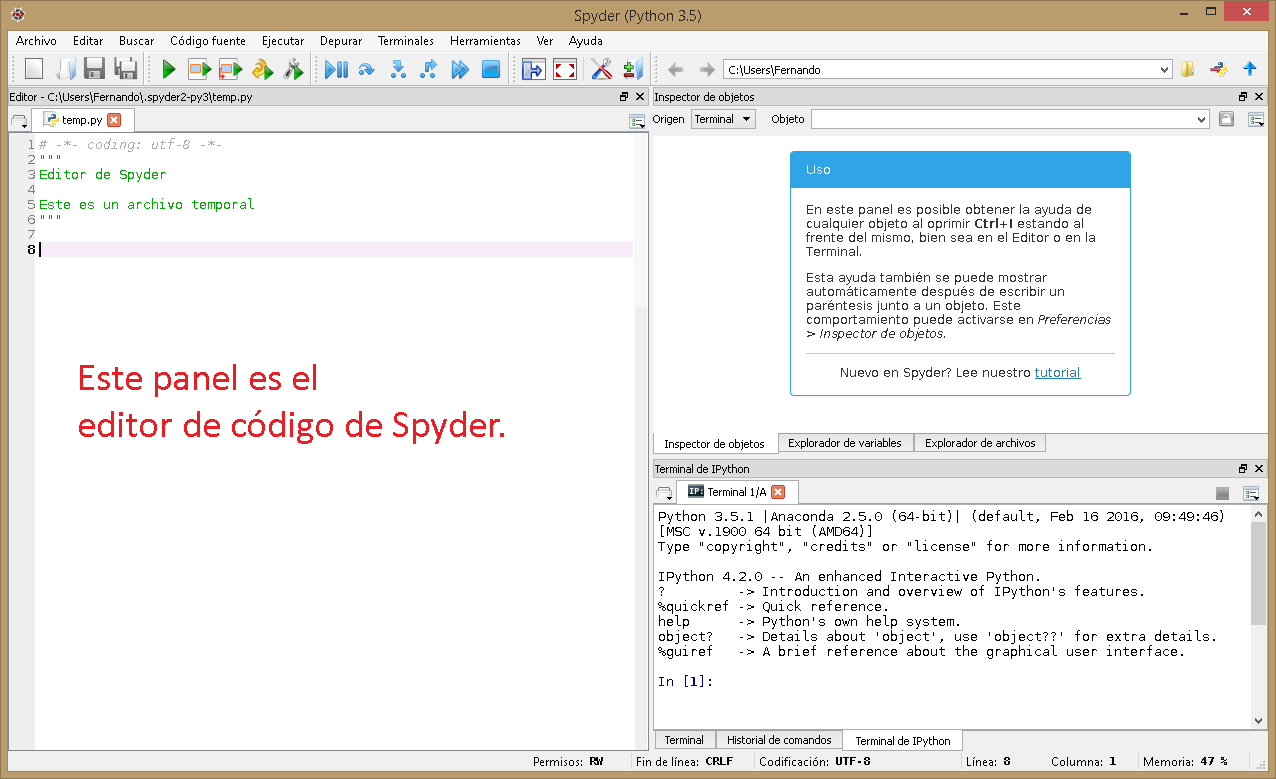
\includegraphics[width=15cm]{../fig/Tut-02-py-23-PanelEditorSpyder-2.png}
\end{center}

Verás que el panel del editor contiene en la parte superior algunas líneas de texto (que pueden ser distintas de las que aparecen aquí). No te preocupes por ellas, porque no van a interferir en nuestro trabajo. Este panel se comporta en muchos sentidos como un editor de texto, al estilo del {\em Bloc de Notas} de Windows. Pero como irás viendo, es un editor de texto especialmente preparado para el trabajo con Python. 

Para empezar a trabajar con el Editor de Código, haz click en ese panel y asegúrate de que el cursor esté situado por debajo de las líneas del principio. A continuación escribe esta línea de código:
\begin{knitrout}
\definecolor{shadecolor}{rgb}{0.969, 0.969, 0.969}\color{fgcolor}\begin{kframe}
\begin{alltt}
import math as m
\end{alltt}
\end{kframe}
\end{knitrout}
En este momento deberías ver algo así en el Editor de código:
\begin{center}
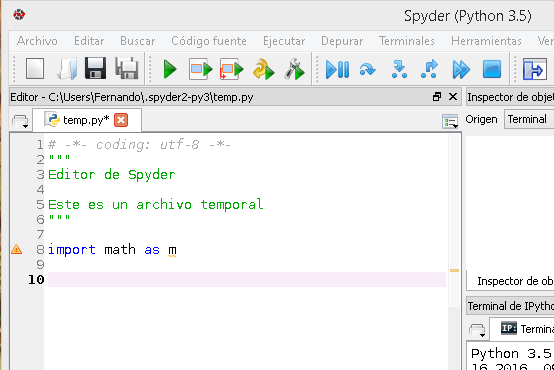
\includegraphics[width=14cm]{../fig/Tut-02-py-24-EditorSpyder01.png}
\end{center}
Algunas observaciones:
\begin{itemize}
  \item Por el momento no te preocupes por el triángulo amarillo de advertencia que ha aparecido a la izquierda de esa línea. Esos mensajes de Spyder te serán muy útiles más adelante, pero por ahora lo mejor es ignorarlo (salvo que sea de color rojo, en cuyo caso probablemente significa que has copiado mal el código).
  \item Si te fijas verás que las palabras {\tt import} y {\tt as} aparecen en color azul, mientras que {\tt math} y {\tt m} son de color negro. La diferencia es que las dos primeras son palabras reservadas del lenguaje Python, mientras que {\tt math} y {\tt m} son identificadores, como los nombres de variables. Este {\em código de colores} es el segundo ejemplo que vemos de la forma en la que el Editor de Texto nos ayuda al escribir código en Python (el primer ejemplo fue el triángulo amarillo de advertencia). 
\end{itemize}
Hemos dicho que este panel de Spyder es parecido al {\em Bloc de Notas}. Pero es un bloc de notas que incluye estas características especiales, como el {\sf reconocimiento de sintaxis} para Python. Eso significa que se usan colores, tipos de letra, etc. para destacar la estructura del programa y ayudarnos así en nuestro trabajo. Además, como iremos viendo, el Editor de Código vigila que nuestro programa cumpla unas normas básicas de sintaxis Python, ahorrándonos los errores más evidentes (de esa forma Spyder se asegura de que cuando cometamos errores, al menos sean errores interesantes...)

Todavía hay más. Vamos a añadir una línea de código más a ese panel, justo debajo de la anterior. Queremos añadir una línea para calcular la raíz cuadrada de 2. Ya sabes que para eso podemos usar:
\begin{knitrout}
\definecolor{shadecolor}{rgb}{0.969, 0.969, 0.969}\color{fgcolor}\begin{kframe}
\begin{alltt}
\hlkwd{m.sqrt}\hlstd{(}\hlnum{2}\hlstd{)}
\end{alltt}
\end{kframe}
\end{knitrout}
Cuando empieces a teclear esta línea, justo después de teclear el punto que contiene esa línea te encontrarás con que aparece esto:
\begin{center}
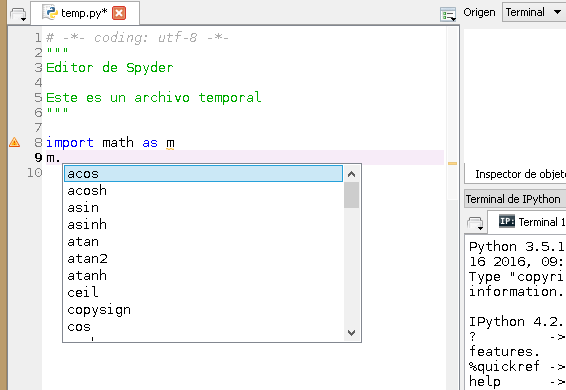
\includegraphics[width=12cm]{../fig/Tut-02-py-24-EditorSpyder02.png}
\end{center}
¿Qué está ocurriendo?
\begin{itemize}
  \item Spyder ha visto la primera línea y sabe que vamos a usar {\tt m} como alias del módulo {\tt math}.
  \item Por lo tanto, al escribir {\tt m.} Spyder sabe que nos vamos a referir a una función de ese módulo, y nos muestra una lista con todas las funciones que contiene (lo cuál puede ser muy útil si sólo recuerdas aproximadamente el nombre de la función). 
\end{itemize}
En cualquier caso no te preocupes, sigue escribiendo esa línea de código hasta el final. Cuando escribas el primer paréntesis verás que Spyder añade el segundo paréntesis (para que no nos olvidemos, como sucede a menudo con expresiones complejas con paréntesis anidados) y retorcede una posición para que podamos seguir escribiendo cómodamente dentro de ese par de paréntesis. Añade el 2 hasta obtener:
\begin{center}
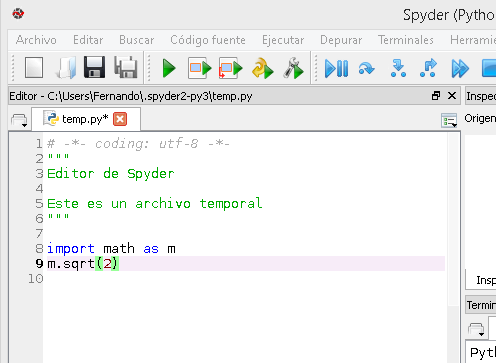
\includegraphics[width=12cm]{../fig/Tut-02-py-24-EditorSpyder03.png}
\end{center}
Un detalle más: al situar el cursor a la izquierda del segundo paréntesis verás que Spyder {\em ilumina o resalta} en color verde los dos paréntesis de la pareja, de nuevo como ayuda visual para que sea fácil identificar que paréntesis izquierdo corresponde a cada paréntesis derecho.

Ahora empieza la parte divertida. Usando el teclado o el ratón, selecciona las dos líneas de código que has tecleado, como aparecen en esta figura:
\begin{center}
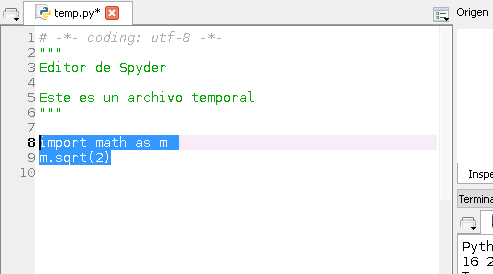
\includegraphics[width=12cm]{../fig/Tut-02-py-24-EditorSpyder04.png}
\end{center}

Y ahora, en el menú {\em Ejecutar (o Run)} de Spyder (los nombres de opciones varían ligeramente entre Windows, Mac y Linux), selecciona la opción {\em Ejecutar la Selección (Run selection)} o simplemente, pulsa la tecla de función {\tt F9}. Al hacerlo fíjate en lo que sucede en la terminal de IPython:
\begin{center}
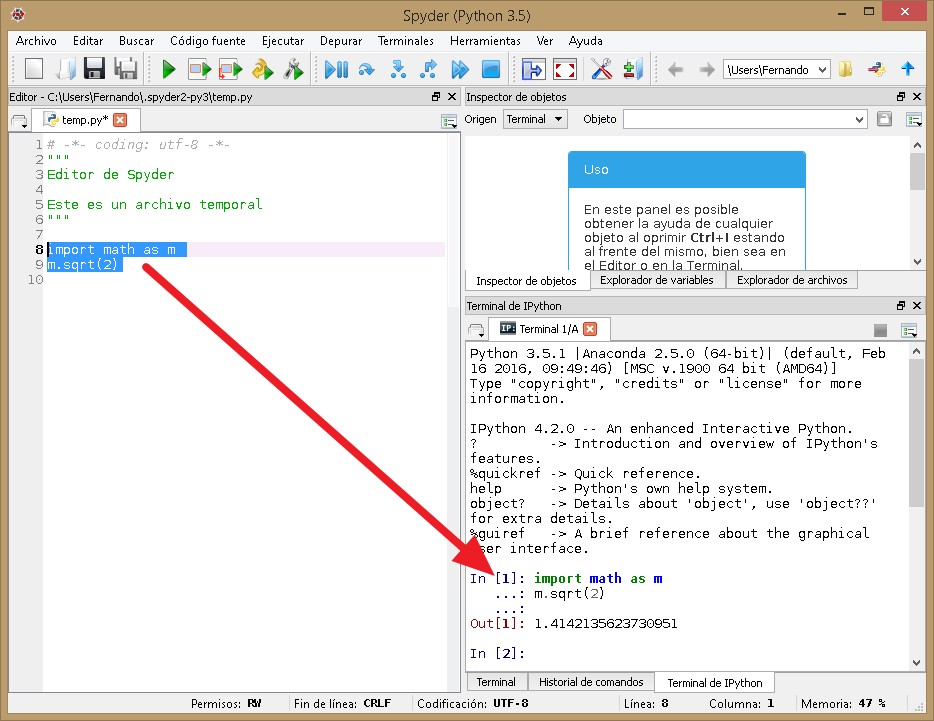
\includegraphics[width=10cm]{../fig/Tut-02-py-24-EditorSpyder05.png}
\end{center}
En efecto, Python ha ejecutado esas líneas de código y se muestra el resultado. De hecho no hace falta ejecutar las dos líneas a la vez. Si sitúas de nuevo 
el cursor en la primera línea, sin seleccionarla por completo (basta con que el cursor esté en esa línea) y pulsas {\tt F9} (o usas el menú): 
\begin{center}
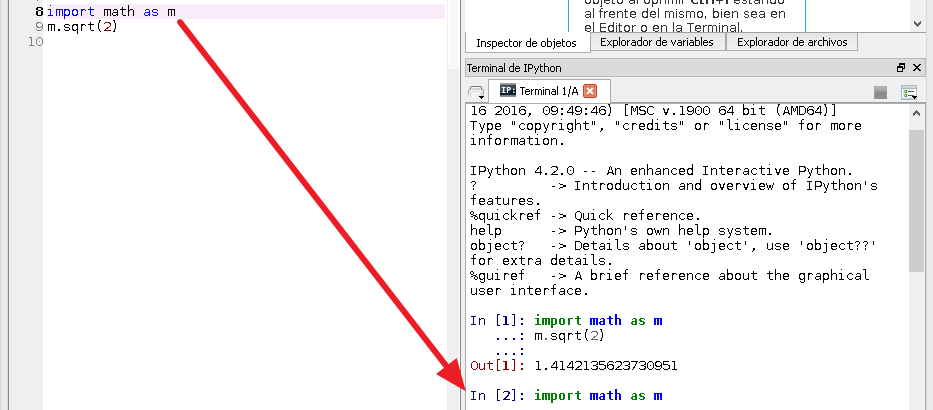
\includegraphics[width=10cm]{../fig/Tut-02-py-24-EditorSpyder06.png}
\end{center}
Como puedes comprobar sólo se ejecuta esa línea. Haz lo mismo con la segunda línea para ver cómo funciona. 

Esta conexión entre esos dos paneles de Spyder, el Editor de Textos por un lado y la Terminal de Ipython por otro, nos va a servir para trabajar con mucha comodidad: normalmente escribiremos el código de nuestros programas en el Editor de Textos. De esa forma aprovechamos toda la ayuda que nos presta, y de la que ya hemos empezado a ver algunas muestras. Y cada vez que queramos ver cómo funciona una parte de nuestro código, usamos esa conexión para ejecutarlo. Aunque al principio te puede costar añadir este nuevo ingrediente a la mezcla, pronto te acostumbrarás y verás que resulta una forma sencilla de trabajar. 

Un experimento más. Añade una nueva línea al {\em Editor de Código}, con esta asignación:
\begin{knitrout}
\definecolor{shadecolor}{rgb}{0.969, 0.969, 0.969}\color{fgcolor}\begin{kframe}
\begin{alltt}
\hlstd{a} \hlkwb{=} \hlnum{2}
\end{alltt}
\end{kframe}
\end{knitrout}
y ejecúta esa línea usando {\tt F9}. Como era de esperar, la línea se ejecuta en la terminal (y no hay línea de salida). Ahora haz clic con el ratón {\bf en la terminal} y ejecuta:
\begin{knitrout}
\definecolor{shadecolor}{rgb}{0.969, 0.969, 0.969}\color{fgcolor}\begin{kframe}
\begin{alltt}
\hlkwd{print}\hlstd{(a} \hlopt{+} \hlnum{1}\hlstd{)}
\end{alltt}
\end{kframe}
\end{knitrout}
Como resultado obtendrás 3, claro. No hay ninguna sorpresa en esto, y sólo queremos reforzar la idea de que el {\em Editor de Código} y la {\em Terminal} están realmente conectados a través del mecanismo que hemos visto. Por supuesto, esta última línea de código (con {\tt print}) que hemos escrito en la {\em Terminal} no aparece por ningún sitio en el {\em Editor de Código}. Más adelante veremos la utilidad de esto.

\subsection{Ficheros de comandos Python.}
\label{tut02:subsec:ficherosComandosPython}

El {\em Editor de Código} nos va a servir para escribir programas Python. Esos programas se almacenan en ficheros de texto simple, con extensión {\tt .py} para identificarlos fácilmente y para que nuestro ordenador sepa qué aplicación utilizar para abrir esos ficheros. En principio, puedes abrir y modificar uno de esos ficheros con cualquier editor de texto, como el {\tt Bloc de Notas} de Windows. Pero, como ya hemos visto, es mejor usar el editor de código que incorpora Spyder, porque así disponemos de reconocimiento de la sintaxis de Python y de otras ayudas para el trabajo de programación. 

Esos ficheros de código Python se pueden intercambiar fácilmente con otros usuarios, permitiéndonos así compartir programas útiles. Para empezar a practicar el manejo de esos ficheros incluimos aquí como adjunto un fichero de código Python especialmente simple, que se limita a calcular y mostrar el volumen y área de una esfera cuyo radio se define mediante el valor de la variable {\tt r } que aparece en la segunda línea del código.

\begin{center}
\fichero{./code/Tut02-py-VolAreaEsfera.py}{Tut02-py-VolAreaEsfera.py}
\end{center}
y cuyo contenido se muestra a continuación:
\begin{knitrout}
\definecolor{shadecolor}{rgb}{0.969, 0.969, 0.969}\color{fgcolor}\begin{kframe}
\begin{verbatim}
import math as m 

r = 2

V = (4 / 3) * m.pi * r**3

S = 4  * m.pi * r**2

print("El volumen de la esfera es ", V)

print("y su superficie es ", S)
\end{verbatim}
\end{kframe}
\end{knitrout}
Como ves, hemos dejado líneas en blanco entre cada dos líneas de código. No es necesario hacer esto y en cualquier caso al ejecutar el programa Python va a ignorar esas líneas vacías. Pero a menudo puede ser útil como recurso visual, para hacer más legible el programa. Ya veremos más recomendaciones de estilo, necesarias para convertirnos en programadores con buenas prácticas del oficio.

Vamos a abrir este fichero en el {\em Editor de Código} de Spyder. Empieza por guardar ese fichero (recuerda usar el botón derecho del ratón para descargarlo del pdf) en tu directorio de trabajo. Es recomendable, una vez más, que cierres y vuelvas a abrir Spyder antes de continuar, para empezar el trabajo en un entorno limpio. Una vez hecho eso, usa el menú {\em Archivo} y la opción {\em Abrir} de Spyder. En la ventana que se abre (y que depende de tu sistema, Windows, Mac o Linux) navega hasta tu directorio de trabajo y selecciona el fichero {\tt Tut02-py-VolAreaEsfera.py} que contiene nuestro programa. Spyder lo abrirá en una pestaña del {\tt Editor de código} , y verás algo como lo que se muestra en esta figura:
\begin{center}
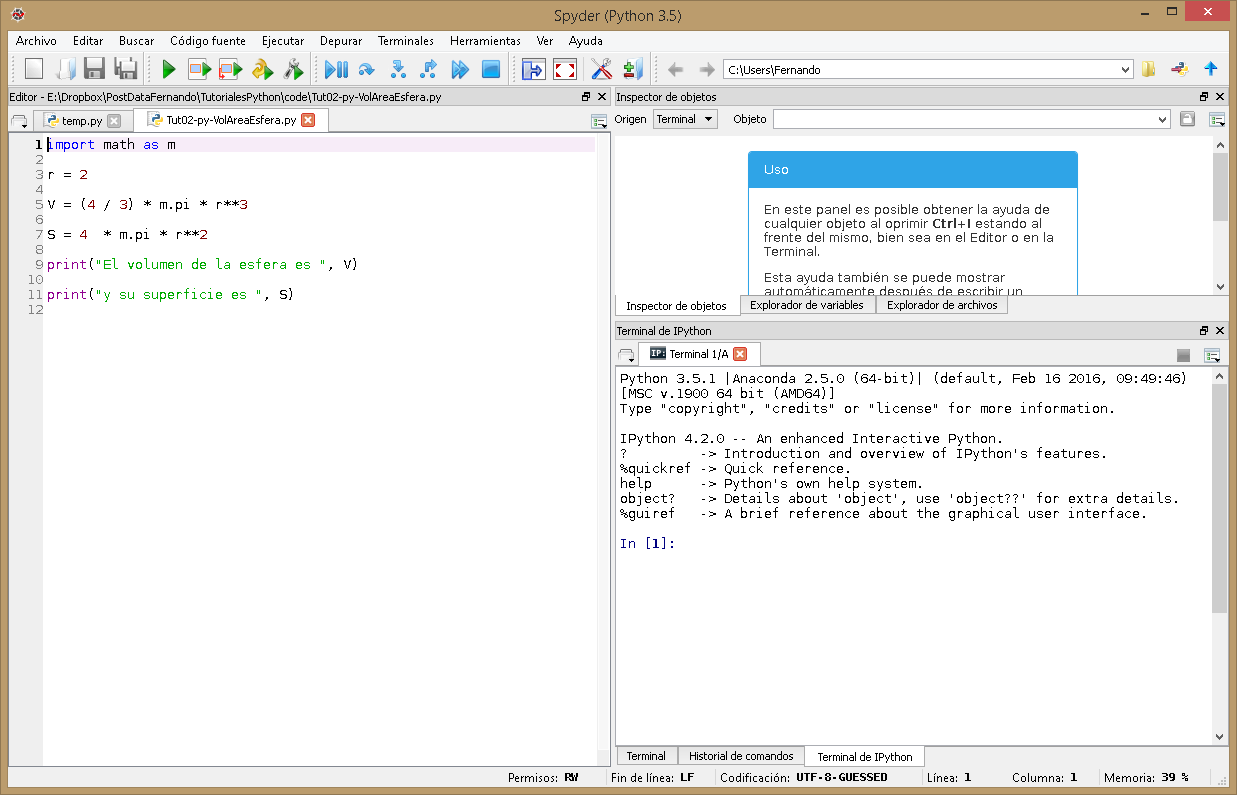
\includegraphics[width=13cm]{../fig/Tut-02-py-25-FicheroEnEditorSpyder.png}
\end{center}
Como puedes ver, Spyder está aplicando reconocimiento de sintaxis Python al fichero y usando colores para ayudarnos a identificar los componentes de ese programa. Una observación antes de seguir: la primera pestaña normalmente contendrá el fichero temporal {\tt temp.py} que Spyder crea siempre al comensar para almacenar el código que aún no hemos guardado en un fichero. Puedes hacer click en ella para revisar su contenido. Es posible que esa primera pestaña contenga aún código de nuestra sesión de trabajo previa. No te preocupes, no interferirá con lo que vamos a hacer. Vuelve a la pestaña que contiene el programa {\tt Tut02-py-VolAreaEsfera.py}.

Ya hemos visto antes que puedes ir ejecutando una por una las líneas de código que aparecen en el {\em Editor} (recuerda, basta con usar {\tt F9} con el cursor situado en la línea que quieres ejecutar). Pero en el caso de un programa completo como este, podemos ejecutar todo el código de una vez pulsando {\tt F5}. Al ser la primera vez que ejecutamos código, aparecerá un cuadro de diálogo como este:
\begin{center}
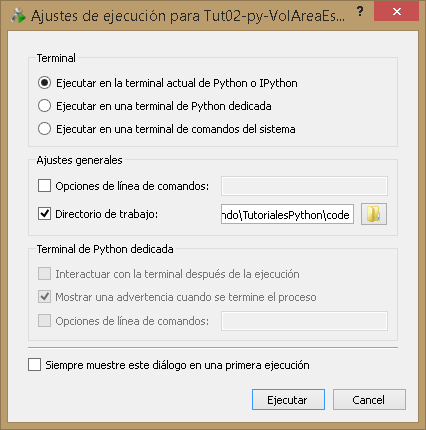
\includegraphics[width=7cm]{../fig/Tut-02-py-27-SpyderDialogoEjecucion}
\end{center}
Podemos aceptar todas las opciones por defecto, así que haz click en {\em Ejecutar} ({\em Run} si tu versión de Spyder está en inglés). En la {\em Terminal} aparecerá el resultado de la ejecución, como se ve en esta figura: 
\begin{center}
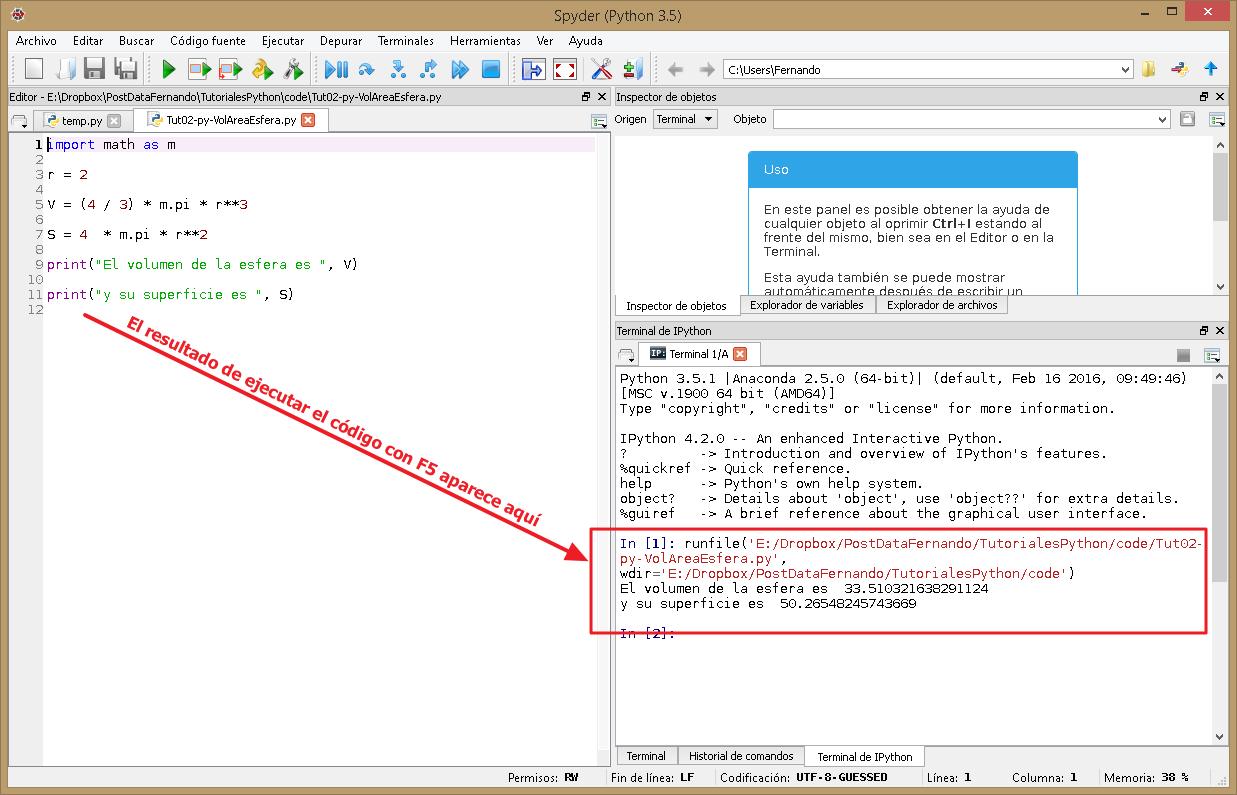
\includegraphics[width=14cm]{../fig/Tut-02-py-28-SpyderResultadoF5}
\end{center}
Verás  una clara diferencia con lo que sucedía cuando ejecutábamos el código línea a línea. Ahora, para ejecutar nuestro código Python ha usado una función llamada {\tt runfile} (con dos opciones, que corresponden al nombre del fichero de código y al nombre del directorio de trabajo). Y en la terminal no vemos las líneas de código que componen el programa, sino solamente la salida que produce ese código (mediante {\tt print}). 

Para ver más clara la diferencia, vamos a añadir una líne más al código en la que calculamos la relación entre el volumen y el área de la esfera. Es decir, añadimos esta línea de código justo al final del fichero:
\begin{knitrout}
\definecolor{shadecolor}{rgb}{0.969, 0.969, 0.969}\color{fgcolor}\begin{kframe}
\begin{alltt}
\hlstd{V} \hlopt{/} \hlstd{S}
\end{alltt}
\end{kframe}
\end{knitrout}
Después de añadir esa línea vuelve a pulsar {\tt F5} (al hacerlo, Spyder graba automáticamente el fichero de código con los cambios que hemos hecho). Como verás, en la terminal aparece de nuevo el resultado de ejecutar el código, pero no hay ningún cambio visible como respuesta a esa nueva línea. 
\begin{center}
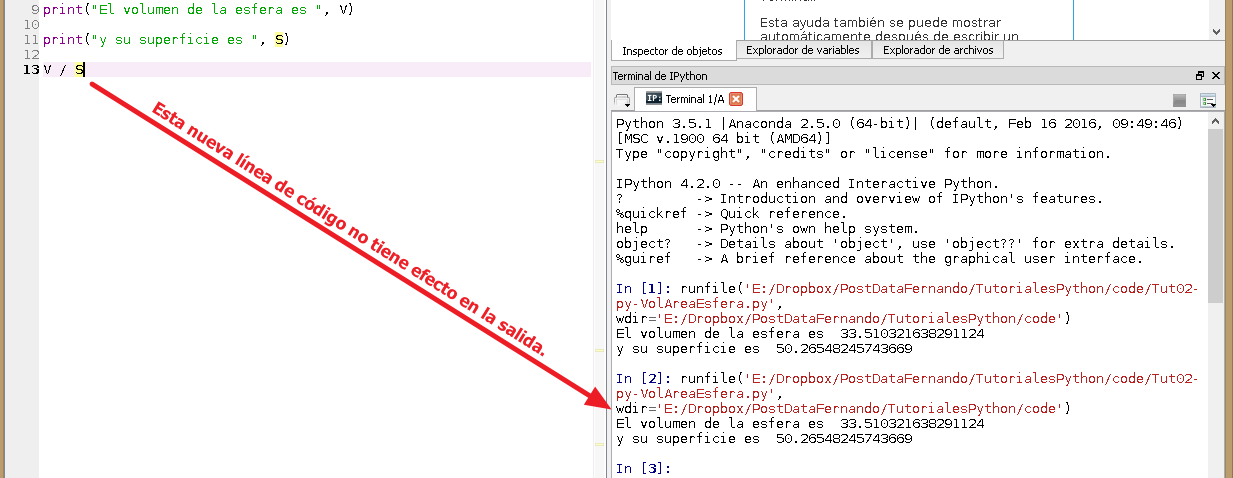
\includegraphics[width=15cm]{../fig/Tut-02-py-29-CodigoSinEfectoVisible.png}
\end{center}
Si ahora sitúas el cursor en esa última línea del {\em Editor de Código} y pulsas {\tt F9} (para ejecutar sólo esa línea) el resultado que verás en la terminal es:
\begin{knitrout}
\definecolor{shadecolor}{rgb}{0.969, 0.969, 0.969}\color{fgcolor}\begin{kframe}
\begin{alltt}
\hlstd{In [}\hlnum{3}\hlstd{]}\hlopt{:} \hlstd{V} \hlopt{/} \hlstd{S}
\hlstd{Out[}\hlnum{3}\hlstd{]}\hlopt{:} \hlnum{0.6666666666666666}
\end{alltt}
\end{kframe}
\end{knitrout}
La razón por la que sucede esto es que, tras ejecutar el programa, Python sabe ahora cuáles son los valores de {\tt V} y {\tt S}. Al ejecutar esa línea con {\tt F9}, usando lo que llamaremos {\sf modo interactivo}, Python se comporta como una calculadora que muestra el resultado de esa operación.

Vamos a insistir en la idea. Cambia esa línea para que sea:
\begin{knitrout}
\definecolor{shadecolor}{rgb}{0.969, 0.969, 0.969}\color{fgcolor}\begin{kframe}
\begin{alltt}
\hlstd{RazonVS} \hlkwb{=} \hlstd{V} \hlopt{/} \hlstd{S}
\end{alltt}
\end{kframe}
\end{knitrout}
y vuelve a usar {\tt F5}. Como antes, no hay efecto {\em visible} de esa última línea de código. Pero el código se ha ejecutado. Si te sitúas en la terminal, escribes {\tt RazonVS} y pulsas {\em Enter} para ejecutarlo, verás que Python sabe cuál es el valor, porque lo ha calculado al ejecutar el programa.
\begin{center}
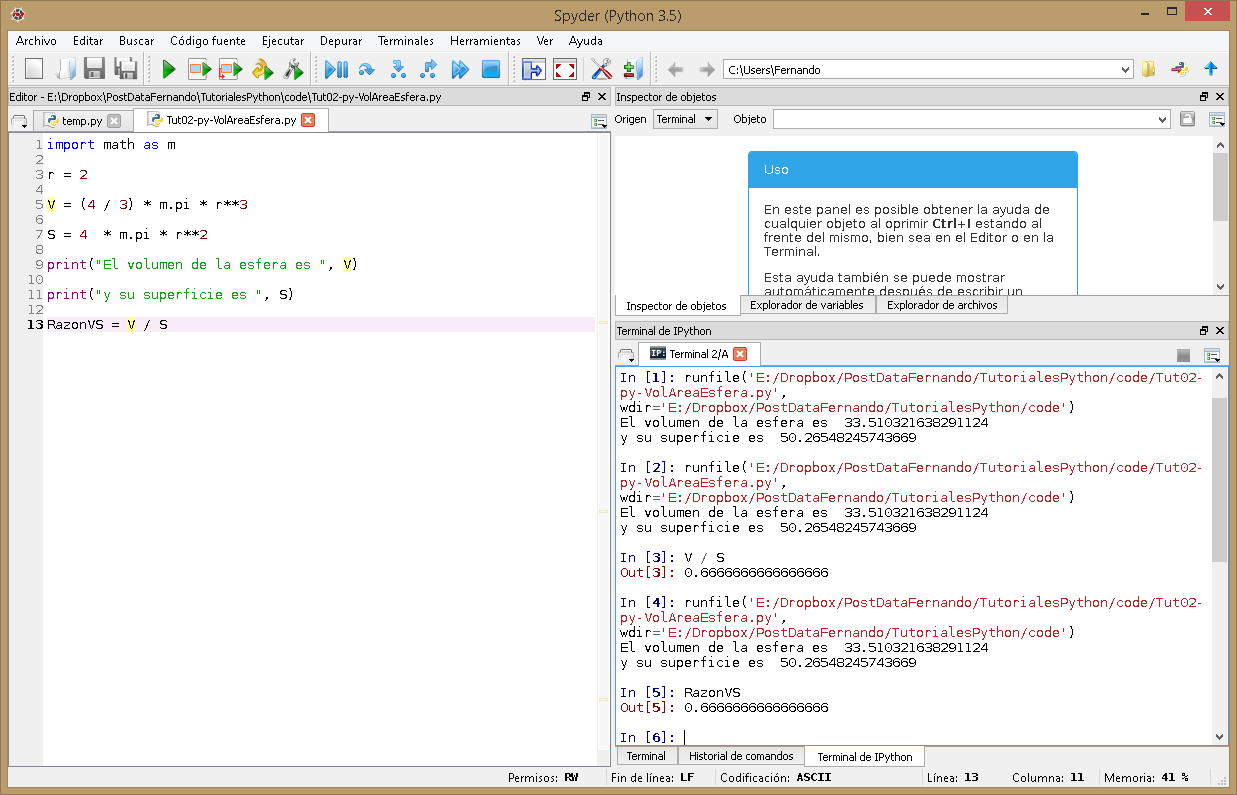
\includegraphics[width=15cm]{../fig/Tut-02-py-30-EditorVsTerminal}
\end{center}
Como sucede con todas las novedades que estamos aprendiendo en este tutorial, al principio te puede costar acostumbrarte al vínculo entre la {\em Terminal} y el {\em Editor de Código} de Spyder. Pero con la práctica y a medida que avancemos por estos tutoriales, todo irá quedando más claro y llegarás a dominar estas herramientas. A partir de ahora verás que nuestra atención se desplaza cada vez más hacia el {\em Editor de Código}, com olugar natural en el que escribir con comodidad el código Python. 

\subsubsection*{Un comentario sobre otros editores de texto.}

Hemos repetido varias veces que muchos programadores prefieren trabajar con otras herramientas, en lugar de usar un entorno de desarrollo integrado como Spyder.  ¿Por qué? Una de las posibles razones es que a menudo un programador utiliza más de un lenguaje de programación en su trabajo. Es común usar una combinación de Python con R, o con C++, JavaScript, etc. Y los entronos de desarrollo como Spyder a menudo son especialistas en un lenguaje, pero no se llevan igual de bien con los otros. Por esa razón a veces los programadores prefieren trabajar directamente con editores de texto, similares al {\em Bloc de Notas} pero más potentes, que reconocen la sintaxis de muchos lenguajes de programación. En el Tutorial00 hemos mencionado varios de ellos. Por ejemplo: Notepad++ en Windows, TextWrangler en Mac OS X, gedit en Linux. En cualquier caso los ficheros de texto simple son una parte esencial del trabajo en Computación y un buen editor de texto simple es un aliado importante para cualquier programador o científico. Así que, aunque sigas usando Spyder para 
programar en Python, te recomendamos que te familiarices con uno de ellos. 


%%%%%%%%%%%%%%%%%%%%%%%%%%%%%%%%%%%%%%%%%%%%%%%%%%%%%%%%%%%%%%%%%%%%%%%%%%%%%%%%%%%%%%%%%%%
\section{Bucles {\tt for}.}
\label{tut02py:sec:BuclesFor}
%%%%%%%%%%%%%%%%%%%%%%%%%%%%%%%%%%%%%%%%%%%%%%%%%%%%%%%%%%%%%%%%%%%%%%%%%%%%%%%%%%%%%%%%%%%

Como hemos dicho, una de las operaciones básicas en computación consiste en aplicar una operación a cada uno de los elementos de una lista. Nos hemos encontrado ya con una situación en la que queríamos hacer esto, al tratar de calcular la varianza poblacional de la lista {\tt edades}. Recuerda que la lista es:
{\small
\begin{knitrout}
\definecolor{shadecolor}{rgb}{0.969, 0.969, 0.969}\color{fgcolor}\begin{kframe}
\begin{alltt}
22, 21, 18, 19, 17, 21, 18, 20, 17, 18, 17, 22, 20, 19, 18, 19,
18, 22, 20, 19, 22, 18, 20, 21, 20
\end{alltt}
\end{kframe}
\end{knitrout}
}
y que ya hemos calculado su media, que es $\frac{486}{25}$. La definción de la varianza poblacional de una lista $x_1, x_2, \ldots, x_n$ es:
\[
Var(x) = \dfrac{(x_1 - \bar x)^2 + (x_2 - \bar x)^2 + \cdots + (x_n - \bar x)^2}{n}
\]
Y para calcular el numerador de esa fórmula empezaremos calculando esta lista de valores (los cuadrados de las desviaciones):
\[
(x_1 - \bar x)^2, (x_2 - \bar x)^2, \ldots , (x_n - \bar x)^2
\]
Después de obtener esa lista, tendremos que calcular su suma y dividir por $n$. Pero estos últimos dos pasos ya hemos aprendido a hacerlos en Python usando las funciones {\tt sum} y {\tt len}. Así que el paso clave es la construcción de la lista de cuadrados de las desviaciones. 

En esta sección vamos a aprender cuál es la solución de Python para este tipo de {\sf problemas iterativos}. Insistimos: problemas en los que se trata de ir recorriendo uno tras otro los elementos de una lista (o de algún otro tipo de conjunto o estructura de datos), aplicando una cierta operación en cada posición de la lista. Este tipo de problemas son uno de los ingredientes básicos de la Computación. Por eso, todos los lenguajes de programación incluyen instrucciones para realizar esas tareas iterativas. Y si no conoces ningún otro lenguaje de programación, lo que aprendas aquí para Python te facilitará en el futuro el aprendizaje de ese tipo de instrucciones en otros lenguajes. 

Para ponernos las cosas más sencillas desde el principio, vamos a empezar con un problema más sencillo, pero que contiene el ingrediente clave que necesitaremos para resolver el problema del cálculo la varianza. El problema es este:
\begin{quote}
Imagínate que tenemos la lista de números del 1 al 10 y queremos calcular el cuadrado de cada uno de esos números.
\end{quote}
La frase que acabamos de escribir es una descripción del 















En palabras podemos describir lo que queremos hacer así:

\begin{knitrout}
\definecolor{shadecolor}{rgb}{1, 0.851, 0.702}\color{fgcolor}\begin{kframe}
\begin{alltt}
Suponemos que partimos de una lista llamada edades y que 
la variable edadMedia contiene su media.

Creamos una lista vacía llamada cuadradosDesviaciones.
Para cada edad de la lista edades:
    Restamos edadMedia de esa edad, elevamos el \hlkwd{resultado} (desviacion) al cuadrado 
    y añadimos ese cuadrado a la lista cuadradosDesviaciones.

Una vez hecho esto, dividimos la suma de lista cuadradosDesviaciones 
entre \hlkwd{n} (la longitud de la lista edades) y guardamos el resultado en 
la variable varianzaEdades.
\end{alltt}
\end{kframe}
\end{knitrout}
Esta descripción en palabras de lo que vamos a hacer es un ejemplo de {\sf pseudocódigo}. El pseudocódigo es un lenguaje especial, a medio camino entre el lenguaje natural que hablamos y los lenguajes formales de programación como Python. El pseudocódigo muestra la estructura del algoritmo (método) que vamos a usar, pero en general nos ahorra los detalles más técnicos del lenguaje de programación concreto (Python en este caso). Las ventajas de usar pseudocódigo son, entre otras:
\begin{enumerate}
  \item  El programador puede usar el pseudocódigo cuando está diseñando un programa, para concentrarse en la estructura del programa. Los detalles se ajustan después. Para un programador experimentado, el paso del pseudocódigo al código es una labor de {\em traducción} relativamente sencilla.

  \item Por esa misma capacidad de abstracción, el pseudocódigo puede utilizarse para traducir un algoritmo a distintos lenguajes de programación.
  
  \item Para otros programadores, distintos del autor del programa, el pseudocódigo sirve como guía para facilitar la comprensión del código. Y por la parte que nos toca como programadores, podemos asegurarte que, pasado un cierto tiempo no muy largo, el propio autor del programa se alegrará enormemente de haber dejado escrito el pseudocódigo que guió el diseño del programa. Todos hemos pasado por la experiencia frustrante de no entender el código que nosotros mismos hemos escrito hace un tiempo. 
\end{enumerate}

En el caso que nos ocupa, hemos dividido el pseudocódigo en tres bloques, separados por líneas en blanco. El primer y último bloques describen operaciones que ya sabemos hacer en Python. El bloque central es que incluye la novedad de una operación que debemos repetir para cada elemento de la lista {\tt edades}. Esta es la parte que vamos a aprender a traducir a Python mediante una construcción llmada {\sf bucle for} (en inglés, {\em for loop})). Primero veamos esa traducción a Python que, como verás, se corresponde muy fáilmente con el pseudocódigo que hemos escrito. El programa adjunto contiene esta traducción, y su código se muestra a continuación:

\begin{center}
\fichero{./code/Tut02-py-VarianzaEdades.py}{Tut02-py-VarianzaEdades.py}
\end{center}
\begin{knitrout}
\definecolor{shadecolor}{rgb}{0.969, 0.969, 0.969}\color{fgcolor}\begin{kframe}
\begin{verbatim}
edades = [22, 21, 18, 19, 17, 21, 18, 20, 17, 18, 17, 22, 20, 19, 18, 19, 18, 22, 
          20, 19, 22, 18, 20, 21, 20]
edadMedia = sum(edades) / len(edades)

cuadradosDesviaciones = []
for edad in edades:
  cuadradosDesviaciones = cuadradosDesviaciones + [(edad - edadMedia)**2]

varianzaEdades = sum(cuadradosDesviaciones) / len(cuadradosDesviaciones)
print(varianzaEdades)
\end{verbatim}
\end{kframe}
\end{knitrout}
Hemos insertado líneas en blanco en el código del programa, para dividirlo en tres bloques que coinciden con las tres partes de nuesgro pseudocódigo. Antes de analizar la estructura del programa y el funcionamiento del bucle for vamos a ejecutarlo para comprobar que funciona. Como de costumbre, al comenzar una nueva sesión de trabajo es recomendable que cierres y vuelvas a abrir Spyder o al menos que uses \verb&%reset& y \verb&%clear&
en la terminal. Después descarga y guarda ese fichero en tu directorio de trabajo para a continuación abrirlo en el {\em Editor de Código} de Spyder. Deberías ver algo así (se muestra la versión para Mac OS de Spyder):
\begin{center}
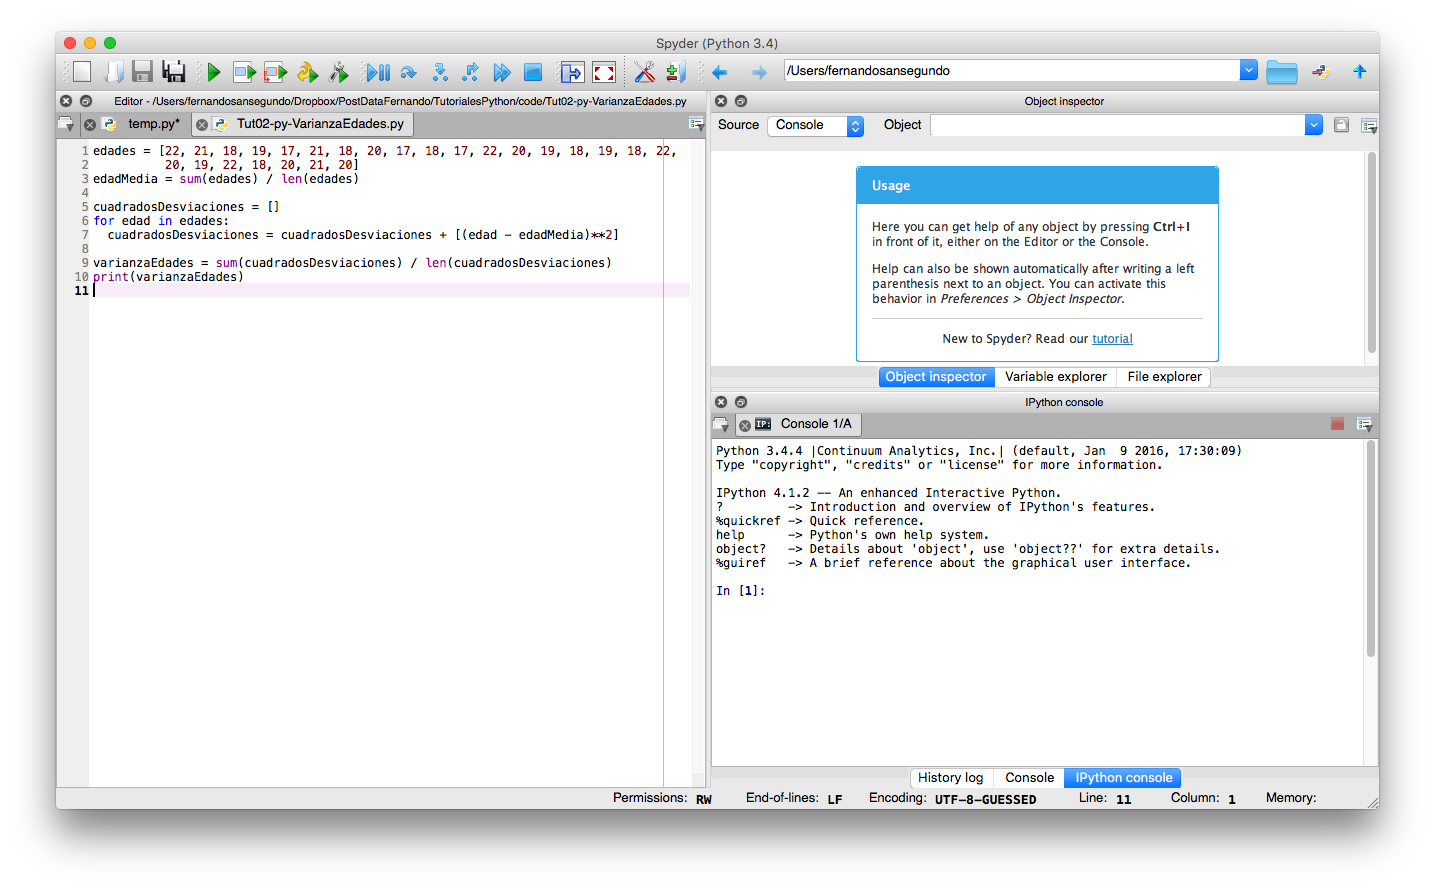
\includegraphics[width=16cm]{../fig/Tut-02-py-31-programaVarEdades.png}
\end{center}
Una vez hecho esto, basta con que ejecutes el programa en Spyder pulsando {\tt F5}. El resultado que deberías ver aparecer en la {\em Terminal} es:
\begin{knitrout}
\definecolor{shadecolor}{rgb}{0.969, 0.969, 0.969}\color{fgcolor}\begin{kframe}
\begin{alltt}
\hlnum{2.646400000000001}
\end{alltt}
\end{kframe}
\end{knitrout}
El resultado exacto es $2.6464$, pero el redondeo en las operaciones hace que Python lo muestre así.  Te recomiendo que antes de seguir compruebes este resultado, por ejemplo usando la hoja de cálculo Calc como aprendimos a hacer en el Tutorial01 (recuerda usar {\tt VARP}, no {\tt VAR}).

Una vez visto que el código hace lo que esperábamos vamos a analizarlo en detalle. El bloque inicial en el que calculamos la media es ya conocido, así que vamos a fijarnos en las tres líneas del segudo bloque, que contienen el bucle for.
\begin{knitrout}
\definecolor{shadecolor}{rgb}{0.969, 0.969, 0.969}\color{fgcolor}\begin{kframe}
\begin{verbatim}
cuadradosDesviaciones = []
for edad in edades:
  cuadradosDesviaciones = cuadradosDesviaciones + [(edad - edadMedia)**2]
\end{verbatim}
\end{kframe}
\end{knitrout}
Vamos con el análisis línea a línea de este bloque:
\begin{enumerate}
\item En la primera línea simplemente hemos creado una lista vacía, llamada {\tt cuadradosDesviaciones}. Esta línea en realidad no forma parte del bucle for, que empieza en la segunda línea. Pero es muy frecuente que antes del bucle necesitemos una o más {\sf líneas de inicialización}, como esta, en las que creamos los objetos que vamos a necesitar en el bucle o asignamos valores a algunas variables.

\item La segunda línea
\begin{knitrout}
\definecolor{shadecolor}{rgb}{0.969, 0.969, 0.969}\color{fgcolor}\begin{kframe}
\begin{verbatim}
for edad in edades:
\end{verbatim}
\end{kframe}
\end{knitrout}
es la {\sf línea de cabecera del bucle for}. La variable {\tt edad} que aparece aquí es una {\sf variable auxiliar}, cuyo papel consiste en ir recorriendo uno a uno los valores de la lista {\tt edades}. Podríamos haber usado cualquier otro nombre para esa variable auxiliar (volveremos sobre esto enseguida). Un {\bf detalle muy importante} es que esa línea termina con dos puntos. Si los olvidas, Python señalará un error en esa línea.

\item La tercera línea de código
\begin{knitrout}
\definecolor{shadecolor}{rgb}{0.969, 0.969, 0.969}\color{fgcolor}\begin{kframe}
\begin{verbatim}
  cuadradosDesviaciones = cuadradosDesviaciones + [(edad - edadMedia)**2]
\end{verbatim}
\end{kframe}
\end{knitrout}
forma el {\sf cuerpo del bucle for}. En este caso es una única línea, pero en general el cuerpo del bucle lo formarán varias líneas (veremos ejemplos pronto). Esta línea se ejecuta una vez para cada uno de los elementos de {\tt edades}. Cada una de esas ejecuciones se denomina una {\sf iteración} del bucle. En la primera iteración del bucle, la variable auxiliar {\tt edad} toma el primer valor de la lista {\tt edades} (es decir, 22). En la segunda iteración, {\tt edad} toma el segundo valor de la lista {\tt edades} (que es 21), etc. Y la operación que hacemos en cada iteración con el valor {\tt edad} es la que hemos descrito en el pseudocódigo: restamos la media a la edad, elevamos al cuadrado y concatenamos el resultado al final de la lista {\tt cuadradosDesviaciones}. Un detalle técnico: fíjate en que hemos rodeado esa operación con corchetes para convertir el resultado en una lista (de un único elemento) y así poder usar {\tt +} para concatenarla.

Fíjate en {\bf otro detalle muy importante}. Esa línea de código está {\sf indentada}; es decir, que hemos usado espacios en blanco al principio de la línea para desplazarla a la derecha con respecto a la línea anterior. En Python todas las líneas que forman el cuerpo de un bucle for deben estar indentadas con respecto a la línea de cabecera. De hecho esa indentación es la forma que usa Python para saber donde empieza y donde termina el cuerpo del código (en otros lenguajes el cuerpo del bucle se encierra entre llaves).

\end{enumerate}

El tercer bloque de código del programa:
\begin{knitrout}
\definecolor{shadecolor}{rgb}{0.969, 0.969, 0.969}\color{fgcolor}\begin{kframe}
\begin{verbatim}
varianzaEdades = sum(cuadradosDesviaciones) / len(cuadradosDesviaciones)
print(varianzaEdades)
\end{verbatim}
\end{kframe}
\end{knitrout}
ya no forma parte del cuerpo del bucle for y por esa razón las líneas que lo forman no están indentadas. Estas líneas se ejecutan tras terminar la iteraciones del bucle o, como diremos a menudo, {\em al salir del bucle}. En ellas simplemente sumamos la lista {\tt cuadradosDesviaciones}, dividimos la suma entre {\tt n}, asignamos el resultado a la variable {\tt varianzaEdades} y usamos {\tt print} para mostrar el resultado.

Para mejorar nuestra comprensión del funcionamiento del bucle for vamos a hacer un ejercicio:
\begin{ejercicio}
\label{tut02:ejercicio15}
\quad
\begin{enumerate}
\item Prueba a eliminar los dos puntos del final de la línea de cabecera del bucle y ejecuta otra vez todo el bloque de código. ¿Cuál es el mensaje de error?

\item Vamos a ejecutar otra vez el bucle for, pero cambiando el nombre de la variable auxiliar {\tt edad} así:
\begin{knitrout}
\definecolor{shadecolor}{rgb}{0.969, 0.969, 0.969}\color{fgcolor}\begin{kframe}
\begin{alltt}
cuadradosDesviaciones = []
for x in edades:
  cuadradosDesviaciones = cuadradosDesviaciones + [(x - edadMedia)**2]
\end{alltt}
\end{kframe}
\end{knitrout}
Fíjate en que hemos cambiado por {\tt x} las dos apariciones de {\tt edad}. ¿Hay algún cambio en el resultado final? Prueba a usar otro nombre cualquiera y repite este apartado con ese nombre. Aunque este ejercicio muestra que puedes usar cualquier nombre (que no hayas usado para otra cosa, claro) siemrpe es conveniente que el nombre sea descriptivo del papel qu ejuega la variable.

\item {\bf Importante:} Prueba a indentar la dos últimas líneas del programa y elimina la línea en blanco para hacerlas parte del cuerpo del bucle. Es decir, convierte el programa en este otro:

¿Qué sucede ahora al ejecutar el código? ¿Cuántos valores aparecen? ¿Reconoces el último de ellos? 
\end{enumerate}
\quad\\
%Solución en la página \pageref{tut02:ejercicio15:sol}.
\qed
\end{ejercicio}

\subsubsection*{Otra forma de hacerlo: comprensión de listas.}
\label{tut02:subsubsec:comprensionListas}

Los bucles for como los que hemos visto en el apartado anterior existen en muchos otros lenguajes de programación, con prácticamente la misma estructura. Sólo varían los detalles de formato propios de cada lenguaje. Pero Python dispone además de una forma alternativa dehacer esto; es decir, de ejecutar la misma colección de operaciones sobre los elementos de una lista. El cálculo de las desviaciones al cuadrado de cada elemento de {\tt edades} se puede obtener de esta forma alternativa así:
\begin{knitrout}
\definecolor{shadecolor}{rgb}{0.969, 0.969, 0.969}\color{fgcolor}\begin{kframe}
\begin{alltt}
edadesCuadrado = [(edad - **2 for edad in edades]
\hlkwd{print}(edadesCuadrado)
\end{alltt}
\end{kframe}
\end{knitrout}
En la terminal de IPython el resultado es:
\begin{knitrout}
\definecolor{shadecolor}{rgb}{0.969, 0.969, 0.969}\color{fgcolor}\begin{kframe}
\begin{alltt}
In [5]: edadesCuadrado = [edad**2 for edad in edades]

In [6]: \hlkwd{print}(edadesCuadrado)
[484, 441, 324, 361, 289, 441, 324, 400, 289, 324, 289, 484, 400, 361,
324, 361, 324, 484, 400, 361, 484, 324, 400, 441, 400]
\end{alltt}
\end{kframe}
\end{knitrout}

Como ves no hay ninguna diferencia con el resultado del bucle for.

Esta segunda forma de trabajar se denomina {\sf comprensión de listas}, una traducción decepcionantemente literal del nombre en inglés {\em list comprehension} (que ya es, en sí mismo, desafortunado).

La comprensión de lista en nuestro ejemplo se refiere concretamente a la expresión entre corchetes:
\begin{knitrout}
\definecolor{shadecolor}{rgb}{0.969, 0.969, 0.969}\color{fgcolor}\begin{kframe}
\begin{alltt}
[edad**2 for edad in edades]
\end{alltt}
\end{kframe}
\end{knitrout}
Esta expresión se puede ver como una receta para fabricar una lista: es como si le dijeramos a Python:
\begin{knitrout}
\definecolor{shadecolor}{rgb}{0.969, 0.969, 0.969}\color{fgcolor}\begin{kframe}
\begin{alltt}
[haz esta operación para cada elemento de la lista]
\end{alltt}
\end{kframe}
\end{knitrout}
Y de nuevo, como sucedía en el bucle for, la variable auxiliar puede recibir cualquier nombre y el resultado es el mismo:
\begin{knitrout}
\definecolor{shadecolor}{rgb}{0.969, 0.969, 0.969}\color{fgcolor}\begin{kframe}
\begin{alltt}
[item**2 for item in edades]
\end{alltt}
\end{kframe}
\end{knitrout}
Puesto que en inglés {\em un elemento de la lista} se suele escribir {\em an item in the list}, es frecuente que los programadores de Python usen {\tt item} como nombre para la variable auxiliar cuando no hay un nombre preferible. Recuerda en cualquier caso lo que hemos dicho sobre la conveniencia de usar nombres de variable esclarecedores.

\begin{ejercicio}
\label{tut02:ejercicio16}
\quad
\begin{enumerate}
\item Ejecuta este código para comprobar que en efecto produce el mismo resultado.
\item Escribe una comprensión de lista que reste a cada elemento de {\tt edades} la media aritmética y eleve al cuadrado la cantidad resultante y úsala para calcular la varianza poblacional. Comparala con la que hemos obtenido antes.
\end{enumerate}
\quad\\
%Solución en la página \pageref{tut02:ejercicio16:sol}.
\qed
\end{ejercicio}

%' \subsubsection*{Y todavía una forma más: Numpy y aritmética vectorial.}
%' \label{tut02:subsubsec:numpyAritmeticaVectorial}
%'
%' <<eval=FALSE, purl=FALSE>>=
%' import numpy as np
%' edades_np = np.array(edades)
%' edades_np
%' edades_np + 1
%' edades_np**2
%' @

\subsubsection*{Ordenación de una lista: in situ vs externa.}
\label{tut02:subsubsec:ordenacionLista}

Cerramos esta primera visita a las listas de Python analizando una operación que también vamos a usar con frecuencia: la ordenación de los elementos de una lista. El caso más habitual es el de la ordenación de una lista de números. Por ejemplo, dada esta lista no ordenada de números:



\begin{knitrout}
\definecolor{shadecolor}{rgb}{0.969, 0.969, 0.969}\color{fgcolor}\begin{kframe}
\begin{alltt}
numeros = [10, 8, 43, 7, 24, 7, 31, 45, 1, 3, 20, 14, 12, 44, 13, 20, 33, 7, 29, 5]
\end{alltt}
\end{kframe}
\end{knitrout}

podemos ordenarla fácilmente con la función {\tt sorted}. En IPython:

\begin{knitrout}
\definecolor{shadecolor}{rgb}{0.969, 0.969, 0.969}\color{fgcolor}\begin{kframe}
\begin{alltt}
In [1]: numeros = [10, 8, 43, 7, 24, 7, 31, 45, 1, 3, 20, 14, 12, 44, 13, 20, 33, 7, 29, 5]

In [2]: \hlkwd{print}(\hlkwd{sorted}(numeros))
[1, 3, 5, 7, 7, 7, 8, 10, 12, 13, 14, 20, 20, 24, 29, 31, 33, 43, 44, 45]
\end{alltt}
\end{kframe}
\end{knitrout}

Si lo que queremos es ordenarlos de mayor a menor basta con añadir un argumento a la función:
\begin{knitrout}
\definecolor{shadecolor}{rgb}{0.969, 0.969, 0.969}\color{fgcolor}\begin{kframe}
\begin{alltt}
In [3]: \hlkwd{print}(\hlkwd{sorted}(numeros, reverse=True))
[45, 44, 43, 33, 31, 29, 24, 20, 20, 14, 13, 12, 10, 8, 7, 7, 7, 5, 3, 1]
\end{alltt}
\end{kframe}
\end{knitrout}
El valor {\tt True} es uno de los dos {\sf valores booleanos} de Python, {\tt True/False} (cierto/falso) sobre los que volveremos más adelante. De momento puedes pensar en el argumento  {\sf reverse=True} como un interruptor que permite activar o desactivar el orden decreciente en la función {\tt sorted}. Iremos viendo que muchas otras funciones de Python tienen argumentos booleanos como este que sirven precisamente para conmutar entre dos posibles comportamientos de la función.

Fíjate en que el proceso de ordenación no ha afectado a la lista original, que sigue desordenada:
\begin{knitrout}
\definecolor{shadecolor}{rgb}{0.969, 0.969, 0.969}\color{fgcolor}\begin{kframe}
\begin{alltt}
In [4]: \hlkwd{print}(numeros)
[10, 8, 43, 7, 24, 7, 31, 45, 1, 3, 20, 14, 12, 44, 13, 20, 33, 7, 29, 5]
\end{alltt}
\end{kframe}
\end{knitrout}
Por eso decimos que la función {\tt sorted} hace una ordenación {\sf externa}. En otras ocasiones preferiremos que la lista ordenada remplace a la lista original. Hay dos formas de hacer esto y es probable que ya hayas adivinado cuál es la primera. Bastaría con hacer:
\begin{knitrout}
\definecolor{shadecolor}{rgb}{0.969, 0.969, 0.969}\color{fgcolor}\begin{kframe}
\begin{alltt}
\hlstd{numeros} \hlkwb{=} \hlkwd{sorted}\hlstd{(numeros)}
\end{alltt}
\end{kframe}
\end{knitrout}
Pero no vamos a hacer esto, porque queremos aprovechar para mostrarte el segundo procedimiento y de paso aprender un poco más de Python. El segundo método consiste en ejecutar el comando:
\begin{knitrout}
\definecolor{shadecolor}{rgb}{0.969, 0.969, 0.969}\color{fgcolor}\begin{kframe}
\begin{alltt}
\hlkwd{numeros.sort}\hlstd{()}
\end{alltt}
\end{kframe}
\end{knitrout}
Vamos a hacer esto en IPython, mostrando la lista {\tt numeros} antes y después de ejecutar ese comando:
\begin{knitrout}
\definecolor{shadecolor}{rgb}{0.969, 0.969, 0.969}\color{fgcolor}\begin{kframe}
\begin{alltt}
In [5]: \hlkwd{print}(numeros)
[10, 8, 43, 7, 24, 7, 31, 45, 1, 3, 20, 14, 12, 44, 13, 20, 33, 7, 29, 5]

In [6]: \hlkwd{numeros.sort}()

In [7]: \hlkwd{print}(numeros)
[1, 3, 5, 7, 7, 7, 8, 10, 12, 13, 14, 20, 20, 24, 29, 31, 33, 43, 44, 45]
\end{alltt}
\end{kframe}
\end{knitrout}
El resultado es el que queríamos: la lista ordenada remplaza a la original. Esto es lo que se conoce como ordenación {\em in situ}. En general usamos ese término cuando una modificación de un objeto ocupa el lugar del objeto original.

Pero el otro aspecto interesante de este segunda manera de ordenar la lista  es el propio formato del comando que hemos usado. Python es un lenguaje {\sf orientado a objetos}. Aunque no vamos a entrar en la discusión técnica de lo que eso significa en Computación, sí queremos que conozcas algo del lenguaje. Todas las construcciones que vamos viendo: variables, listas, funciones y muchas otras que veremos son {\sf objetos}. Y cada objeto de Python tiene un serie de {\sf métodos} asociados. Los métodos representan acciones que podemos llevar a cabo usando ese objeto. Por ejemplo, cualquier objeto de clase {\em lista} (como  {\tt numeros}) tiene asociado el método {\tt sort} que permite ordenar {\em in situ} ese objeto. La forma general de invocar un método en Python es un comando de la forma:
\begin{knitrout}
\definecolor{shadecolor}{rgb}{0.969, 0.969, 0.969}\color{fgcolor}\begin{kframe}
\begin{alltt}
\hlkwd{objeto.metodo}\hlstd{(argumentos_del_metodo)}
\end{alltt}
\end{kframe}
\end{knitrout}
El comando {\tt numeros.sort()} que hemos visto es un ejemplo de esta construcción, aunque en ese caso el método {\tt sort} se invoca sin argumentos. También podíamos haber hecho ordenación {\em in situ} descendente:
\begin{knitrout}
\definecolor{shadecolor}{rgb}{0.969, 0.969, 0.969}\color{fgcolor}\begin{kframe}
\begin{alltt}
In [9]: \hlkwd{numeros.sort}(reverse=True)

In [10]: \hlkwd{print}(numeros)
[45, 44, 43, 33, 31, 29, 24, 20, 20, 14, 13, 12, 10, 8, 7, 7, 7, 5, 3, 1]
\end{alltt}
\end{kframe}
\end{knitrout}
y en este caso el método {\tt sort} si tiene un argumento que es: {\tt reverse=True}. A lo largo del curso nos vamos a encontrar muchas veces con dos formas de ejecutar acciones en Python. La primera que vimos es de la forma:
\begin{knitrout}
\definecolor{shadecolor}{rgb}{0.969, 0.969, 0.969}\color{fgcolor}\begin{kframe}
\begin{alltt}
\hlkwd{funcion}\hlstd{(argumentos)}
\end{alltt}
\end{kframe}
\end{knitrout}
y la que estamos presentando ahora, que es:
\begin{knitrout}
\definecolor{shadecolor}{rgb}{0.969, 0.969, 0.969}\color{fgcolor}\begin{kframe}
\begin{alltt}
\hlkwd{objeto.metodo}\hlstd{(argumentos_del_metodo)}
\end{alltt}
\end{kframe}
\end{knitrout}
Ambas son comunes a casi todos los lenguajes de programación modernos. En el próximo apartado vamos a ver otro ejemplo.

\subsubsection*{De nuevo la función {\tt print}. Textos con formato.}
\label{tut02:subsubsec:funcionPrintTextosFormato}

Ya dijimos al presentarla que la función {\tt print} nos proporciona un mecanismo de control mucho más fino sobre la forma de mostrar los resultados de nuestro código. En este apartado vamos a ver como combinar la función {\tt print} con las variables de tipo cadena y los bucles y rangos para dar un salto cualitativo en nuestra capacidad de expresarnos mediante Python.

Empezamos con un ejemplo sencillo. Fíjate en lo que sucede al ejecutar este código en IPython:
\begin{knitrout}
\definecolor{shadecolor}{rgb}{0.969, 0.969, 0.969}\color{fgcolor}\begin{kframe}
\begin{alltt}
In [1]: a = 7

In [2]: \hlkwd{print}(\hlstr{"El valor de la variable a es  \{0\}"}\hlkwd{.format}(a))
El valor de la variable a es  7
\end{alltt}
\end{kframe}
\end{knitrout}
El resultado es que la función {\tt print} produce como salida la cadena de caracteres, pero al hacerlo sustituye la parte {\tt\{0\}} de esa cadena  con el valor de la variable {\tt a}. ¿Y cómo sabe Python cuál es la variable que debe usar como sustituto de {\tt\{0\}}? Se lo hemos indicado mediante el método {\tt format} aplicado a esa cadena de caracteres.
El mecanismo puede resultar un poco lioso al principio, pero con la práctica resulta más natural y es en cualquier caso una herramienta de presentación muy potente, como tendremos ocasión de comprobar en estos tutoriales. Veamos otros dos ejemplos que introducen novedades interesantes:
\begin{knitrout}
\definecolor{shadecolor}{rgb}{0.969, 0.969, 0.969}\color{fgcolor}\begin{kframe}
\begin{alltt}
In [1]: tiempo = 7

In [2]: espacio = 123

In [3]: velocidad = espacio / tiempo

In [4]: \hlkwd{print}(\hlstr{"Hemos recorrido \{0\} metros en \{1\} segundos."}\hlkwd{.format}(espacio, tiempo))
Hemos recorrido 123 metros en 7 segundos.

In [5]: \hlkwd{print}(\hlstr{"Por lo tanto la velocidad ha sido igual a \{0:5.2f\} m/s"}\hlkwd{.format}(velocidad))
Por lo tanto la velocidad ha sido igual a 17.57 m/s
\end{alltt}
\end{kframe}
\end{knitrout}
El primer uso de la función {\tt print} es muy parecido al ejemplo anterior. La novedad es que aparecen dos variables en vez de una, y por tanto hemos usado {\tt\{0\}} y {\tt\{1\}} para indicarle a {\tt print} cuál es la variable que debe sustituir en cada posición (recuerda siempre que Python cuenta desde 0). Después el método {\tt format} le proporciona a {\tt print} esas variables, que se usan en el orden en el que aparecen como argumentos de {\tt format}.

Todas las variables que hemos usado en los ejemplos previos eran de tipo {\tt int}. En cambio, la  segunda llamada a {\tt print} de este ejemplo utiliza sólo una variable, pero esa variable es de tipo {\tt float}.  Además, las instrucciones que usamos para pedirle a Python que sustituya el valor de esa variable son más complicadas: hemos usado {\tt\{0:5.2f\}}. ¿Qué significa esto? La expresión entre llaves tiene dos partes, separadas por los dos puntos. La primera parte es simplemente el número de orden de la variable para el caso en que haya más de una y se corresponde, como hemos visto, con el orden en el que aparecerán enumeradas las variables en la llamada a {\tt format}. En este caso aparece un $0$, porque sólo hay que sustituir la variable {\tt velocidad}. La parte que sigue a los dos puntos {\tt 5.2f} es nueva. Empecemos por lo más fácil: la letra {\tt f} le indica a Python que se trata de sustituir una variable de tipo {\tt float}. Una vez aclarado eso, el símbolo {\tt 5.2} significa: {\em ``usa 5 espacios, y muestra dos decimales después de la coma''}. Vamos a hacer una modificación en esos valores para ver el efecto:
\begin{knitrout}
\definecolor{shadecolor}{rgb}{0.969, 0.969, 0.969}\color{fgcolor}\begin{kframe}
\begin{alltt}
In [6]: \hlkwd{print}(\hlstr{"Por lo tanto la velocidad ha sido igual a \{0:15.4f\} m/s"}\hlkwd{.format}(velocidad))
Por lo tanto la velocidad ha sido igual a         17.5714 m/s
\end{alltt}
\end{kframe}
\end{knitrout}
Fíjate en que al usar {\tt 15.4f} ahora aparecen cuatro cifras decimales después de la coma. Además ese espacio en blanco que ha aparecido antes del valor de la variable se debe a que le hemos pedido a Python que use 15 espacios para mostrar el valor de la variable. Y puesto que no necesitaba tantos, una parte de ellos están en blanco. Más adelante veremos que esto puede ser muy útil para dar un formato visual conveniente a nuestros resultados; por ejemplo al imprimir una tabla de valores, en la que queremos controlar la anchura de cada columna. Lo veremos a continuación.

\subsubsection*{Cómo imprimir una tabla de valores.}

La comprensión de listas, como hemos visto, es un proceso iterativo que sirve para fabricar una lista elemento a elemento. Por ejemplo, podemos usarla para fabricar una lista que represente una tabla de valores. Imagínate que vas a viajar en breve al Reino Unido y que tu moneda local es el euro. Puesto que allí usan la libra esterlina, puede resultar conveniente fabricar una tabla de conversión de precios en libras a precios en euros, que te permita por ejemplo saber si te están cobrando un precio exorbitante por esa pinta de cerveza. En el momento de escribir este tutorial, a comienzos del año 2016, el tipo de cambio es:\\

{\em Una libra equivale a 1.3164 euros.}\\

Vamos a fabricar una tabla que convierta los precios en libras, de media libra en media libra, desde 0.5 hasta 10 libras. Enseguida verás que son 20 valores. Así que podemos fabricar los valores en libras usando {\tt range(1:21)} y la comprensión de listas así:

\begin{knitrout}
\definecolor{shadecolor}{rgb}{0.969, 0.969, 0.969}\color{fgcolor}\begin{kframe}
\begin{alltt}
In [21]: libras = [valor * 0.5 for valor in \hlkwd{range}(1, 21)]

In [22]: \hlkwd{print}(libras)
[0.5, 1.0, 1.5, 2.0, 2.5, 3.0, 3.5, 4.0, 4.5, 5.0, 5.5, 6.0, 6.5, 7.0, 7.5,
8.0, 8.5, 9.0, 9.5, 10.0]
\end{alltt}
\end{kframe}
\end{knitrout}

Para convertir estas cantidades en libras a euros podemos usar otra vez una comprensión de lista. Vamos a introducir el tipo de cambio en una variable para que el código sea más fácil de entender y de modificar si el tipo de cambio sufre alguna alteración. :
\begin{knitrout}
\definecolor{shadecolor}{rgb}{0.969, 0.969, 0.969}\color{fgcolor}\begin{kframe}
\begin{alltt}
In [23]: tipoCambio = 1.3164

In [24]: euros = [valor * tipoCambio for valor in libras]

In [25]: \hlkwd{print}(euros)
[0.6582, 1.3164, 1.9746000000000001, 2.6328, 3.291, 3.9492000000000003, 4.6074,
5.2656, 5.9238, 6.582, 7.2402, 7.8984000000000005, 8.5566, 9.2148, 9.873, 10.5312,
11.189400000000001, 11.8476, 12.5058, 13.164]
\end{alltt}
\end{kframe}
\end{knitrout}
Podríamos conformarnos con este resultado. Pero el resultado no es muy cómodo, ni fácil de emplear en la práctica. Sería mucho mejor presentar nuestros resultados en una tabla. Y aquí tenemos una ocasión para comparar la comprensión de listas con el bucle {\tt for}. Como hemos visto, la comprensión de listas sirve para fabricar elementos iterativamente. Pero para fabricar la tabla queremos usar la función {\tt print} varias veces, una por cada línea. Y cuando se trata de {\em repetir acciones} a menudo es más natural expresar esa repetición  mediante un bucle {\tt for}. El código para fabricar la tabla podría ser este, que usa los formatos de {\tt print} que hemos visto antes:
\begin{knitrout}
\definecolor{shadecolor}{rgb}{0.969, 0.969, 0.969}\color{fgcolor}\begin{kframe}
\begin{alltt}
\hlkwd{print}(\hlstr{"Libras |  Euros"})
\hlkwd{print}(\hlstr{"-------|-------"})
for i in \hlkwd{range}(0, 20):
  \hlkwd{print}(\hlstr{" \{0:4.1f\}  |  \{1:5.2f\}"}\hlkwd{.format}(libras[i], euros[i]))
  \hlkwd{print}(\hlstr{"-------|-------"})
\end{alltt}
\end{kframe}
\end{knitrout}
El resultado de ejecutar este código en la terminal de IPython aparece en la
Tabla \ref{tut02:tabla:cambioLibrasEuros} (pág. \pageref{tut02:tabla:cambioLibrasEuros}).
\begin{table}[p]
\begin{center}
{\small
\begin{knitrout}
\definecolor{shadecolor}{rgb}{0.969, 0.969, 0.969}\color{fgcolor}\begin{kframe}
\begin{alltt}
Libras |  Euros
-------|-------
  0.5  |   0.66
-------|-------
  1.0  |   1.32
-------|-------
  1.5  |   1.97
-------|-------
  2.0  |   2.63
-------|-------
  2.5  |   3.29
-------|-------
  3.0  |   3.95
-------|-------
  3.5  |   4.61
-------|-------
  4.0  |   5.27
-------|-------
  4.5  |   5.92
-------|-------
  5.0  |   6.58
-------|-------
  5.5  |   7.24
-------|-------
  6.0  |   7.90
-------|-------
  6.5  |   8.56
-------|-------
  7.0  |   9.21
-------|-------
  7.5  |   9.87
-------|-------
  8.0  |  10.53
-------|-------
  8.5  |  11.19
-------|-------
  9.0  |  11.85
-------|-------
  9.5  |  12.51
-------|-------
 10.0  |  13.16
-------|-------
\end{alltt}
\end{kframe}
\end{knitrout}
}
\end{center}
\caption{Un ejemplo de tabla (cambio de libras esterlinas a euros).}
\label{tut02:tabla:cambioLibrasEuros}
\end{table}
El resultado es, desde luego, una tabla mucho más fácil de usar. Para conseguir ajustar el formato de esa tabla hemos tenido que hacer algo de ensayo y error con los espacios y el número de cifras decimales, pero son manipulaciones sencillas que tú mismo podrás experimentar en futuros ejemplos. Es cierto que ese formato no es impresionante, pero a partir de aquí, cualquier programador con unos conocimientos básicos de lenguajes para la Web (basta con los rudimentos de HTML y CSS) podría fácilmente escribir un programa que fabricaría una página web con esta tabla y el estilo que se desee (tipografías, colores, fondos, etc.) Es más, con apenas un poco más de aprendizaje de Python sería fácil diseñar un programa que cada cierto tiempo obtuviera la tasa de cambio libras/euros desde un servidor de internet y la usara para actualizar una página web con una tabla de cambios como esta. Tú mismo puedes imaginarte muchas otras aplicaciones similares. La presentación automatizada de resultados de análisis estadísticos mediante tablas o gráficos (a menudo el resultado se diseña en formato web) es una parte fundamental de la visualización que sirve de base a la comunicación científico-técnica actual.

\begin{ejercicio}
\label{tut02:ejercicio17}
\quad
¿Por qué al fabricar la lista {\tt libras} hemos usado {\tt range(1:21)}? Y teniendo esto en cuenta, ¿por qué en el bucle {\tt for} de la tabla hemos usado {\tt range(0:20)}?\quad\\
%Solución en la página \pageref{tut02:ejercicio17:sol}.
\qed
\end{ejercicio}
Este ejercicio apunta a una situación frecuente en programación, cuando queremos iterar {\em tomando como referencia una lista.} Algo así como: {\em ``repite esto tantas veces como elementos tiene una lista dada.''} La forma en la que hemos resuelto esto aquí es un poco artificiosa, veremos más adelante en el curso maneras mejores (más ``pythónicas'', como suele decirse) de abordar este problema.

\subsubsection*{Más formatos para {\tt print} y cifras significativas.}
\label{tut02:subsubsec:MasFormatosPrintCifrasSignificativas}

Para cerrar nuestro primer encuentro con las posibilidades que ofrece {\tt print} combinada el método {\tt format}, queremos añadir algunos comentarios sobre las opciones disponibles
para formatear valores numéricos. Hemos visto que podemos usar una construcción como {\tt\{0:5.2f\}} para indicarle a {\tt print} que queremos mostrar un número usando cinco espacios y dos cifras tras la coma. Existen otras construcciones similares, sustituyendo {\tt f} por otros códigos. Por ejemplo, si usamos {\tt\{0:5.2e\}} mira lo que se obtiene al pedirle a {\tt print} que nos muestre el valor de {\tt pi}:

\begin{knitrout}
\definecolor{shadecolor}{rgb}{0.969, 0.969, 0.969}\color{fgcolor}\begin{kframe}
\begin{alltt}
In [1]: import math as m

In [2]: \hlkwd{print}(\hlstr{"\{0:5.2e\}"}\hlkwd{.format}(m.pi))
3.14e+00
\end{alltt}
\end{kframe}
\end{knitrout}
El resultado es que el número se muestra en notación científica, y que {\tt 5.2} se utiliza para controlar tanto el número de posiciones que ocupa el número como el número de cifras tras la coma decimal. Estos otros ejemplos pueden aclarar cómo funciona esto. En cada versión hemos modificado cada componente del formato unidad a unidad para que puedas ver el efecto:
\begin{knitrout}
\definecolor{shadecolor}{rgb}{0.969, 0.969, 0.969}\color{fgcolor}\begin{kframe}
\begin{alltt}
In [3]: a = 163.5735

In [4]: \hlkwd{print}(\hlstr{"\{0:9.3e\}"}\hlkwd{.format}(a))
1.636e+02

In [5]: \hlkwd{print}(\hlstr{"\{0:10.3e\}"}\hlkwd{.format}(a))
 1.636e+02

In [6]: \hlkwd{print}(\hlstr{"\{0:10.4e\}"}\hlkwd{.format}(a))
1.6357e+02

In [7]: \hlkwd{print}(\hlstr{"\{0:11.4e\}"}\hlkwd{.format}(a))
 1.6357e+02
\end{alltt}
\end{kframe}
\end{knitrout}
Prueba con otros valores hasta convencerte de que entiendes lo que sucede. Aparte de {\tt f} y {\tt e}, existen muchos otros códigos de formato. La documentación oficial aparece en este enlace:
\begin{center}
\link{https://docs.python.org/2/library/string.html\#format-specification-mini-language}{https://docs.python.org/2/library/string.html\#format-specification-mini-language}
\end{center}
y si lo visitas podrás comprobar que apenas nos hemos asomado al tema de los formatos disponibles. Antes de seguir adelante sólo queremos añadir que el código de formato {\tt g} permite seleccionar el número de cifras significativas con las que se muestra un número.
Por ejemplo supongamos que, como en la Sección \ref{curso-cap01:sec:PrecisionExactitudCifrasSignificativas} del libro (pág. \pageref{curso-cap01:sec:PrecisionExactitudCifrasSignificativas}) queremos mostrar el número
\begin{knitrout}
\definecolor{shadecolor}{rgb}{0.969, 0.969, 0.969}\color{fgcolor}\begin{kframe}
\begin{alltt}
\hlstd{In [}\hlnum{1}\hlstd{]}\hlopt{:} \hlstd{a} \hlkwb{=} \hlnum{1.623698}
\end{alltt}
\end{kframe}
\end{knitrout}
con cuatro cifras significativas. Para ello basta con hacer:
\begin{knitrout}
\definecolor{shadecolor}{rgb}{0.969, 0.969, 0.969}\color{fgcolor}\begin{kframe}
\begin{alltt}
In [2]: \hlkwd{print}(\hlstr{"\{0:.4g\}"}\hlkwd{.format}(a))
1.624
\end{alltt}
\end{kframe}
\end{knitrout}
y se obtiene el resultado. Fíjate en que no es necesario indicar el número de espacios, Python lo asigan automáticamente si no lo incluimos. Siguiendo con el ejemplo más complicado de esa sección, para mostrar el número
\begin{knitrout}
\definecolor{shadecolor}{rgb}{0.969, 0.969, 0.969}\color{fgcolor}\begin{kframe}
\begin{alltt}
\hlstd{In [}\hlnum{3}\hlstd{]}\hlopt{:} \hlstd{b} \hlkwb{=} \hlnum{0.00337995246}
\end{alltt}
\end{kframe}
\end{knitrout}
con cinco cifras significativas hacemos:
\begin{knitrout}
\definecolor{shadecolor}{rgb}{0.969, 0.969, 0.969}\color{fgcolor}\begin{kframe}
\begin{alltt}
In [121]: \hlkwd{print}(\hlstr{"\{0:.5g\}"}\hlkwd{.format}(b))
0.00338
\end{alltt}
\end{kframe}
\end{knitrout}
En este caso conviene observar que Python, al igual que otros lenguajes, desgraciadamente no incluye ceros a la izquierda en este tipo de redondeos.

\section{Ficheros de comandos Python.}
\label{tut02:sec:ficherosComandosPython}

A medida que vamos empezando a escribir código más complejo en Python es muy probable que te estés empezando a dar cuenta de que la consola de IPython tiene ciertas limitaciones. Es una gran herramienta para hacer experimentos, para {\em explorar} datos e ideas y para cálculos rápidos. Pero si queremos desarrollar un proyecto más complejo y compartir nuestro trabajo con otras personas necesitamos otro tipo de soporte. Pero no te preocupes, es muy sencillo. Simplemente vamos a combinar nuestro trabajo en IPython con un editor de texto.  Aunque puedes usar cualquier editor, como el Bloc de Notas de Windows, es especialmente recomendable que uses un editor pensado para programar. Recuerda los ejemplos del Tutorial-00 (allí hay instrucciones de instalación): Notepad++ en Windows, Textwrangler en Mac y gedit en Linux.

Lo que vamos a hacer es trabajar con dos ventanas abiertas a la vez (tres, si cuentas el visor de pdf en el que lees este tutorial): en una tenemos nuestra terminal de IPython y en otra el editor de texto. La siguiente figura muestra el montaje en Windows 8.1:
\begin{center}
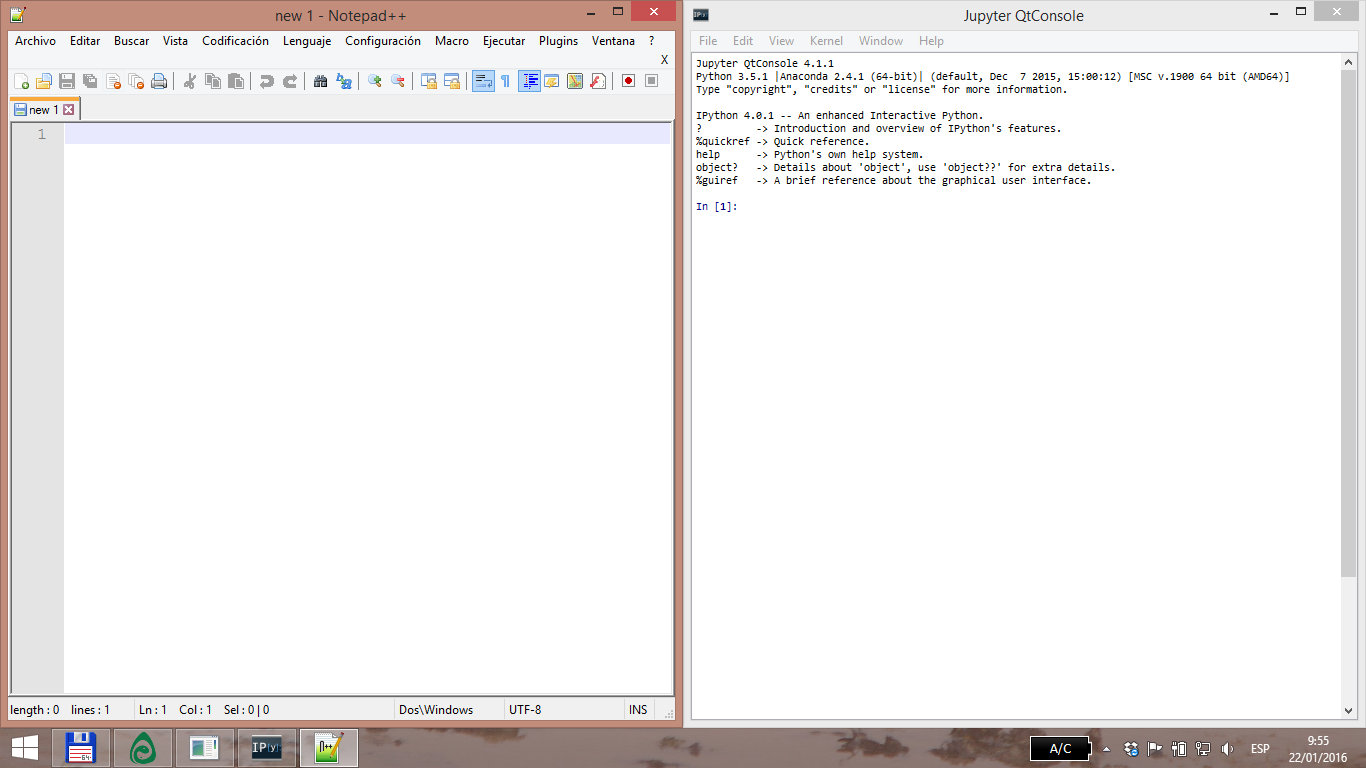
\includegraphics[height=8cm]{../fig/Tut02-py-06-EditorTextoJupyter.png}
\end{center}

Resumiendo el trabajo de los apartados anteriores vamos a crear un pequeño programa que a partir de una lista de números, como la lista {\tt edades} calcula la media aritmética, la varianza pobalacional y la desviación típica de esa lista. El código del programa es este:

\begin{knitrout}
\definecolor{shadecolor}{rgb}{0.969, 0.969, 0.969}\color{fgcolor}\begin{kframe}
\begin{alltt}
edades = [22, 21, 18, 19, 17, 21, 18, 20, 17, 18, 17, 22, 20, 19, 18, 19, 18, 22,
20, 19, 22, 18, 20, 21, 20]
\hlkwd{print}(\hlstr{"La lista de edades es:"})
\hlkwd{print}(edades)
mediaAritmetica = \hlkwd{sum}(edades) / \hlkwd{len}(eedades)
\hlkwd{print}(\hlstr{"La media aritmética es:"})
\hlkwd{print}(mediaAritmetica)
terminosVarianza = []
for edad in edades:
  terminosVarianza = terminosVarianza + [(edad - mediaAritmetica)**2]
varianzaPob = \hlkwd{sum}(terminosVarianza) / \hlkwd{len}(edades)
\hlkwd{print}(\hlstr{"La varianza poblacional es:"})
\hlkwd{print}(varianzaPob)
import math as m
\hlkwd{print}(\hlstr{"La desviación típica poblacional es:"})
\hlkwd{print}(\hlkwd{m.sqrt}(varianzaPob))
\end{alltt}
\end{kframe}
\end{knitrout}
Selecciona y copia todo este código y pégalo en el editor de texto. En el Tutorial-00 hemos creado una carpeta llamada {\tt code} dentro de tu directorio de trabajo. Desde el editor de texto guarda el programa en esa carpeta {\tt code} usando el nombre:
\begin{knitrout}
\definecolor{shadecolor}{rgb}{0.969, 0.969, 0.969}\color{fgcolor}\begin{kframe}
\begin{alltt}
Tut02-mediaVarianza-01.py
\end{alltt}
\end{kframe}
\end{knitrout}
El nombre podría ser cualquiera, pero es importante que la extensión sea {\tt py}. De esa forma el sistema reconoce este fichero como un fichero de texto que contiene código Python. De hecho, cuando lo guardes con esa extensión verás que el aspecto del texto cambia, de forma similar a lo que se ve en esta figura:
\begin{center}
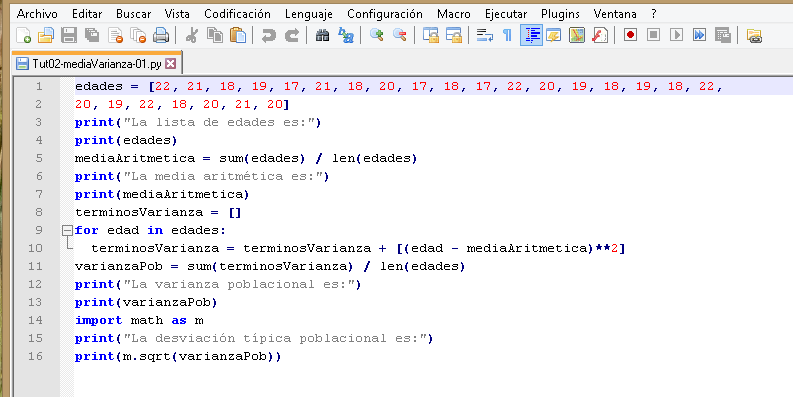
\includegraphics[width=15cm]{../fig/Tut02-py-07-EditorTextoSintaxis.png}
\end{center}
La razón es que los editores de texto orientados a la programación disponen de lo que se llama {\sf reconocimiento de sintaxis} para Python (y para muchos otros lenguajes de programación) y usan colores, tipos de letra, etc. para destacar la estructura del programa y ayudarnos así en nuestro trabajo. Aunque sólo fuera por eso, merece la pena hacer que el editor de texto forme parte de nuestras herramientas de programación en Python.

Ahora vamos a pasar a la ventana de IPython. Lo primero que tenemos que aprender a hacer es explicarle a IPython dónde está nuestro directorio de trabajo. En mi caso la carpeta de trabajo es una carpeta del {\em Escritorio} llamada {\em PostData}. Dentro de mi carpeta personal el {\em Escritorio} es la carpeta {\em Desktop}\footnote{Nota técnica sobre el {\em Escritorio para usuarios de Linux:} La carpeta {\em Desktop} del directorio de ususario representa al {\em Escritorio} tanto en sistemas Windows modernos como en Mac OS. En algunas versiones de Linux, por un afán de adaptación a mi juicio errado, esa carpeta se llama de hecho {\em Escritorio}. Si es tu caso, pero quieres poner la carpeta de trabajo en el Escritorio puedes abrir una consola de comandos, ir a tu carpeta ejecutando simplemente {\tt cd} y después ejecutar\\ {\tt ln -s Escritorio Desktop}\\ Eso creará un {\sf enlace simbólico} a tu escritorio llamado {\tt Desktop}, de manera que podrás usar ambos nombres indistintamente, sin duplicar ficheros.}. Para indicarle dónde está el fichero voya autilizar una nueva {\em función mágica} de IPython llamada \verb#%cd#
(del inglés {\em change directory}):
\begin{knitrout}
\definecolor{shadecolor}{rgb}{0.969, 0.969, 0.969}\color{fgcolor}\begin{kframe}
\begin{alltt}
%cd ~/Desktop/PostData/code
\end{alltt}
\end{kframe}
\end{knitrout}
Una aclaración: el símbolo \verb#~# que aparece aquí es una abreviatura que IPython interpreta como {\em la carpeta personal del usuario}. Tiene la ventaja de que funciona igual en los sistemas operativos Windows, Mac y Linux. Para obtener ese símbolo con el teclado usa AltGr + 4 en Windows/Linux y Alt+Ñ en Mac OS (sí, es una ñ mayúscula).

Si ejecuto la función mágica en mi terminal de IPython obtengo:
\begin{knitrout}
\definecolor{shadecolor}{rgb}{0.969, 0.969, 0.969}\color{fgcolor}\begin{kframe}
\begin{alltt}
In [1]: %cd ~/Desktop/PostData/code
/Users/fernando/Desktop/PostData/code
\end{alltt}
\end{kframe}
\end{knitrout}
donde como ves IPython ha sustituido \verb#~# por mi carpeta personal, que en esta máquina Windows se representa con {\tt /Users/fernando} (la primera barra inclinada {\tt /} representa aquí el {\sf directorio raíz} del sistema de ficheros de tu ordenador, la carpeta que contiene todas las demás carpetas).

Para comprobar que hemos llegado a la carpeta que contiene el fichero {\tt Tut02-mediaVarianza-01.py} vamos a usar otra {\em función mágica} de IPython. La función \verb#%ls#
sirve para mostrar el contenido de la carpeta activa, la que hemos seleccionado con \verb#%cd#.
Como sólo me interesan los ficheros de código Python usaré \verb#%ls *.py#
Así que si la ejecuto en IPython obtengo:

\begin{knitrout}
\definecolor{shadecolor}{rgb}{0.969, 0.969, 0.969}\color{fgcolor}\begin{kframe}
\begin{alltt}
In [2]: %ls *.py
Tut02-estadisticaDescriptiva.py  Tut02-mediaVarianza-02.py
Tut02-mediaVarianza-01.py
\end{alltt}
\end{kframe}
\end{knitrout}
Los detalles desde luego dependen de tu ordenador, sistema operativo y de la ubicación de tu carpeta de trabajo. Pero lo importante es que, en efecto, ahí aparece (entre otros) el fichero con nuestro código. Con eso estamos listos para usar la última de las funciones mágicas que vamos a necesitar en este apartado. La función \verb#%run#
ejecuta el programa contenido en un fichero de código Python que le proporcionamos como argumento (en Computación se suele traducir el inglés {\em run} por ejecutar, aunque también hemos oído una traducción más literal, {\em correr} el programa). En IPython sería:
\begin{knitrout}
\definecolor{shadecolor}{rgb}{0.969, 0.969, 0.969}\color{fgcolor}\begin{kframe}
\begin{alltt}
In [3]: %run Tut02-mediaVarianza-01.py
La lista de edades es:
[22, 21, 18, 19, 17, 21, 18, 20, 17, 18, 17, 22, 20, 19, 18, 19, 18, 22,
 20, 19, 22, 18, 20, 21, 20]
La media aritmética es:
19.44
La varianza poblacional es:
2.646400000000001
La desviación típica poblacional es:
1.6267759526130208
\end{alltt}
\end{kframe}
\end{knitrout}
Comprueba que esos valores son los que esperábamos. Fíjate en que al usar \verb#%run#
en IPython no aparecen las líneas de código Python del fichero {\tt Tut02-mediaVarianza-01.py} que estamos ejecutando, tan sólo aparece aquello que explícitamente hemos querido mostrar usando la función {\tt print}. Aunque de momento vamos a trabajar dentro de la consola de IPython, ese es el primer paso para que podamos escribir programas en Python que podrán utilizar usuarios que no sepan nada de programación. Al fin y al cabo todos nosotros usamos en nuestros ordenadores una gran cantidad de programas escritos en lenguajes de los que la mayoría de nosotros no sabemos nada.
Las ventajas de esta forma de trabajar a la vez con IPython y un editor de texto son múltiples: por un lado, el editor de texto ofrece un entorno mucho más cómodo que IPython a la hora de escribir nuestro código. No sólo
por el reconocimiento de sintaxis del que ya hemos hablado, sino porque proporcionan herramientas avanzadas para hacer manipulaciones en el texto del programa. Por ejemplo, podemos buscar y renombrar automáticamente todas las apariciones de una variable en el texto. Algunos editores van un paso más allá y nos avisan de algunos de los errores más comunes que se pueden cometer al escribir código Python (como olvidarse los dos puntos al final de la línea de cabecera de un bucle for, o dejarse un paréntesis sin cerrar, etc.) Y a la hora de ejecutar el código basta con usar \verb#%run#
en IPython. Por cierto, conviene aclarar que al ejecutar el código de esta forma el resultado es el mismo que si hubieras copiado y pegado las líneas del programa en la consola de IPython y las hubieras ejecutado todas. En particular, IPython reconoce las variables que aparecen en el programa y sus valores serán los que tomen en el momento en que termina de ejecutarse el programa. Por ejemplo en la la terminal de IPython en la que he hecho
\begin{knitrout}
\definecolor{shadecolor}{rgb}{0.969, 0.969, 0.969}\color{fgcolor}\begin{kframe}
\begin{alltt}
%run Tut02-mediaVarianza-01.py
\end{alltt}
\end{kframe}
\end{knitrout}
si a continuación hago:
\begin{knitrout}
\definecolor{shadecolor}{rgb}{0.969, 0.969, 0.969}\color{fgcolor}\begin{kframe}
\begin{alltt}
\hlstd{In [}\hlnum{4}\hlstd{]}\hlopt{:} \hlstd{mediaAritmetica}
\hlstd{Out[}\hlnum{4}\hlstd{]}\hlopt{:} \hlnum{19.44}
\end{alltt}
\end{kframe}
\end{knitrout}
la salida demuestra que las variabes del programa {\tt Tut02-mediaVarianza-01.py} son ahora conocidas para IPython.

Por otra parte, ese programa es simplemente un fichero de texto, que puedes compartir fácilmente con cualquier otro usuario de Python para que lo ejecute en su ordenador. De hecho, en estos tutoriales te vamos a proporcionar bastantes ejemplos de estos ficheros de código Python diseñados para llevar a cabo las operaciones Estadísticas que aprenderemos a lo largo del curso. Podrás usarlos directamente o mediante pequeñas modificaciones para adaptarlos a tus necesidades.

\subsection{Spyder. Entornos de desarrollo integrados. }
\label{tut02:subsec:SpyderIDEs}

Existen herramientas más especializadas aún que la combinación de IPython + editor de texto que hemos presentado en la anterior sección. Los entornos de desarrollo integrados, que se conocen como IDE (del inglés {\em integrated development environment})  combinan en un sólo programa un editor de texto, una o varias sesiones simultáneas de IPython y otra serie de herramientas útiles para programadores más avanzados: gestión de proyectos, integración con sistemas de control de versiones, depuración del código (en inglés, {\em debugging}). La distribución Anaconda de Python que hemos instalado incorpora uno de estos IDE, llamado Spyder. En la siguiente figura puedes ver el aspecto de la ventana de trabajo de Spyder con el código del programa que hemos escrito (es la versión en Mac OS, pero en Windows o Linux es muy similar).
\begin{center}
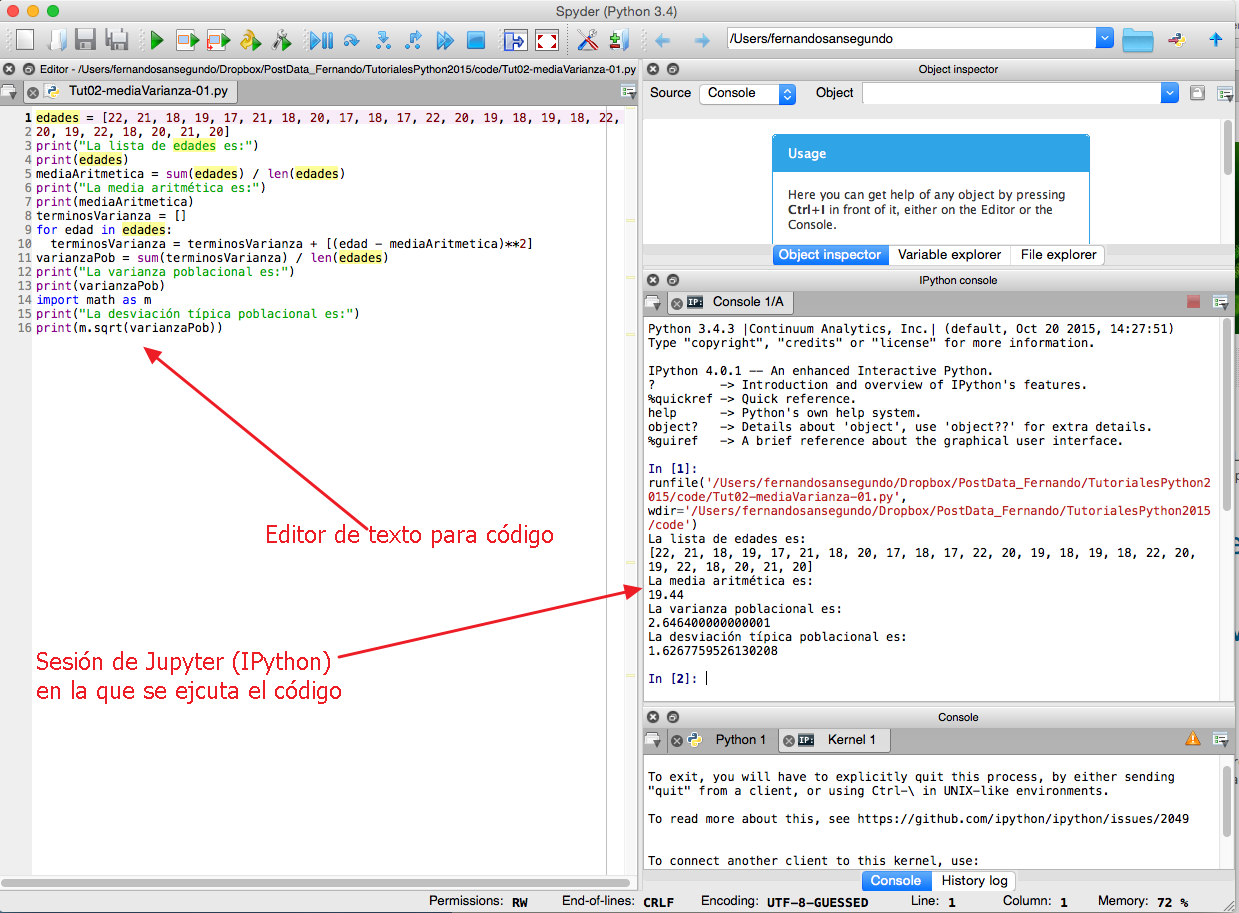
\includegraphics[width=15cm]{../fig/Tut02-py-08-SpyderCapturaPantalla.png}
\end{center}
En estos tutoriales no vamos a entrar en detalles sobre el uso de Spyder o de cualquier otro IDE. Muchos programadores trabajan siempre con la combinación de editor de texto + consola IPython que hemos descrito antes (y un tercer ingrediente que no hemos detallado, la consola de comandos para otras herramientas de desarrollo). Lo que queremos decir con esto es que no hay un entorno de trabajo único para programar en Python. Con el tiempo y la experiencia podrás seleccionar las herramientas que te resulten más cómodas y productivas.

\subsection{Comentarios. }
\label{tut02:subsec:comentarios}

Hemos insistido ya varias veces en que la legibilidad del código es crucial y debe ser una preocupación constante de cualquier programador. Es algo que se debe aprender desde el principio, para incorporarlo a tu conjunto de buenas prácticas científicas.  En el trabajo científico la colaboración entre investigadores y la difusión del conocimiento juegan un papel crucial. Y puesto que la computación es en la actualidad una parte insoslayable de de ese trabajo, es cada vez más común y necesario compartir con otras personas el código que escribimos. A la vez que naturalmente nos convertimos en receptores y usuarios de código escrito por otros.  Con esa idea en mente, la legibilidad del código resulta ser una necesidad imperiosa. Y la elección de nombres adecuados para las variables es sólo el primer paso. Lo que realmente se necesita es una buena {\sf documentación} del código.

Documentar significa, en el contexto de los ficheros de código, añadir a esos ficheros información que no está pensada para dar instrucciones al ordenador, sino que ha sido  pensada para ayudarnos a entender lo que se está haciendo en ese programa. Es decir, esa información no es para la máquina. Es para nosotros mismos, o para otros usuarios (humanos) de ese fichero. A lo largo del curso, en los tutoriales, nosotros te vamos a facilitar una serie de ficheros (los llamaremos {\em ``plantillas''}), que contienen código preparado para llevar a cabo algunos de los métodos que vamos a aprender en cada capítulo del curso. Cuando abras por primera vez uno de esos ficheros, y especialmente al tratarse de métodos con los que, aún, no estás familiarizado, necesitarás sin duda unas ``instrucciones de manejo'', para saber como utilizar el fichero. Esas instrucciones podrían ir en un fichero aparte, claro. Pero la experiencia ha demostrado que esa no es una buena manera de organizar el trabajo. Si el código y la documentación van por separado, es casi inevitable que, al final, tras algunos cambios, ya no se correspondan, y la documentación pase a ser contraproducente.  Afortunadamente, a lo largo del tiempo se han desarrollado una serie de métodos para garantizar una correcta documentación del código, que van desde los más sencillos hasta ideas sofisticadas como el control de versiones y la programación literaria. Aquí vamos a empezar por la manera más sencilla de combinar código y documentación. Más adelante tal vez necesites métodos más sofisticados, pero esos métodos se añadirán a lo que vamos a aprender aquí, sin remplazarlo.

La idea básica es que cuando usamos el símbolo \verb&#& en una línea de código, Python ignora todo el código que aparezca en esa línea a la derecha del símbolo \verb&#&. Vamos a comprobar esto. Hemos ejecutado en la terminal de IPython los siguientes comandos:
\begin{knitrout}
\definecolor{shadecolor}{rgb}{0.969, 0.969, 0.969}\color{fgcolor}\begin{kframe}
\begin{alltt}
\hlstd{In [}\hlnum{1}\hlstd{]}\hlopt{:} \hlstd{a} \hlkwb{=} \hlnum{1}

\hlstd{In [}\hlnum{2}\hlstd{]}\hlopt{:} \hlstd{a} \hlkwb{=} \hlstd{a} \hlopt{+} \hlnum{2}

\hlstd{In [}\hlnum{3}\hlstd{]}\hlopt{:} \hlkwd{print}\hlstd{(a)}
\hlnum{3}
\end{alltt}
\end{kframe}
\end{knitrout}
¿Todo normal, verdad? Ahora, para empezar desde cero, he reiniciado la terminal de IPython. Puedes cerrar Spyder y abrirlo de nuevo, o puedes usar la función mágica \verb#%reset#.
En cualquier caso, ahora ejecutamos el mismo código pero introduciendo el símbolo \verb&#& al principio de la segunda fila:
\begin{knitrout}
\definecolor{shadecolor}{rgb}{0.969, 0.969, 0.969}\color{fgcolor}\begin{kframe}
\begin{alltt}
In [4]: %reset

Once deleted, variables cannot be recovered. \hlkwd{Proceed} (y/[n])? y

In [5]: a = 1

In [6]: \hlcom{# a = a + 2}

In [7]: \hlkwd{print}(a)
1
\end{alltt}
\end{kframe}
\end{knitrout}
Si haces esto verás que desde el mismo momento en que escribes \verb&#& la línea cambia de aspecto. IPython te está indicando visualmente que ese código no se va a ejecutar. Y el resultado confirma que Python ha ignorado esa línea.  Vamos a practicar esto en un ejercicio:

\begin{ejercicio}
\label{tut02:ejercicio18}
\quad
¿Qué va a ocurrir al ejecutar estas tres versiones del código? Trata de adivinarlo antes de hacerlo.
\begin{enumerate}
\item
\begin{knitrout}
\definecolor{shadecolor}{rgb}{0.969, 0.969, 0.969}\color{fgcolor}\begin{kframe}
\begin{alltt}
%reset
a = 1
a = a \hlcom{# + 2}
\hlkwd{print}(a)
\end{alltt}
\end{kframe}
\end{knitrout}
\item
\begin{knitrout}
\definecolor{shadecolor}{rgb}{0.969, 0.969, 0.969}\color{fgcolor}\begin{kframe}
\begin{alltt}
%reset
a = 1
a = a  + \hlcom{# 2}
\hlkwd{print}(a)
\end{alltt}
\end{kframe}
\end{knitrout}
\item
\begin{knitrout}
\definecolor{shadecolor}{rgb}{0.969, 0.969, 0.969}\color{fgcolor}\begin{kframe}
\begin{alltt}
%reset
a = 1
a = a  + 2 \hlcom{# Este caso es interesante.}
\hlkwd{print}(a)
\end{alltt}
\end{kframe}
\end{knitrout}
\end{enumerate}
\quad\\
%Solución en la página \pageref{tut02:ejercicio18:sol}.
\qed
\end{ejercicio}
El último caso de este ejercicio es, en efecto, interesante. Ese ejemplo muestra como podemos utilizar el símbolo \verb&#& para introducir comentarios en medio del código Python. Esas líneas de comentario son extremadamente útiles para explicar lo que está sucediendo en el código, el papel que juegan las variables o para dar al usuario instrucciones precisas sobre el funcionamiento del programa. Imagínate que quieres compartir con alguien el fichero
\paragraph{}\label{fichero:Tut02-mediaVarianza-01}\quad
\begin{knitrout}
\definecolor{shadecolor}{rgb}{0.969, 0.969, 0.969}\color{fgcolor}\begin{kframe}
\begin{alltt}
Tut02-mediaVarianza-01.py
\end{alltt}
\end{kframe}
\end{knitrout}
que hemos escrito antes. Compara la versión original del programa con esta otra en la que hemos usado bastantes comentarios y hemos dejado líneas en blanco:


\begin{knitrout}
\definecolor{shadecolor}{rgb}{0.969, 0.969, 0.969}\color{fgcolor}\begin{kframe}
\begin{alltt}
\hlcom{########################################################}
\hlcom{# www.postdata -statistics.com}
\hlcom{# POSTDATA. Introducción a la Estadística}
\hlcom{# Tutorial 02 (versión Python).}
\hlcom{# Ejemplo de cálculo de media, varianza y desv. típica}
\hlcom{# para una variable cuantitativa, datos no agrupados.}
\hlcom{########################################################}

import math as m

\hlcom{# Esta es la lista de datos sobre la que vamos a trabajar:}
edades = [22, 21, 18, 19, 17, 21, 18, 20, 17, 18, 17, 22, 20, 19, 18, 19, 18, 22, 
20, 19, 22, 18, 20, 21, 20]

\hlcom{# La lista se muestra en pantalla:}
\hlkwd{print}(\hlstr{"La lista de edades es:"})
\hlkwd{print}(edades)

\hlcom{# Media aritmética de la lista:}
mediaAritmetica = \hlkwd{sum}(edades) / \hlkwd{len}(edades)
\hlkwd{print}(\hlstr{"La media aritmética es:"})
\hlkwd{print}(mediaAritmetica)

\hlcom{# Varianza poblacional de la lista}
terminosVarianza = []
for edad in edades:
\hlcom{  # Terminos varianza acumula resultados parciales del numerador de la }
\hlcom{  # varianza en cada iteración del bucle for.}
  terminosVarianza = terminosVarianza + [(edad - mediaAritmetica)**2] 
varianzaPob = \hlkwd{sum}(terminosVarianza) / \hlkwd{len}(edades)
\hlkwd{print}(\hlstr{"La varianza poblacional es:"})
\hlkwd{print}(varianzaPob)

\hlcom{# Desviación típica poblacional.}
\hlkwd{print}(\hlstr{"La desviación típica poblacional es:"})
\hlkwd{print}(\hlkwd{m.sqrt}(varianzaPob))
\end{alltt}
\end{kframe}
\end{knitrout}
Las primeras líneas del programa son un bloque de comentarios que proporciona información sobre el programa, su procedencia, autoría y el objetivo del código. Es bueno incluir ese tipo de información en nuestros programas. A continuación hemos importado el módulo math con el alias {\tt m}. Una de las {\sf recomendaciones de estilo} que forman parte de las buenas prácticas recomendadas al escribir código Python consiste en colocar todas importaciones de módulos al principio del código, para que sean fáciles de loclaizar. Además, como ves, hemos usado líneas en blanco para dividir el programa en bloques lógicos, donde cada bloque de código persigue una finalidad concreta y diferenciada del resto del programa. Esas líneas en blanco no tienen ningún efecto a la hora de ejecutar el programa, pero ayudan a la legibilidad. Y cada bloque comienza con una línea o más de comentarios \verb&#& que describe lo que sucede en ese bloque. En algunos casos se añaden líneas de comentario adicionales dentro del bloque de código, como hemos hecho en el caso del bucle {\tt for} de cálculo de la varianza poblacional, si creemos que eso es necesario para ayudar al lector del programa. El resultado , con la ayuda de colores y tipos de letra adecuados, es un programa del que resulta mucho más fácil entender la estructura y finalidad, un programa más legible. Es importante incorporar esa disciplina a nuestro método de trabajo y pensar siempre que escribimos nuestros programas para que los pueda leer un lector humano. Al principio, especialmente al escribir programas cortos, es posible que pienses que es una pérdida de tiempo introducir tantos comentarios y prestar tanta atención a la documentación del código. Créenos: la forma más segura de perder el tiempo es no hacerlo.

Hemos hablado en el párrafo anterior sobre las recomendaciones de estilo en programas Python. Es un poco prematuro profundizar en esas normas cuando hemos avanzado tan poco todavía, pero para que nos sirva de referencia aquí tienes un enlace a un documento en el que se explicitan algunas de esas recomendaciones de estilo:
\begin{center}
\link{https://www.python.org/dev/peps/pep-0008}{https://www.python.org/dev/peps/pep-0008}
\end{center}

A lo largo del curso iremos comentando otros aspectos relacionados con las buenas prácticas en la documentación del código.

\section{Ficheros {\tt csv} en Python.}
\label{tut02:sec:ficherosCsvPython}

En esta sección vamos a aprender a utilizar ficheros {\tt csv} con Python.  En el Tutorial-01 hemos visto algunos ejemplos de ese tipo de ficheros, y el manejo básico con una hoja de cálculo, como Calc. Como vimos allí, un fichero {\tt csv} típico contiene una tabla de datos, con varias columnas. Esa estructura de tabla se hará imprescindible más adelante. Pero durante una buena parte del curso, nosotros nos vamos a limitar a problemas en los que interviene una única variable. En tal caso, para almacenar los datos de esa variable nos podemos a limitar a considerar un tipo de ficheros {\tt csv} muy básico, como el fichero adjunto:
\begin{center}
\fichero{../datos/Tut02-Edades.csv}{Tut02-Edades.csv}
\end{center}
Guárdalo en la subcarpeta {\tt datos} de tu directorio de trabajo (recuerda la estructura de directorios que hemos creado en el Tutorial-00 para que el código del curso funcione sin problemas). Si abres ese fichero con un editor de texto (como el {\em Bloc de Notas}, en Windows), verás, como muestra esta figura,
\begin{center}
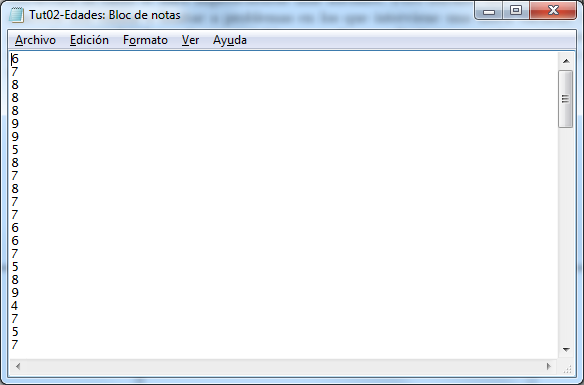
\includegraphics[height=7cm]{../fig/Tut02-06.png}
\end{center}
que el fichero contiene  sólo una columna de datos, que en este ejemplo corresponde a valores de una variable cuantitativa discreta. En la figura sólo se muestra una parte de los datos.
\begin{ejercicio}
\label{tut02:ejercicio19}
\quad\\
¿Cuántos datos hay en ese vector? Usa Calc para averiguarlo, pronto usaremos la función {\tt len} que vimos antes para hacerlo con Python.
%Solución en la página \pageref{tut02:ejercicio19:sol}.
\qed
\end{ejercicio}

\subsubsection*{Leyendo datos de un fichero csv.}
\label{tut02:subsubsec:leyendoDatosFicheroCsv}

Queremos utilizar los datos de ese fichero en Python, y para eso vamos a
\begin{enumerate}
\item leerlos desde el fichero y
\item guardarlos en un vector. El resultado será como si nosotros hubiéramos creado ese vector tecleándo sus elementos directamente.
\end{enumerate}
El código que vamos a utilizar para esto hace uso de la función \verb#read_csv# que debemos importar desde el módulo {\tt pandas}. A lo largo del curso nos vamos a encontrar en varias ocasiones con este módulo que contiene muchas funciones orientadas a la Estadística  y el Análisis de Datos. Los comandos necesarios para las operaciones que hemos descrito aparecen aquí debajo. Los comentaremos uno a uno a continuación:
\begin{knitrout}
\definecolor{shadecolor}{rgb}{0.969, 0.969, 0.969}\color{fgcolor}\begin{kframe}
\begin{alltt}
%cd ~/Desktop/PostData/
import pandas as pd
listaEdades = \hlkwd{pd.read_csv}(\hlstr{"./datos/Tut02-Edades.csv"}, names=[\hlstr{"edades"}])
listaEdades = listaEdades[\hlstr{"edades"}]\hlkwd{.tolist}()
\hlkwd{print}(listaEdades)
\end{alltt}
\end{kframe}
\end{knitrout}
Al ejecutar este código en IPython esto es lo que sucede:
\begin{knitrout}
\definecolor{shadecolor}{rgb}{0.969, 0.969, 0.969}\color{fgcolor}\begin{kframe}
\begin{alltt}
In [1]: %cd ~/Desktop/PostData/
/Users/fernando/Desktop/PostData

In [2]: import pandas as pd

In [3]: listaEdades = \hlkwd{pd.read_csv}(\hlstr{"./datos/Tut02-Edades.csv"}, names=[\hlstr{"v"}])

In [4]: listaEdades = listaEdades[\hlstr{"v"}]\hlkwd{.tolist}()

In [5]: \hlkwd{print}(listaEdades)
[6, 7, 8, 8, 8, 9, 9, 5, 8, 7, 8, 7, 7, 6, 6, 7, 5, 8, 9, 4, 7, 5, 7, 7, 5, 9, 4,
7, 7, 7, 8, 5, 8, 9, 7, 4, 6, 6, 6, 9, 8, 6, 7, 6, 7, 6, 6, 8, 6, 5, 5, 6, 6, 8,
5, 8, 5, 9, 7, 6, 9, 5, 7, 8, 8, 7, 10, 7, 8, 7, 5, 6, 8, 8, 7, 3, 5, 6, 7, 5, 7,
7, 5, 8, 4, 8, 8, 8, 6, 7, 6, 6, 8, 5, 6, 5, 8, 6, 9, 7]
\end{alltt}
\end{kframe}
\end{knitrout}
Vamos a ver paso a paso cómo se  ha leído el contenido de ese fichero de datos y se ha convertido en la lista {\tt listaEdades}. No es necesario que en este momento entiendas todos los detalles que vamos a presentar (y la misma observación sirve para el resto de métodos de lectura/escritura que vamos a ver en esta sección). Basta con una comprensión somera del método para que puedas aplicarlo a la lectura de otros ficheros de datos similares. Más adelante, cuando hayas ganado confianza con Python, podrás volver aquí y tratar de entender en detalle cómo funciona la lectura de datos.
\begin{itemize}

\item La primera línea usa la {\tt función mágica} {\tt cd} que ya conocemos para decirle a Python cuál es nuestro directorio de trabajo. En mi caso es la carpeta {\em PostData} dentro del {\em Escritorio (Desktop)}, pero tú tendrás que ajustarla a tu situación particular.

\item La segunda línea simplemente importa el módulo {\tt pandas} con el alias {\tt pd}, que es el que la mayoría de programadores de Python usan habitualmente para este módulo.

\item La tercera línea es la más iportante: aquí es donde usamos la función \verb#read_csv# para leer los datos del fichero. Pero {\tt pandas} es una librería sofisticada, diseñada para problemas complejos. Así que la función \verb#read_csv# es capaz de leer ficheros de datos bastante más complejos que el que estamos usando como ejemplo. En particular, el resultado de \verb#read_csv# {\bf no es una lista}, sino un objeto propio de {\tt pandas} llamado {\tt DataFrame} y pensado para almacenar una tabla con varias columnas. En nuestro caso se trata de una tabla con una única columna, pero aún así {\tt pandas} sigue pensando en este objeto como una tabla. En la cuarta línea lo convertiremos en una lista. Pero para eso, por razones técnicas, tenemos que darle un nombre a la  columna (única) que contiene los datos. Por eso aparece el argumento opcional \verb#names=["edades"]# en la función \verb#read_csv#.

\item En la cuarta línea de código llevamos a cabo la conversión de la columna del {\tt DataFrame} que hemos llamado {\tt edades} en una lista. Para ello seleccionamos esa columna mediante \verb#listaEdades["edades"]#. Fíjate en que esa forma de seleccionar con corchetes es parecida a la selección de elementos de listas, aunque aquí seleccionamos por nombre y no por posición. Después de seleccionar la columna invocamos el método {\tt tolist} que convierte esa columna en una lista.
\end{itemize}
En el siguiente ejercicio vas a tener ocasión de practicar la lectura de este tipo de ficheros {\tt csv}.
\begin{ejercicio}
\label{tut02:ejercicio20}
\quad\\

Guarda el fichero de datos adjunto:
\begin{center}
\fichero{../datos/Tut02-ejercicioLecturaCsv.csv}{Tut02-ejercicioLecturaCsv.csv}
\end{center}
en tu carpeta datos. Ábrelo primero con un editor de texto para hacer una exploración preliminar del fichero. {\bf ¡Acostúmbrate a hacer siempre esto!} Después usa el método que hemos visto para leer los datos del fichero con Python y calcula la media aritmética de esos datos.
%Solución en la página \pageref{tut02:ejercicio20:sol}.
\qed
\end{ejercicio}
Para cerrar este apartado, es conveniente haber visto el formato del mensaje de error que se produce cuando el fichero que tratamos de leer desde Python no existe, o no está en el directorio de trabajo.
\begin{ejercicio}
\label{tut02:ejercicio21}
\quad\\
Prueba a ejecutar:
\begin{knitrout}
\definecolor{shadecolor}{rgb}{0.969, 0.969, 0.969}\color{fgcolor}\begin{kframe}
\begin{alltt}
\hlkwd{pd.read_csv}(\hlstr{"./datos/EsteFicheroNoExiste.csv"}, names=[\hlstr{"v"}])
\end{alltt}
\end{kframe}
\end{knitrout}
y fíjate en el mensaje de error.
%Solución en la página \pageref{tut02:ejercicio21:sol}.
\qed
\end{ejercicio}

\subsubsection*{Otro formato del fichero de datos.}
\label{tut02:subsubsec:otroFormatoFicheroDatos}

% En este apartado vamos a usar los datos del fichero adjunto:
% \begin{center}
% \fichero{../datos/Tut02-Edades2.csv}{Tut02-Edades2.csv}
% \end{center}

Los ficheros {\tt  csv} que contienen un único vector (en lugar de una {\em tabla} de datos), pueden adoptar formatos distintos del que acabamos de ver. Por ejemplo, el fichero adjunto
\begin{center}
\fichero{../datos/Tut02-Edades2.csv}{Tut02-Edades2.csv}
\end{center}
contiene los mismos datos que {\tt Tut02-Edades.csv}, pero ahora los datos del vector están todos en una fila, y separados por comas. Guárdalo, como antes, en la subcarpeta {\tt datos} de tu directorio de trabajo. El aspecto del fichero, visto a través de un editor de texto, es este (sólo son visibles una parte de los datos):
    \begin{center}
    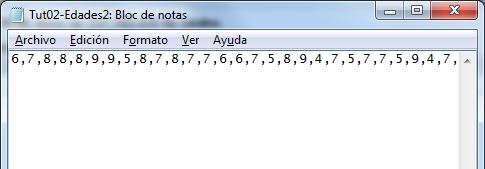
\includegraphics[width=12cm]{../fig/Tut02-07a.png}
    \end{center}
Desde luego, no nos podemos plantear transformar a mano este vector en uno como el del apartado anterior. Podríamos buscar soluciones pasando por la hoja de cálculo (por ejemplo: lo leeríamos en una fila de la hoja, y luego habría que usar el {\tt Pegado especial} para trasponerlo -es decir, girarlo- para finalmente volver a guardarlo). Afortunadamente, hay una solución, sin salir de Python, bastante menos embrollada. Tenemos que usar un argumento opcional de la función \verb#read_csv#, concretamente el argumento {\tt lineterminator} que como su nombre indica sirve para indicarle a {\tt pandas} cuál es el carácter que usamos para separar en líneas nuestro fichero. En la terminal de IPython usamos esta variante del método para leer el fichero (se asume que ya hemos importado {\tt pandas} y que has fijado el directorio de trabajo con \verb#cd#):
{\small
\begin{knitrout}
\definecolor{shadecolor}{rgb}{0.969, 0.969, 0.969}\color{fgcolor}\begin{kframe}
\begin{alltt}
In [12]: listaEdades2 = \hlkwd{pd.read_csv}(\hlstr{"./datos/Tut02-Edades2.csv"}, names=[\hlstr{"edades"}], lineterminator=\hlstr{","})

In [13]: listaEdades2 = listaEdades2[\hlstr{"edades"}]\hlkwd{.tolist}()

In [14]: \hlkwd{print}(listaEdades2)
[6, 7, 8, 8, 8, 9, 9, 5, 8, 7, 8, 7, 7, 6, 6, 7, 5, 8, 9, 4, 7, 5, 7, 7, 5, 9, 4, 7, 7, 7,
8, 5, 8, 9, 7, 4, 6, 6, 6, 9, 8, 6, 7, 6, 7, 6, 6, 8, 6, 5, 5, 6, 6, 8, 5, 8, 5, 9, 7, 6,
9, 5, 7, 8, 8, 7, 10, 7, 8, 7, 5, 6, 8, 8, 7, 3, 5, 6, 7, 5, 7, 7, 5, 8, 4, 8, 8, 8, 6, 7,
6, 6, 8, 5, 6, 5, 8, 6, 9, 7]
\end{alltt}
\end{kframe}
\end{knitrout}
}
Como en el apartado anterior, el resultado es una lista de Python que contiene los datos del fichero {\tt csv}.

\subsubsection*{Escribiendo datos a un fichero csv.}
\label{Tut02:subsubsec:escribiendoDatosFicheroCsv}
Para completar nuestra primera visita al manejo de ficheros {\tt csv} desde Python vamos a recorrer el camino inverso. Porque muchas veces, después de hacer operaciones en Python, obtendremos como resultados listas de datos interesantes (y, más adelante en el curso, otro tipo de objetos, como tablas). Lo natural, entonces, es aprender a guardar esos datos en un fichero de tipo csv, como el fichero con el que empezamos. De esa forma, por ejemplo, puedes compartir tus resultados con otras personas, incluso aunque no utilicen Python.

Vamos a practicar esto escribiendo a un fichero csv la siguiente lista de datos:
% Para ello, si antes usábamos la función \verb#read_csv# de {\tt pandas}, ahora vamos a usar la función  de R.

\begin{knitrout}
\definecolor{shadecolor}{rgb}{0.969, 0.969, 0.969}\color{fgcolor}\begin{kframe}
\begin{alltt}
edades3 = [29, 28, 36, 41, 41, 33, 28, 32, 35, 36, 36, 33, 40, 41, 28, 30, 27, 33, 38, 36]
\end{alltt}
\end{kframe}
\end{knitrout}
Para hacerlo seguimos un camino inverso al de los apartados anteriores. Primero usamos una función de {\tt pandas} llamada también {\tt DataFrame} que convertirá nuestra lista en un objeto de ese tipo {\tt DataFrame}, que como ya hemos dicho es la estructura de datos básica de {\tt pandas} para representar datos. Recuerda que se supone que hemos importado {\tt pandas} con el alias {\tt pd}:
\begin{knitrout}
\definecolor{shadecolor}{rgb}{0.969, 0.969, 0.969}\color{fgcolor}\begin{kframe}
\begin{alltt}
\hlstd{edades3pd} \hlkwb{=} \hlkwd{pd.DataFrame}\hlstd{(edades3)}
\end{alltt}
\end{kframe}
\end{knitrout}
Hemos añadido {\tt pd} al final del nombre simplemente como recordatorio de que el resultado es un objeto propio de {\tt pandas}. Ahora usamos el método \verb#to_csv# de ese objeto. Recuerda la sintaxis de objetos y métodos que vimos en el apartado \ref{tut02:subsubsec:ordenacionLista} (pág. \pageref{tut02:subsubsec:ordenacionLista}):

\begin{knitrout}
\definecolor{shadecolor}{rgb}{0.969, 0.969, 0.969}\color{fgcolor}\begin{kframe}
\begin{alltt}
\hlkwd{edades3pd.to_csv}\hlstd{(}\hlstr{"./datos/Tut02py-Edades-3.csv"}\hlstd{,} \hlkwc{header}\hlstd{=False,} \hlkwc{index}\hlstd{=False)}
\end{alltt}
\end{kframe}
\end{knitrout}
Los argumentos {\tt header=False} e {\tt index=False} sirven respectivamente para evitar que {\tt pandas} añada al fichero csv una línea de encabezamiento y que numere cada una de las líneas de datos.
\begin{ejercicio}
\label{tut02:ejercicio22}
\quad\\
Usa un editor de texto para explorar el fichero {\tt csv} resultante. Comprueba lo que sucede si eliminas uno o ambos argumentos opcionales del método  \verb#to_csv#
%Solución en la página \pageref{tut02:ejercicio22:sol}.
\qed
\end{ejercicio}
Con esto concluye nuestra breve visita al al manejo de ficheros {\tt csv} desde Python. A lo largo del curso aprenderemos más sobre este ingrediente fundamental para poder comunicar nuestras sesiones de trabajo en Python con el mundo exterior.

\section{Estadística descriptiva de una variable cuantitativa discreta con datos no agrupados.}
\label{tut02:sec:estadisticaDescriptiva}

Con el trabajo de las secciones previas estamos listos para abordar el objetivo principal de este tutorial: dada una muestra
\[
x_1, x_2, \ldots, x_n
\]
de una variable cuantitativa vamos a describir esa muestra calculando sus medidas centrales o de posición(media, mediana), las medidas de dispersión (varianza, desviación típica) y además las representaciones gráficas que nos ayudan a hacernos una mejor idea de las propiedades de esa muestra.
El punto de partida será un fichero {\tt csv} que contiene los datos de la muestra. Supondremos que en ese fichero los datos están en columna, de manera que hay un único dato en cada fila del fichero. Si no es así, ya hemos visto cómo adaptar el código a otras situaciones frecuentes. En esta sección vamos a usar como ejemplo el fichero adjunto:
\begin{center}
  \fichero{../datos/Tut02-var3.csv}{Tut02-var3.csv}
\end{center}

\begin{ejercicio}
\label{tut02:ejercicio23}
\quad\\
Antes de seguir adelante guarda el fichero {\tt Tut02-var3.csv} en la carpeta {\tt datos} del {\em Directorio de trabajo} y usa un editor de texto para explorar ese fichero {\tt csv}.
%Solución en la página \pageref{tut02:ejercicio23:sol}.
\qed
\end{ejercicio}

Para analizar estos datos vamos a utilizar un fichero de código Python, el primero de nuestros {\em ``ficheros plantilla''} de estos tutoriales, que calcule de forma automática todas esas medidas descriptivas. Vamos a ir describiendo el contenido de ese fichero, que aparece aquí adjunto:
\begin{center}
\fichero{./code/Tut02-estadisticaDescriptiva.py}{Tut02-estadisticaDescriptiva.py}
\end{center}
Abre el fichero en un editor de texto para ir recorriendo el código a medida que lo comentamos. Lo mejor es que sea un editor con reconocimiento de sintaxis.

Antes de seguir queremos aclarar un detalle técnico. Cuando abras el fichero verás que incluye unas cuantas líneas de comentario que empiezan con \verb&## ----&. La razón por la que hacemos esto tiene que ver con la herramienta de documentación que usamos para escribir estos tutoriales, y no es una característica de Python. Recuerda que lo que caracteriza a un comentario en Python es la presencia del símbolo \verb&#&.



\subsubsection*{Cabecera del fichero.}
\label{tut02:subsubsec:cabeceraFichero}

Lo primero que verás en el fichero es un bloque inicial de comentarios que sirven para identificar y describir el programa. A continuación aparecen unas instrucciones básicas de uso, que nos recuerdan la necesidad de tener en cuenta cuál es el directorio de trabajo y de la ubicación de los ficheros necesarios respecto de ese directorio.
\begin{knitrout}
\definecolor{shadecolor}{rgb}{0.969, 0.969, 0.969}\color{fgcolor}\begin{kframe}
\begin{alltt}
\hlcom{########################################################}
\hlcom{# www.postdata-statistics.com}
\hlcom{# POSTDATA. Introducción a la Estadística}
\hlcom{# Tutorial 02.  }
\hlcom{# Plantilla de comandos Python para Estadística Descriptiva}
\hlcom{# Una variable cuantitativa discreta, datos no agrupados.}
\hlcom{########################################################}


\hlcom{# ATENCION: para que este fichero funcione es NECESARIO: }
\hlcom{# (1) tener en cuenta la estructura de directorios como se explica en el tutorial. }
\hlcom{# (2) introducir el nombre del fichero de datos como argumento de read_csv.}
\end{alltt}
\end{kframe}
\end{knitrout}
Para que el fichero funcione correctamente es necesario respetar la estructura de directorios que hemos creado en el Tutorial-00. Recordemos:
\begin{itemize}
\item En tu ordenador existe una carpeta a la que nos referiremos siempre como {\em Directorio de trabajo} del curso.
\item El {\em Directorio de trabajo} contiene una subcarpeta llamada {\em datos}, en la que están situados los ficheros {\tt csv} que vamos a utilizar.
\item El {\em Directorio de trabajo} contiene además otra subcarpeta lllamada {\tt code} en la que están situados los ficheros de código Python para ejecutar con IPython (con extensión {\tt ipy}).
\end{itemize}
Más abajo veremos como ejecutar el fichero en la terminal de IPython. Pero para que todo funcione correctamente es esencial respetar esta estructura de directorios. Daremos más detalles sobre la segunda de esas instrucciones, al llegar a la línea pertinente del código.

\subsubsection*{Importando módulos.}
\label{tut02:subsubsec:importandoModulos}

El siguiente bloque contiene las líneas de código en las que se importan los módulos que vamos a utilizar.
\begin{knitrout}
\definecolor{shadecolor}{rgb}{0.969, 0.969, 0.969}\color{fgcolor}\begin{kframe}
\begin{alltt}
import pandas as pd 
import numpy as np 
import matplotlib.pyplot as plt 
import collections as cl 
\end{alltt}
\end{kframe}
\end{knitrout}
Las recomendaciones de estilo de Python especifican que todos los módulos deben importarse al comienzo del programa y que cada módulo debe importarse en una línea propia. Hemos aprovechado esa circunstancia para colocar, junto a cada módulo, un comentario que enumera las funciones de ese módulo que vamos a usar. Fíjate además en que hemos usado alias para los nombres de todos los módulos (de hecho algunos de estos alias son un estándar {\em de facto} entre los programadores de Python). Ya conoces el módulo {\tt pandas}. Vamos a usar también el módulo {\tt numpy} que contiene muchos objetos y funciones para el Cálculo Numérico. Más adelante en el curso tendremos ocasión de discutir sobre los aspectos numérico y simbólico de las Matemáticas. Por el momento nos conformamos con señalar que {\tt numpy} es uno de los pilares básicos del cálculo científico con Python. Por su parte {\tt matplotlib} es un módulo especializado en gráficas matemáticas, que vamos a usar para dibujar diagramas de barras, de cajas, histogramas, etc. Finalmente, el módulo {\tt collections} aparecerá varias veces en estos tutoriales, pero aquí concretamente lo usaremos para fabricar fácilmente las tablas de frecuencias de nuestros datos.


\subsubsection*{Preliminares.}
\label{tut02:subsubsec:preliminares}

A continuación se incluye un bloque que puede servir para definir algunas variables que se usarán a lo largo del resto del programa.
\begin{knitrout}
\definecolor{shadecolor}{rgb}{0.969, 0.969, 0.969}\color{fgcolor}\begin{kframe}
\begin{alltt}
\hlstd{linea} \hlkwb{=} \hlstr{"_"} \hlopt{*} \hlnum{75}

\hlkwd{print}\hlstd{(linea)}
\hlkwd{print}\hlstd{(linea)}
\hlkwd{print}\hlstd{(}\hlstr{"www.postdata-statistics.com"}\hlstd{)}
\hlkwd{print}\hlstd{(}\hlstr{"Curso de introducción a la Estadística. Tutorial02 (versión Python)."}\hlstd{)}
\hlkwd{print}\hlstd{(}\hlstr{"Estadística descriptiva. Una variable cuantitativa discreta,\textbackslash{}n datos no agrupados."}\hlstd{)}
\hlkwd{print}\hlstd{(linea)}
\hlkwd{print}\hlstd{(linea)}
\end{alltt}
\end{kframe}
\end{knitrout}

La variable definida mediante \verb&linea = "_"*75& se usa simplemente para dibujar una línea horizontal, y separar así la salida del programa en bloques temáticos. Cada vez que queramos imprimir esa línea separadora usaremos el comando {\tt print(linea)}.

Además, usando {\tt print}, se incluyen en este bloque algunos mensajes que se mostrarán al ejecutar este programa. Siempre es necesario proporcionar al menos esa información básica al usuario.

\subsubsection*{Lectura del fichero de datos. Ejecución del código.}
\label{tut02:subsubsec:lecturaDatos}

A continuación tenemos el bloque en el que se lee el fichero {\tt csv} que contiene los datos:
\begin{knitrout}
\definecolor{shadecolor}{rgb}{0.969, 0.969, 0.969}\color{fgcolor}\begin{kframe}
\begin{alltt}
\hlcom{# Lectura de los datos:}
\hlcom{# INTRODUCIR EL NOMBRE DEL FICHERO DE DATOS EN LA SIGUIENTE LINEA:}
\hlcom{# EL FICHERO DEBE RESIDIR EN LA CARPETA DATOS DEL DIR. DE TRABAJO}
nombreFichero = \hlstr{"Tut02-var3.csv"}
datos = \hlkwd{pd.read_csv}(\hlstr{"../../datos/"} + nombreFichero, names=[\hlstr{"v"}])
datos = datos[\hlstr{"v"}]\hlkwd{.tolist}()

\hlkwd{print}(\hlstr{"El fichero de datos es:"})
\hlkwd{print}(nombreFichero)

n = \hlkwd{len}(datos)
\hlkwd{print}(\hlstr{"El número de datos leídos es:"})
\hlkwd{print}(n)

\hlkwd{print}(\hlstr{"Los primeros 10 datos son:"})
\hlkwd{print}(datos[:10])
\hlkwd{print}(\hlstr{"Los últimos 10 datos son:"})
\hlkwd{print}(datos[-10:])

\hlkwd{print}(linea)
\end{alltt}
\end{kframe}
\end{knitrout}
Como ves, para leer los datos se usa la función \verb&read_csv& de {\tt pandas} que ya conocemos. Para un uso correcto del código {\bf es esencial} introducir el nombre del fichero {\tt csv} en la línea adecuada. Después se usa la concatenación (suma) de cadenas de caracteres para obtener como argumento de la función \verb&read_csv& el nombre completo del fichero (incluida la carpeta en la que se encuentra) .

Una vez que hemos introducido el nombre del fichero de datos, nos aseguramos de grabar el fichero de código con esa modificación y ya podemos ejecutarlo. Ve a la terminal de IPython y usa las funciones mágicas \verb&%cd&
y \verb&%run&
como hemos visto para ejecutar este fichero de código. Es decir:
\begin{knitrout}
\definecolor{shadecolor}{rgb}{0.969, 0.969, 0.969}\color{fgcolor}\begin{kframe}
\begin{alltt}
In [1]: %cd ~/Desktop/PostData
/Users/fernando/Desktop/PostData

In [2]: %run ./code/Tut02-estadisticaDescriptiva.py
\end{alltt}
\end{kframe}
\end{knitrout}
Si todo va bien cuando ejecutes la función \verb&%run&
verás aparecer los resultados que produce el programa. En los párrafos que siguen vamos a ir ostrando esos resultados inmediatamente detrás del correspondiente fragmento de código. Por ejemplo, lo primero que hace el código, para comprobar que la lectura de datos ha sido correcta, es mostrar cuántos son los datos leídos (el número se alamcena en la variable {\tt n}). Además se muestran los primeros 10 y los últimos 10 valores de la lista de datos. En IPython eso se traduce en:
\begin{knitrout}
\definecolor{shadecolor}{rgb}{0.969, 0.969, 0.969}\color{fgcolor}\begin{kframe}
\begin{alltt}
El número de datos leídos es:
1300
Los primeros 10 valores son:
[4, 8, 4, 4, 5, 5, 3, 6, 6, 2]
Los últimos 10 valores son:
[4, 10, 6, 4, 3, 9, 6, 7, 3, 7]
\end{alltt}
\end{kframe}
\end{knitrout}

\subsubsection*{Recorrido de los datos.}
\label{tut02:subsubsec:recorridoDatos}

A continuación vamos a determinar el máximo y mínimo de los datos, que conjuntamente determinan lo que hemos llamado el recorrido.

\begin{knitrout}
\definecolor{shadecolor}{rgb}{0.969, 0.969, 0.969}\color{fgcolor}\begin{kframe}
\begin{alltt}
\hlcom{## Recorrido de una lista de números.  }

\hlkwd{print}\hlstd{(}\hlstr{"El mínimo y máximo de los datos determinan el recorrido:"}\hlstd{)}
\hlkwd{print}\hlstd{(}\hlstr{"Mínimo:"}\hlstd{)}
\hlkwd{print}\hlstd{(}\hlkwd{min}\hlstd{(datos))}

\hlkwd{print}\hlstd{(}\hlstr{"Máximo:"}\hlstd{)}
\hlkwd{print}\hlstd{(}\hlkwd{max}\hlstd{(datos))}

\hlkwd{print}\hlstd{(}\hlstr{"La anchura del recorrido (max - min) es:"}\hlstd{)}

\hlkwd{print}\hlstd{(}\hlkwd{max}\hlstd{(datos)} \hlopt{-} \hlkwd{min}\hlstd{(datos))}

\hlkwd{print}\hlstd{(linea)}
\end{alltt}
\end{kframe}
\end{knitrout}

El resultado es:
\begin{knitrout}
\definecolor{shadecolor}{rgb}{0.969, 0.969, 0.969}\color{fgcolor}\begin{kframe}
\begin{alltt}
El mínimo y máximo de los datos determinan el recorrido:
Mínimo:
0
Máximo:
16
La anchura del \hlkwd{recorrido} (max - min) es:
16
\end{alltt}
\end{kframe}
\end{knitrout}

\subsubsection*{Tablas de frecuencia. Tuplas en Python.}
\label{tut02:subsubsec:tablasFrecuenciaTuplas}

Nuestro siguiente objetivo es obtener las tablas de frecuencia de los datos. Primero vamos a construir los valores que deben aparecer en ellas, y después usaremos {\tt print} con formato para mostrar esa información de una manera más cómoda.

Empezamos con la tabla de frecuencias absolutas. Para fabricarla vamos a crear un objeto  de tipo {\tt Counter}, procedente del módulo {\tt collections} (importado con el alias {\tt cl}). El código es este, que comentaremos a continuación:

\begin{knitrout}
\definecolor{shadecolor}{rgb}{0.969, 0.969, 0.969}\color{fgcolor}\begin{kframe}
\begin{alltt}
\hlstd{datos_counter} \hlkwb{=} \hlkwd{cl.Counter}\hlstd{(datos)}
\hlstd{tablaFreqAbs} \hlkwb{=} \hlkwd{datos_counter.most_common}\hlstd{()}
\hlkwd{tablaFreqAbs.sort}\hlstd{()}
\end{alltt}
\end{kframe}
\end{knitrout}

En la primera línea creamos el objeto de tipo {\tt Counter} a partir de la lista {\tt datos}. Estos objetos sirven en Python para obtener tablas de frecuencia, pero también para manipularlas. Para hacer esas operaciones el objeto {\tt Counter} disponde de una serie de métodos. Aquí vamos a usar el método \verb&most_common&, que devuelve como resultado una representación de la tabla de frecuencias como lista de pares. El resultado se almacena en la variable {\tt tablaFreqAbs}. Aunque nuestro código no lo hace, vamos a ver el resultado  después de ejecutar el método \verb&most_common& en la terminal de IPython:

\begin{knitrout}
\definecolor{shadecolor}{rgb}{0.969, 0.969, 0.969}\color{fgcolor}\begin{kframe}
\begin{alltt}
In [25]: tablaFreqAbs = \hlkwd{datos_counter.most_common}()

In [26]: \hlkwd{print}(tablaFreqAbs)
[(5, 246), (4, 244), (3, 188), (6, 186), (7, 131), (2, 100), (8, 87), (9, 43),
(10, 28), (1, 25), (0, 9), (11, 6), (12, 2), (13, 2), (14, 2), (16, 1)]
\end{alltt}
\end{kframe}
\end{knitrout}
El resultado es una tabla de frecuencias, en forma de lista de pares: cada par contiene como primer elemento uno de los números de la lista {\tt datos} y como segundo elemento la frecuencia absoluta de ese número. Pero hay un problema: los pares aparecen desordenados. Y para una tabla de frecuencia lo natural es ordenar los pares usando los valores de {\tt datos}. Por eso hemos aplicado el método {\tt sort} de ordenación {\em in situ}, que da como resultado:
\begin{knitrout}
\definecolor{shadecolor}{rgb}{0.969, 0.969, 0.969}\color{fgcolor}\begin{kframe}
\begin{alltt}
In [28]: \hlkwd{tablaFreqAbs.sort}()

In [29]: \hlkwd{print}(tablaFreqAbs)
[(0, 9), (1, 25), (2, 100), (3, 188), (4, 244), (5, 246), (6, 186), (7, 131),
(8, 87), (9, 43), (10, 28), (11, 6), (12, 2), (13, 2), (14, 2), (16, 1)]
\end{alltt}
\end{kframe}
\end{knitrout}
Y ahora esta  lista sí muestra de forma conveniente la tabla de frecuencias. Más abajo en el código usaremos este resultado para imprimir conjuntamente todas las tablas de frecuencia. Pero no podemos seguir adelante sin comentar algo en lo que tal vez ya hayas reparado. Hemos visto que {\tt tablaFreqAbs} es una lista de {\em pares}. ¿Qué clase de objeto Python son esos pares? Veámoslo. El primero de esos pares se obtiene así, como es de esperar:
\begin{knitrout}
\definecolor{shadecolor}{rgb}{0.969, 0.969, 0.969}\color{fgcolor}\begin{kframe}
\begin{alltt}
In [30]: tablaFreqAbs[0]
Out[30]: (0, 9)
\end{alltt}
\end{kframe}
\end{knitrout}
Y para saber de que tipo es usamos {\tt type}:
\begin{knitrout}
\definecolor{shadecolor}{rgb}{0.969, 0.969, 0.969}\color{fgcolor}\begin{kframe}
\begin{alltt}
\hlstd{In [}\hlnum{31}\hlstd{]}\hlopt{:} \hlkwd{type}\hlstd{(tablaFreqAbs[}\hlnum{0}\hlstd{])}
\hlstd{Out[}\hlnum{31}\hlstd{]}\hlopt{:} \hlstd{tuple}
\end{alltt}
\end{kframe}
\end{knitrout}
Python nos informa de que es un objeto de tipo {\tt tuple}. En español se suele usar {\sf tupla}. La palabra tupla es una generalización de las parejas, tríos, etc., de manera que una tupla es una colección de una cantidad cualquiera de elementos, rodeados por paréntesis. Las tuplas son otra estructura de datos de Python, como las listas y las encontraremos a menudo en estos tutoriales. De momento nos conformamos con saber que existen\footnote{Básicamente, existen por razones técnicas, para hacer el código Python más rápido y eficiente. Todo lo que Python hace usando tuplas se podría hacer con listas, pero el código consumiría más recursos de tiempo y memoria.}, que es muy fácil crearlas y que se accede a sus elementos de forma análoga a lo que se hace con las listas. Un ejemplo sencillo:
\begin{knitrout}
\definecolor{shadecolor}{rgb}{0.969, 0.969, 0.969}\color{fgcolor}\begin{kframe}
\begin{alltt}
In [1]: unaTupla = (1, 2, 6.4, \hlstr{"Hola"})

In [2]: unaTupla[2:4]
Out[2]: (6.4, \hlstr{'Hola'})
\end{alltt}
\end{kframe}
\end{knitrout}
En las operaciones que sigue nos resultará conveniente disponer de dos listas que contengan por separado los elementos que componen las parejas de {\tt tablaFreqAbs}. Para conseguirlo usamos comprensión de listas dos veces:
\begin{knitrout}
\definecolor{shadecolor}{rgb}{0.969, 0.969, 0.969}\color{fgcolor}\begin{kframe}
\begin{alltt}
valoresUnicos = [ item[0] for item in tablaFreqAbs]
freqAbs = [ item[1] for item in tablaFreqAbs]
\end{alltt}
\end{kframe}
\end{knitrout}
El resultado son estas dos listas que mostramos en la terminal de IPython (el programa no las muestra por separado). Aprovecharemos para comprobar que la suma de las frecuencias absolutas es la esperada:
\begin{knitrout}
\definecolor{shadecolor}{rgb}{0.969, 0.969, 0.969}\color{fgcolor}\begin{kframe}
\begin{alltt}
In [32]: valoresUnicos
Out[32]: [0, 1, 2, 3, 4, 5, 6, 7, 8, 9, 10, 11, 12, 13, 14, 16]

In [33]: freqAbs
Out[33]: [9, 25, 100, 188, 244, 246, 186, 131, 87, 43, 28, 6, 2, 2, 2, 1]

In [34]: \hlkwd{sum}(freqAbs)
Out[34]: 1300
\end{alltt}
\end{kframe}
\end{knitrout}
A partir de la lista de frecuencias absolutas es fácil obtener la de frecuencias relativas. Basta con dividir cada frecuencia absoluta por la variable {\tt n}, que almacena el número total de observaciones. Vamos a fabricar esas frecuencias relativas mediante una comprensión de lista:

\begin{knitrout}
\definecolor{shadecolor}{rgb}{0.969, 0.969, 0.969}\color{fgcolor}\begin{kframe}
\begin{alltt}
freqRel = [ item/n for item in freqAbs]
\end{alltt}
\end{kframe}
\end{knitrout}
Como ya hemos anunciado, más abajo usaremos {\tt print} para mostrar todas las frecuencias (absolutas, relativas, etc.) en una misma tabla y con el formato adecuado. Pero podemos mostrar el valor de {\tt freqRel} en la terminal de IPython:

\begin{knitrout}
\definecolor{shadecolor}{rgb}{0.969, 0.969, 0.969}\color{fgcolor}\begin{kframe}
\begin{alltt}
In [35]: \hlkwd{print}(freqRel)
[0.006923076923076923, 0.019230769230769232, 0.07692307692307693,
0.14461538461538462, 0.18769230769230769, 0.18923076923076923,
0.14307692307692307, 0.10076923076923076, 0.06692307692307692,
0.03307692307692308, 0.021538461538461538, 0.004615384615384616,
0.0015384615384615385, 0.0015384615384615385, 0.0015384615384615385,
0.0007692307692307692]
\end{alltt}
\end{kframe}
\end{knitrout}
Cuando usemos {\tt print} para mostrar estos valores los redondearemos a una cantidad adecuada de cifras significativas. De momento podemos usar la terminal de IPython para comprobar que la suma de las frecuencias relativas es $1$, dentro de la precisión que permite el redondeo cuando se trabaja con valores en coma flotante:
\begin{knitrout}
\definecolor{shadecolor}{rgb}{0.969, 0.969, 0.969}\color{fgcolor}\begin{kframe}
\begin{alltt}
\hlstd{In [}\hlnum{36}\hlstd{]}\hlopt{:} \hlkwd{sum}\hlstd{(freqRel)}
\hlstd{Out[}\hlnum{36}\hlstd{]}\hlopt{:} \hlnum{0.9999999999999997}
\end{alltt}
\end{kframe}
\end{knitrout}
Nuestro siguiente objetivo es obtener la tabla de frecuencias acumuladas. Aquí vamos a recurrir por primera vez al módulo {\tt numPy}. Concretamente usaremos la función {\tt cumsum} de ese módulo (el nombre proviene del inglés {\em cumulative sum}, suma acumulada). Pero el resultado de {\tt cumsum} es un objeto de un tipo que aún no hemos visto, el tipo {\tt ndarray} de {\tt numpy}. Por eso usamos el método {\tt tolist} para convertirlo en una lista.
\begin{knitrout}
\definecolor{shadecolor}{rgb}{0.969, 0.969, 0.969}\color{fgcolor}\begin{kframe}
\begin{alltt}
freqAcu = \hlkwd{np.cumsum}(freqAbs)\hlkwd{.tolist}()
\end{alltt}
\end{kframe}
\end{knitrout}
Como en los casos anteriores, vamos a usar la consola de IPython para explorar estos objetos. Primero usamos {\tt type} para confirmar qué clase de objeto se obtiene con {\tt np-cumsum} y luego usamos {\tt print} para ver el aspecto de ese objeto (antes de convertirlo en lista):
\begin{knitrout}
\definecolor{shadecolor}{rgb}{0.969, 0.969, 0.969}\color{fgcolor}\begin{kframe}
\begin{alltt}
In [37]: \hlkwd{type}(\hlkwd{np.cumsum}(freqAbs))
Out[37]: numpy.ndarray

In [38]: \hlkwd{print}(\hlkwd{np.cumsum}(freqAbs))
[   9   34  134  322  566  812  998 1129 1216 1259 1287 1293 1295 1297 1299
 1300]
\end{alltt}
\end{kframe}
\end{knitrout}
Fíjate en que aunque a primera vista pueda parecer una lista, la falta de comas entre los elementos delata que estamos ante otro tipo de objeto. Al aplicar el método {\tt tolist} sí que obtenemos una lista:
\begin{knitrout}
\definecolor{shadecolor}{rgb}{0.969, 0.969, 0.969}\color{fgcolor}\begin{kframe}
\begin{alltt}
In [39]: \hlkwd{print}(\hlkwd{np.cumsum}(freqAbs)\hlkwd{.tolist}())
[9, 34, 134, 322, 566, 812, 998, 1129, 1216, 1259, 1287, 1293, 1295, 1297, 1299, 1300]
\end{alltt}
\end{kframe}
\end{knitrout}
y esa lista es la que hemos llamado {\tt freqAcu}. Comprueba algunas de esas frecuencias (¿usando Calc, por ejemplo?) y fíjate en que la última frecuencia acumulada tiene el valor esperado.

Finalmente fabricamos la tabla de frecuencias relativas acumuladas (o acumuladas relativas, tanto da). Ahora esto resulta fácil:
\begin{knitrout}
\definecolor{shadecolor}{rgb}{0.969, 0.969, 0.969}\color{fgcolor}\begin{kframe}
\begin{alltt}
freqAcuRel = [ item/n for item in freqAcu]
\end{alltt}
\end{kframe}
\end{knitrout}
La lista resultante es:
\begin{knitrout}
\definecolor{shadecolor}{rgb}{0.969, 0.969, 0.969}\color{fgcolor}\begin{kframe}
\begin{alltt}
In [40]: \hlkwd{print}(freqAcuRel)
[0.006923076923076923, 0.026153846153846153, 0.10307692307692308,
0.24769230769230768, 0.43538461538461537, 0.6246153846153846,
0.7676923076923077, 0.8684615384615385, 0.9353846153846154,
0.9684615384615385, 0.99, 0.9946153846153846, 0.9961538461538462,
0.9976923076923077, 0.9992307692307693, 1.0]
\end{alltt}
\end{kframe}
\end{knitrout}
Y comprobamos que el último valor de la lista es $1$, como debe ser.

\begin{ejercicio}
\label{tut02:ejercicio24}
\quad\\
Hemos construido la lista haciendo relativas las frecuencias acumuladas. Haz la cuenta al revés: acumula las frecuencias relativas. Comprueba que obtienes los mismos valores (es posible que veas algunas pequeñas diferencias debidas al redondeo).
%Solución en la página \pageref{tut02:ejercicio24:sol}.
\qed
\end{ejercicio}

Ahora que ya hemos obtenido esas cuatro tablas de frecuencias estamos listos para mostrarlas todas en una tabla resumen. Para ello usaremos un bucle {\tt for} y la función {\tt print} con formato, como hemos aprendido a hacer. El código es este, que comentaremos a continuación:
\begin{knitrout}
\definecolor{shadecolor}{rgb}{0.969, 0.969, 0.969}\color{fgcolor}\begin{kframe}
\begin{alltt}
k = \hlkwd{len}(valoresUnicos)
\hlkwd{print}(\hlstr{"\textbackslash{}nTablas de frecuencias:\textbackslash{}n"}) 
linea = \hlstr{"_"} * 75
\hlkwd{print}(linea)
\hlkwd{print}(\hlstr{"Valor | Frec. absoluta | Frec. relativa | Frec. acumulada | Frec. rel. ac. |"})
\hlkwd{print}(linea)
for i in \hlkwd{range}(0,k):
    \hlkwd{print}("\{0:5.3g\} | \{1:14.3g\} | \{2:14.3f\} |\{3:16.3g\} |\{4:15.3g\} |\textbackslash{}
    "\hlkwd{.format}(valoresUnicos[i], freqAbs[i], freqRel[i], freqAcu[i], freqAcuRel[i]))
\hlkwd{print}(linea)    
\end{alltt}
\end{kframe}
\end{knitrout}
Se trata de un código bastante sencillo. Los parámetros de formato, como el \verb&{3:16.3g}& de la cuarta columna, se han ajustado por ensayo y error tras inspeccionar una ejecución preliminar del código. El resultado al ejecutar el código aparece en la Tabla \ref{tabla:frecuenciasDatos} (pág. \pageref{tabla:frecuenciasDatos}).
\begin{table}[t]
\begin{knitrout}
\definecolor{shadecolor}{rgb}{0.969, 0.969, 0.969}\color{fgcolor}\begin{kframe}
\begin{alltt}
Tablas de frecuencias:

___________________________________________________________________________
Valor | Frec. absoluta | Frec. relativa | Frec. acumulada | Frec. rel. ac. |
___________________________________________________________________________
    0 |              9 |          0.007 |               9 |        0.00692 |
    1 |             25 |          0.019 |              34 |         0.0262 |
    2 |            100 |          0.077 |             134 |          0.103 |
    3 |            188 |          0.145 |             322 |          0.248 |
    4 |            244 |          0.188 |             566 |          0.435 |
    5 |            246 |          0.189 |             812 |          0.625 |
    6 |            186 |          0.143 |             998 |          0.768 |
    7 |            131 |          0.101 |        1.13e+03 |          0.868 |
    8 |             87 |          0.067 |        1.22e+03 |          0.935 |
    9 |             43 |          0.033 |        1.26e+03 |          0.968 |
   10 |             28 |          0.022 |        1.29e+03 |           0.99 |
   11 |              6 |          0.005 |        1.29e+03 |          0.995 |
   12 |              2 |          0.002 |         1.3e+03 |          0.996 |
   13 |              2 |          0.002 |         1.3e+03 |          0.998 |
   14 |              2 |          0.002 |         1.3e+03 |          0.999 |
   16 |              1 |          0.001 |         1.3e+03 |              1 |
\end{alltt}
\end{kframe}
\end{knitrout}
\caption{Tabla de frecuencias de los datos.}
\label{tabla:frecuenciasDatos}
\end{table}

\begin{ejercicio}
\label{tut02:ejercicio25}
\quad\\
A la vista de esta tabla, ¿cuál es tu estimación de la media y la mediana de estos datos? No se espera un cálculo exacto sino una estimación.
%Solución en la página \pageref{tut02:ejercicio25:sol}.
\qed
\end{ejercicio}

\subsubsection*{Medidas de posición.}
\label{tut02:subsubsec:medidasPosicion}

Vamos a ocuparnos ahora de las medidas de posición: mediana, cuartiles, percentiles. Para obtenerlas nos vamos a apoyar en el módulo {\tt numpy}, que contiene las funciones {\tt median} y {\tt percentile} para el cálculo de estas cantidades. Al examinar el siguiente fragmento de código fíjate en que podemos calcular varios percentiles a la vez, usando una lista de valores entre 0 y 100 como argumento de la función {\tt percentile}. El resultado de esa función es un {\tt ndarray} de {\tt numpy} (compruébalo usando {\tt type}), como ya vimos que sucedía con {\tt cumsum} al calcular las frecuencia acumuladas. Por eso lo hemos convertido usando {\tt list}.
\begin{knitrout}
\definecolor{shadecolor}{rgb}{0.969, 0.969, 0.969}\color{fgcolor}\begin{kframe}
\begin{alltt}
\hlkwd{print}(\hlstr{"Mediana:"})
\hlkwd{print}(\hlkwd{np.median}(datos))
\hlkwd{print}(\hlstr{"Percentiles 0, 25, 50, 75, 100:"})
\hlkwd{print}(\hlkwd{list}(\hlkwd{np.percentile}(datos, [0, 25, 50, 75, 100])))
IQR = \hlkwd{np.percentile}(datos, 75) - \hlkwd{np.percentile}(datos, 25)
\hlkwd{print}(\hlstr{"Recorrido intercuartílico:"})
\hlkwd{print}(IQR)

\hlkwd{print}(linea)
\end{alltt}
\end{kframe}
\end{knitrout}
El resultado del código anterior es:

\begin{knitrout}
\definecolor{shadecolor}{rgb}{0.969, 0.969, 0.969}\color{fgcolor}\begin{kframe}
\begin{alltt}
\hlkwd{Mediana} (NumPy)
5.0
Percentiles 0, 25, 50, 75, \hlkwd{100}  (NumPy)
[0.0, 4.0, 5.0, 6.0, 16.0]
Recorrido intercuartílico
2.0
\end{alltt}
\end{kframe}
\end{knitrout}

\subsubsection*{Gráficos.}
\label{tut02:subsubsec:graficos}

El siguiente paso en el código es la representación gráfica de los datos. Python dispone de funciones fáciles de usar para estos gráficos, muchas de las cuales están incluidas en el módulo {\tt matplotlib}. La primera línea de este bloque de código es:
\begin{knitrout}
\definecolor{shadecolor}{rgb}{0.969, 0.969, 0.969}\color{fgcolor}\begin{kframe}
\begin{alltt}
\hlcom{#get_ipython().magic('matplotlib inline')}
\end{alltt}
\end{kframe}
\end{knitrout}
Esta es la forma de invocar una {\em función mágica} de IPython (que se llamaba IPython en versiones anteriores) desde un archivo de código Python. La funcíon mágica en este caso es {\tt matplotlib inline}. El objetivo es que al ejecutar este fichero desde una función de IPython (usando para ello otra función mágica, la función {\tt run}) las gráficas aprezcan intercaladas en la salida del programa, junto con el resto de valores que producimos usando {\tt print}. Si no usáramos esta función, al ejecutar el código en la terminal de IPython cada gráfico se abriría en su propia ventana. Eso tiene algunas ventajas, porque esas ventanas gráficas permiten desplazar el gráfico, hacer zoom  y otras manipulaciones que pueden resultar interesantes para explorar gráficas complejas. Pero en estos ejemplos sencillos nos conformamos con algo más sencillo. Más adelante volveremos sobre este asunto de las ventanas gráficas.

Empecemos a dibujar, pues. Para enlazar con la información que proporcionan las medidas de posición primero dibujaremos un diagrama de cajas (boxplot).
\begin{knitrout}
\definecolor{shadecolor}{rgb}{0.969, 0.969, 0.969}\color{fgcolor}\begin{kframe}
\begin{alltt}
\hlkwd{print}\hlstd{(}\hlstr{"Diagrama de cajas (boxplot):"}\hlstd{)}
\hlkwd{plt.boxplot}\hlstd{(datos)}
\hlkwd{plt.show}\hlstd{()}
\end{alltt}
\end{kframe}
\end{knitrout}
El resultado es este gráfico, que puedes comparar con los resultados que obtuvimos para las medidas de posición:
\begin{center}
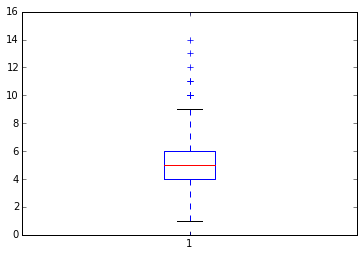
\includegraphics[height=6cm]{../fig/Tut-02-py-03-boxplot.png}
\end{center}
Como vamos a ver, dibujar un gráfico con {\tt matplotlib} es un proceso en dos etapas:
\begin{enumerate}
\item Para {\em construir} el gráfico usamos la función {\tt boxplot} del módulo {\tt matplotlib} (por eso el prefijo {\tt plt}).
\item Para {\em mostrar} el gráfico usamos la función {\tt show}, también de {\tt matplotlib}.
\end{enumerate}
Aunque al principio pueda parecer complicado, esto nos permitirá más adelante utilizar varios comandos para construir gráficos complicados combinando los resultados de esos comandos en una sóla gráfica que finalmente mostraremos con {\tt show}.

El siguiente gráfico que vamos a construir es un diagrama de barras (o columnas), que representa gráficamente la información de nuestra tabla de frecuencias. La posición sobre el eje horizontal de cada barra corresponde con uno de los valores de la primera columna de esa tabla (los valores distintos que aparecen en los datos), mientras que la altura de cada una de las barras queda determinada por la frecuencia absoluta de ese valor. Así que el código empieza identificando esas listas de valores con los nombres {\tt posiciones} y {\tt alturas}. Esto no era, desde luego, necesario, pero ayuda a mejorar la legibilidad del código. Para construir el gráfico usamos la función {\tt bar} de {\tt matplotlib} a la que, aparte de {\tt posiciones} y {\tt alturas}, hemos añadido el argumento opcional {\tt color='tan'} para modificar el color de relleno de las barras del diagrama (el color por defecto es azul oscuro). Como antes, usamos {\tt show} para mostrar el gráfico resultante.
\begin{knitrout}
\definecolor{shadecolor}{rgb}{0.969, 0.969, 0.969}\color{fgcolor}\begin{kframe}
\begin{alltt}
\hlkwd{print}\hlstd{(}\hlstr{"Diagrama de barras a partir de la tabla de frecuencias:"}\hlstd{)}
\hlstd{posiciones} \hlkwb{=} \hlstd{valoresUnicos}
\hlstd{alturas} \hlkwb{=} \hlstd{freqAbs}
\hlkwd{plt.bar}\hlstd{(posiciones, alturas,} \hlkwc{color}\hlstd{=}\hlstr{'tan'}\hlstd{)}
\hlkwd{plt.show}\hlstd{()}
\end{alltt}
\end{kframe}
\end{knitrout}
El diagrama de barras que se obtiene es este:
\begin{center}
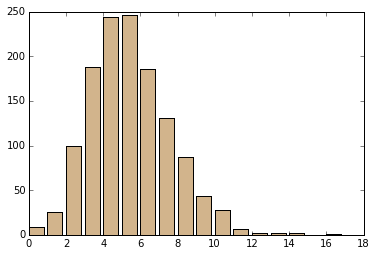
\includegraphics[height=8cm]{../fig/Tut-02-py-04-diagBarras.png}
\end{center}
Si te fijas bien, verás que los valores del eje no están correctamente centrados en las columnas del gráfico. Por el momento lo dejamos pasar. Más adelante nos iremos ocupando de este y otros detalles, para mejorar la calidad de los gráficos.

El último gráfico que vamos a construir es un histograma. Puesto que estamos tratando con una variable cuantitativa discreta, el histograma no es nuestra elección prioritaria para representar estos datos: el diagrama de barras es mejor para esta situación. Pero hecha esa advertencia, queremos aprovechar para mostra la facilidad con la que Python permite construir histogramas. El código es este:
\begin{knitrout}
\definecolor{shadecolor}{rgb}{0.969, 0.969, 0.969}\color{fgcolor}\begin{kframe}
\begin{alltt}
\hlkwd{print}\hlstd{(}\hlstr{"Histograma:"}\hlstd{)}
\hlkwd{plt.hist}\hlstd{(datos,} \hlkwc{bins}\hlstd{=}\hlkwd{len}\hlstd{(valoresUnicos),} \hlkwc{color}\hlstd{=}\hlstr{'tan'}\hlstd{)}
\hlkwd{plt.show}\hlstd{()}

\hlkwd{print}\hlstd{(linea)}
\end{alltt}
\end{kframe}
\end{knitrout}
Como ves, la función de {\tt matplotlib} responsable de construir el histograma se llama {\tt hist}. El único argumento necesario para {\tt hist} es la lista de datos. Pero podemos usar el argumento opcional {\tt bins} para indicar el número de clases en las que queremos agrupar los datos para representarlos ({\em bin} en inglés significa {\em caja, bote} o {\em compartimento}). En este caso hemos hecho que haya tantas cajas como valores distintos para que el perfil del histograma fuera bastante parecido al del diagrama de barras. Y como antes hemos cambiado el color de las barras del gráfico.
\begin{center}
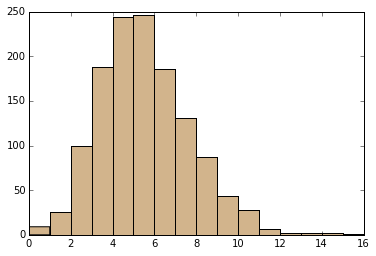
\includegraphics[height=8cm]{../fig/Tut-02-py-05-histograma.png}
\end{center}
Fijate en las diferencias y similitudes entre el diagrama de barras y el histograma.

\subsubsection*{Media aritmetica y medidas de dispersión.}
\label{tut02:subsubsec:mediaAritmeticaDispersion}



En este apartado vamos a usar funciones de {\tt numpy} para calcular rápidamente la media aritmética y varias medidas de dispersión de los datos. Empezando por la media, el cálculo usa la función {\tt mean}
\begin{knitrout}
\definecolor{shadecolor}{rgb}{0.969, 0.969, 0.969}\color{fgcolor}\begin{kframe}
\begin{alltt}
\hlkwd{print}\hlstd{(}\hlstr{"Media aritmética:"}\hlstd{)}
\hlstd{mediaAritmetica} \hlkwb{=} \hlkwd{np.mean}\hlstd{(datos)}
\hlkwd{print}\hlstd{(mediaAritmetica)}
\end{alltt}
\end{kframe}
\end{knitrout}
El resultado es:
\begin{knitrout}
\definecolor{shadecolor}{rgb}{0.969, 0.969, 0.969}\color{fgcolor}\begin{kframe}
\begin{alltt}
Media aritmética:
5.03923076923
\end{alltt}
\end{kframe}
\end{knitrout}
El módulo {\tt numpy} incluye dos funciones para calcular las medidas de dispersión, llamadas {\tt var} y {\tt std}. La primera de estas funciones sirve para calcular la varianza poblacional y la cuasivarianza muestral. Para saber cuál de ellas calculamos existe un argumento llamado {\tt ddof} (del inglés {\em delta degrees of freedom}). Ya sabes que para calcular la cuasivarianza muestral el denominador es $n - 1$, mientras que para la varianza poblacional el denominador es $n = n - 0$ (siendo $n$ el número de datos). El valor de {\tt ddof} es el valor {\em que se resta de} $n$. Por eso para la varianza poblacional usamos {\tt ddof = 0}, mientras que para la cuasivarianza muestral usamos {\tt ddof = 1}.
\begin{knitrout}
\definecolor{shadecolor}{rgb}{0.969, 0.969, 0.969}\color{fgcolor}\begin{kframe}
\begin{alltt}
\hlkwd{print}\hlstd{(}\hlstr{"Varianza poblacional"}\hlstd{)}
\hlstd{varPoblacional} \hlkwb{=} \hlkwd{np.var}\hlstd{(datos,} \hlkwc{ddof}\hlstd{=}\hlnum{0}\hlstd{)}
\hlkwd{print}\hlstd{(varPoblacional)}
\hlkwd{print}\hlstd{(}\hlstr{"Cuasivarianza muestral"}\hlstd{)}
\hlstd{cuasivarMuestral} \hlkwb{=} \hlkwd{np.var}\hlstd{(datos,} \hlkwc{ddof}\hlstd{=}\hlnum{1}\hlstd{)}
\hlkwd{print}\hlstd{(cuasivarMuestral)}
\end{alltt}
\end{kframe}
\end{knitrout}

Con la desviación típìca poblacional y la cuasivarianza muestral las cosas son muy parecidas, cambiando {\tt var} por {\tt std} (de {\em standard deviation}):
\begin{knitrout}
\definecolor{shadecolor}{rgb}{0.969, 0.969, 0.969}\color{fgcolor}\begin{kframe}
\begin{alltt}
\hlkwd{print}\hlstd{(}\hlstr{"Desviación típica poblacional"}\hlstd{)}
\hlstd{desvestPoblacional} \hlkwb{=} \hlkwd{np.std}\hlstd{(datos,} \hlkwc{ddof}\hlstd{=}\hlnum{0}\hlstd{)}
\hlkwd{print}\hlstd{(desvestPoblacional)}
\hlkwd{print}\hlstd{(}\hlstr{"Cuasidesviación típica muestral"}\hlstd{)}
\hlstd{cuasidesvestMuestral} \hlkwb{=} \hlkwd{np.std}\hlstd{(datos,} \hlkwc{ddof}\hlstd{=}\hlnum{1}\hlstd{)}
\hlkwd{print}\hlstd{(cuasidesvestMuestral)}

\hlkwd{print}\hlstd{(linea)}
\end{alltt}
\end{kframe}
\end{knitrout}
El resultado de ese código es:
\begin{knitrout}
\definecolor{shadecolor}{rgb}{0.969, 0.969, 0.969}\color{fgcolor}\begin{kframe}
\begin{alltt}
Varianza poblacional
4.71153786982
Cuasivarianza muestral
4.71516491976
Desviación típica poblacional
2.17060771901
Cuasidesviación típica muestral
2.17144305008
\end{alltt}
\end{kframe}
\end{knitrout}

Vamos a explorar algunas de las ideas que aparecen en ese programa a través de los apartados de este ejercicio.
\begin{ejercicio}
\label{tut02:ejercicio26}
\quad\\
\begin{enumerate}
\item Para empezar, ejecuta el programa en la terminal de IPython utilizando la función mágica \verb&%run&.
Recuerda que debes en primer lugar asegurarte de que tanto el fichero de código {\tt py} como el fichero de datos {\tt csv} están situados en las carpetas adecuadas. Además debes incluir el nombre del fichero de datos en el fichero de código Python para que la función \verb&read_csv& pueda hacer su trabajo.  Tras ejecutar el código y ver aparecer los resultados conseguirás que todas las variables que se definen en el código sean accesibles en esa sesión IPython. En particular la variable {\tt datos} contiene la lista de datos procedente del fichero {\tt csv}.
\item Calcula el percentil $20$ de los datos.
\item Comprueba que el valor de la media aritmética que produce el programa (y que está almacenado en la variable {\tt mediaAritmetica}) coincide con lo que obtienes dividiendo la suma de datos por {\tt n}.
\item Usa código como el del fichero {\tt Tut02-mediaVarianza-01.py} (ver pág. \pageref{fichero:Tut02-mediaVarianza-01}) para calcular la varianza y la desviación típica poblacionales y comprueba que coinciden con los resultados de {\tt numpy} (puede haber una pequeña diferencia debida al redondeo). Haz lo mismo con la cuasivarianza y la cuasidesviación típica muestrales.
\item Ejecuta de nuevo el programa (usando \verb&%run&),
pero antes de hacerlo comenta la línea
\begin{knitrout}
\definecolor{shadecolor}{rgb}{0.969, 0.969, 0.969}\color{fgcolor}\begin{kframe}
\begin{alltt}
\hlkwd{get_ipython}()\hlkwd{.magic}(\hlstr{'matplotlib inline'})
\end{alltt}
\end{kframe}
\end{knitrout}
Es decir, cámbiala a:
\begin{knitrout}
\definecolor{shadecolor}{rgb}{0.969, 0.969, 0.969}\color{fgcolor}\begin{kframe}
\begin{alltt}
\hlcom{# get_ipython().magic('matplotlib inline')}
\end{alltt}
\end{kframe}
\end{knitrout}
Acuérdate de grabar el programa con ese cambio antes de volver a ejecutarlo (y de deshacer el cambio cuando acabes este ejercicio). ¿Qué sucede ahora al ejecutar el programa? Si todo va como se espera verás aparecer una ventana gráfica con el diagrama de cajas. Para seguir avanzando debes cerrar esta ventana. Cuando lo hagas aparecerá otra ventana con el siguiente gráfico, el de barras. Al cerrar esta aparecerá el histograma y finalmente, al cerrar esta concluirá la ejecución del resto del programa. Este es el comportamiento típico de IPython cuando no se usa la orden \verb& get_ipython().magic('matplotlib inline')&. En programas que muestran un gran número de gráficos eso puede resultar molesto, así que es bueno que conozcas las opciones de las que dispones.
\item Dibuja un gráfico de barras en el que la altura de las barras corresponda a las  frecuencias acumuladas en lugar de las absolutas. Más adelante en el curso volveremos sobre las diferencias entre estos dos tipos de gráficos.
\end{enumerate}
%Solución en la página \pageref{tut02:ejercicio26:sol}.
\qed
\end{ejercicio}

\section{Más operaciones con listas.}
\label{tut02:sec:masOperacionesListas}

\subsection{Números aleatorios.}
\label{tut02:subsec:numerosAleatorios}

En el Tutorial-01 vimos como generar números (pseudo)aleatorios con Calc. Y en el Capítulo \ref{curso-cap:Probabilidad} de la teoría del curso se usan esos números para hacer varios experimentos relacionados con las probabilidades, en situaciones bastante elementales. Para prepararnos, vamos a aprender a hacer lo mismo con Python. Como veremos, vamos a poder ir mucho más allá de lo que resulta viable hacer con Calc.

Muchas de las funciones que vamos a utilizar se ubican en el módulo {\tt random}. Así que empezaremos importándolo.
\begin{knitrout}
\definecolor{shadecolor}{rgb}{0.969, 0.969, 0.969}\color{fgcolor}\begin{kframe}
\begin{alltt}
import random as rnd
\end{alltt}
\end{kframe}
\end{knitrout}
La primera de las funciones de este módulo que vamos a examinar es la función {\tt randrange}, que nos permitirá simular situaciones sencillas como el lanzamiento de un dado. Vamos a verla en acción en la terminal de IPython. Ten en cuenta que cuando tú ejecutes este código obtendrás valores distintos de los que aparecen aquí:
\begin{knitrout}
\definecolor{shadecolor}{rgb}{0.969, 0.969, 0.969}\color{fgcolor}\begin{kframe}
\begin{alltt}
In [1]: import random as rnd

In [2]: \hlkwd{rnd.randrange}(1, 7)
Out[2]: 2

In [3]: \hlkwd{rnd.randrange}(1, 7)
Out[3]: 5

In [4]: \hlkwd{rnd.randrange}(1, 7)
Out[4]: 5

In [5]: \hlkwd{rnd.randrange}(1, 7)
Out[5]: 6

In [6]: \hlkwd{rnd.randrange}(1, 7)
Out[6]: 3

In [7]: \hlkwd{rnd.randrange}(1, 7)
Out[7]: 1
\end{alltt}
\end{kframe}
\end{knitrout}
Como ves, cada vez que ejecutamos la función se obtiene un número entero del 1 al 6. Como en otros casos que hemos visto en Python, usamos {\tt (1, 7)} pero el último número entero de ese intervalo (el 7) se excluye. En general, al escribir {\tt rnd.randrange(a, b)} obtenemos números entre {\tt a} y {\tt b-1}. Por ejemplo, si en lugar de lanzar un dado queremos sacar cartas (sin reemplazamiento) de una baraja de 48 cartas, entonces podemos representar las cartas de la baraja con los números del $1$ al $48$ y bastaría con usar {\tt randrange} así:
\begin{knitrout}
\definecolor{shadecolor}{rgb}{0.969, 0.969, 0.969}\color{fgcolor}\begin{kframe}
\begin{alltt}
In [1]: import random as rnd

In [2]: \hlkwd{rnd.randrange}(1, 49)
Out[2]: 27

In [3]: \hlkwd{rnd.randrange}(1, 49)
Out[3]: 13

In [4]: \hlkwd{rnd.randrange}(1, 49)
Out[4]: 36

In [5]: \hlkwd{rnd.randrange}(1, 49)
Out[5]: 42

In [6]: \hlkwd{rnd.randrange}(1, 49)
Out[6]: 6
\end{alltt}
\end{kframe}
\end{knitrout}
Aunque podemos usar la función así para fabricar unos pocos valores, lo que de verdad vamos a vecesitar es la capacidad de hacer simulaciones en las que un experimento se repita cientos o miles de veces. Vamos a combinar la función {\tt randrange} con la comprensión de listas para simular 100 tiradas de un dado:
\begin{knitrout}
\definecolor{shadecolor}{rgb}{0.969, 0.969, 0.969}\color{fgcolor}\begin{kframe}
\begin{alltt}
In [1]: import random as rnd

In [2]: dado100 = [\hlkwd{rnd.randrange}(1, 7) for _ in \hlkwd{range}(0, 100)]

In [3]: \hlkwd{print}(dado100)
[5, 5, 4, 6, 6, 6, 4, 4, 6, 5, 1, 6, 6, 6, 3, 2, 4, 6, 5, 6, 2, 5, 1, 2, 6, 2, 6,
4, 3, 2, 5, 1, 1, 5, 1, 3, 3, 6, 5, 6, 6, 5, 6, 1, 6, 3, 4, 1, 6, 1, 4, 2, 5, 2, 5,
1, 3, 4, 3, 4, 6, 5, 2, 4, 2, 5, 3, 2, 3, 4, 1, 1, 3, 4, 6, 3, 4, 1, 6, 3, 5, 2, 2,
1, 3, 3, 2, 2, 2, 5, 2, 4, 3, 2, 2, 3, 5, 6, 5, 3]
\end{alltt}
\end{kframe}
\end{knitrout}
Un detalle técnico: fíjate en que hemos escrito \verb&for _ in range(0, 100)&, usando un guión bajo \verb&_& para representar la variable auxiliar del {\tt for}. También podríamos haber escrito {\tt for item in range(0, 100)}, usando una variable auxiliar {\tt item}, y el resultado habría sido el mismo. Pero los programadores de Python usan a menudo ese convenio de notación llamando \verb&_& a la variable auxiliar {\em cuando esa variable no se utiliza en ningún otro punto del código y es simplemente un contador de iteraciones}.

Hasta ahora, hemos visto ejemplos en los que extraíamos valores aleatorios de intervalos que empiezan en $1$, como {\tt 1:6}, y {\tt 1:48}. Naturalmente, podemos aplicar {\tt randrange} a un intervalo como {\tt 161:234}. Otras veces, en cambio, nos sucederá que tenemos una lista, como esta lista {\tt edades}:
{\small
\begin{knitrout}
\definecolor{shadecolor}{rgb}{0.969, 0.969, 0.969}\color{fgcolor}\begin{kframe}
\begin{alltt}
edades = [22, 21, 18, 19, 17, 21, 18, 20, 17, 18, 17, 22, 20, 19, 18, 19, 18, 22, 20, 19]
\end{alltt}
\end{kframe}
\end{knitrout}
}
y lo que queremos es extraer algunos  de estos valores al azar; pongamos por ejemplo, que queremos extraer $7$ elementos. Para hacer eso, si queremos muestreo sin reemplazamiento podemos usar la función {\tt sample} del módulo {\tt random}. Veamos como:
{\small
\begin{knitrout}
\definecolor{shadecolor}{rgb}{0.969, 0.969, 0.969}\color{fgcolor}\begin{kframe}
\begin{alltt}
In [1]: import random as rnd

In [2]: edades = [22, 21, 18, 19, 17, 21, 18, 20, 17, 18, 17, 22, 20, 19, 18, 19, 18, 22, 20, 19]

In [3]: edadesAzar_NoRemp = \hlkwd{rnd.sample}(edades, 7)

In [4]: \hlkwd{print}(edadesAzar_NoRemp)
[18, 21, 17, 20, 18, 20, 17]
\end{alltt}
\end{kframe}
\end{knitrout}
}
En cambio, si lo que queremos es extraer elementos con reemplazamiento entonces podemos usar la función {\tt choice}. Esta función permite extraer un único elemento al azar de una lista. Para extraer más de uno la combinamos con la comprensión de listas, de la misma forma que hicimos para las tiradas del dado. Por ejemplo, para extraer 100 edades al azar de la lista dada hacemos esto (necesariamente con reemplazamiento, claro):
\begin{knitrout}
\definecolor{shadecolor}{rgb}{0.969, 0.969, 0.969}\color{fgcolor}\begin{kframe}
\begin{alltt}
In [5]: edadesAzar_Remp = [\hlkwd{rnd.choice}(edades) for _ in \hlkwd{range}(0, 100)]

In [6]: \hlkwd{print}(edadesAzar_Remp)
[17, 20, 19, 17, 20, 18, 19, 19, 19, 17, 18, 18, 19, 18, 20, 19, 17, 22, 19, 17,
20, 18, 22, 18, 21, 20, 18, 22, 20, 22, 22, 19, 18, 20, 20, 19, 21, 21, 22, 22,
18, 19, 20, 20, 21, 18, 22, 17, 22, 19, 20, 17, 18, 21, 18, 17, 21, 21, 22, 22,
22, 20, 22, 17, 21, 19, 17, 18, 17, 18, 22, 18, 21, 19, 19, 22, 22, 18, 22, 19,
21, 19, 19, 18, 18, 18, 20, 19, 19, 21, 22, 17, 22, 18, 19, 18, 20, 22, 18, 18]
\end{alltt}
\end{kframe}
\end{knitrout}
Fíjate en que, en este caso, la lista original ya contiene elementos repetidos. Así que, independientemente de que el muestreo sea con reemplazamiento o sin él, siempre podemos obtener valores repetidos. Tanto {\tt sample} como {\tt choice} eligen al azar {\em posiciones} dentro de la lista {\tt edades}, y no los {\em valores} que ocupan esas posiciones.  Para entender esto un poco mejor, mira lo que sucede al ejecutar este código, en el que usamos {\tt choice} para extraer 100 valores aleatorios de una lista que tiene el número $1$ repetido $9$ veces y un único $2$:
\begin{knitrout}
\definecolor{shadecolor}{rgb}{0.969, 0.969, 0.969}\color{fgcolor}\begin{kframe}
\begin{alltt}
In [7]: muchosUnos = [1,1,1,1,1,1,1,1,1,2]

In [8]: muestra = [\hlkwd{rnd.choice}(muchosUnos) for _ in \hlkwd{range}(0, 100)]

In [9]: \hlkwd{print}(muestra)
[1, 1, 1, 1, 1, 1, 1, 1, 1, 1, 2, 1, 2, 2, 1, 1, 2, 1, 1, 1, 1, 2, 1, 1, 1, 1,
1, 1, 1, 1, 1, 1, 1, 1, 1, 1, 1, 1, 1, 1, 1, 1, 2, 1, 1, 1, 1, 1, 1, 1, 1, 1,
2, 1, 1, 1, 1, 1, 1, 1, 1, 1, 1, 1, 1, 1, 1, 2, 2, 1, 1, 1, 1, 1, 2, 1, 1, 1,
1, 1, 1, 1, 1, 1, 1, 2, 2, 1, 1, 1, 1, 1, 1, 1, 1, 1, 1, 1, 1, 1]
\end{alltt}
\end{kframe}
\end{knitrout}
Hay otra función del módulo {\tt random} que también usaremos a menudo, la función {\tt shuffle}, que en inglés significa {\em barajar}. Y como su nombre indica, lo que esta función hace es barajar o reordenar en orden aleatorio los elementos de una lista. Por ejemplo:
\begin{knitrout}
\definecolor{shadecolor}{rgb}{0.969, 0.969, 0.969}\color{fgcolor}\begin{kframe}
\begin{alltt}
In [10]: lista = [1, 2, 3, 4, 5, 6, 7, 8]

In [11]: \hlkwd{rnd.shuffle}(lista)

In [12]: lista
Out[12]: [5, 3, 6, 2, 7, 1, 8, 4]
\end{alltt}
\end{kframe}
\end{knitrout}
Fíjate en que la reordenación es {\em in situ}. Si no quieres modificar la lista original, puedes usar {\tt sample} así:
\begin{knitrout}
\definecolor{shadecolor}{rgb}{0.969, 0.969, 0.969}\color{fgcolor}\begin{kframe}
\begin{alltt}
In [13]: lista = [1, 2, 3, 4, 5, 6, 7, 8]

In [14]: \hlkwd{rnd.sample}(lista, \hlkwd{len}(lista))
Out[14]: [1, 5, 4, 8, 6, 7, 2, 3]

In [15]: lista
Out[15]: [1, 2, 3, 4, 5, 6, 7, 8]
\end{alltt}
\end{kframe}
\end{knitrout}
Como ves, una muestra obtenida con {\tt sample} de longitud igual a la de la lista original es simplemente una reordenación aleatoria de la lista. Pero este método no afecta a la lista original.

Estas tres funciones {\tt sample, choice, shuffle} se aplican de la misma forma a listas de cadenas de caracteres, como ilustran estos ejemplos:
\begin{knitrout}
\definecolor{shadecolor}{rgb}{0.969, 0.969, 0.969}\color{fgcolor}\begin{kframe}
\begin{alltt}
In [22]: continentes = [\hlstr{"América"}, \hlstr{"Asia"}, \hlstr{"Europa"}, \hlstr{"África"}, \hlstr{"Oceanía"}, \hlstr{"Antártida"}]

In [23]: \hlkwd{rnd.sample}(continentes, 3)
Out[23]: [\hlstr{'América'}, \hlstr{'Oceanía'}, \hlstr{'Europa'}]

In [24]: muestra = [\hlkwd{rnd.choice}(continentes) for _ in \hlkwd{range}(0, 20)]

In [25]: \hlkwd{print}(muestra)
[\hlstr{'Europa'}, \hlstr{'África'}, \hlstr{'Europa'}, \hlstr{'Antártida'}, \hlstr{'América'}, \hlstr{'Europa'}, \hlstr{'Oceanía'}, \hlstr{'Asia'},
\hlstr{'Europa'}, \hlstr{'América'}, \hlstr{'Asia'}, \hlstr{'América'}, \hlstr{'Europa'}, \hlstr{'Europa'}, \hlstr{'África'}, \hlstr{'Oceanía'},
\hlstr{'Oceanía'}, \hlstr{'América'}, \hlstr{'África'}, \hlstr{'África'}]

In [26]: \hlkwd{rnd.shuffle}(continentes)

In [27]: \hlkwd{print}(continentes)
[\hlstr{'Antártida'}, \hlstr{'Europa'}, \hlstr{'África'}, \hlstr{'Oceanía'}, \hlstr{'Asia'}, \hlstr{'América'}]
\end{alltt}
\end{kframe}
\end{knitrout}

\subsubsection*{Usando {\tt numpy} para fabricar números aleatorios.}
\label{tut02:subsubsec:usandoNumpyNumerosAleatorios}

Aunque las funciones del módulo {\tt random} son, por el momento, suficientes para nuestras necesidades, es conveniente que conozcas algunas posibilidades que ofrece {\tt numpy}, entre otras razones porque puedes encontrártelas en el código de otras personas. A lo largo del curso iremos presentando cada vez más de estas herramientas. Para empezar podemos usar la función {\tt random.choice} de {\tt numpy}, que ilustra este ejemplo:
\begin{knitrout}
\definecolor{shadecolor}{rgb}{0.969, 0.969, 0.969}\color{fgcolor}\begin{kframe}
\begin{alltt}
In [16]: import numpy as np

In [17]: edades = [22, 21, 18, 19, 17, 21, 18, 20, 17, 18, 17, 22, 20, 19,
18, 19, 18, 22, 20, 19]

In [18]: \hlkwd{np.random.choice}(edades, size=100, replace=True)
Out[18]:
\hlkwd{array}([22, 19, 19, 22, 18, 18, 20, 18, 18, 21, 18, 19, 17, 20, 20, 22, 22,
       22, 17, 22, 18, 18, 18, 19, 18, 20, 18, 22, 19, 17, 22, 20, 21, 18,
       17, 17, 22, 18, 18, 19, 19, 21, 18, 18, 17, 19, 19, 19, 17, 18, 17,
       19, 17, 19, 20, 18, 22, 19, 21, 21, 17, 17, 22, 18, 19, 21, 19, 18,
       19, 21, 17, 21, 18, 19, 17, 21, 20, 20, 22, 22, 22, 20, 22, 19, 17,
       18, 20, 19, 18, 20, 18, 20, 22, 22, 22, 21, 21, 19, 20, 20])
\end{alltt}
\end{kframe}
\end{knitrout}
El resultado es similar a lo que obteníamos antes combinando la función {\tt choice} del módulo {\tt random} con la comprensión de listas. Se obtiene una muestra aleatoria con reemplazamiento de los elementos de la lista original. Hemos dejado la salida tal cual para que puedas observar que el resultado no es una lista, sino un objeto {\tt ndarray} de {\tt numpy}.

\subsection{Conjuntos.}
\label{tut02:subsec:conjuntos}

Aunque las listas han tenido en este tutorial un papel protagonista, ya hemos anunciado que a lo largo del curso irán apareciendo otras estructuras de datos que resultan necesarias para facilitar nuestro trabajo. En particular, al estudiar la probabilidad necesitaremos trabajar con {\sf conjuntos}. La mayor diferencia entre un conjunto y una lista es que el conjunto no puede contener elementos repetidos. Para definir un conjunto podemos enumerar sus elementos entre llaves. Usamos la terminal de IPython definimos y mostramos un conjunto {\tt A}:
\begin{knitrout}
\definecolor{shadecolor}{rgb}{0.969, 0.969, 0.969}\color{fgcolor}\begin{kframe}
\begin{alltt}
In [1]: A = \{4, -3, 1, 2, 5, 4, 6, 7, 1, 2\}

In [2]: \hlkwd{print}(A)
\{1, 2, 4, 5, 6, 7, -3\}
\end{alltt}
\end{kframe}
\end{knitrout}
Fíjate en que Python ha eliminado automáticamente los elementos repetidos de {\tt A}. De paso los ha reordenado de alguna manera extraña. Esa es la otra propiedad importante de los conjuntos de Python: el orden no es importante y a menudo resulta difícil o imposible predecir el orden en que Python colocará los elementos en un conjunto. Si tratamos de acceder a ellos como en una lista sucede esto:
\begin{knitrout}
\definecolor{shadecolor}{rgb}{0.969, 0.969, 0.969}\color{fgcolor}\begin{kframe}
\begin{alltt}
In [3]: A[0:4]
\hlkwd{Traceback} (most recent call last):

  File \hlstr{"<ipython-input-3-8c229c82880a>"}, line 1, in <module>
    A[0:4]

TypeError: \hlstr{'set'} object is not subscriptable
\end{alltt}
\end{kframe}
\end{knitrout}
Como ves Python nos recuerda {\em amablemente} que un conjunto no es como una lista. Pero eso no significa que no podamos hacer operaciones sobre los elementos del conjunto, de forma similar a lo que hacíamos en las comprensiones de lista. Por ejemplo, podemos elevar todos los elementos al cuadrado:
\begin{knitrout}
\definecolor{shadecolor}{rgb}{0.969, 0.969, 0.969}\color{fgcolor}\begin{kframe}
\begin{alltt}
In [4]: B = \{item**2 for item in A\}

In [5]: \hlkwd{print}(B)
\{1, 4, 36, 9, 16, 49, 25\}
\end{alltt}
\end{kframe}
\end{knitrout}
Por cierto, aquí tienes una nueva oportunidad de ver lo que decíamos sobre lo difícil de predecir el orden de los elementos.

Al igual que hemos hecho una {\sf comprensión de conjuntos}, podemos usar los elementos de un conjunto en un bucle {\tt for}, como hacemos aquí:
\begin{knitrout}
\definecolor{shadecolor}{rgb}{0.969, 0.969, 0.969}\color{fgcolor}\begin{kframe}
\begin{alltt}
for item in A:
  \hlkwd{print}(\hlstr{"El siguiente elemento de A es \{0\} y su cuadrado es \{1\}"}\hlkwd{.format}(item, item**2))
\end{alltt}
\end{kframe}
\end{knitrout}
Al ejecutar este código en la terminal  de IPython se obtiene:
\begin{knitrout}
\definecolor{shadecolor}{rgb}{0.969, 0.969, 0.969}\color{fgcolor}\begin{kframe}
\begin{alltt}
El siguiente elemento de A es 1 y su cuadrado es 1
El siguiente elemento de A es 2 y su cuadrado es 4
El siguiente elemento de A es 4 y su cuadrado es 16
El siguiente elemento de A es 5 y su cuadrado es 25
El siguiente elemento de A es 6 y su cuadrado es 36
El siguiente elemento de A es 7 y su cuadrado es 49
El siguiente elemento de A es -3 y su cuadrado es 9
\end{alltt}
\end{kframe}
\end{knitrout}
La propiedad de no contener repeticiones es de hecho la primera utilidad que encontramos de la idea de conjunto. Si tenemos una lista de valores y queremos saber cuántos y cuáles son los valores distintos que aparecen en esa lista, podemos convertir la lista en un conjunto. Eso es lo que se hace en el código de este ejemplo:
\begin{knitrout}
\definecolor{shadecolor}{rgb}{0.969, 0.969, 0.969}\color{fgcolor}\begin{kframe}
\begin{alltt}
import random as rnd
datos = [\hlkwd{rnd.randrange}(0, 100) for _ in \hlkwd{range}(0, 60)]
\hlkwd{print}(\hlstr{"Los 60 datos son:"} )
\hlkwd{print}(datos)
valoresUnicos = \hlkwd{set}(datos)
\hlkwd{print}(\hlstr{"Entre los datos hay \{0\} valores únicos que son:"}\hlkwd{.format}(\hlkwd{len}(valoresUnicos)))
\hlkwd{print}(valoresUnicos)
\end{alltt}
\end{kframe}
\end{knitrout}
El resultado al ejecutarlo es:
\begin{knitrout}
\definecolor{shadecolor}{rgb}{0.969, 0.969, 0.969}\color{fgcolor}\begin{kframe}
\begin{alltt}
Los 60 datos son:
[47, 31, 99, 60, 28, 86, 86, 41, 56, 18, 13, 45, 66, 11, 24, 98, 60, 54, 94, 3,
 90, 64, 21, 87, 91, 22, 85, 12, 49, 90, 33, 8, 46, 38, 28, 26, 17, 83, 86, 17,
 71, 0, 66, 96, 2, 22, 33, 49, 50, 2, 64, 3, 47, 62, 82, 80, 17, 72, 0, 80]
Entre los datos hay 43 valores únicos que son:
\{0, 2, 3, 8, 11, 12, 13, 17, 18, 21, 22, 24, 26, 28, 31, 33, 38, 41, 45, 46, 47, 49,
 50, 54, 56, 60, 62, 64, 66, 71, 72, 80, 82, 83, 85, 86, 87, 90, 91, 94, 96, 98, 99\}
\end{alltt}
\end{kframe}
\end{knitrout}
Fíjate especialmente en estos dos detalles:
\begin{enumerate}
\item La línea:
\begin{knitrout}
\definecolor{shadecolor}{rgb}{0.969, 0.969, 0.969}\color{fgcolor}\begin{kframe}
\begin{alltt}
datos = [\hlkwd{rnd.randrange}(0, 100) for _ in \hlkwd{range}(0, 60)]
\end{alltt}
\end{kframe}
\end{knitrout}
sirve para generar 60 números al azar entre 0 y 99. Es un truco que repetiremos más veces en el curso, así que asegúrate de que entiendes como funciona.
\item La función {\tt set} convierte una lista en un conjunto y es, de hecho, la que elimina las repeticiones.
\end{enumerate}
De la misma forma, la función {\tt list} permite convertir un conjunto en una lista y de esa forma recuperar la posibilidad de ordenar los elementos, seleccionar parte de ellos, etc. Por ejemplo, al ejecutar:
\begin{knitrout}
\definecolor{shadecolor}{rgb}{0.969, 0.969, 0.969}\color{fgcolor}\begin{kframe}
\begin{alltt}
\hlstd{unicos} \hlkwb{=} \hlkwd{list}\hlstd{(valoresUnicos)}
\hlkwd{print}\hlstd{(unicos)}
\hlkwd{print}\hlstd{(unicos[}\hlnum{4}\hlopt{:}\hlnum{12}\hlstd{])}
\end{alltt}
\end{kframe}
\end{knitrout}
se obtiene:
\begin{knitrout}
\definecolor{shadecolor}{rgb}{0.969, 0.969, 0.969}\color{fgcolor}\begin{kframe}
\begin{alltt}
[0, 1, 2, 3, 6, 12, 18, 20, 26, 27, 29, 31, 33, 34, 36, 38, 45, 47, 48, 49, 52, 55,
 56, 57, 59, 61, 64, 65, 66, 67, 74, 76, 77, 78, 80, 83, 84, 88, 92, 95, 97, 98]
[6, 12, 18, 20, 26, 27, 29, 31]
\end{alltt}
\end{kframe}
\end{knitrout}
Nos hemos asomado apenas a las posibilidades que ofrece el trabajo con conjuntos en Python. Tendremos ocasión más adelante de ver cómo se pueden realizar muchas de las operaciones típicas: uniones, intersecciones, diferencias de conjuntos, etc.

\subsection{Bucles for anidados.}
\label{tut02:subsec:buclesForAnidados}

A veces nos encontramos con esta situación: tenemos una tabla de frecuencias absolutas de un conjunto de datos, pero no tenemos la lista original con los datos. No es una situación infrecuente: a veces al leer un artículo los datos aparecen resumidos en forma de tabla de frecuencias. Y sin embargo, muchas de las operaciones que vamos a realizar asumen que el punto de partida es una lista de datos, repetidos tantas veces como corresponda a su frecuencia. Si antes aprendimos a fabricar la tabla de frecuencias absolutas de una lista de datos, lo que necesitamos ahora es la operación inversa: pasar de la tabla de frecuencias a la lista de datos. Es importante darse cuenta de que en realidad la tabla de frecuencias, por si misma, no permite recuperar por completo la lista original: el orden de los elementos se habrá perdido. Pero no es menos cierto que el orden no juega ningún papel en muchas operaciones estadísticas, como el cálculo de medias, medianas, varianzas, etc.

Para empezar vamos a suponer que los disintos valores y sus frecuencias están disponibles en dos listas:
\begin{knitrout}
\definecolor{shadecolor}{rgb}{0.969, 0.969, 0.969}\color{fgcolor}\begin{kframe}
\begin{alltt}
valores = [2,3,5,8,13]
frecuencias = [5,7,12,2,14]
\end{alltt}
\end{kframe}
\end{knitrout}
Así pues, por ejemplo el valor $5$ aparece $12$ en los datos originales. Para reconstruir la lista de datos con repeticiones podemos aplicar esta receta en pseudocódigo:
\begin{knitrout}
\definecolor{shadecolor}{rgb}{0.969, 0.969, 0.969}\color{fgcolor}\begin{kframe}
\begin{alltt}
Crear una lista datos, inicialmente vacía.
Repetir esto para cada posición pos de la lista de valores:
  Repetir esto un número de veces igual a frecuencias[pos]:
    Anadir valores[pos] a la lista datos.
\end{alltt}
\end{kframe}
\end{knitrout}
Y la traducción en código es esta:
\begin{knitrout}
\definecolor{shadecolor}{rgb}{0.969, 0.969, 0.969}\color{fgcolor}\begin{kframe}
\begin{alltt}
datos = []
for i in \hlkwd{range}(0, \hlkwd{len}(valores)):
  for _ in \hlkwd{range}(0, frecuencias[i]):
    \hlkwd{datos.append}(valores[i])
\hlkwd{print}(datos)
\end{alltt}
\end{kframe}
\end{knitrout}
Como ves, tenemos dos bucles {\tt for} anidados: hay que hacer algo para cada posición de la lista valor, así que en el primer bucle o {\sf bucle exterior}  usamos un contador {\tt i} para recorrer la lista de valores. Pero es que además lo que hay que hacer para cada posición también es un bucle: tenemos que repetir ese valor las veces que nos indica la frecuencia correspondiente. Por eso hay un {segundo bucle, o bucle interno} en el que hacemos algo una cierta cantidad de veces. El contador de este bucle no se usa para ninguna otra operación aparte de llevar la cuenta del número veces: por eso lo llamamos simplemente \verb&_&.  Fíjate además en que el número de iteraciones del bucle interno no es constante: depende del valor de {\tt i}; es decir, depende de en qué iteración del bucle exterior nos encontramos.

Veamos cómo funciona esto en la terminal de IPython (hemos copiado los bucles {\tt for} anidados como un bloque de código, como ya aprendimos a hacer):
\begin{knitrout}
\definecolor{shadecolor}{rgb}{0.969, 0.969, 0.969}\color{fgcolor}\begin{kframe}
\begin{alltt}
In [1]: valores = [2,3,5,8,13]

In [2]: frecuencias = [5,7,12,2,14]

In [3]: datos = []

In [4]: for i in \hlkwd{range}(0, \hlkwd{len}(valores)):
   ...:   for _ in \hlkwd{range}(0, frecuencias[i]):
   ...:     \hlkwd{datos.append}(valores[i])
   ...:

In [5]: \hlkwd{print}(datos)
[2, 2, 2, 2, 2, 3, 3, 3, 3, 3, 3, 3, 5, 5, 5, 5, 5, 5, 5, 5, 5, 5, 5, 5, 8, 8, 13,
13, 13, 13, 13, 13, 13, 13, 13, 13, 13, 13, 13, 13]
\end{alltt}
\end{kframe}
\end{knitrout}
El resultado, como ves, es el deseado: la lista expandida de datos correspondiente a la tabla de frecuencias.

Tal vez te preguntes: ¿se puede hacer lo mismo con una comprensión de listas? Y la respuesta es afirmativa:
{\small
\begin{knitrout}
\definecolor{shadecolor}{rgb}{0.969, 0.969, 0.969}\color{fgcolor}\begin{kframe}
\begin{alltt}
In [6]: datos = [valores[i] for i in \hlkwd{range}(0, \hlkwd{len}(valores)) for _ in \hlkwd{range}(0, frecuencias[i])]

In [7]: \hlkwd{print}(datos)
[2, 2, 2, 2, 2, 3, 3, 3, 3, 3, 3, 3, 5, 5, 5, 5, 5, 5, 5, 5, 5, 5, 5, 5, 8, 8, 13,
13, 13, 13, 13, 13, 13, 13, 13, 13, 13, 13, 13, 13]
\end{alltt}
\end{kframe}
\end{knitrout}
}
Como ves, el orden de escritura de izquierda a derecha de los bucles en esta versión se corresponde con el orden de arriba hacia abajo en los bucles {\tt for} anidados. En cualquier caso, el resultado es el mismo. A menudo la elección entre las dos formas de proceder es una cuestión de preferencias personales. Muchos programadores opinan que los bucles {\tt for} anidados son en general más legibles, pero otros muchos sostienen que la comprensión anidada de listas es la opción {\em más pythonica}. No vamos a discutir por esto, desde luego. Recuerda en cualquier caso la directriz general que hemos visto anteriormente: las comprensiones pueden ser la forma natural de {\em fabricar objetos} (como en el caso que nos ocupa), mientras que los bucles {\em for} son la forma natural de describir {\em acciones}.

\subsection{Listas de cadenas de texto. }

Vamos a comentar muy brevemente algunas funciones del módulo {\tt string} que nos resultarán útiles en algunos ejemplos y ejercicios. Este módulo contiene varios objetos que son simplemente cadenas de caracteres con las letras del alfabeto (las que usa el idioma inglés, no incluye acentos ni la ñ) en mayúsculas, minúsculas o ambas conjuntamente:
\begin{knitrout}
\definecolor{shadecolor}{rgb}{0.969, 0.969, 0.969}\color{fgcolor}\begin{kframe}
\noindent
\ttfamily
\hlstd{}\hlkwa{import\ }\hlstd{string}\hspace*{\fill}\\
\hlkwa{print}\hlstd{}\hlopt{(}\hlstd{string}\hlopt{.}\hlstd{ascii\textunderscore lowercase}\hlopt{)}\hspace*{\fill}\\
\hlstd{}\hlkwa{print}\hlstd{}\hlopt{(}\hlstd{string}\hlopt{.}\hlstd{ascii\textunderscore uppercase}\hlopt{)}\hspace*{\fill}\\
\hlstd{}\hlkwa{print}\hlstd{}\hlopt{(}\hlstd{string}\hlopt{.}\hlstd{ascii\textunderscore letters}\hlopt{)}\hlstd{}\hspace*{\fill}
\mbox{}
\normalfont

\begin{verbatim}
## abcdefghijklmnopqrstuvwxyz
## ABCDEFGHIJKLMNOPQRSTUVWXYZ
## abcdefghijklmnopqrstuvwxyzABCDEFGHIJKLMNOPQRSTUVWXYZ
\end{verbatim}
\end{kframe}
\end{knitrout}
Como decíamos estos objetos resultan interesantes en algunos ejemplos, cuando se combinan con las funciones aleatorias que hemos visto antes. Te proponemos un ejercicio para practicar esto:
\begin{ejercicio}
\label{tut02:ejercicio27}
\quad\\
\begin{enumerate}
\item Vamos a fabricar un generador de contraseñas aleatorias. Usa las cadenas de caracteres para escribir un programa que genere contraseñas aleatorias de longitud 20 formadas por letras mayusculas, minúsculas y digitos del 0 al 9.
\item ¿Puedes modificar ese programa para garantizar que las contraseñas contienen al menos: una mayúscula, una minñuscula y un dígito?
\end{enumerate}
%Solución en la página \pageref{tut02:ejercicio27:sol}.
\qed
\end{ejercicio}

\subsection{Números pseudoaleatorios, pero ``reproducibles'': la función {\tt seed}.}
\label{tut02:subsec:numerosAleatoriosReproduciblesSeed}

En la  Sección \ref{tut02:subsec:numerosAleatorios} (pág. \pageref{tut02:subsec:numerosAleatorios}) hemos lanzado 100 veces un dado,  ejecutando este código en IPython (recuerda que hemos importado {\tt random} con el alias {\tt rnd}):
\begin{knitrout}
\definecolor{shadecolor}{rgb}{0.969, 0.969, 0.969}\color{fgcolor}\begin{kframe}
\begin{alltt}
dado100 = [\hlkwd{rnd.randrange}(1, 7) for _ in \hlkwd{range}(0, 100)]
\end{alltt}
\end{kframe}
\end{knitrout}
Un inconveniente de trabajar con números aleatorios es que los resultados del lector serán diferentes de los nuestros y, de hecho, serán diferentes cada vez que ejecutes la función {\tt randrange}. Los números aleatorios se utilizan mucho, por ejemplo, para hacer simulaciones. Y si queremos hacer una de esas simulaciones, y compartirla con otras personas, de manera que puedan {\em verificar} nuestros resultados, entonces necesitamos:
\begin{itemize}
  \item Que los números sean aleatorios, en el sentido de que nosotros no los hemos elegido, sino que son el resultado de un {\em sorteo}.
  \item Pero que los resultados del sorteo queden registrados de alguna manera, para que otros puedan reproducirlos.
\end{itemize}
Afortunadamente (en este caso), como ya dijimos, los números que produce un ordenador no son aleatorios, sino pseudoaleatorios. Y para lo que aquí nos ocupa, eso es una ventaja. Hay una función del módulo {\tt random}, llamada {\sf seed}, que permite decirle a Python que queremos hacer exactamente esto: generar números aleatorios reproducibles. Concretamente, para ver funciona como esto, probemos a ejecutar varias veces el código anterior en IPython:
\begin{knitrout}
\definecolor{shadecolor}{rgb}{0.969, 0.969, 0.969}\color{fgcolor}\begin{kframe}
\begin{alltt}
In [1]: import random as rnd

In [2]: dado100 = [\hlkwd{rnd.randrange}(1, 7) for _ in \hlkwd{range}(0, 100)]

In [3]: \hlkwd{print}(dado100)
[2, 6, 3, 4, 1, 1, 5, 6, 6, 1, 2, 1, 3, 6, 5, 1, 2, 6, 1, 1, 4, 1, 1, 1, 1, 3, 2,
2, 2, 5, 5, 1, 3, 1, 2, 5, 6, 2, 1, 5, 2, 4, 3, 1, 3, 5, 5, 5, 2, 5, 1, 1, 3, 1,
5, 2, 3, 3, 5, 4, 4, 1, 2, 2, 4, 3, 3, 3, 4, 5, 2, 2, 1, 4, 4, 2, 1, 1, 4, 2, 3,
2, 6, 4, 6, 6, 5, 4, 5, 3, 3, 2, 3, 2, 6, 5, 3, 2, 3, 5]

In [4]: dado100 = [\hlkwd{rnd.randrange}(1, 7) for _ in \hlkwd{range}(0, 100)]

In [5]: \hlkwd{print}(dado100)
[6, 1, 3, 4, 3, 3, 4, 4, 1, 6, 1, 4, 4, 1, 5, 6, 4, 1, 5, 2, 4, 6, 3, 1, 1, 5, 4,
1, 4, 6, 2, 1, 2, 5, 2, 1, 2, 4, 1, 3, 2, 6, 1, 6, 5, 6, 2, 5, 4, 3, 1, 4, 1, 3,
3, 6, 5, 6, 2, 2, 5, 4, 2, 1, 6, 1, 4, 2, 3, 5, 3, 2, 1, 3, 4, 2, 6, 3, 2, 6, 1,
6, 5, 2, 3, 3, 3, 3, 1, 4, 5, 4, 6, 6, 3, 6, 4, 5, 5, 2]
\end{alltt}
\end{kframe}
\end{knitrout}
Como esperábamos, cada vez se obtiene una lista distinta. Vamos a repetir esto, pero ahora ejecutaremos la función {\tt seed} cada vez, antes de llamar a {\tt randrange}:
\begin{knitrout}
\definecolor{shadecolor}{rgb}{0.969, 0.969, 0.969}\color{fgcolor}\begin{kframe}
\begin{alltt}
In [6]: \hlkwd{rnd.seed}(2016)

In [7]: dado100 = [\hlkwd{rnd.randrange}(1, 7) for _ in \hlkwd{range}(0, 100)]

In [8]: \hlkwd{print}(dado100)
[6, 4, 5, 3, 6, 6, 1, 3, 2, 1, 4, 4, 1, 3, 2, 2, 3, 2, 3, 2, 2, 2, 4, 4, 6, 3, 1,
6, 6, 5, 2, 3, 5, 6, 1, 3, 5, 2, 4, 3, 1, 6, 4, 1, 3, 4, 1, 2, 5, 5, 1, 4, 5, 2,
3, 6, 2, 3, 1, 4, 5, 1, 3, 4, 6, 6, 3, 6, 3, 2, 6, 3, 6, 1, 5, 6, 5, 1, 5, 6, 6,
6, 4, 5, 2, 3, 2, 5, 4, 5, 5, 1, 1, 1, 5, 2, 3, 4, 5, 5]

In [9]: \hlkwd{rnd.seed}(2016)

In [10]: dado100 = [\hlkwd{rnd.randrange}(1, 7) for _ in \hlkwd{range}(0, 100)]

In [11]: \hlkwd{print}(dado100)
[6, 4, 5, 3, 6, 6, 1, 3, 2, 1, 4, 4, 1, 3, 2, 2, 3, 2, 3, 2, 2, 2, 4, 4, 6, 3, 1,
6, 6, 5, 2, 3, 5, 6, 1, 3, 5, 2, 4, 3, 1, 6, 4, 1, 3, 4, 1, 2, 5, 5, 1, 4, 5, 2,
3, 6, 2, 3, 1, 4, 5, 1, 3, 4, 6, 6, 3, 6, 3, 2, 6, 3, 6, 1, 5, 6, 5, 1, 5, 6, 6,
6, 4, 5, 2, 3, 2, 5, 4, 5, 5, 1, 1, 1, 5, 2, 3, 4, 5, 5]
\end{alltt}
\end{kframe}
\end{knitrout}
Fíjate en que las dos listas {\tt dado100} que hemos obtenido ahora son idénticas. Y si lo ejecutas en tu ordenador, tú también obtendrás exactamente esa misma lista. Eso tiene la ventaja, como decíamos, de que podemos hacer experimentos ``al azar'', pero reproducibles por cualquiera que disponga del código.

Como ves, la función {\tt seed} utiliza un argumento, al que llamamos la {\sf semilla} (en inglés, {\em seed}), que en este caso yo he fijado, arbitrariamente, en $2016$.  La idea es que si utilizas {\tt seed} con la misma semilla que yo, obtendrás los mismos números pseudoaleatorios que yo he obtenido.

Una vez visto lo fundamental, no queremos entretenernos mucho más en esto. Pero no podemos dejar de mencionar que el asunto de cómo se elige la semilla es delicado. Podría parecer que lo mejor, en una simulación, es elegir la propia semilla ``al azar''. El problema es que, de esa manera, en caso de que alguien sospeche que se han manipulado los datos, puede pensar que hemos ido probando varias de estas semillas ``al azar'', hasta obtener unos resultados especialmente buenos de la simulación. Muchos autores recomiendan, como alternativa, fijar una política con respecto a la elección de la semilla, y atenerse a ella en todas las simulaciones. Por ejemplo, puedes usar siempre como semilla el año en que realizas la simulación, como hemos hecho aquí.

\begin{ejercicio}
\label{tut02:ejercicio28}
\quad\\
Ahora que ya hemos aprendido a usar listas aleatorias reproducibles podemos empezar a hacer ejercicios como este.
\begin{enumerate}
\item Obtén la tabla de frecuencias  (absoluta, relativa, etc.) y calcula la media aritmética y la cuasidesviación típica (muestral) de los valores que hay en la lista {\tt dado100}. Usa {\tt rnd.seed(2016)} para generar la lista.
\item Para ir preparando el terreno: si eleiges un número al azar de esa lista ¿cuál crees que es la probabilidad de que sea un 4? ¿Cuál es la frecuencia relativa de 4 en esa lista?
\end{enumerate}
%Solución en la página \pageref{tut02:ejercicio28:sol}.
\qed
\end{ejercicio}

\section{Instrucción {\tt if} y valores booleanos.}
\label{tut02:sec:instruccionIfValoresBooleanos}

Para que nuestros programas puedan empezar a ser interesantes les falta aún un ingrediente esencial. Tienen que ser capaces de tomar decisiones dependiendo del valor de alguna variables. Queremos dotar a nuestros programas de la capacidad de ejecutar instrucciones como esta: {\em si la variable {\tt a} es par hacemos una cosa y si es impar hacemos otra distinta}. En esta sección vamos a aprender a traducir ese tipo de instrucciones al lenguaje Python.

\subsection{La instrucción {\tt if}.}
\label{tut02:subsec:instruccionIf}

Ya hemos aprendido a seleccionar elementos de una lista según su posición. Pero a menudo la situación que se plantea es otra. Por ejemplo, volvamos al ejemplo del lanzamiento del dado 100 veces. Ahora que hemos aprendido cómo funciona {\tt seed} la usaremos para que puedas reproducir exactamente nuestros ejemplos. Lanzamos el dado 100 veces (¿o son 100 dados que lanzamos a la vez? Conviene que te vayas haciendo estas preguntas):
\begin{knitrout}
\definecolor{shadecolor}{rgb}{0.969, 0.969, 0.969}\color{fgcolor}\begin{kframe}
\begin{alltt}
In [1]: import random as rnd

In [2]: \hlkwd{rnd.seed}(2016)

In [3]: dado100 = [\hlkwd{rnd.randrange}(1, 7) for _ in \hlkwd{range}(0, 100)]

In [4]: \hlkwd{print}(dado100)
[6, 4, 5, 3, 6, 6, 1, 3, 2, 1, 4, 4, 1, 3, 2, 2, 3, 2, 3, 2, 2, 2, 4, 4, 6, 3, 1,
6, 6, 5, 2, 3, 5, 6, 1, 3, 5, 2, 4, 3, 1, 6, 4, 1, 3, 4, 1, 2, 5, 5, 1, 4, 5, 2,
3, 6, 2, 3, 1, 4, 5, 1, 3, 4, 6, 6, 3, 6, 3, 2, 6, 3, 6, 1, 5, 6, 5, 1, 5, 6, 6,
6, 4, 5, 2, 3, 2, 5, 4, 5, 5, 1, 1, 1, 5, 2, 3, 4, 5, 5]
\end{alltt}
\end{kframe}
\end{knitrout}
Fíjate, antes de seguir, en que son los mismos 100 valores que antes, porque hemos usado la misma semilla en {\tt seed}.

Y ahora volvamos al trabajo. Si te pido que selecciones los primeros 10 valores de esta lista, sabes cómo hacerlo. ¿Pero y si te pido que selecciones los valores estrictamente mayores que 2? ¿O los valores pares? En ambos casos la selección no se basa en la posición sino en el valor (en particular, no confundas ``ser un valor par'' con ``ser un valor que ocupa una posición par en la lista'').

Veamos el primer ejemplo: seleccionar los valores mayores que 2. La forma más sencilla de hacer esto en Python es con una comprensión de listas, añadiendo esa condición al final:
\begin{knitrout}
\definecolor{shadecolor}{rgb}{0.969, 0.969, 0.969}\color{fgcolor}\begin{kframe}
\begin{alltt}
In [5]: mayorQue2 = [valor for valor in dado100 if valor > 2]

In [6]: \hlkwd{print}(mayorQue2)
[6, 4, 5, 3, 6, 6, 3, 4, 4, 3, 3, 3, 4, 4, 6, 3, 6, 6, 5, 3, 5, 6, 3, 5, 4, 3, 6,
4, 3, 4, 5, 5, 4, 5, 3, 6, 3, 4, 5, 3, 4, 6, 6, 3, 6, 3, 6, 3, 6, 5, 6, 5, 5, 6,
6, 6, 4, 5, 3, 5, 4, 5, 5, 5, 3, 4, 5, 5]
\end{alltt}
\end{kframe}
\end{knitrout}
La parte nueva del código es {\tt if valor > 2}. Python utiliza {\tt if} para introducir condiciones. En este caso la condición {\tt valor > 2}. Y como ves, el resultado es una lista que contiene precisamente eso: los valores de {\tt dado100} que son mayores que 2 (fíjate en que se respeta el orden de aparición de los valores).

Como siempre, también es posible hacer esto usando un bucle {\tt for}. Y de hecho es interesante hacerlo para ver las diferencias entre ambos enfoques. Hemos pegado un bloque de código completo en IPython para obtener esto:
\begin{knitrout}
\definecolor{shadecolor}{rgb}{0.969, 0.969, 0.969}\color{fgcolor}\begin{kframe}
\begin{alltt}
In [7]: mayorQue2 = []
   ...: for valor in dado100:
   ...:     if valor > 2:
   ...:         \hlkwd{mayorQue2.append}(valor)
   ...:

In [8]: \hlkwd{print}(mayorQue2)
[6, 4, 5, 3, 6, 6, 3, 4, 4, 3, 3, 3, 4, 4, 6, 3, 6, 6, 5, 3, 5, 6, 3, 5, 4, 3, 6,
4, 3, 4, 5, 5, 4, 5, 3, 6, 3, 4, 5, 3, 4, 6, 6, 3, 6, 3, 6, 3, 6, 5, 6, 5, 5, 6,
6, 6, 4, 5, 3, 5, 4, 5, 5, 5, 3, 4, 5, 5]
\end{alltt}
\end{kframe}
\end{knitrout}
Para empezar observemos que el resultado es, desde luego, el mismo. Y ahora fíjate en las líneas
\begin{knitrout}
\definecolor{shadecolor}{rgb}{0.969, 0.969, 0.969}\color{fgcolor}\begin{kframe}
\begin{alltt}
if valor > 2:
    \hlkwd{mayorQue2.append}(valor)
\end{alltt}
\end{kframe}
\end{knitrout}
Esta estructura es el primer ejemplo que encontramos de una {\sf instrucción} {\tt if}. Este es de hecho el ejemplo más sencillo:
\begin{enumerate}
\item Hay una primera línea de cabecera en la que aparece la condición.
\item Debajo de esta línea aparece un bloque de código indentado; es decir, desplazado hacia la derecha con respecto a la línea de cabecera, al igual que sucedía con el bucle {\tt for}.
\end{enumerate}
Y el funcionamiento de esta instrucción {\tt if} es sencillo: si la condición se cumple, se ejecuya el bloque indentado de código. Si no se cumple, ese bloque se ignora y el programa continúa en la primera línea después del código.

\begin{ejercicio}
\label{tut02:ejercicio29}
\quad\\
\begin{enumerate}
\item Sin ejecutarlos, adivina lo que va a imprimir este bloque de código:
\begin{knitrout}
\definecolor{shadecolor}{rgb}{0.969, 0.969, 0.969}\color{fgcolor}\begin{kframe}
\begin{alltt}
a = 5
if a < 3:
     \hlkwd{print}(\hlstr{"Esta línea forma parte del bloque if"})
\hlkwd{print}(\hlstr{"Esta es la primera línea tras el bloque if"})
\end{alltt}
\end{kframe}
\end{knitrout}
\item Haz lo mismo con esta segunda versión:
\begin{knitrout}
\definecolor{shadecolor}{rgb}{0.969, 0.969, 0.969}\color{fgcolor}\begin{kframe}
\begin{alltt}
a = 2
if a < 3:
     \hlkwd{print}(\hlstr{"Esta línea forma parte del bloque if"})
\hlkwd{print}(\hlstr{"Esta es la primera línea tras el bloque if"})
\end{alltt}
\end{kframe}
\end{knitrout}
\item Ejecuta ambos bloques en la terminal de IPython y comprueba los resultados.
\end{enumerate}
%Solución en la página \pageref{tut02:ejercicio29:sol}.
\qed
\end{ejercicio}

\subsection{Condiciones.}
\label{tut02:subsec:Condiciones}

En el ejercicio \ref{tut02:ejercicio29} hemos usado la condición {\tt a < 3}  para controlar el comportamiento de la instrucción {\tt if}. Ahora queremos fijarnos en esa condición en si misma. Después de asignar el valor {\tt a = 2} escribimos la condición en la terminal de IPython y la ejecutamos:
\begin{knitrout}
\definecolor{shadecolor}{rgb}{0.969, 0.969, 0.969}\color{fgcolor}\begin{kframe}
\begin{alltt}
\hlstd{In [}\hlnum{1}\hlstd{]}\hlopt{:} \hlstd{a} \hlkwb{=} \hlnum{2}

\hlstd{In [}\hlnum{2}\hlstd{]}\hlopt{:} \hlstd{a} \hlopt{<} \hlnum{3}
\hlstd{Out[}\hlnum{2}\hlstd{]}\hlopt{:} \hlstd{True}
\end{alltt}
\end{kframe}
\end{knitrout}
La respuesta de Python es que la condición es cierta, {\tt True} en inglés. Por contra:
\begin{knitrout}
\definecolor{shadecolor}{rgb}{0.969, 0.969, 0.969}\color{fgcolor}\begin{kframe}
\begin{alltt}
\hlstd{In [}\hlnum{4}\hlstd{]}\hlopt{:} \hlstd{a} \hlkwb{=} \hlnum{4}

\hlstd{In [}\hlnum{5}\hlstd{]}\hlopt{:} \hlstd{a} \hlopt{<} \hlnum{3}
\hlstd{Out[}\hlnum{5}\hlstd{]}\hlopt{:} \hlstd{False}
\end{alltt}
\end{kframe}
\end{knitrout}
En este caso la condición es falsa y Python le asigna el valor {\tt False}. Tenemos que aprender a pensar en la condición como si fuera una pregunta: ``¿Es la variable {\tt a} menor que $3$?''. La respuesta sólo puede ser ``sí'' o ``no'', o dicho de otra manera ``cierto'' o ``falso''. En Python (y en muchos otros lenguajes de programación), las respuestas a ese tipo de preguntas se representan con un tipo especial de variables, las {\sf variables  booleanas} (por el matemático G. Boole\footnote{Más información en  \link{http://es.wikipedia.org/wiki/George\_Boole}{http://es.wikipedia.org/wiki/George\_Boole}}). Una variable de tipo booleano, por tanto, sólo puede tomar dos valores, que son {\tt True} (cierto) o {\tt False} (falso). Como habrás imaginado, las variables de tipo booleano son esenciales en programación, porque son la clave para que los programas puedan tomar  decisiones mediante instrucciones {\tt if} y otas instrucciones similares.

% Hemos dicho que podemos pensar en {\tt a < 3} como una pregunta. Pero también podemos verlo como una {\tt operación}. De la misma forma que {\tt 2 + 5} es una operación con 2 y 5 como operandos y 7 como resultado, podemos pensar que {\tt 1 < 3} es una  operación con 1 y 3 como operandos y con resultado {\tt True}.

En los ejemplos previos hemos usado el operador de comparación {\tt <} para construir la condición. Puedes construir condiciones similares con {\tt >}, {\tt <=} o {\tt >=}. Además a menudo necesitaremos preguntarnos si dos valores son iguales. Para esto no podemos usar el símbolo {\tt =}, porque como sabes Python lo usa para las asignaciones. La solución que nos ofrece Python es utilizar el símbolo {\tt ==}. Veamos como funciona:
\begin{knitrout}
\definecolor{shadecolor}{rgb}{0.969, 0.969, 0.969}\color{fgcolor}\begin{kframe}
\begin{alltt}
\hlstd{In [}\hlnum{6}\hlstd{]}\hlopt{:} \hlstd{a} \hlkwb{=} \hlnum{3}

\hlstd{In [}\hlnum{7}\hlstd{]}\hlopt{:} \hlstd{a} \hlopt{==} \hlnum{3}
\hlstd{Out[}\hlnum{7}\hlstd{]}\hlopt{:} \hlstd{True}

\hlstd{In [}\hlnum{8}\hlstd{]}\hlopt{:} \hlstd{a} \hlkwb{=} \hlnum{5}

\hlstd{In [}\hlnum{9}\hlstd{]}\hlopt{:} \hlstd{a} \hlopt{==} \hlnum{3}
\hlstd{Out[}\hlnum{9}\hlstd{]}\hlopt{:} \hlstd{False}
\end{alltt}
\end{kframe}
\end{knitrout}
Primero asignamos (un único igual {\tt =}) a la variable {\tt a} el valor 3. Después comparamos (con dos iguales {\tt ==}) la variable {\tt a} con 3 y el resultado es {\tt True}. Si ahora asignamos a la variable {\tt a} el valor 5 y volvemos a hacer la pregunta {\tt a == 3} la respuesta es {\tt False}.

\begin{ejercicio}
\label{tut02:ejercicio30}
\quad\\
\begin{enumerate}
\item Usa el operador {\tt ==} y una comprensión de lista para averiguar cuántos elementos de la lista {\tt dado100} del Ejercicio \ref{tut02:ejercicio28} (pág. \pageref{tut02:ejercicio28}) son iguales a $4$. Recuerda que debes usar {\tt rnd.seed(2016)} para generar la lista.
\item Para practicar, haz lo mismo con un bucle {\tt for}.
\item Compara el resultado con la frecuencia absoluta de 4 que obtuvimos en el Ejercicio \ref{tut02:ejercicio28} (pág. \pageref{tut02:ejercicio28}).
\item ¿Cómo haríamos para seleccionar los elementos pares de la lista {\tt dado100}? Indicación: el operador \verb&%&
proporciona el resto de la división entera.
\end{enumerate}
%Solución en la página \pageref{tut02:ejercicio30:sol}.
\qed
\end{ejercicio}

También existe el operador {\em distinto de}, que en Python se representa con {\tt !=} Así, por ejemplo el resultado de:
\begin{knitrout}
\definecolor{shadecolor}{rgb}{0.969, 0.969, 0.969}\color{fgcolor}\begin{kframe}
\begin{alltt}
\hlnum{3} \hlopt{!=} \hlnum{5}
\end{alltt}
\end{kframe}
\end{knitrout}
es {\tt True}, mientras que el de:
\begin{knitrout}
\definecolor{shadecolor}{rgb}{0.969, 0.969, 0.969}\color{fgcolor}\begin{kframe}
\begin{alltt}
\hlnum{2} \hlopt{!=} \hlstd{(}\hlnum{1} \hlopt{+} \hlnum{1}\hlstd{)}
\end{alltt}
\end{kframe}
\end{knitrout}
es {\tt False}.

\subsection{Operadores booleanos. Los valores booleanos como unos y ceros.}
\label{tut02:subsec:BooleanosComoUnosCeros}

Ya hemos dicho que los valores booleanos {\tt True} y {\tt False} son la base sobre la que se construye toda la toma de decisiones en Python y, en general, en cualquier programa de ordenador. Las decisiones se toman comprobando si se cumple una cierta condición, que, a veces, puede ser tan sencilla como las que hemos visto. Pero en cuanto esa condición sea un poco más complicada, necesitaremos más herramientas. Por ejemplo, si queremos comprobar si el valor de la variable {\tt a} es \underline{\em a la vez} más grande que $3$ y menor que $6$, entonces necesitamos aprender una forma de expresar la conjunción ``Y'' en el lenguaje Python. En ese lenguaje, esto se expresa así:
\begin{knitrout}
\definecolor{shadecolor}{rgb}{0.969, 0.969, 0.969}\color{fgcolor}\begin{kframe}
\begin{alltt}
(a > 3)  \hlkwd{and} (a < 6)
\end{alltt}
\end{kframe}
\end{knitrout}
El operador {\tt and} es, en Python, el {\sf Y booleano}. En otros lenguajes de programación se escribe de diferentes maneras (a menudo se usa \verb#&#). Hemos ejecutado varios comandos en la terminal de IPython para ilustrar el funcionamiento del operador {\tt and}. Asignamos distintos valores a la variable {\tt a} y para cada uno de ellos evaluamos la condición que hemos escrito más arriba:
\begin{knitrout}
\definecolor{shadecolor}{rgb}{0.969, 0.969, 0.969}\color{fgcolor}\begin{kframe}
\begin{alltt}
In [1]: a = 4

In [2]: (a > 3) \hlkwd{and} (a < 6)
Out[2]: True

In [3]: a = 1

In [4]: (a > 3) \hlkwd{and} (a < 6)
Out[4]: False

In [5]: a = 6

In [6]: (a > 3) \hlkwd{and} (a < 6)
Out[6]: False
\end{alltt}
\end{kframe}
\end{knitrout}
Si examinas los resultados verás que de hecho esa condición caracteriza los valores de {\tt a} que están entre 3 y 6 (estrictamente). El operador {\tt and} es un {\sf operador booleano}. Eso quiere decir que combina dos valores booleanos para dar como resultado otro booleano.  De la misma forma que hemos aprendido tablas de multiplicar y sabemos que
\[
2 \cdot 3
\]
es 6 ahora podemos decir que
\begin{knitrout}
\definecolor{shadecolor}{rgb}{0.969, 0.969, 0.969}\color{fgcolor}\begin{kframe}
\begin{alltt}
True and True
\end{alltt}
\end{kframe}
\end{knitrout}
es (da como resultado) {\tt True}. De hecho {\em la tabla completa} del operador {\tt and} es esta (en la terminal de IPython):
\begin{knitrout}
\definecolor{shadecolor}{rgb}{0.969, 0.969, 0.969}\color{fgcolor}\begin{kframe}
\begin{alltt}
In [7]: True and True
Out[7]: True

In [8]: True and False
Out[8]: False

In [9]: False and True
Out[9]: False

In [10]: False and False
Out[10]: False
\end{alltt}
\end{kframe}
\end{knitrout}
Si lo piensas un momento te darás cuenta de que esas cuatro son todas las situaciones posibles, por eso hemos dicho que es la tabla completa. Por ejemplo, al evaluar una condición como:
\begin{knitrout}
\definecolor{shadecolor}{rgb}{0.969, 0.969, 0.969}\color{fgcolor}\begin{kframe}
\begin{alltt}
 (3 < 5) \hlkwd{and} (6 < 4)
\end{alltt}
\end{kframe}
\end{knitrout}
el primer paréntesis da como resultado {\tt True} y el segundo {\tt False}, así que (estamos en el segundo caso de la {\em ``tabla''}) el operador {\tt and} produce {\tt False}. ¡Compruébalo!

Como ves, para que el resultado de {\tt and} sea {\tt True} es necesario que ambos operandos sean {\tt True}. Otro operador booleano de Python, estrechamente emparentado con {\tt and}, es el operador {\tt or}, llamado {\sf O booleano}. El operador {\tt or} combina dos condiciones de manera que el resultado de {\tt or} es {\tt True} cuando {\em al menos una} de las condiciones es {\tt True}. Se trata por tanto de un uso {\em no exclusivo} de la conjunción {\em ``o''}.  En cualquier caso, todo lo que se necesita saber de este operador se resume en estas cuatro situaciones posibles:
\begin{knitrout}
\definecolor{shadecolor}{rgb}{0.969, 0.969, 0.969}\color{fgcolor}\begin{kframe}
\begin{alltt}
In [11]: True or True
Out[11]: True

In [12]: True or False
Out[12]: True

In [13]: False or True
Out[13]: True

In [14]: False or False
Out[14]: False
\end{alltt}
\end{kframe}
\end{knitrout}
Y después de observarlas  no deberías tener problemas en hacer el siguiente:
\begin{ejercicio}
\label{tut02:ejercicio31}
\quad\\
¿Cuál es el resultado de la siguiente operación?
\begin{verbatim}
    (7 < 5) or (2 < 4)
\end{verbatim}
%Solución en la página \pageref{tut02:ejercicio31:sol}.
\qed
\end{ejercicio}
En resumen,  el comportamiento de {\tt or} es complementario al de {\tt and}. Para que el resultado de {\tt or} sea {\tt False} es necesario que ambos operandos sean {\tt False}.

\subsubsection*{Evaluación de operaciones booleanas.}
\label{tut02:subsubsec:evaluacionOperacionesBooleanas}
\noindent{\bf Opcional: esta sección puede omitirse en una primera lectura.}\\

Aunque los valores booleanos básicos son {\tt True} y {\tt False}, Python utiliza una serie de reglas para convertir otro tipo de valores en booleanos. Por ejemplo, a primera vista puede parecer que la expresión:
\begin{knitrout}
\definecolor{shadecolor}{rgb}{0.969, 0.969, 0.969}\color{fgcolor}\begin{kframe}
\begin{alltt}
3 and 5
\end{alltt}
\end{kframe}
\end{knitrout}
no tiene sentido. El operador {\tt and} es booleano, mientras que 3 y 5 son valores enteros.  Sin embargo:
\begin{knitrout}
\definecolor{shadecolor}{rgb}{0.969, 0.969, 0.969}\color{fgcolor}\begin{kframe}
\begin{alltt}
In [15]: 3 and 5
Out[15]: 5
\end{alltt}
\end{kframe}
\end{knitrout}
¿Qué significa esto? Python está aplicando dos reglas sencillas:
\begin{enumerate}
\item Todos los números enteros, salvo el cero, son equivalentes a {\tt True}. El 0 es equivalente a {\tt false}.
\item Cuando evalúa una condición lógica con enteros, Python aplica lo que se llama {\sf evaluación perezosa} (en inglés {\em lazy evaluation}). Eso significa que sólo se evalúa la parte de la expresión booleana que es necesario evaluar para obtener la respuesta final. Y en ese momento se devuelve como resultado el último operando examinado.
\end{enumerate}
Veamos como funciona esto en el ejemplo de {\tt 3 and 5}. Python empieza interpretando el 3 como {\tt true}. En ese momento tenemos {\tt True and ...} y si consultas la tabla de {\tt and} te darás cuenta de que aún no podemos saber el resultado final. Así que Python necesita evaluar el siguiente operando, el 5, que es equivalente a {\tt True}. En este momento tenemos {\tt True and True} y en principio el resultado sería {\tt True}. Pero como el último valor examinado ha sido el 5, ese es el que devuelve Python.

Si todavía tienes dudas, puede que estos ejemplos te ayuden a entenderlo:
\begin{knitrout}
\definecolor{shadecolor}{rgb}{0.969, 0.969, 0.969}\color{fgcolor}\begin{kframe}
\begin{alltt}
In [25]: 5 and 3
Out[25]: 3

In [26]: 0 and 5
Out[26]: 0

In [27]: 0 and 3
Out[27]: 0

In [28]: 3 and 0
Out[28]: 0

In [29]: 0 or 4
Out[29]: 4

In [30]: 4 or 0
Out[30]: 4

In [31]: 0 or 0
Out[31]: 0
\end{alltt}
\end{kframe}
\end{knitrout}
Los ejemplos que hemos visto utilizan valores enteros. Pero Python usa reglas similares de conversión a booleano para muchos otros tipos de variables. Por ejemplo:
\begin{knitrout}
\definecolor{shadecolor}{rgb}{0.969, 0.969, 0.969}\color{fgcolor}\begin{kframe}
\begin{alltt}
In [32]: \hlstr{"azul"} and \hlstr{"verde"}
Out[32]: \hlstr{'verde'}
\end{alltt}
\end{kframe}
\end{knitrout}
Y, por otro lado:
\begin{knitrout}
\definecolor{shadecolor}{rgb}{0.969, 0.969, 0.969}\color{fgcolor}\begin{kframe}
\begin{alltt}
In [33]: \hlstr{"azul"} and \hlstr{""}
Out[33]: \hlstr{''}
\end{alltt}
\end{kframe}
\end{knitrout}
En efecto: Python interpreta cualquier cadena de texto como {\tt True}, salvo la {\sf cadena vacía} \verb&""&, que se interpreta como {\tt False}. Una vez entendido eso, el resto es igual que en el caso de los enteros.

Creemos que es bueno que conozcas estas conversiones de valores a booleanos, porque  algunos programadores las utilizan como {\em truco mágico} en algunos programas. Nosotros {\em desaconsejamos con énfasis} su uso: el resultado suele ser código difícil de interpretar y eso es siempre una mala idea (salvo que sea eso precisamente lo que se busca). Además otros lenguajes de programamción pueden utilizar otras reglas. Hay, no obstante, otro tipo de conversiones mucho más interesantes y que si pueden ser de utilidad en Estadística. Y, de hecho, este segundo tipo de conversiones sí se hace igual en otros lenguajes de programamción (como R). En algún sentido se trata del camino inverso. Si antes empezamos convirtiendo enteros a booleanos, debes saber que Python también puede interpretar los booleanos como enteros. Por ejemplo:
\begin{knitrout}
\definecolor{shadecolor}{rgb}{0.969, 0.969, 0.969}\color{fgcolor}\begin{kframe}
\begin{alltt}
\hlstd{In [}\hlnum{17}\hlstd{]}\hlopt{:} \hlstd{True} \hlopt{+} \hlstd{False}
\hlstd{Out[}\hlnum{17}\hlstd{]}\hlopt{:} \hlnum{1}
\end{alltt}
\end{kframe}
\end{knitrout}
Lo que ha hecho aquí Python es interpretar {\tt True} como 1 y {\tt False} como 0. Aplicando ese principio es fácil entender lo que ha sucedido en cada uno de estos ejemplos:
\begin{knitrout}
\definecolor{shadecolor}{rgb}{0.969, 0.969, 0.969}\color{fgcolor}\begin{kframe}
\begin{alltt}
In [18]: True * True
Out[18]: 1

In [19]: True * False
Out[19]: 0

In [20]: True - True
Out[20]: 0

In [21]: True / False
\hlkwd{Traceback} (most recent call last):

  File \hlstr{"<ipython-input-21-dcacc0b7b97e>"}, line 1, in <module>
    True / False

ZeroDivisionError: division by zero


In [22]: True / True
Out[22]: 1.0
\end{alltt}
\end{kframe}
\end{knitrout}
Fíjate que Python lleva la interpretación hasta el final, de manera que dividir por {\tt False} es dividir por 0.

Estos resultados permiten usar los valores booleanos para {\em contar} los elementos de una lista que verifican una condición. Por ejemplo, para saber cuántos elementos de la lista {\tt dado100} que son menores que 5 y mayores que 1 podemos usar ese truco de los booleanos así:
\begin{knitrout}
\definecolor{shadecolor}{rgb}{0.969, 0.969, 0.969}\color{fgcolor}\begin{kframe}
\begin{alltt}
In [1]: import random as rnd

In [2]: \hlkwd{rnd.seed}(2016)

In [3]: dado100 = [\hlkwd{rnd.randrange}(1, 7) for _ in \hlkwd{range}(0, 100)]

In [4]: \hlkwd{sum}([(valor > 1) \hlkwd{and} (valor <  5) for valor in dado100])
Out[4]: 48
\end{alltt}
\end{kframe}
\end{knitrout}
Naturalmente, se puede hacer de esta otra manera, que tal vez ya hubieras pensado:
\begin{knitrout}
\definecolor{shadecolor}{rgb}{0.969, 0.969, 0.969}\color{fgcolor}\begin{kframe}
\begin{alltt}
In [5]: \hlkwd{len}([valor for valor in dado100 \hlkwd{if} (valor > 1) \hlkwd{and} (valor <  5)])
Out[5]: 48
\end{alltt}
\end{kframe}
\end{knitrout}
La decisión entre una u otra forma de trabajar es, a menudo, una cuestión de gustos.


\section{Ejercicios adicionales y soluciones.}
\label{tut02:sec:SolucionesEjerciciosAdicionales}

\subsection*{Ejercicios adicionales.}


\begin{enumerate}
  \addtocounter{enumi}{27}
  \item En todos los ejemplos de aritmética vectorial que hemos visto, los dos vectores implicados eran de la misma longitud. ¿Qué sucede si no es así? Pues algo interesante, y que en cualquier caso conviene conocer para evitar errores. Te invitamos a que lo descubras ejecutando este ejemplo:


\end{enumerate}


\subsection*{Soluciones de algunos ejercicios.}

\paragraph{\bf $\bullet$ Ejercicio \ref{tut02:ejercicio02}, pág. \pageref{tut02:ejercicio02}}
\label{tut02:ejercicio02:sol}\quad\\

\begin{knitrout}
\definecolor{shadecolor}{rgb}{0.969, 0.969, 0.969}\color{fgcolor}\begin{kframe}
\begin{alltt}
\hlstd{In [}\hlnum{31}\hlstd{]}\hlopt{:} \hlstd{(}\hlnum{1}\hlopt{/}\hlnum{3}\hlstd{)}\hlopt{+}\hlstd{(}\hlnum{1}\hlopt{/}\hlnum{5}\hlstd{)}
\hlstd{Out[}\hlnum{31}\hlstd{]}\hlopt{:} \hlnum{0.5333333333333333}

\hlstd{In [}\hlnum{32}\hlstd{]}\hlopt{:} \hlnum{1} \hlopt{/}\hlstd{( (}\hlnum{3}\hlopt{+}\hlnum{1}\hlstd{)}\hlopt{/}\hlnum{5} \hlstd{)}
\hlstd{Out[}\hlnum{32}\hlstd{]}\hlopt{:} \hlnum{1.25}
\end{alltt}
\end{kframe}
\end{knitrout}



\vspace{2cm} \hrule
\quad\\
Fin del Tutorial-02. ¡Gracias por la atención!


\end{document}

%%%%%%%%%%%%%%%%%%%%%%%%%%%%%%%%%%%%%%%%%%%%%%%%%%%%%%%%%%%%%%%%%%%
%%%%%%%%%%%%%%%%%%%%%%%%%%%%%%%%%%%%%%%%%%%%%%%%%%%%%%%%%%%%%%%%%%%
%%%%%%%%%%%%%%%%%%%%%%%%%%%%%%%%%%%%%%%%%%%%%%%%%%%%%%%%%%%%%%%%%%%

\begin{ejercicio}
\label{tut02:ejercicio}

\begin{enumerate}
\item


\end{enumerate}
\quad\\
%Solución en la página \pageref{tut02:ejercicio:sol}.
\qed
\end{ejercicio} 
